 \documentclass[12pt,a4paper]{article}
%\usepackage{hyperref} % Use the Charter font for the document text
%\usepackage[UTF8]{ctex}
\usepackage{jheppub}

\usepackage{amsfonts,amssymb,amsmath}
\usepackage{mathtools}
\usepackage{tikz-cd}
\usepackage{tikz}
\usepackage{alltt}
\usepackage{amsfonts}
\usepackage{amsmath}
\usepackage{amssymb}
\usepackage{amsthm}
\usepackage{booktabs}
\usepackage{caption}
\usepackage{enumitem}
\usepackage{fancyhdr}
\usepackage{graphicx}
\usepackage{mathdots}
\usepackage{mathtools}
\usepackage{microtype}
\usepackage{multirow}
\usepackage{pdflscape}
\usepackage{pgfplots}
\usepackage{siunitx}
\usepackage{slashed}
\usepackage{tabularx}
\usepackage{tikz}
\usepackage{tkz-euclide}
\usepackage[normalem]{ulem}
\usepackage[all]{xy}
\usepackage{imakeidx}

\usepackage{wrapfig}



%%%%%%%  Greek letters %%%%%%%%%%%%%%%%%%
\def\a{\alpha}
\def\b{\beta}
\def\c{\gamma} \def\g{\gamma}
\def\d{\delta}
\def\e{\epsilon}
\def\f{\phi}
\def\vf{\varphi}  \def\tvf{\tilde{\varphi}}
\def\vp{\varphi}
\def\h{\eta}
\def\i{\iota}
\def\j{\psi}
\def\k{\kappa}
\def\m{\mu}
\def\n{\nu}
\def\o{\omega}  \def\w{\omega}
\def\q{\theta}  \def\th{\theta}
\def\r{\rho}
\def\s{\sigma}
\def\t{\tau}
\def\u{\upsilon}
\def\x{\xi}
\def\z{\zeta}

\def\A{\Alpha}
\def\B{\Beta}
\def\G{\Gamma}
\def\D{\Delta}
\def\E{\Epsilon}
\def\F{Phi}
\def\h{\eta}
\def\I{\Iota}
\def\J{Psi}
\def\K{\Kappa}
\def\L{\Lambda}
\def\M{\Mu}
\def\N{\Nu}
\def\O{\Omega}  \def\w{\omega}
\def\Q{\Theta}  \def\Th{\Theta}
\def\R{\Rho}
\def\Si{\Sigma}
\def\T{\Tau}
\def\Up{\Upsilon}
\def\X{\Xi}
\def\Z{\Zeta}








%%%%%%%%%%%% math fonts %%%%%%%%%%%%%%%%%%%%%%%%%%%%%%%%%%%%%
%
%---------- mathbb font --------------------------------
%

\newcommand{\bA}{\ensuremath{\mathbb{A}}}
\newcommand{\bB}{\ensuremath{\mathbb{B}}}
\newcommand{\bC}{\ensuremath{\mathbb{C}}}
\newcommand{\bD}{\ensuremath{\mathbb{D}}}
\newcommand{\bE}{\ensuremath{\mathbb{E}}}
\newcommand{\bF}{\ensuremath{\mathbb{F}}}
\newcommand{\bG}{\ensuremath{\mathbb{G}}}
\newcommand{\bH}{\ensuremath{\mathbb{H}}}
\newcommand{\bI}{\ensuremath{\mathbb{I}}}
\newcommand{\bJ}{\ensuremath{\mathbb{J}}}
\newcommand{\bK}{\ensuremath{\mathbb{K}}}
\newcommand{\bL}{\ensuremath{\mathbb{L}}}
\newcommand{\bM}{\ensuremath{\mathbb{M}}}
\newcommand{\bN}{\ensuremath{\mathbb{N}}}
\newcommand{\bO}{\ensuremath{\mathbb{O}}}
\newcommand{\bP}{\ensuremath{\mathbb{P}}}
\newcommand{\bQ}{\ensuremath{\mathbb{Q}}}
\newcommand{\bR}{\ensuremath{\mathbb{R}}}
\newcommand{\bS}{\ensuremath{\mathbb{S}}}
\newcommand{\bT}{\ensuremath{\mathbb{T}}}
\newcommand{\bU}{\ensuremath{\mathbb{U}}}
\newcommand{\bV}{\ensuremath{\mathbb{V}}}
\newcommand{\bW}{\ensuremath{\mathbb{W}}}
\newcommand{\bX}{\ensuremath{\mathbb{X}}}
\newcommand{\bY}{\ensuremath{\mathbb{Y}}}
\newcommand{\bZ}{\ensuremath{\mathbb{Z}}}


%---------- mathbf font --------------------------------
%


\newcommand{\bfA}{\ensuremath{\mathbf{A}}}
\newcommand{\bfB}{\ensuremath{\mathbf{B}}}
\newcommand{\bfC}{\ensuremath{\mathbf{C}}}
\newcommand{\bfD}{\ensuremath{\mathbf{D}}}
\newcommand{\bfE}{\ensuremath{\mathbf{E}}}
\newcommand{\bfF}{\ensuremath{\mathbf{F}}}
\newcommand{\bfG}{\ensuremath{\mathbf{G}}}
\newcommand{\bfH}{\ensuremath{\mathbf{H}}}
\newcommand{\bfI}{\ensuremath{\mathbf{I}}}
\newcommand{\bfJ}{\ensuremath{\mathbf{J}}}
\newcommand{\bfK}{\ensuremath{\mathbf{K}}}
\newcommand{\bfL}{\ensuremath{\mathbf{L}}}
\newcommand{\bfM}{\ensuremath{\mathbf{M}}}
\newcommand{\bfN}{\ensuremath{\mathbf{N}}}
\newcommand{\bfO}{\ensuremath{\mathbf{O}}}
\newcommand{\bfP}{\ensuremath{\mathbf{P}}}
\newcommand{\bfQ}{\ensuremath{\mathbf{Q}}}
\newcommand{\bfR}{\ensuremath{\mathbf{R}}}
\newcommand{\bfS}{\ensuremath{\mathbf{S}}}
\newcommand{\bfT}{\ensuremath{\mathbf{T}}}
\newcommand{\bfU}{\ensuremath{\mathbf{U}}}
\newcommand{\bfV}{\ensuremath{\mathbf{V}}}
\newcommand{\bfW}{\ensuremath{\mathbf{W}}}
\newcommand{\bfX}{\ensuremath{\mathbf{X}}}
\newcommand{\bfY}{\ensuremath{\mathbf{Y}}}
\newcommand{\bfZ}{\ensuremath{\mathbf{Z}}}
\newcommand{\bfa}{\ensuremath{\mathbf{a}}}
\newcommand{\bfb}{\ensuremath{\mathbf{b}}}
\newcommand{\bfc}{\ensuremath{\mathbf{c}}}
\newcommand{\bfd}{\ensuremath{\mathbf{d}}}
\newcommand{\bfe}{\ensuremath{\mathbf{e}}}
\newcommand{\bff}{\ensuremath{\mathbf{f}}}
\newcommand{\bfg}{\ensuremath{\mathbf{g}}}
\newcommand{\bfh}{\ensuremath{\mathbf{h}}}
\newcommand{\bfi}{\ensuremath{\mathbf{i}}}
\newcommand{\bfj}{\ensuremath{\mathbf{j}}}
\newcommand{\bfk}{\ensuremath{\mathbf{k}}}
\newcommand{\bfl}{\ensuremath{\mathbf{l}}}
\newcommand{\bfm}{\ensuremath{\mathbf{m}}}
\newcommand{\bfn}{\ensuremath{\mathbf{n}}}
\newcommand{\bfo}{\ensuremath{\mathbf{o}}}
\newcommand{\bfp}{\ensuremath{\mathbf{p}}}
\newcommand{\bfq}{\ensuremath{\mathbf{q}}}
\newcommand{\bfr}{\ensuremath{\mathbf{r}}}
\newcommand{\bfs}{\ensuremath{\mathbf{s}}}
\newcommand{\bft}{\ensuremath{\mathbf{t}}}
\newcommand{\bfu}{\ensuremath{\mathbf{u}}}
\newcommand{\bfv}{\ensuremath{\mathbf{v}}}
\newcommand{\bfw}{\ensuremath{\mathbf{w}}}
\newcommand{\bfx}{\ensuremath{\mathbf{x}}}
\newcommand{\bfy}{\ensuremath{\mathbf{y}}}
\newcommand{\bfz}{\ensuremath{\mathbf{z}}}

%
%\parskip=1em
%\parindent=0.3in
%\setlength\oddsidemargin{0.5in} \setlength\evensidemargin{0.5in}
%\setlength\textwidth{5.5in}
%
%\hfuzz6pt % Don't bother to report over-full boxes if over-edge is < 6pt
%
%\newlength{\defbaselineskip}
%\setlength{\defbaselineskip}{\baselineskip}
%\newcommand{\setlinespacing}[1]%
%           {\setlength{\baselineskip}{#1 \defbaselineskip}}
%\newcommand{\doublespacing}{\setlength{\baselineskip}%
%                           {2.0 \defbaselineskip}}
%\newcommand{\singlespacing}{\setlength{\baselineskip}{\defbaselineskip}}
%
%\newcommand{\properpagestyle}{\pagestyle{myheadings}\markboth{}{}\markright{}}


%---------- mathscript font -----------------------------
%

\newcommand{\scA}{\ensuremath{\mathscr{A}}}
\newcommand{\scB}{\ensuremath{\mathscr{B}}}
\newcommand{\scC}{\ensuremath{\mathscr{C}}}
\newcommand{\scD}{\ensuremath{\mathscr{D}}}
\newcommand{\scE}{\ensuremath{\mathscr{E}}}
\newcommand{\scF}{\ensuremath{\mathscr{F}}}
\newcommand{\scG}{\ensuremath{\mathscr{G}}}
\newcommand{\scH}{\ensuremath{\mathscr{H}}}
\newcommand{\scI}{\ensuremath{\mathscr{I}}}
\newcommand{\scJ}{\ensuremath{\mathscr{J}}}
\newcommand{\scK}{\ensuremath{\mathscr{K}}}
\newcommand{\scL}{\ensuremath{\mathscr{L}}}
\newcommand{\scM}{\ensuremath{\mathscr{M}}}
\newcommand{\scN}{\ensuremath{\mathscr{N}}}
\newcommand{\scO}{\ensuremath{\mathscr{O}}}
\newcommand{\scP}{\ensuremath{\mathscr{P}}}
\newcommand{\scQ}{\ensuremath{\mathscr{Q}}}
\newcommand{\scR}{\ensuremath{\mathscr{R}}}
\newcommand{\scS}{\ensuremath{\mathscr{S}}}
\newcommand{\scT}{\ensuremath{\mathscr{T}}}
\newcommand{\scU}{\ensuremath{\mathscr{U}}}
\newcommand{\scV}{\ensuremath{\mathscr{V}}}
\newcommand{\scW}{\ensuremath{\mathscr{W}}}
\newcommand{\scX}{\ensuremath{\mathscr{X}}}
\newcommand{\scY}{\ensuremath{\mathscr{Y}}}
\newcommand{\scZ}{\ensuremath{\mathscr{Z}}}
\newcommand{\scAH}{\ensuremath{\mathscr{A}\!\!\scH}}

%
%---------- mathfrak font -----------------------------
%

\newcommand{\frakA}{\ensuremath{\mathfrak{A}}}
\newcommand{\frakB}{\ensuremath{\mathfrak{B}}}
\newcommand{\frakC}{\ensuremath{\mathfrak{C}}}
\newcommand{\frakD}{\ensuremath{\mathfrak{D}}}
\newcommand{\frakE}{\ensuremath{\mathfrak{E}}}
\newcommand{\frakF}{\ensuremath{\mathfrak{F}}}
\newcommand{\frakG}{\ensuremath{\mathfrak{G}}}
\newcommand{\frakH}{\ensuremath{\mathfrak{H}}}
\newcommand{\frakI}{\ensuremath{\mathfrak{I}}}
\newcommand{\frakJ}{\ensuremath{\mathfrak{J}}}
\newcommand{\frakK}{\ensuremath{\mathfrak{K}}}
\newcommand{\frakL}{\ensuremath{\mathfrak{L}}}
\newcommand{\frakM}{\ensuremath{\mathfrak{M}}}
\newcommand{\frakN}{\ensuremath{\mathfrak{N}}}
\newcommand{\frakO}{\ensuremath{\mathfrak{O}}}
\newcommand{\frakP}{\ensuremath{\mathfrak{P}}}
\newcommand{\frakQ}{\ensuremath{\mathfrak{Q}}}
\newcommand{\frakR}{\ensuremath{\mathfrak{R}}}
\newcommand{\frakS}{\ensuremath{\mathfrak{S}}}
\newcommand{\frakT}{\ensuremath{\mathfrak{T}}}
\newcommand{\frakU}{\ensuremath{\mathfrak{U}}}
\newcommand{\frakV}{\ensuremath{\mathfrak{V}}}
\newcommand{\frakW}{\ensuremath{\mathfrak{W}}}
\newcommand{\frakX}{\ensuremath{\mathfrak{X}}}
\newcommand{\frakY}{\ensuremath{\mathfrak{Y}}}
\newcommand{\frakZ}{\ensuremath{\mathfrak{Z}}}
\newcommand{\fraka}{\ensuremath{\mathfrak{a}}}
\newcommand{\frakb}{\ensuremath{\mathfrak{b}}}
\newcommand{\frakc}{\ensuremath{\mathfrak{c}}}
\newcommand{\frakd}{\ensuremath{\mathfrak{d}}}
\newcommand{\frake}{\ensuremath{\mathfrak{e}}}
\newcommand{\frakf}{\ensuremath{\mathfrak{f}}}
\newcommand{\frakg}{\ensuremath{\mathfrak{g}}}
\newcommand{\frakh}{\ensuremath{\mathfrak{h}}}
\newcommand{\fraki}{\ensuremath{\mathfrak{i}}}
\newcommand{\frakj}{\ensuremath{\mathfrak{j}}}
\newcommand{\frakk}{\ensuremath{\mathfrak{k}}}
\newcommand{\frakl}{\ensuremath{\mathfrak{l}}}
\newcommand{\frakm}{\ensuremath{\mathfrak{m}}}
\newcommand{\frakn}{\ensuremath{\mathfrak{n}}}
\newcommand{\frako}{\ensuremath{\mathfrak{o}}}
\newcommand{\frakp}{\ensuremath{\mathfrak{p}}}
\newcommand{\frakq}{\ensuremath{\mathfrak{q}}}
\newcommand{\frakr}{\ensuremath{\mathfrak{r}}}
\newcommand{\fraks}{\ensuremath{\mathfrak{s}}}
\newcommand{\frakt}{\ensuremath{\mathfrak{t}}}
\newcommand{\fraku}{\ensuremath{\mathfrak{u}}}
\newcommand{\frakv}{\ensuremath{\mathfrak{v}}}
\newcommand{\frakw}{\ensuremath{\mathfrak{w}}}
\newcommand{\frakx}{\ensuremath{\mathfrak{x}}}
\newcommand{\fraky}{\ensuremath{\mathfrak{y}}}
\newcommand{\frakz}{\ensuremath{\mathfrak{z}}}
\newcommand{\fraksl}{\ensuremath{\mathfrak{sl}}}
\newcommand{\frakso}{\ensuremath{\mathfrak{so}}}
\newcommand{\fraksp}{\ensuremath{\mathfrak{sp}}}

%%%%%%%%%%%%  Calligraphic, Roman and Maths integers %%%%%%%%%%%%%%%%%%

\newcommand{\cA}{\mathcal{A}}
\newcommand{\cB}{\mathcal{B}}
\newcommand{\cC}{\mathcal{C}}
\newcommand{\cD}{\mathcal{D}}
\newcommand{\cE}{\mathcal{E}}
\newcommand{\cF}{\mathcal{F}}
\newcommand{\cG}{\mathcal{G}}
\newcommand{\cH}{\mathcal{H}}
\newcommand{\cI}{\mathcal{I}}
\newcommand{\cJ}{\mathcal{J}}
\newcommand{\cK}{\mathcal{K}}
\newcommand{\cL}{\mathcal{L}}
\newcommand{\cM}{\mathcal{M}}
\newcommand{\cN}{\mathcal{N}}
\newcommand{\cO}{\mathcal{O}}
\newcommand{\cQ}{\mathcal{Q}}
\newcommand{\cS}{\mathcal{S}}
\newcommand{\cX}{\mathcal{X}}
\newcommand{\cY}{\mathcal{Y}}
\newcommand{\cW}{\mathcal{W}}
\newcommand{\cR}{\mathcal{R}}
\newcommand{\cT}{\mathcal{T}}
\newcommand{\cZ}{\mathcal{Z}}

%%%%%%%%%%%%%%%%%%%%%%%%%%%%%%%%%%%%%%%%%%%%%%%%%%%%%%%%%%%%%%%%
\newcommand{\SU}{\mathrm{SU}}
\newcommand{\SO}{\mathrm{SO}}
\newcommand{\SL}{\mathrm{SL}}
\newcommand{\Sp}{\mathrm{Sp}}
\newcommand{\su}{\mathrm{su}}
\newcommand{\so}{\mathrm{so}}
\newcommand{\spl}{\mathrm{sp}}
\newcommand{\gl}{\mathrm{gl}}
\newcommand{\sll}{\mathrm{sl}}
\newcommand{\U}{\mathrm{U}}
\newcommand{\ul}{\mathrm{u}}
\newcommand{\Spin}{\mathrm{Spin}}
\newcommand{\Pin}{\mathrm{Pin}}
%%%%%%%%%%%%%%%%%%%%%%%%%%%%%%%%%%%%%%%%%%%%%%%%%%%%%%%%%%%%%%%%
\renewcommand{\Im}{{\rm Im}}
\renewcommand{\Re}{{\rm Re}}
\newcommand{\Tr}{\mbox{Tr}}
\newcommand{\Pf}{\mbox{Pf}}
\newcommand{\sgn}{\mbox{sgn}}
\newcommand{\Vir}{{\rm Vir}}
\newcommand{\Li}{{\rm Li}}

\def\tl{\tilde}
\def\wt{\widetilde}
\def\wh{\widehat}
\def\bar{\overline}
\newcommand{\ol}{\overline}
\newcommand\bz{{\bar{z}}}
\def\ap{{\alpha^\prime}}
\newcommand{\CC}{\mathbb{C}}
\newcommand{\ZZ}{\mathbb{Z}}
\newcommand{\RR}{\mathbb{R}}
\newcommand{\lra}{\leftrightarrow}


\newcommand{\nord}[1]{\vcentcolon\mathrel{#1}\vcentcolon}
\providecommand{\vcentcolon}{\mathrel{\mathop{:}}}




\newtheorem{lemma}{Lemma}[section]
\newtheorem{conjecture}[lemma]{Conjecture} 
\newtheorem{corollary}[lemma]{Corollary} 
\newtheorem{theorem}[lemma]{Theorem} 
\newtheorem{definition}[lemma]{Definition} 
\newtheorem{question}[lemma]{Question} 
\newtheorem{proposition}[lemma]{Proposition} 


\def \be  {\begin{equation}}
\def \ee  {\end{equation}}
\def \bea {\begin{equation}\begin{aligned}}
\def \eea {\end{aligned}\end{equation}}
\def \ba  {\begin{eqnarray}}
\def \ea  {\end{eqnarray}}




\newcommand{\MyRed}{\color [rgb]{0.9,0,0}}
\newcommand{\MyGreen}{\color [rgb]{0,0.5,0}}
\newcommand{\MyBlue}{\color [rgb]{0,0,0.8}}
\newcommand{\MyBrown}{\color [rgb]{0.8,0.3,0.2}}
\newcommand{\MyPurple}{\color [rgb]{0.6,0.0,0.7}}


\def\SN#1{{\MyRed [SN: #1]}}
\def\DY#1{{\MyGreen [DY: #1]}}





\preprint{}




\title{Introduction to string theory}

\author{Satoshi Nawata,}
\author{Daisuke Yokoyama}
\date{\today}

\affiliation{Department of Physics and Center for Field Theory and Particle Physics, Fudan University,
220 Handan Road, 200433 Shanghai, China}

\emailAdd{snawata@gmail.com}
\emailAdd{d.yokoyama@icloud.com}

\abstract{
These are lecture notes of the course on string theory at Fudan in Fall 2017.
}


\begin{document}
\maketitle







\section{Motivation and Overview}

\subsection{Why do we study string theory?}

$\bullet$ \textbf{For quantum gravity}


One of the major problems in theoretical physics is to provide unified description of all the forces in Nature. The standard model has unified electro-magnetic, weak and strong force based on quantum field theories whereas general relativity for gravity is formulated within the framework of classical physics. A quantum theory of gravity is needed in order to reconcile general relativity with the principles of quantum mechanics. However, it is known that the renormalization procedure does not cure ultraviolet divergence for gravity. Therefore, naive quantization of general relativity does not give a consistent theory. 

String theory not only yields the first quantization of gravity but also resolves the renormalization problem of gravity by replacing point particles by vibrating strings.  To my knowledge, string theory is currently the only theory which has this property. Once we discover a candidate to unify gravity and quantum mechanics of all the forces, it is inevitable to try to understand it as well as we can although there is never any guarantee we can achieve.

Indeed, string theory has given deep insights about quantum gravity. The Beckenstein-Hawking formula \cite{Bekenstein:1973ur,Bardeen:1973gs,Hawking:1974sw} was microscopically derived by counting D-brane states with fixed mass and charge for certain (called extremal) black holes in string theory \cite{Strominger:1996sh}. The AdS/CFT correspondence \cite{Maldacena:1997re} conjectures that non-perturbative definition of a string theory on AdS background is described by a conformal field theory, and it partially resolves Hawking information paradox of black hole \cite{Hawking:1976ra}. Interestingly, a generalization of the Beckenstein-Hawking formula, called the Ryu-Takayanagi entanglement entropy formula \cite{Ryu:2006bv}, connects quantum gravity and quantum information theory, which is actively studied in recent years. These developments certainly pose questions to basic concepts of space-time.





\vspace{.3cm}



\begin{wrapfigure}{L}{0.5\textwidth}
\includegraphics[width=7cm]{M-Theory}
\end{wrapfigure}



\noindent$\bullet$ \textbf{Rich arena for physics theories}


String theory has shed a lot of light on the behavior of an established physical theory. These range from proof of positive energy, quark confinement, heavy iron collisions, quantum critical behavior, quantum black holes, quantum information, etc. Moreover it sometimes sets up a new framework to study established physical theory. In my opinion, there are two reasons for it. One reason is that string theory can generates vast families (in fact, infinitely many) of quantum field theories in various dimensions. There are five types of string theories, Type I, IIA, IIB, Heterotic $\SO(32)$, $E_8\times E_8$ and M-theory is a limit of large dilaton expectation value in Type IIA  string theory. In addition, Type II theories can contain D$p$-branes, and M-theory can have M2 and M5-branes. Although there are finitely many string theories, they can ``engineer'' infinitely many quantum field theories depending on manifolds string theory lives and brane configurations. The other reason is duality, an equivalence between two different descriptions at quantum level. In fact, string theories of five types are related by a web of dualities (see figure), and the AdS/CFT correspondence is another kind of duality. More dualities have been (and hopefully will be) discovered in string theories and a duality plays a crucial role to show drastically different viewpoint for established physical theory.

Through recent developments in string theory, especially in the study of M5-branes, we have learned that there are vast families of QFTs which do not admit Lagrangian description. They are intrinsically strongly-coupled so that techniques in QFT we have developed for decades cannot be used. Currently, we are trying to understand QFTs without Lagrangian description case by case by using dualities, dimensional reduction on some manifolds,  RG flows or perturbing theories. However, there is no consistent unified description for these theories, and we therefore need new framework to describe QFTs without Lagrangian description. 


%
%There are many instances where questions are asked in the context of established physical theory. And often they are simply questions about known but intractable equations the standard physical theories where re-asking these questions in light of string theory has given us a lot more insights about the answers.  

\vspace{.3cm}
\noindent$\bullet$ \textbf{For mathematical structure}

There is a certain group of people who are interested in string theory because it has  brought about  a lot of new insights in mathematics, especially in geometry. String theory has repeatedly provided new ways to look at geometry, which arise as  inevitable consequences of trying to understand how physical theory should be. Mirror symmetry \cite{Candelas:1990rm}, Seiberg-Witten invariants \cite{Witten:1994cg}, AGT relation \cite{Alday:2009aq}, etc are salient examples. Moreover, string dualities have led highly non-trivial conjectures that connect seemingly different subjects of mathematics.  String theory provides  many insights in geometry partly because we do not understand the theory.
In contrast to the fact that Einstein theory of gravity has been constructed based on Riemannian geometry, we do not understand geometric foundation for string theory yet.  However, physicists can come up with new insights in geometry because physicists stumble upon very deep theory we do not understand well. It is certain that there are more mathematical secrets in string theory.


\vspace{.3cm}
\noindent$\bullet$ \textbf{Because we do not know what it is}

As mentioned, we do not understand the core new concept string theory is base on, but we know it is remarkably rich.
One of the reason that string theory is an exciting topic to work on for students is precisely that so much things are not understood yet. It sometimes framed criticisms that string theorists do not understand the theory. That's true. But if we understood it, there would be ground-breaking insights both in physics and mathematics. The fact that so little is understood and such relatively small pieces are actually such big discoveries in its own right makes us exciting. Of course, there are still a lot more to do!

\subsection{Very very brief history}

String theory was invented originally by accident in trying to solve a different problem, subsequently developed by a long and fortunate process of tinkering. Therefore, the history of string theory itself is interesting. For detailed history of string theory, we refer to \cite{Greene:1999kj,Schwarz,Schwarz:2011ona,Ooguribook,Polchinski:2017vik,cappelli2012birth}.

String theory was first developed by aiming at describing hadron physics. People came up an idea that a meson is a little string with charges at its end and the meson resonances are vibrational states of the string. Although this physical picture, which first emerged from the Veneziano amplitude \cite{Veneziano:1968yb}, is now believed to be qualitatively correct at a description of strongly interacting particles, QCD became far more successful to describe details of strong interactions soon later. 

However, a small group of physicists has continued to study string theory in 70s and it was found that string theory includes massless spin-two particles, suggesting that string theory can be a theory of gravity. Furthermore, a tachyon which is present in bosonic string theory turned out to be absent by incorporating supersymmetry, and Type IIA and IIB as well as Type I theories have been constructed. 

In 1984, Green and Schwarz showed \cite{Green:1984sg} that anomaly pointed out by Alvarez-Gaum\'e  and Witten is cancelled if the gauge group of Type I string theory is $\SO(32)$, which led to the first string revolution. A number of people has started working in the field of string theory. During the first revolution, Heterotic string theory has been constructed. 

In 1995, Witten has proposed \cite{Witten:1995ex}  that five types of string theories are related by dualities and they are moreover five different limits of one bigger theory called M-theory. This has led to the second string revolution during which D-branes are proposed and non-perturbative aspects of string theories have been extensively studied. These results bore fruits as discoveries of a number of dualities, understanding of quantum nature of black holes and the AdS/CFT correspondence.

The second revolution has driven more researchers to study D-brane worldvolume theories and their relations to quantum gravity. However, dynamics on M2-branes and M5-branes that are fundamental degrees of freedoms in M-theory have remained elusive. Triggered by the work of Bagger-Lambert \cite{Bagger:2006sk}, the worldvolume theory for M2-branes was found to be a highly supersymmetric exquisite mixture of Chern-Simons gauge theory with some scalars and spinors \cite{Aharony:2008ug}. On the other hand, the worldvolume theory on M5-branes is difficult to analyze because it is known that it does not admit Lagrangian description. However, the paper of Gaiotto \cite{Gaiotto:2009we} has ignited the study of properties of M5-branes by wrapping them on a certain manifold, which still continues to be active so far.

The following picture shows the timeline of string theory and when the standard textbooks were written.\footnote{Of course, there are many other books \cite{Zwiebach:2004tj,Dine:2007zp,Ibanez:2012zz,Blumenhagen:2013fgp} and notes \cite{Uranga,Tong:2009np,wray2011introduction,Hosomichi,Weigand}.} Obviously, the textbooks do not cover developments after their publications. We will mainly use Polchinski's textbook \cite{Polchinski}, but I do not recommend to stick only on one book when you study a subject. In a book, some parts are explained very well, but some parts are sometimes hard to grasp for some people. Therefore, it is always a good idea to look for books, notes and papers that suit you best.
\begin{figure}[h]\centering
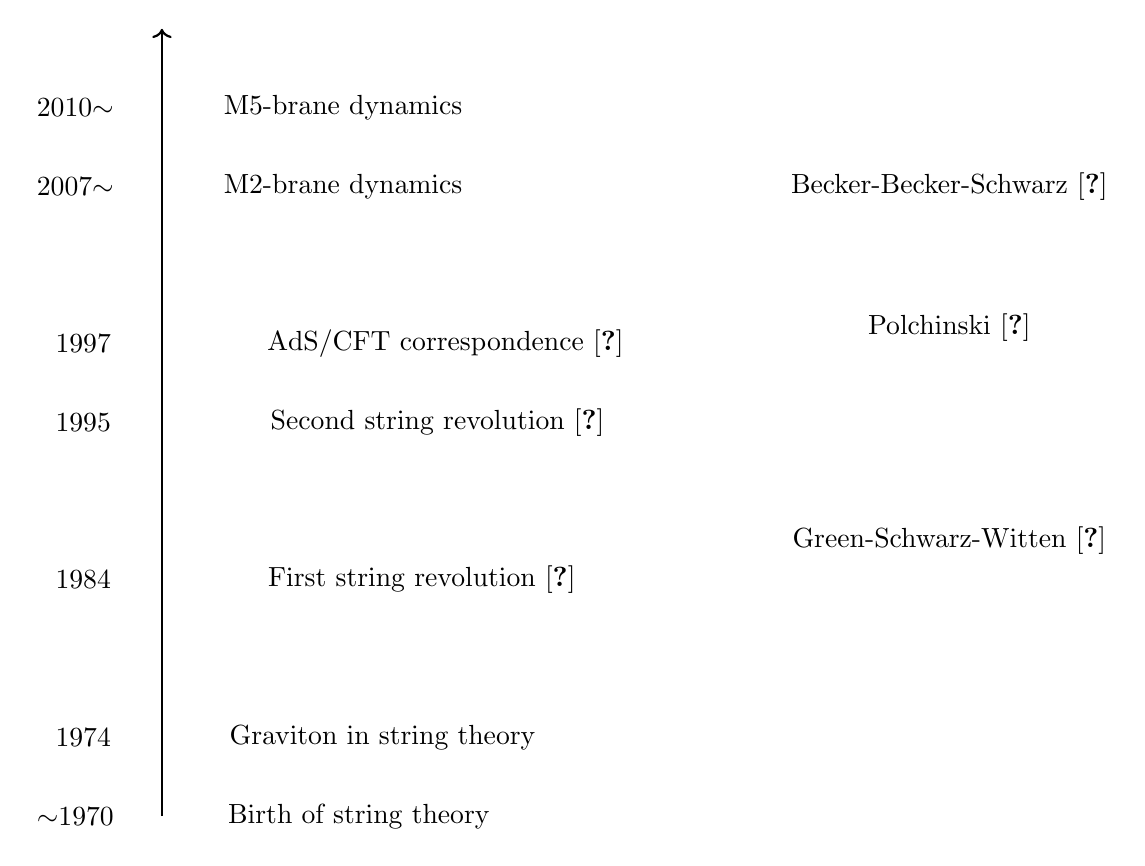
\begin{tikzpicture}
\draw[->,thick]  (0,0) to (0,10);
\node at  (2.3,9) {M5-brane dynamics};
\node at  (-1.1,9) {2010$\sim$}; 
\node at  (10,8) {Becker-Becker-Schwarz \cite{BBS}};
\node at  (2.3,8) {M2-brane dynamics};
\node at  (-1.1,8) {2007$\sim$}; 
\node at  (10,6.2) {Polchinski \cite{Polchinski}};
\node at  (3.6,6) {AdS/CFT correspondence \cite{Maldacena:1997re}};
\node at  (-1,6) {1997};
\node at  (3.5,5) {Second string revolution \cite{Witten:1995ex}};
\node at  (-1,5) {1995};
\node at  (10,3.5) {Green-Schwarz-Witten \cite{GSW}};
\node at  (3.3,3) {First string revolution \cite{Green:1984sg}};
\node at  (-1,3) {1984};
\node at  (2.8,1) {Graviton in string theory};
\node at  (-1,1) {1974};
\node at  (2.5,0) {Birth of string theory};
\node at  (-1.1,0) {$\sim$1970}; 
\end{tikzpicture}
\caption{History of string theory and textbooks}
\end{figure}



\subsection{Very short highlights}


$\bullet$ The basic idea in string theory is different elementary particles are all vibrational modes of a single type of string.  There are two types of strings, open and closed, and a trajectory of a string is called the \textbf{string worldsheet} which is parametrized by $(\sigma,\tau)$. 
If the typical size $\ell_s$  of a string is smaller than the resolution that an accelerator can provide, we cannot see this in the experiment involving elementary particles.
$$
(\textrm{Planck scale})\  10^{-33}\;\textrm{cm}\le \ell_s\le 10^{-17}\;\textrm{cm} \  (\textrm{TeV scale})
$$
We often use the parameter
$$
\a'=\ell_s^2%/(2\pi)^2
$$
which is the only free parameter in string theory. As we will see, the couplings in string theory are expectation values of dynamical fields (so-called moduli) which take their value dynamically.
\begin{figure}[h]\centering
\includegraphics[width=4cm]{openstring}\hspace{2cm}\includegraphics[width=4cm]{closedstring}
\end{figure}

\vspace{.3cm}
\noindent $\bullet$ Application of the rules of quantization provides us with the Fock space of string excitations. In bosonic string, the massless modes include among others 
$$
\begin{array}{c@{\quad }c@{\quad }c@{\quad }c}
\textrm{open string}: & A_\mu & \textrm{spin 1}& \textrm{W-boson}\cr
\textrm{closed string}: & g_{\mu\nu} & \textrm{spin 2}& \textrm{graviton}
\end{array}
$$
In addition, one finds a tower of massive string excitations of mass
\begin{align}
\textrm{open bosonic}: &\quad M^2= \frac{1}{\a'} (N-1) \quad  \cr 
\textrm{closed bosonic}: &\quad  M^2 = \frac{4}{\a'} (N-1)  \quad N = 0,1,2,\ldots \nonumber
\end{align}
Note that the lowest lying state has dimension of negative [mass]${}^2$ $(N=0)$, which is called \textbf{tachyon}. The bosonic theory is consistent only when the number of spacetime dimensions is 26.



\vspace{.3cm}
\noindent $\bullet$ In the point-particle picture, the divergence comes when all four vertices come close to each other. On the other hans, the string word-sheet has no vertices. Thus, when we sum over all surfaces, we do not encounter configuration analogous to collapsed vertices. String theory amplitudes have no ultraviolet (shot distance) divergence.  As a result, string theory provides a finite quantum theory of gravity. Moreover, this is even better than renormalizable quantum field theories since here there is no divergence in the first place. 
\begin{figure}[h]\centering
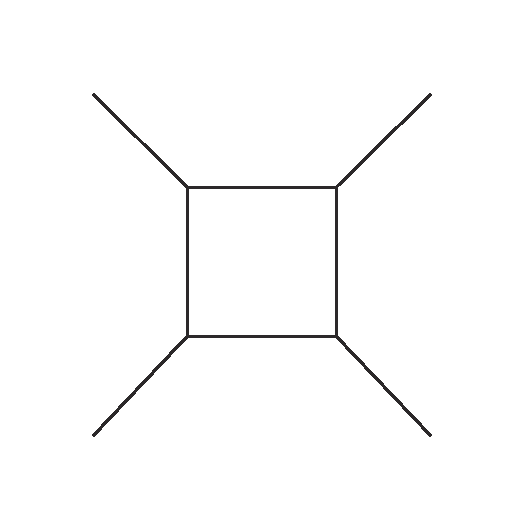
\includegraphics[width=4cm]{Divergence} \hspace{2cm}\includegraphics[width=4cm]{string-loop}
\end{figure}




\vspace{.3cm}
\noindent $\bullet$ 
Strings besides vibrating in usual spacetime can also have some internal degree of freedom. These internal degrees of freedom are fermionic. This can be quantized in a similar manner to that for bosonic strings. Then, a superstring can be considered as a string that has symmetry between bosonic states and fermionic states. In superstring theories, the good feature (e.g. emergence of gravity and UV finiteness) are preserved, and one can incorporate fermions. Moreover, as mentioned,  the tachyonic mode is absent.
\begin{enumerate}
\item the theory is consistent in 10 spacetime dimensions.
\item there are five fully consistent string theories in $d=10$. 

Type IIA, Type IIB, Type I (open+closed string), $E_8\times E_8$ Heterotic, $\SO(32)$ Heterotic

\item Type II theories can have D-branes that accommodate open strings. Type IIA (resp. IIB) has D$p$-branes where $p$ is even (resp. odd), and Type I does D9, D5, D1-branes. 


\item Furthermore all the five apparently different string theories have been found to be different limits of the same underlying theory called  M-theory

\item In the low energy scale $\ll1/ \ell_s$, a theory is described by supergravity which combines supersymmetry and general relativity.

\end{enumerate}




\vspace{.3cm}
\noindent $\bullet$  How do we reduce the number of dimensions from 10 to 4? The answer is Kaluza-Klein mechanism/compactification. 
If we take the 10-dimensional space of the form $\bR^{1,3}\times M$ where $M$ is a 6-dimensional compact space and its size is much smaller than resolution of most powerful  accelerator $\sim 10^{-17}$cm, then a (9+1)-dimensional theory looks like (3+1)-dimensional.  In fact, in order for a theory to be consistent, $M$ has to be a Calabi-Yau manifold (which admits Ricci-flat metric). More importantly, this extra dimensions give ``room'' to derive the complexity of the real world from a simple setting.





\subsection{Convection}
\SN{Summarize convention}
\subsubsection*{Spacetime}
In anticipation of
string theory, we consider $D$-dimensional Minkowski space
${\bR}^{1,D-1}$. Throughout
these notes, we work with signature
%
$$ \eta_{\mu\nu} = {\rm diag}(-1,+1,+1,\ldots,+1)$$
%

\subsubsection*{World-sheet}

It is convenient to introduce complex coordinates and
accordingly vectors, metric etc. 
\begin{itemize}

 \item Coordinates
  \begin{align}\nonumber
   z = x +iy \ , \qquad  \ol z = x -iy \ .
  \end{align}

 \item Derivatives
  \begin{align}\nonumber
   \partial \equiv \partial_z = \frac{\partial}{\partial z} = \frac{1}{2} \left( \partial_1 -i\partial_2 \right) \ ,  \quad
   \ol\partial \equiv \partial_{\ol z} = \frac{\partial}{\partial \ol z} = \frac{1}{2} \left( \partial_1 +i\partial_2 \right) \ ,
  \end{align}
       so that $\partial z = 1$, $\partial \ol z = 0$, $\ol\partial z = 0$, $\ol\partial \ol z = 1$.

 \item Vectors
  \begin{align}\nonumber
   v^z = v^1 +iv^2 \ , \qquad  v^{\ol z} = v^1 -iv^2 \ .
  \end{align}

 \item Metric
  \begin{align}\nonumber
   h_{z\ol z} = h_{\ol z z} = \frac{1}{2} \ , \quad h_{z z} = h_{\ol z\ol z} = 0 \ , \quad
   h^{z\ol z} = h^{\ol z z} = 2 \ , \quad h^{z z} = h^{\ol z\ol z} = 0 \ .
  \end{align}
  So lower-index vectors are $v_z = h_{z\ol z} v^{\ol z} = \frac{1}{2} (v^1-iv^2) $ etc.
 \item Integration measure
  \begin{align}\nonumber
   d^2z = dzd\ol z = 2 dx dy = 2 d^2 x \ ,
  \end{align}
       where the factor $2$ comes from the Jacobian.
       One can also write
  \begin{align}\nonumber
   \sqrt{h} d^2 z = \sqrt{|\det h_{ab}|} d^2 z = d^2x \ .
  \end{align}

 \item Delta function
  \begin{align}\nonumber
   \delta^2(z) = \delta(z)\delta(\ol z) = \frac{1}{2} \delta(x)\delta(y) = \frac{1}{2} \delta^2(x) \ ,
  \end{align}
       so that
  \begin{align}\nonumber
   1= \int d^2z\ \delta^2(z) = \int d^2 x\ \delta^2 (x) \ .
  \end{align}
\end{itemize}
Note that although $z$ and $\ol z$ are complex conjugate of each other,
we will treat them as independent complex numbers.





\section{Bosonic string theory}


\subsubsection*{Nambu-Goto action}


\begin{figure}[h]\centering
\includegraphics[width=4cm]{particle}
\end{figure}


To begin with, let us recall the case of relativistic point particle
$$
\gamma:\tau\to x^\mu(\tau)\in \bR^{1,D-1}~.
$$
The action of relativistic point particle with mass $m$ is 
$$
S=m\int^b_ads=m\int^b_a \Big( -\eta_{\mu\nu}\frac{dx^\mu}{d\tau}\frac{dx^\nu}{d\tau}\Big)^{\frac12}d\tau~.
$$
In a similar fashion, we consider a string
$$ 
\Sigma:(\tau,\sigma)\to X^\mu(\tau,\sigma)\in \bR^{1,D-1}~. 
$$
The analogous action, called the \textbf{Nambu-Goto action}, for the string is given by the area of a string worldsheet $\Sigma$ swept by a string
$$
S_{\textrm{NG}}=T\int_\Sigma \textrm{Area}=T\int_\Sigma d^2\sigma\sqrt{-\det (\g_{ab})}~,\qquad \g_{ab}=\eta_{\mu\nu}\partial_a X^\mu\partial_b X^\nu~
$$
where $(\sigma^0,\sigma^1)=( \tau,\sigma)$, and $T:=1/(2\pi \a')$ is the \textbf{string tension}. The tension is usually defined as mass per unit length.
However, we don't know how to quantize the Nambu-Goto action. Instead, for quantization of string worldsheet, we reformulate the action as follows.


\subsubsection*{String sigma-model action}
Alternatively, we remove the square root and consider the following action
$$
 S_{\sigma}=\frac T2\int d^2\sigma \sqrt{-\det h}~ h^{ab}\partial_a X^\mu \partial_b X^\nu \eta_{\mu\nu}
$$
which is called the \textbf{string sigma-model action}.\footnote{This action is called the Polyakov action in \cite{Polchinski}. However, according to \cite{BBS}, it was discovered by Brink, Di Vecchia and Howe and by Deser and Zumino several years before Polyakov skillfully used it for path-integral quantization of the string. So let's follow the notation of the progenitor, J.H. Schwarz.} Classically the string sigma-model action is equivalent to the Nambu-Goto action. 

\subsubsection*{Symmetry of $ S_{\sigma}$}
\begin{enumerate}
\item\textbf{$D$-dim spacetime Poincare invariance}

The action is certainly invariant under the Poincare transformation
$$ X^\mu(\sigma)\to \L^\mu{}_\nu X^\nu(\sigma)+V^\mu \qquad \Lambda\in \SO(1,D-1)$$ 
where $\L$ is a Lorentz transformation and $V$ is the translation.

\item\textbf{Worldsheet diffeomorphism invariance}

Under the re-parametrization
\begin{align}
\wt X^{\mu}(\wt\sigma)&=X^{\mu}(\sigma)\quad \textrm{with}\quad  \wt{\sigma}= \wt{\sigma}(\sigma)~,\cr
\wt h^{ab}&=h^{cd}\frac{\partial\wt\sigma^a}{\partial\sigma^c}\frac{\partial\wt\sigma^b}{\partial \sigma^d}~,\nonumber
\end{align}
the action is invariant $\wt S(X^\m,h_{ab})=\wt S(\wt X^\m,\wt h_{ab})$. We have two parameter family of gauge symmetry.
\item\textbf{Weyl invariance}

The action is also  invariant under the metric $\wt h_{ab}=e^{\phi(\sigma)}h_{ab}$ by an arbitrary function $\phi(\sigma)$. This symmetry is called the \textbf{Weyl symmetry}.

\end{enumerate}

\subsubsection*{Stress-energy tensor}
The stress-energy tensor is defined by \SN{unify the notation to either stress-energy or energy-momentum tensor}
\begin{align}
T_{ab} &=-\frac{4\pi}{\sqrt{-h}}\,\frac{\partial S}{\partial h^{ab}}\cr
&=-\frac1{\a'} \Big[\partial_a X \partial_b X - \frac12h_{ab}\,\partial_c X \partial^c X\Big]
\end{align}
which satisfies 
\begin{align}
\textrm{traceless}:& \qquad T^a{}_a=0\cr
\textrm{conservation}:& \qquad \nabla_a T^{ab}=0
\end{align}
Note that the traceless condition indeed follows from the Weyl invariance (exercise), and  the conservation can be shown by using the equation of motion for $X^\m$ in the following.
\begin{align}
\frac{\partial S}{\partial h^{ab}}=0&\ \to \ T_{ab}=0\cr
\frac{\partial S}{\partial X^\mu}=0&\ \to \ \Delta X_\mu=-\frac{1}{\sqrt{-h}}\partial_a(\sqrt{-h}h^{ab}\partial_b X^\mu)=0
\end{align}



\subsubsection*{Gauge fixing}
The string sigma-model action $S_\sigma$ is equipped with the symmetries above and we need to fix it for quantization. Physics does not depend on a choice of gauge fixing, but if we choose a clever gauge fixing, our life becomes much easier. Actually, gauge fixing in \cite{BBS} makes our life clearer than that in \cite{Polchinski}, so we use the gauge fixing  in \cite{BBS} as follows.

The metric $h_{ab}$ is a 2$\times$2 symmetric matrix and the woldsheet diffeo invariance tells us that there is a coordinate $\sigma^a$ such that the metric is a diagonal $h_{ab}=e^\omega \eta_{ab}$. Then, the Weyl transformation brings it to the 2d Minkowski metric $\eta_{ab}$. Therefore, one can use $h_{ab}= \eta_{ab}$. If we use the light-cone coordinates on the worldsheet
$$ \sigma^\pm = \tau \pm \sigma\ ,\label{wl}$$
then the metric is written as
$$ds^2=-d\sigma^+d\sigma^-~.$$ 

However, there are residual transformations that leaves the 2d Minkowski metric $\eta_{ab}$ invariant, which is called \textbf{conformal symmetry}:
$$
\sigma^+\to f(\sigma^+) ~, \qquad \sigma^-\to g(\sigma^-) 
$$
with a Weyl transformation simultaneously. To fix the conformal symmetry, we introduce the spacetime light-cone coordinates,
%
$$ X^\pm = \sqrt{\frac{1}{2}}(X^0 \pm X^{D-1}) \ .\label{stlc}$$
%
Then we impose
\be X^+ = x^+ + \a' p^+\,\tau  \ . \label{lcg}~,\ee
which is called \textbf{light-cone gauge}.



\subsubsection*{Mode Expansions}
After the gauge fixing, the the equations of motion simply read
%
$$ \partial_+\partial_- X^\mu = 0\quad \textrm{where} \quad \partial_\pm =\frac12(\partial_\tau\pm\partial_\sigma)~.$$
%
The most general solution is a factorization of left-moving and right-moving waves
%
\be X^\mu(\sigma,\tau) = X^\mu_L(\sigma^+) + X^\mu_R(\sigma^-)\nonumber\ee
%
for arbitrary functions $X^\mu_L$ and $X^\mu_R$. For a closed string, we impose a periodic condition as
\be X^\mu(\sigma,\tau)=X^\mu(\sigma+2\pi,\tau)\ .\label{periodicity}\ee
%
so that the most general can be expanded in Fourier modes
%
\begin{align}\label{mode}
X^\mu_L(\sigma^+) &= \frac12 x^\mu + \frac12 \a' p^\mu \,\sigma^+ + i\sqrt{\frac{\a'}{2}}\sum_{n\neq 0}
\frac{1}{n}\,\wt{\alpha}_n^\mu\, e^{-in\sigma^+} \ ,\cr
X^\mu_R(\sigma^-) &= \frac12 x^\mu + \frac12 \a' p^\mu \,\sigma^- + i\sqrt{\frac{\a'}{2}}\sum_{n\neq 0}
\frac{1}{n}\,{\alpha}_n^\mu\, e^{-in\sigma^-} \ ,
\end{align}
%
where the reality of $X^\mu$ requires that the coefficients of the Fourier modes obey
%
$${\alpha}_n^\mu= (\alpha^\mu_{-n})^\ast\ \ \ ,\ \ \ \wt{\alpha}_n^\mu=(\wt{\alpha}^\mu_{-n})^\ast\ .\label{realalpha}$$
%
This mode expansion will be very important when we come to the quantum theory. We have to keep in mind that we have to impose  the equation of motion
\be\label{constraints}
T_{--}=(\partial_-X)^2 =0\qquad T_{++}= (\partial_+ X)^2 = 0~.
\ee
We will see the implication of these constraints in the quantum theory.






\subsubsection*{Quantizations}
The momentum conjugate to $X^\mu$ is defined in this gauge
$$
\Pi_\mu=\frac{\delta S}{\delta (\partial_\tau X^\mu)}=T\; \partial_\tau X^\mu~.
$$
The canonical quantization promotes $X^\mu$ and $\Pi_\mu$ to operators that is subject to
%
\begin{align} 
&[X^\mu(\sigma,\tau),\Pi_\nu(\sigma^\prime,\tau)]=i\delta(\sigma-\sigma^\prime)
\,\delta^\mu_{\ \nu} &\ , \cr 
&[X^\mu(\sigma,\tau),X^\nu(\sigma^\prime,\tau)] = [\Pi_\mu
(\sigma,\tau),\Pi_\nu(\sigma^\prime,\tau)] = 0&\ .\nonumber\end{align}
%
We translate these into commutation relations for the Fourier modes $x^\mu$, $p^\mu$, ${\alpha}_n^\mu$ and $\wt {\alpha}_n^\mu$. Using the mode expansion, we find (exercise)
%
\be [x^\mu,p_\nu]=i\delta^\mu_{\ \nu} \ \ \ {\rm and}\ \ \
{[}{\alpha}_n^\mu,\alpha_m^\nu{]}=
{[}\wt {\alpha}_n^\mu,\tilde{\alpha}_m^\nu{]}
=n\, \eta^{\mu\nu}\delta_{n+m,\,0}\ ,\label{acom}\ee
Therefore, like harmonic oscillators, the creation operators are $\a_{-n}^{\m},\wt \a_{-n}^{\m}$ and the annihilation operators are $\a_{n}^{\m},\wt \a_{n}^{\m}$ for $n\in\bN$ so that the Hilbert space is spanned by
$$
\a_{-n_1}^{\m_1}\cdots \a_{-n_k}^{\m_k} \wt\a_{-n_1}^{\m_1}\cdots \wt\a_{-n_k}^{\m_k}|k\rangle   \qquad \textrm{where} \qquad p^\m|k\rangle=k^\m|k\rangle~.
$$

Let us consider the implication of the constraints \eqref{constraints}. Using the mode expansions \eqref{mode}, the stress-energy tensor can be expressed as
$$
T_{--}=\a'\sum_n L_ne^{-in\sigma^-} \qquad T_{++}=\a'\sum_n \wt L_ne^{-in\sigma^+}
$$
where 
\begin{align}\label{Virasoro}
L_m=\frac12 \sum_{n\neq0} \eta_{\m\n} :\a^\m_{m-n}\a^\n_n: \qquad 
\wt L_m=\frac12 \sum_{n\neq0} \eta_{\m\n} :\wt \a^\m_{m-n}\wt \a^\n_n:  
\end{align}
with $\a_0^\m=\wt \a_0^\m=\sqrt{\frac{\a'}{2}}p^\m$. We will learn $L_m$ are generators of \textbf{Virasoro algebra}.  According to the normal-ordering $: \ :$ prescription, the lowering operators always appear to the right of the raising operators. However, it is easy to see that the normal ordering matters only in $L_0$ and $\wt L_0$.
Thus, in the quantum theory, the constraint \eqref{constraints} on the stress-energy tensor can be interpreted by
$$L_n| \textrm{phys} \rangle =0 \qquad \wt L_n| \textrm{phys} \rangle =0 \qquad \textrm{for} \quad n>0$$
so that
$$
\langle \textrm{phys}'| L_n | \textrm{phys} \rangle =0 \qquad  \langle \textrm{phys}'| \wt L_n | \textrm{phys} \rangle =0 \qquad \textrm{for} \quad n>0~.
$$




\subsubsection*{Light-cone quantization}
To see the effect of normal ordering in $L_0$, let us consider the meaning of the light-cone gauge \eqref{lcg} in the quantum theory. It is easy to see that \eqref{lcg} implies
$$
\a_n^+=0 \quad \textrm{for} \quad n\neq0~.
$$
Then, the equation of motion
$$
 2\partial_+X^-\partial_+X^+=\sum_{i=1}^{D-2}\partial_+X^i\partial_+ X^i 
$$
tells us
$$
 \alpha^-_n = \sqrt{\frac{1}{2\a'}}\frac{1}{p^+}\sum_{m=-\infty}^{+\infty}\sum_{i=1}^{D-2} \alpha_{n-m}^i\alpha^i_m~.
$$
In particular, for $n=0$, we have
$$
M^2 = 2p^+p^- - \sum_{i=1}^{D-2}p^ip^i = \frac{4}{\a'}\left(\sum_{n>0}\sum_{i=1}^{D-2}  \alpha_{-n}^i\alpha_n^i + \frac{D-2}{2}\sum_{n>0} n\right)
$$
The final term clearly diverges. Fortunately, we have nice regularization of this divergence
\begin{align} \sum_{n=1}^\infty n\  \longrightarrow \ \sum_{n=1}^\infty n e^{-\epsilon n} &= -\frac{\partial}{\partial \epsilon}\sum_{n=1}^\infty e^{-\epsilon n} \nonumber\\ &= -\frac{\partial}{\partial\epsilon} (1-e^{-\epsilon})^{-1} \nonumber\\
% &=& \frac{e^\epsilon}{(e^\epsilon -1)^2} \nonumber\\
&= \frac{1}{\epsilon^2}-\frac{1}{12}+{\cal O}(\epsilon)\nonumber\end{align}
%
Obviously the $1/\epsilon$ piece diverges as $\epsilon\rightarrow 0$. This term should be renormalized
away so that we have
%
$$ \sum_{n=1}^\infty n = -\frac{1}{12} \ .$$
%
Hence, we obtain
\be \label{mass} M^2 = \frac{4}{\a'}\left(N-  \frac{D-2}{24} \right)
= \frac{4}{\a'}\left(\wt{N} - \frac{D-2}{24} \right)
\ ,\ee
where 
the number operators are defined by
%
$$ N = \sum_{i=1}^{D-2}\sum_{n>0} \alpha^i_{-n}\alpha_n^i\ \ \  ,\ \ \ \tilde{N} = \sum_{i=1}^{D-2}\sum_{n>0} \tilde{\alpha}^i_{-n}\tilde{\alpha}_n^i \ .\label{nntilde}$$
%
It is easy to see  from \eqref{mass} 
\be\label{lmc}
N=\wt N
\ee
which is called the \textbf{level-matching condition}. Moreover, if $D>2$, we have the state with negative [mass]${}^2$ for $N=0=\wt N$ which is called the \textbf{tachyon}.




\subsubsection*{The First Excited States}

We now look at the first excited states. If we act with a creation operator $\alpha^j_{-1}$, then
the level matching condition \eqref{lmc} tells us that we also need to act with a
$\tilde{\alpha}_{-1}^i$ operator. This gives us $(D-2)^2$ particle states,
%
\be \tilde{\alpha}_{-1}^i\alpha_{-1}^j\,|0;p\rangle \ ,\label{first}\ee
%
each of which has mass
%
\be M^2 = \frac{4}{\a'}\left(1-\frac{D-2}{24}\right)\ .\nonumber\ee
%
It is easy to see that the state is under a representation of the little group $\SO(D-2)\subset \SO(1,D-1)$ and therefore it should be massless. Interestingly, this is only the case if the dimension of spacetime is
%
\be D=26\ .\nonumber\ee
%
This is our first derivation of the critical dimension of the bosonic string.


Moreover, the states \eqref{first} transform in the ${\bf 24}\otimes {\bf 24}$ representation of $\SO(24)$.  These decompose into three irreducible representations:
%
\be \mbox{traceless symmetric} \ \oplus\ \mbox{anti-symmetric}\ \oplus\ \mbox{singlet (=trace)}\nonumber\ee
%
To each of these modes, we associate a massless field in spacetime such that the string oscillation can be identified with a quantum of these fields. The fields are:
%
\be G_{\mu\nu}(X)\ \  \ ,\ \ \ \ \ B_{\mu\nu}(X)\ \ \ \ \ ,\ \ \ \ \ \Phi(X)\ee
%



















\SN{Need to edit}


Note that in this lecture we use $\alpha'$ rather than string tension $T = \frac{1}{2\pi\alpha'}$.
World-sheet(WS) index here is denoted by $a, b$ rather than $\alpha, \beta$.
$h_{ab}$ is WS metric; do not confuse with the induced metric $h_{\alpha\beta} = \eta_{\mu\nu} \partial_\alpha X^\mu \partial_\beta X^\nu$
used in the last lecture.
Convention in this note basically follows Polchinski's one, though
we adopt slightly different normalization for Noether current in \S\ref{sec:Noether}.


\subsection{Towards string interaction}

What we have learnt is
\begin{itemize}
% \item Nambu-Goto action $\sim$ String sigma model (by introducing),
% \item Weyl invariance (inv) $\times$ world-sheet (WS) diffeomorphism (diff) is important,
 \item Mass spectrum of a string by light-cone quantization in flat space-time (ST).
\end{itemize}
What we have NOT learnt is
\begin{itemize}
 \item string interactions,
 \item extension to curved background (curved ST).
\end{itemize}
Especially because of the first reason(string interaction)
we want to express our analysis in terms of \textit{path integral},
which is more natural to illustrate string interaction.
(If you are not familiar with path integral, consult the appendix of Polchinski Vol.1. for derivation.)
See Fig.~\ref{fig1}, which is a naive but appropriate extension from quantum field theory (QFT) interaction to string interaction.
\begin{figure}[htb]
 \centerline{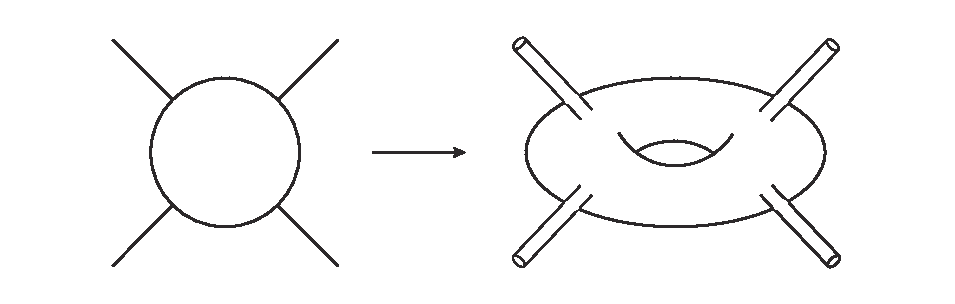
\includegraphics[width=250pt]{fig1}}
 \caption{A Feynman diagram of QFT (left) and a string interaction diagram (right). Each end of the cylinders connecting to the torus(Riemann surface) in the string interaction diagram corresponds to an initial/final state.}
 \label{fig1}
\end{figure}
Each end of the cylinders in the Figure corresponds to an initial/final state of string.
It is quite cumbersome to use \textit{state} expression.
Instead, we will use vertex operator $\wh V$ to express those states, which is explained in the following subsection.
Given that we adopt the operator expression the string interaction is written as in Fig.~\ref{fig2} as well as
\begin{align}\nonumber
 A_n = \sum_g \int \left(\cD h_{ab}\right)_{g,n} \int \cD X^\mu e^{-S_\sigma [X^\mu,h_{ab}]} \wh V_1 \cdots \wh V_n \ ,
\end{align}
where $n$ is the number of in-coming/out-going strings, and $g$ is the number of holes(genus) of the Riemann surface (genus is $1$ in the figures).
\begin{figure}[htb]
 \centerline{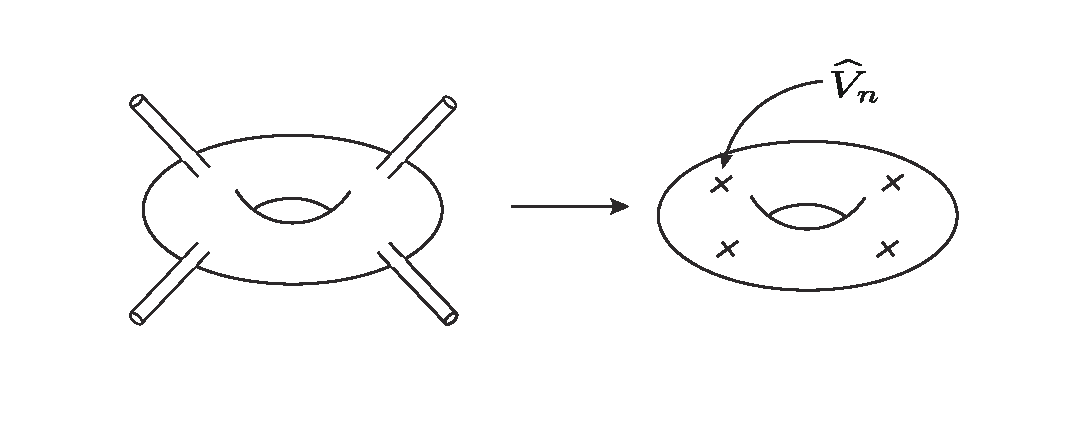
\includegraphics[width=250pt]{fig2}}
 \caption{String interaction in state expression (left) and operator expression (right).}
 \label{fig2}
\end{figure}

\subsection{Path integral method}

% As a short goal of studying string theory, we want to know the spectra of a closed/open string,
% and how to describe string interactions.

% The operator analysis is a tool to achieve these purposes.
% This is because the string world sheet theory is a conformal field theory


In path integral method expectation values(partition function, 2pt func etc.) are given in the following form
\begin{align}\nonumber
 \langle \mathcal O[X] \rangle = \int \cD X e^{iS[X]} \mathcal O [X] \ ,  \qquad
 S = \frac{1}{4\pi \alpha'} \int d\sigma d\tau \left\{ \left(\partial_\tau X\right)^2 -\left(\partial_\sigma X\right)^2\right\} \ ,
\end{align}
where $\mathcal O$ is an arbitrary operator (eg. for partition function $\mathcal O = 1$, for 2pt func $\mathcal O = X^\mu X^\nu$).
Note that we often omit the (super-)sub-script $\mu$ if it is not crucial.
% $S[X]$ etc. are called functional.
We usually \textbf{Wick rotate} ($\tau \to -it$) the theory so that it converges.
\begin{align}\nonumber
 \langle \mathcal O[X] \rangle = \int \cD X e^{-S_E[X]} \mathcal O [X] \ ,  \qquad
 S_E = \frac{1}{4\pi \alpha'} \int d\sigma dt \left\{ \left(\partial_t X\right)^2 +\left(\partial_\sigma X\right)^2\right\} \ .
\end{align}
The subscript $E$ will be omitted hereafter, and we will always work in the WS Euclidean signature.


(Even if you do not know path integral well) What we need to understand (at least for today) is that we can manipulate it as like normal integral:
\begin{itemize}
 \item total derivative vanishes (assumption)
  \begin{align}\nonumber
   0 = \int \cD X \frac{\delta}{\delta X} \left( e^{-S_E[X]} \mathcal O [X] \right) \ .
  \end{align}
% \item it commutes with derivatives
\end{itemize}
Note that with subscripts the functional derivative gives
\begin{align}\nonumber
 \frac{\delta X^\mu (w)}{\delta X^\nu (z)} = \delta^\mu_\nu \delta^2(z-w) \ .
\end{align}

\subsection{State-operator correspondence}


As we have seen the string sigma model is Weyl invariant:
\begin{align}\nonumber
 S_\sigma \left[ X^\mu, h_{ab} \right] = S_\sigma \left[ X^\mu, e^{\phi(\sigma)} h_{ab} \right] \ .
\end{align}
This (and together with WS diff) can be regarded as a property of the matter theory as we saw in the previous lecture,
and we say that matter theory of $X$ is conformally invariant or the matter theory is a conformal field theory (CFT).
We can use this freedom to set WS to be $\bR^2$ (recall that the topology of (closed) string is cylinder).
\begin{align}\nonumber
 \bR^2:  \quad ds^2 &= dx^2 +dy^2 = dr^2 +r^2 d\theta^2 \cr
 &= r^2 \left[ d\left(\log r\right)^2 +d\theta^2 \right] \ ,
 \textrm{Cylinder} : \quad ds^2 &= dt^2 +d\sigma^2 \ ,
\end{align}
where the overall factor $r^2$ in $\bR^2$ is identified with the Weyl factor $e^{\phi(\sigma)}$, and can be removed.
So we can identify:
\begin{align}\nonumber
 t = \log r \ ,  \qquad  \sigma = -\theta \ .
\end{align}
The reason for the minus sign will be clear later.
This identification tells us that there is a correspondence between
\begin{itemize}
 \item CFT on a semi-infinite cylinder $(\sigma, t;\ t \le 0)$ , and
 \item CFT on a disk $(x^2+y^2 \le 1)$ with the origin removed  ,
\end{itemize}
provided that we choose the boundary conditions to be the same.
Especially, the initial \textit{state} of the string ($t = -\infty$) corresponds to a \textit{local operator}
inserted at the origin, which is called vertex operator (see Fig.~\ref{fig3}).
\begin{figure}[htb]
 \centerline{\includegraphics[width=250pt]{fig3}}
 \caption{State-operator correspondence. Initial state(red circle) is mapped to a local operator(red dot) at the origin.}
 \label{fig3}
\end{figure}
This is the state-operator correspondence and we will express string states by the vertex operators
(see again Fig.~\ref{fig2}).


Now you may wonder if there is any way to express commutation relations in terms of operators
so that we can do parallel procedures of the canonical quantization in terms of operators.
This is what we do in the next section.







\section{Two-dimensional conformal field theories}


Conformal field theories (CFTs) play distinctive role in quantum field theories, string theory, statistical mechanics, and condensed matter physics. Moreover, 2d CFTs are particularly rich because of infinite dimensional symmetry \cite{belavin1984infinite}. In the previous lecture, we have studied an important property of conformal field theories, the state-operator correspondence. In this lecture, we will learn significant feature of 2d conformal field theories more in detail. However, we glimpse only a tip of iceberg  and the subject would actually deserve the entire one semester. If you are interested in this fertile subject, we refer to the standard references \cite{ginsparg1988applied,francesco2012conformal,Blumenhagen:2009zz}.


\subsection{Conformal transformations}

 A CFT in any dimension is a quantum field theory which is invariant under conformal transformations at quantum level.
A \textbf{conformal transformation} is a change of coordinates
$x^a\rightarrow \wt{x}^a(x)$ such that the metric changes by
%
\be g_{ab}(x) \rightarrow \Omega^2(\sigma)g_{ab}(x)~.\label{cft}\ee
%
This means that the theory behaves the same at
all length scales. 

In the string sigma model action,  the metric is dynamical and the conformal transformations \eqref{cft} consist of a subgroup of diffeomorphisms so that it can be canceled by a Weyl symmetry of the metric. However, in the following, we fix a 2d Euclidian flat metric and  the transformation \eqref{cft} should be thought of as physical symmetry, taking the point $x^\alpha$ to point $\wt{x}^\alpha$.



\begin{figure}[h]\centering
\includegraphics[width=13cm]{conformal-trans}
\end{figure}
\subsubsection*{2d flat space}
In complex coordinate, the 2d flat metric can be written as $ds^2 = dz d\bar{z}$. Under a holomorphic map,
$$
z\rightarrow f(z)~,
$$
the metric is transformed as
$$
ds^2 = dz d\bar{z}\quad  \rightarrow\quad  ds^2 =\frac{\partial {f}}{\partial {z}} \frac{\partial \bar{f}}{\partial \bar{z}} dz d\bar{z}~. 
$$
Therefore, all the holomorphic maps are conformal transformations where  $\left| \frac{\partial f}{\partial z} \right|^2$ is a conformal factor (corresponding to $ \Omega^2(\sigma)$ in \eqref{cft}). Moreover, it is easy to show that all 2d conformal transformations are indeed holomorphic functions (Exercise).  This set is infinite-dimensional, corresponding to the the coefficients of the Laurent series of holomorphic functions in some neighborhood. This infinity is what makes conformal symmetry so powerful in two dimensions.

%To consider an infinitesimal conformal transformation, we right $f(z)=z+\epsilon(z)$. Because $f(z)$ is a holomorphic function, so too is $f(z)=z+\epsilon(z)$. The same statements hold true for the variable $\bar{z}$. These facts mean that metric tensor transforms as
%$$
%ds^2 = dz d\bar{z} \rightarrow \frac{\partial {f}}{\partial {z}} \frac{\partial \bar{f}}{\partial \bar{z}} dz d\bar{z}. 
%$$
%We can also read off the scale factor for these 2d conformal transformations as $\Lambda = \left| \frac{\partial f}{\partial z} \right|^2$.
%

\SN{Need to edit}


We will learn operator analysis of 2d conformal field theory (CFT), including OPE, Ward-Takahashi identity etc.,
and we will see Virasoro algebra, which is associated to the conformal symmetry.


% As we have learnt in the last lecture the conformal transformations are arbitrary holomorphic/anti-holomorphic local translation.
% The action is invariant under the transformation






\subsection{Massless scalar theory in 2d}


We study massless scalar fields as the easiest example.
We adopt Euclidean metric $\eta_{ab} = \textrm{diag}(+,+)$, though the procedure is parallel for Lorentz metric.
The action of massless scalar fields $X^\mu$ ($\mu = 1, 2,\ldots,D$) is given by
\begin{align}\nonumber
 S_\mathrm{} = \frac{1}{4\pi\alpha'} \int d^2x \ \left( \partial_1 X \cdot \partial_1 X +\partial_2 X \cdot \partial_2 X \right) \ ,
\end{align}
where $d^2x = dx_1dx_2$, $x_1 = x$, $x_2 =y$, and $\partial_i = \frac{\partial}{\partial x_i}$.
(The subscript E will be omitted hereafter.)



% Note that we are following Polchinski's notations rather than Hosomichi's.

\textbf{Stokes' theorem} (it is called Green's theorem in 2d) will be used frequently.
\begin{align}\nonumber
 \int_D d^2z \left( \partial \ol V + \ol\partial V\right)
 = \frac{1}{i} \oint_{\partial D} \left( V dz - \ol V d\ol z \right) \ ,
\end{align}
where $D$ is an arbitrary region (typically small disk) and $\partial D$ is its boundary.
$V$ and $\ol V$ are independent factor.
Using the Stokes' theorem one can prove following equation.
\begin{align}
 \partial\ol\partial \log |z|^2 =2\pi \delta^2(z) \ .
 \label{eq:deltaFunc}
\end{align}
(Keep this in mind. We will use this later.)



With the complex coordinate convention, the action becomes
\begin{align}\nonumber
 S = \frac{1}{2\pi\alpha'} \int d^2 z\ \partial X \cdot \ol\partial X
 \quad
 \left( = \frac{1}{4\pi \alpha'}\int \sqrt h d^2z\ h^{ab} \partial_a X \cdot \partial_b X \right) \ .
\end{align}
The equation of motion (E.O.M) is given by
\begin{align}\nonumber
 \delta S &= \frac{1}{2\pi \alpha'} \int d^2z \left( \partial X \cdot \ol\partial (\delta X) +\partial (\delta X) \cdot \ol\partial X \right)  \cr
 &= -\frac{1}{\pi \alpha'} \int d^2z\ \delta X \cdot \partial\ol\partial X  =0 \ ,  \cr
 \therefore & \quad \partial\ol\partial X^\mu = 0 \ .
\end{align}
General solution to the E.O.M is
\begin{align}\nonumber
 X^\mu(z,\ol z) &= X_R^\mu (z) +X_L^\mu (\ol z)   ,   \cr
 X_R^\mu (z) &= \frac{1}{2}x^\mu -i \frac{\alpha'}{2} p^\mu \log z +i \sqrt{ \frac{\alpha'}{2} } \sum_{n \neq 0} \frac{1}{n} \frac{\alpha_n^\mu}{z^n} \ , \cr
 X_L^\mu (\ol z) &= \left. X_R^\mu (\ol z) \right|_{\alpha_n \to \wt \alpha_n} \ .
\end{align}
Notice that
\begin{align}\nonumber
 z &= r e^{i\theta} = e^{\log r +i\theta} = e^{i\tau -i\theta}  \cr
   &= e^{i\sigma^-} \ ,  \cr
 \ol z &= e^{i\sigma^+} \ ,
\end{align}
and compare to
\begin{align}\nonumber
 X^\mu_R(\sigma^-) &= \frac{1}{2} x^\mu + \frac{1}{2} \alpha' p^\mu \,\sigma^- + i\sqrt{\frac{\alpha'}{2}}\sum_{n\neq 0}
\frac{1}{n}\,{\alpha}_n^\mu\, e^{-in\sigma^-} \ .
\end{align}




\subsection{Operator analysis (Path integral quantization)}



Let us consider quantum version of the E.O.M by using a path integral formulation.
% Correlation function of an operator $\mathcal O$ is given by a path integral
% \begin{align}\nonumber
%  \langle \mathcal O \rangle = \int \mathcal D \Phi e^{-S[\Phi]} \mathcal O[\Phi]  .
% \end{align}
As like a normal integral we assume that ``total derivative'' vanishes in path integral.
For example, in the massless free scalar case we have
\begin{align}\nonumber
 0 = \int \mathcal D X \ \frac{\delta}{\delta X} e^{-S[X]} = \int \mathcal D X \ e^{-S[X]} \frac{1}{\pi\alpha'}\partial\ol\partial X
 = \frac{1}{\pi\alpha'} \langle \partial\ol\partial X \rangle \ ,
\end{align}
which is nothing but Ehrenfest's theorem.
The E.O.M is satisfied as an operator equation if there is no other operator nearby.


Furthermore, the same procedure can be done with operator insertions.
The easiest example is
\begin{align}\nonumber
 0 = \int \mathcal D X \ \frac{\delta}{\delta X_\mu (z,\ol z)} \left(e^{-S[X]} X^\nu (w,\ol w) \right)
 = \langle \frac{1}{\pi\alpha'}\partial_z\partial_{\ol z} X^\mu (z,\bar z) X^\nu(w,\bar w) + \eta^{\mu\nu}\delta^2(z-w) \rangle \ .
\end{align}
Therefore,
\begin{align}\nonumber
 \partial\ol\partial X^\mu (z,\bar z) X^\nu(w,\bar w) = -\pi\alpha' \eta^{\mu\nu}\delta^2(z-w) \ ,
\end{align}
where note that this is operator equation (not classical equation) and we simply omitted $\langle \rangle$ symbols.
The right hand side is understood due to a quantum effect.

Recalling Eq.~(\ref{eq:deltaFunc}) we have
\begin{align}\nonumber
 X(z,\bar z)^\mu X^\nu(w,\bar w) = -\frac{\alpha'}{2} \eta^{\mu\nu} \log |z-w|^2 + \nord{X(z,\bar z)X(w,\bar w)} \ ,
\end{align}
where we introduced normal ordering $\nord{\mathcal O}$, meaning that the divergence at $z \to w$ has been subtracted.
We also write it as follows.
\begin{align}\nonumber
 \nord{X^\mu(z,\bar z)X^\nu(w,\bar w)} = X^\mu(z,\bar z)X^\nu(w,\bar w) -\eta^{\mu\nu}G(z,w) \ ,
\end{align}
where $G(z,w) = -\frac{\alpha'}{2} \log|z-w|^2$.
Notice that
\begin{align}
 \partial_z \partial_{\ol z} \nord{X(z,\bar z)X(w,\bar w)} = 0 \ .
 \label{eq:normalEOM}
\end{align}
As we will see later the divergent term is important and meaningful.
This is why it is convenient to introduce the normal ordering so that we can separate the divergent terms from the other.



For an arbitrary functional of fields the OPE is expressed as follows.
% \begin{align}\nonumber
%  \nord{X_1 X_2 \cdots X_n} = X_1 X_2 \cdots X_n -\sum_\textrm{1 pair} G_{i_1 i_2} X_{i_3} \cdots X_{i_n}
%  +\sum_\textrm{2 pairs} G_{i_1 i_2} G_{i_3 i_4} X_{i_5} \cdots X_{i_n} -+ \cdots  .
% \end{align}
\begin{align}\nonumber
 \nord{f[X]} = \exp \left[ -\frac{1}{2} \int d^2z d^2w\ G(z,w) \frac{\delta}{\delta X^\mu(z,\bar z)} \frac{\delta}{\delta X_\mu(w,\bar w)} \right]
 f[X] \ .
\end{align}
For example,
\begin{align}\nonumber
 \nord{X_1X_2X_3X_4X_5} =& X_1X_2X_3X_4X_5 -\left( G_{12}X_3X_4X_5 +\cdots \right)_\textrm{10 terms}  \cr
 &+\left( G_{12}G_{34}X_5 +\cdots \right)_\textrm{15 terms} \ ,
\end{align}
where $X_i=X(z_i)$ and $G_{ij} = G(z_i,z_j)$.


Multiplication of normal ordered product is given as follows.
\begin{align}\nonumber
 \nord{f[X]} \nord{g[X]} = \exp \left[ \int d^2z d^2w\ G(z,w) \left. \frac{\delta}{\delta X^\mu(z,\bar z)} \right|_{f} \left. \frac{\delta}{\delta X_\mu(w,\bar w)} \right|_{g} \right] \nord{fg[X]} \ .
\end{align}
Example 1:
\begin{align}\nonumber
 \nord{ \partial X(z,\bar z)} \nord{ X(w,\bar w)} = \nord{\partial X(z,\bar z) X (w,\bar w)} +\partial_z G(z,w)  
 = \nord{\partial X (z,\bar z) X (w,\bar w)} -\frac{\alpha'}{2} \frac{1}{z-w} \ .
\end{align}
Example 2:
\begin{align}\nonumber
 \nord{e^{ik\cdot X(z,\bar z)}} \nord{e^{ik'\cdot X(w,\bar w)}} &= \exp\left[ (ik) \cdot (ik') \left( -\frac{\alpha'}{2} \log|z-w|^2 \right)\right]
 \nord{e^{ik\cdot X(z,\bar z) +ik'\cdot X(w,\bar w)}} \cr &= |z-w|^{\alpha'k\cdot k'} \nord{e^{ik\cdot X(z,\bar z) +ik'\cdot X(w,\bar w)}} \ .
\end{align}






\subsection{Operator product expansion (OPE)}


In general field theory, product of a pair of fields can be expanded by a single operator
\begin{align}\nonumber
 \Phi^i (z) \Phi^j (w) = \sum_{k} C^{ij}_k(z-w) \Phi^k (w) \ .
\end{align}
% We omit the second variable $\ol z$ hereafter (namely, $\Phi(z)=\Phi(z,\ol z)$).
Note that in 2d CFT language any local operator is regarded as an independent field (e.g. $\Phi = X, \partial X, \nord{XX}$ etc.).


Typically, for a massless free scalar field theory we have
\begin{align}\nonumber
 &X^\mu (z,\ol z) X^\nu (w,\ol w) =  -\frac{\alpha'}{2} \eta^{\mu\nu} \log |z-w|^2 +\nord{X^\mu X^\nu (w,\ol w)}  \cr
 &\qquad +\sum_{k=1}^\infty \frac{1}{k!} \left\{ (z-w)^k  \nord{\partial^k X^\mu X^\nu (w, \ol w)}
 +(\ol z-\ol w)^k  \nord{\ol\partial^k X^\mu X^\nu (w, \ol w)}\right\} \ .
\end{align}
The second and the third terms of RHS can be understood as Taylor expansion of $\nord{X(z)X(w)}$ in terms of $z$. Mixing terms ($\nord{\partial^m\ol\partial^n X X}$) vanish due to ``E.O.M'', Eq.~(\ref{eq:normalEOM}).


As we will see, only the divergent term is important.
We will introduce $\sim$ that is define as ``equal up to non-divergent term''
so that we can forget about non-divergent terms.
For example
\begin{align}\nonumber
 X^\mu (z,\ol z) X^\nu (w,\ol w) \sim  -\frac{\alpha'}{2} \eta^{\mu\nu} \log |z-w|^2 \ .
\end{align}



\subsection{Noether's theorem and Ward-Takahashi identities}\label{sec:Noether}

When an action is invariant under a certain transformation $\delta$ (namely, $\delta S = 0$)
we say the theory has a (classical) symmetry.
Furthermore, the measure of the path integral is also invariant under the
transformation we say the theory has a symmetry at quantum level.
On the other hand, if the measure is not invariant, then, we say the theory has anomaly and/or the symmetry is anomalous.
It is non-trivial to see if the theory has anomaly or not.

If the theory has a symmetry there is a corresponding conserved current $j^a$
and the space integral of its time component is the conserved charge $Q=\int_\textrm{space} j^0$, which generate the symmetry $\delta X = [Q, X]$.
The current can be derived by Noether's procedure.
Even if you are not familiar with the Noether's theorem
we will see alternative method.


Let $\delta$ be a symmetry $\delta S = 0$ and assume it acts on a field as follows: $\delta X (z) = \epsilon (\cdots) $, where $\epsilon$ is a small parameter.
If we promote the parameter to be WS coordinate dependent (i.e. $\wh \delta X = \epsilon(z,\ol z) (\cdots)$), then $\wh \delta S$ is no longer zero but has to take the following form.
\begin{align}\nonumber
 \wh\delta S = \int \frac{d^2 x}{2\pi} \epsilon(x,y) \partial_a j^a
 = \int \frac{d^2z}{2\pi} \epsilon(z, \ol z)
 \left( \partial \ol j +\ol\partial j \right) \ ,
\end{align}
where we introduced $j = j_{z}$ and $\ol j = j_{\ol z}$.
If the parameter is constant $\delta S = (\textrm{total derivative}) = 0$.
\textbf{ $j^a$ is Noether current}.
Noether current is conserved, which means that $\partial_a j^a = 0$ under assumption of E.O.M.
This implies that $j$($\ol j$) is a holomorphic(anti-holomorphic) function of $z$.
Indeed, this is true for all the example we will see.


\subsubsection*{Ward-Takahashi identity}

Now let us study the transformation of  a point operator $\mathcal{O}[X](w,\ol w)$ under the symmetry $\delta$. For this purpose, 
we set
\begin{align}\nonumber
 \epsilon(z,\ol z) =
 \begin{cases}
  \epsilon \quad (\textrm{const.}) \quad &\textrm{for}\ z \in D_w \ ,  \cr
  0                                      &\textrm{for}\ z \not\in D_w \ , \cr
 \end{cases}
\end{align}
where $D_w$ is a disk containing $w$. Then, the variation of the path integral
\begin{align}\nonumber
 0 = \int \cD X \ \wh \delta \left[ e^{-S} \mathcal{O}(w,\ol w) \right]
 = \int \cD X e^{-S}\  \left[ \delta \mathcal{O}(w,\ol w) -\wh \delta S \cdot \mathcal{O}(w,\ol w) \right]  .
\end{align}
Therefore, we have
\begin{align}\nonumber
 \delta \mathcal{O}(w,\ol w) &= \int \frac{d^2z}{2\pi} \epsilon(z, \ol z)
 \left( \partial \ol j(\ol z) +\ol\partial j(z) \right) \mathcal{O}(w, \ol w)  \cr
 &= \frac{\epsilon}{2\pi i} \oint_{\partial D_w} \Big( dz\ j(z) -d\ol z\ \ol j(\ol z) \Big) \mathcal{O}(w,\ol w) \ ,
\end{align}
This is called the \textbf{Ward-Takahashi identity}.


Let us see an example of the free scalar field.
\begin{align}\nonumber
 &S = \frac{1}{2\pi \alpha'} \int d^2z\ \partial X \cdot \ol\partial X \ ,  \qquad
 \delta X = \epsilon g(z)  \quad (\textrm{holomorphic})  \cr
 \to \quad &\wh \delta S = \frac{-2}{2\pi \alpha'} \int d^2z\ \epsilon(z,\ol z) \ol\partial \left( g \partial X\right)  \cr
 &j = -\frac{2}{\alpha'} g \partial X \ , \qquad  \ol j = 0  .
\end{align}
Check that $\delta X(w) = \epsilon \oint_{\partial D} \frac{dz}{2\pi i}\ j(z) X(w) $ is consistent.




\subsection{Conformal Ward-Takahashi identity}




Recall that  in a field theory, continuous symmetries correspond to conserved currents. Hence, let us consider the Noether current for conformal symmetry. 


For an infinitesimal conformal transformation $x^\mu\rightarrow x^\mu + \epsilon^\mu(x)$, the metric is transformed as
$$
\eta_{\mu\nu}\to \eta_{\mu\nu} +\partial_\mu\e_\nu+\partial_\nu\e_\mu~.
$$
Since this is conformal transformation, it is proportional to $\eta_{\mu\nu}$ so that we have
$$
\partial_\mu\e_\nu+\partial_\nu\e_\mu = (\partial_\rho \e^\rho)\eta_{\mu\nu}~.
$$
The current for the conformal transformation can be written as $$j_\mu=T_{\mu\nu}\epsilon^\nu~,$$
where the straightforward calculation provides the stress-energy tensor
\be\label{se}
T_{\mu\nu}=-2\pi\Big[\frac{\partial L}{\partial(\partial^\mu \phi)} \partial_\nu \phi -\delta_{\mu\nu} L\Big]~.
\ee
If we assume $\epsilon$ is constant, it is easy to see that the the conservation of the current implies the conservation of the stress-energy tensor:
\be\label{conservation}
\partial_\mu j^\mu=0 \quad \to\quad \partial^\mu T_{\mu\nu}=0~.
\ee 
For general $\epsilon^\mu(x)$, the conservation of the current gives the traceless condition of $T_{\mu\nu}$:
\begin{equation}\label{traceless}
0=\partial^\mu j_\mu=\frac12 T_{\mu\nu}(\partial^\mu\e^\nu+\partial^\nu\e^\mu )=\frac12T^\mu{}_\mu(\partial_\rho \e^\rho)\quad \to \quad T^\mu{}_\mu=0~.
\end{equation}
In the complex coordinate $z=x^1+ix^2$, the traceless condition can be written as
$$
T_{z\bar{z}} = T_{\bar{z}z} = 0
$$
and the conservation of the stress-energy tensor can be written as
$$
\partial_{\bar{z}}T_{zz}= 0~,\qquad \partial_{z}T_{\bar{z}\bar{z}}= 0~.
$$
Thus, the non-vanishing components of the stress-energy tensor factorize to a chiral and anti-chiral field, 
$$T(z):=T_{zz} \quad \textrm{and} \quad  \bar{T}(\bar{z}):=T_{\bar{z}\bar{z}} ~.$$ As a result, the Noether currents for conformal transformations $z \to z + \e(z)$ and $\bar z \to\bar  z + \bar \e(\bar z)$ are
$$
j(z)=  \epsilon(z) T(z)~,\quad \overline j(\overline z)=\overline \epsilon(\overline z)  \overline T(\overline z)  ~.
$$
The application to the Ward-Takahashi identity leads to \textbf{conformal Ward-Takahashi identity}
\begin{equation}
\delta_{\epsilon.\overline \epsilon} \mathcal{O}(w,\bar{w}) = \frac{1}{2\pi i}\oint_{C_w} dz\;  \epsilon(z)T(z) \mathcal{O}(w,\bar{w})+
 \frac{1}{2\pi i}\oint_{C_{\bar w}} d\bar{z}\; \bar{\epsilon}(\bar{z}) \bar{T}(\bar{z})\mathcal{O}(w,\bar{w}) ~,
\end{equation}
where the contour integral is taken as a counter-clockwise circle both in $z$ and in $\bar z$ (thereby explaining the sign difference of the second term).



\subsection{Primary fields}
\begin{definition}
 Fields  depending  only on $z$, i.e. $\phi(z)$, are called \textbf{chiral or holomorphic fields}  and fields $\overline \phi (\bar z)$ only depending on $\bar z$ are called \textbf{anti-chiral or anti-holomorphic  fields}. 
\end{definition}
\begin{definition}
If a field $\phi$ that transforms under the scaling $z\rightarrow\lambda z$ as
\begin{equation}
\phi(z,\bar{z})\rightarrow\phi'(\lambda z,\bar{\lambda}\bar{z} )=\lambda^{-h} \bar{\lambda}^{-\bar{h}} \phi( z, \bar{z})~,
\end{equation}
it has \textbf{weight} $(h, \bar{h})$. Using these quantities (rather than the scaling dimension), we can define quasi-primary fields. 
\end{definition}
\begin{definition}
Under a conformal transformation $z\rightarrow f(z)$, a field transforming according to the rule
\begin{equation}\label{primary}
\phi(z,\bar{z})\rightarrow\phi'(f(z),\bar{f} (\bar{z}))=\left(  \frac{\partial f}{\partial z} \right)^{-h} \left( \frac{\partial \overline f}{\partial \overline z}\right)^{-\bar{h}}\phi( z,\bar{z})
\end{equation}
 it is called a \textbf{primary field} of weight  $(h,\overline h)$. 
 \end{definition}
How do primary fields transform infinitesimally? Under the infinitesimal conformal transformation $z\rightarrow f(z)= z-\epsilon(z)$, we know that
\begin{align}
\left( \frac{\partial f}{\partial z} \right)^{-h}& = 1 + h \partial_z \epsilon(z) + O(\epsilon^2)~, \cr
\phi(z-\epsilon(z),\bar{z}) &= \phi(z) - \epsilon(z)\partial_z \phi(z,\bar{z}) + O(\epsilon^2)~.
\end{align}
Hence, under an infinitesimal conformal transformation, the variation of a primary field is given by
\begin{equation}
\delta_\epsilon \phi(z,\bar{z}) = \left( h\partial_z \epsilon + \epsilon \partial_z + \bar{h}\partial_{\bar{z}}\bar{\epsilon} +\bar{\epsilon} \partial_{\bar{z}} \right)  \phi(z,\bar{z}) \label{eq:threetwothree}.
\end{equation}

Consequently, using simple complex analysis
\begin{align}
(\partial_w \e(w))\phi(w,\bar w)&=\frac1{2\pi i}\oint_{C_w} dz~ \frac{\e(z) \phi(w,\bar w)}{(z-w)^2}\cr
\e(w)(\partial_w\phi(w,\bar w))&=\frac1{2\pi i}\oint_{C_w} dz ~\frac{\e(z)\partial_w \phi(w,\bar w)}{z-w}~,
\end{align}
one can read off the OPE of a primary operator $\phi$ of weight $(h,\tilde{h})$ with the stress-energy tensor $T$ (anti-chiral part $\overline  T$ can be obtained by complex conjugate)
$$ T(z)\,\phi(w,\overline w) =h\frac{\phi(w,\overline w)}{(z-w)^2} + \frac{\partial_w \phi(w,\overline w)}{z-w} + \textrm{regular terms}
\cdots $$
In general, the OPE of an operator $\cO$ of weight $(h,\tilde{h})$ with the stress-energy tensor $T$ and $\overline  T$ takes the form
%
$$ T(z)\,{\cal O}(w,\overline w) =\quad \cdots + h\frac{{\cal O}(w,\overline w)}{(z-w)^2} + \frac{\partial{\cal O}(w,\overline w)}{z-w} +
\cdots $$
%

One of the main interest in a CFT is to calculate correlation functions of primary fields. Indeed, the conformal Ward-Takahashi identity can be applied to a correlation function of primary fields
$$
\langle T(z) \phi_1(w_1,\bar{w}_1)\cdots \phi_n(w_n,\bar{w}_n)\rangle=\sum_{i=1}^n \Big(\frac{h_i}{(z-w_i)^2} + \frac{\partial_{w_{i}}}{z-w_i} \Big)\langle\phi_1(w_1,\bar{w}_1)\cdots \phi_n(w_n,\bar{w}_n)\rangle~.
$$
Moreover, conformal symmetry is so powerful that it determines the forms of two-point and three-point functions of primary fields (Exercise).

\vspace{.4cm}

\noindent $\bullet$ \textbf{2-point function}

For chiral primary operators $\phi_i$ with weight $h_i$ ($i=1,2$), their 2-point function  is of form
\be\label{2-pt}
\langle \phi_1(z_1)\phi_2(z_2)\rangle =\delta_{h_1h_2}\frac{d_{12}}{(z_1-z_2)^{2h_1}}
\ee
If $d_{12}$ is non-degenerate, the fields can be normalized such that $d_{12}=\delta_{12}$.

\vspace{.4cm}
\noindent $\bullet$ \textbf{3-point function}

A 3-point function is also completely fixed up to the appearance of a \textbf{structure constant}
 $C_{ijk}$,
$$
\langle \phi_1(z_1)\phi_2(z_2)\phi_2(z_3)\rangle =\frac{C_{123}}{(z_1-z_2)^{h_1 +h_2 -h_3}(z_2-z_3)^{h_2 +h_3 -h_1}(z_3-z_1)^{h_3 +h_1 -h_2}}
$$
The structure constant depends on a CFT and, in general, it is not easy to determine it. 


\vspace{.4cm}
\noindent $\bullet$ \textbf{Multi-point function}

The computation of multi-point functions involves \textbf{conformal blocks} with the 3-point function. The details are explained in \cite{francesco2012conformal,Blumenhagen:2009zz}.

\subsection{Free scalar field}

Now let us study conformal Ward-Takahashi identity in the simplest example, the free scalar field:
$$
S=\frac{1}{2\pi\a'}\int \!d^2z~ (\partial X \overline\partial X)~.
$$
Let us recall that the stress-energy tensor in 2d free scalar  theory  is
%
\be T_{ab} = - \frac{1}{\a'}\left(\partial_a X \partial_b X - \frac{1}{2}\,g_{ab}
(\partial X)^2\right)\ ,\label{classicalt}\ee
%
In addition, since the equation of motion for $X$ is $\partial_z \overline \partial_{\bar z} X=0$, the general classical solution decomposes as $ X(z,\bar z) = X(z) + \bar{X}(\bar z)$. From the equation of motion, we find the conserved chiral and anti- chiral worldsheet currents $j(z) := i\partial X(z)$ and $\bar{j}(\bar{z}) := i\overline \partial \overline X(\overline z)$.
Moreover, the stress-energy tensor looks
much simpler in complex coordinates. It is simple to check that $T_{z\bar z}=0$ while
%
$$ T(z) = -\frac{1}{\a'}\,\partial_z X(z)\partial_z X(z)~, \quad   \overline T(\overline z) = -\frac{1}{\a'}\,\overline \partial_{\overline z} \overline X(z)\overline \partial_{\overline z} \overline X(\overline z)~.$$

From the definition \eqref{primary}, one can see that $X(z,\overline z)$ is a primary field of weight (0,0). However, since the weight is of (0,0), the two-point function does not exactly take the form \eqref{2-pt}. Indeed, the OPE $XX$ tells us that the propagator takes the form
$$
\langle X(z,\overline z)X(w,\overline w) \rangle=-\frac{\a'}{2}\log|z-w|^2~.
$$
Also, the currents $\partial X(z)$, $\overline \partial \overline X(\overline z)$ are primary fields of weight (1,0) and (0,1)
respectively. An immediate check is their correlation function
$$
\langle \partial X(z) \partial X(w) \rangle =-\frac{\a'}{2}\frac{1}{(z-w)^2}~,
$$
which takes the form \eqref{2-pt}. To convince ourselves completely, we need to compute the OPE with the stress-energy tensor by Wick's theorem %
\begin{align}
T(z)\,\partial X(w) &= -\frac{1}{\a'}: \partial X(z)\partial X(z): \partial X(w)\cr
&= -\frac{1}{\a'} \Big[: \partial X(z)\partial X(z)\partial X(w): + \partial X(z)\langle \partial X(z) \partial X(w) \rangle  \Big]\cr
&= \frac{\partial X(w)}{(z-w)^2}
+\frac{\partial^2 X(w)}{z-w} + \textrm{regular terms} \cdots
\end{align}
This is indeed the OPE for a primary operator of weight $h=1$. 





Finally, lets check to see the OPE of the stress-energy tensor $TT$. This is again just an
exercise in Wick contractions.
%
\begin{align} T(z)\,T(w) &= \frac{1}{\alpha^{\prime\,2}}\ :\partial X(z)\,\partial X(z):\ :\partial X(w)\,\partial X(w): \cr
&= \frac{2}{\alpha^{\prime\,2}}\left(-\frac{\a'}{2}\,\frac{1}{(z-w)^2}\right)^2 -
\frac{4}{\alpha^{\prime\,2}}
\, \frac{\a'}{2}\,\frac{:\partial X(z)\,\partial X(w):}{(z-w)^2}+\ldots\end{align}
%
The factor of 2 in front of the first term comes from the two ways of performing
two contractions; the factor of 4 in the second term comes from the number of
ways of performing a single contraction. Continuing,
%
\begin{align}   T(z)\,T(w) &= \frac{1/2}{(z-w)^4} + \frac{2T(w)}{(z-w)^2} - \frac{2}{\a'}
\frac{\partial^2X(w)\,\partial X(w)}{z-w} +\ldots \cr
&= \frac{1/2}{(z-w)^4} + \frac{2T(w)}{(z-w)^2} +
\frac{\partial T(w)}{z-w} + \ldots \label{scalartt}\end{align}
%
We learn that $T$ is \textbf{not} a primary operator in the theory of a
single free scalar field. It is an operator of weight $(h,\overline{h})=(2,0)$,
but it fails the primary test on account of the $(z-w)^{-4}$ term. In fact,
this property of the stress-energy tensor is general in
all CFTs which we now explore in more detail.





%
%Recalling its definition, a chiral primary field defined on $\mathbb{C}$ transforms under $z=e^w$ as
%\begin{equation}
%\phi_{cyl}(w)= \left(\frac{\partial z}{\partial w} \right)^h \phi(z) = z^h \phi(z)
%\end{equation}
%In terms of the mode expansion, this becomes
%\begin{equation}
%\phi_{cyl}(w) = z^h \sum_n \phi_n z^{-n-h} = \sum_n \phi_n e^{-nw}.
%\end{equation}
%If a field is invariant under $z\rightarrow e^{2\pi i}z$ on the complex plane, the same field picks up a phase $e^{2\pi i (h-\bar{h})}$ on the cylinder. If $(h-\bar{h})$ is not an integer, the boundary condition of the field is changed

\subsection{OPE of stress-energy tensor}

For the free scalar field, we have already seen that $T$ has 
weight $(h,\tilde{h})=(2,0)$. This remains true in any CFT. The reason for this is simple:
 $T_{ab}$ has dimension  $\Delta =2$ because we obtain the energy by integrating over space.
It has spin $s=2$ because it is a symmetric 2-tensor. But these two pieces of information
are equivalent to the statement that $T$ is an 
operator of weight $(2,0)$. This means that the
$TT$ OPE takes the form,
%
$$ T(z)\,T(w) = \ldots + \frac{2T(w)}{(z-w)^2} + \frac{\partial T(w)}{z-w} + \ldots $$
%
and similar for $\bar{T}\bar{T}$. What other terms could we have in this expansion? Since
each term has dimension $\Delta=4$, the unitarity indeed tells us that the singular part of the OPE takes 
$$T(z)\,T(w) = \frac{c/2}{(z-w)^4}+ \frac{2T(w)}{(z-w)^2} + \frac{\partial T (w)}{z-w}
+\ldots $$
®






From the OPE of the stress-energy tensor, one can see its variation under an infinitesimal conformal transformation $z\to z -\e(z)$
\begin{align}
\delta_\e T(w)&= \frac{1}{2\pi i}\oint_{C_w} dz~ \e(z)T(z)T(w)\cr
&=\e(w)\partial T(w)+2\e'(w)T(w)+\frac{c}{12}\e{'''}(w)
\end{align}
One can verify by a straightforward computation that this is the infinitesimal version of
 the following transformation under finite transformation $z\to w(z)$:
\begin{equation}
T'(w) = \left( \frac{\partial w}{\partial z} \right)^{-2} \left[T(z) - \frac{c}{12} S\left( w,z \right) \right], \label{eq:finitettransform}
\end{equation}
where the \textbf{Schwarzian derivative} $S$ is defined as
\begin{equation}
S(w,z) := \frac{1}{(\partial_z w)^2} \left((\partial_z w)(\partial_z^3 w)-\frac32(\partial_z^2 w)^2  \right).
\end{equation}
\begin{figure}\centering
\includegraphics[width=10cm]{plane-cylinder}
\end{figure}
Using this conformal transformation law, one can see that the mapping from the plane to the cylinder $z=e^{-iw}$ ($w=\sigma+it$) leads to 
\begin{equation}
T_{cyl}(w) =- z^2 T(z) + \frac{c}{24}.
\end{equation}
The Laurent mode expansion of the stress-energy tensor on the cylinder is therefore
\begin{equation}
T_{cyl}(w) =- \sum_{n\in \mathbb{Z}} \left( L_n - \frac{c}{24}\delta_{n,0} \right) e^{inw}.
\end{equation}
We want to look at the
Hamiltonian, which is defined by
%
$$ H \equiv \int d\sigma\ T_{\tau\tau} = -\int d\sigma\, (T_{ww} + \bar{T}_{\bar w\bar  w})$$
%
The conformal transformation then tells us that the ground state energy on the cylinder is
%
$$ E = -\frac{c+\overline{c}}{24}$$
%
This is indeed the (negative) Casimir energy on a cylinder. For a free scalar field, we have
$c=\overline{c}=1$ and the energy density $E= -1/12.$ This is what we have seen in the quantization of bosonic string theory!


\subsubsection*{Virasoro algebra}

\begin{figure}\centering
\includegraphics[width=10cm]{virasoro-contour}
\end{figure}

The mode expansion of the stress-energy tensor is expressed as
$$
T(z)= \sum_{n\in \mathbb{Z}} L_n z^{-n-2}
$$
It is natural to find the commutation relation of the generators $L_m$.  The commutator can be computed by
%
$$ [L_m,L_n] = \left(\oint\frac{dz}{2\pi i}\oint\frac{dw}{2\pi i}\ -\ \oint\frac{dw}{2\pi i}\oint\frac{dz}{2\pi i}\right)\,z^{m+1}w^{n+1}\,T(z)\,T(w)$$
%
A clever manipulation of the contour makes life easier
\begin{align}
[L_m,L_n] &= \oint \frac{dw}{2\pi i}\oint_w\frac{dz}{2\pi i} \ z^{m+1}w^{n+1}\,T(z)\,T(w) \\
&= \oint\frac{dw}{2\pi i}\,\textrm{Res}\left[z^{m+1}w^{n+1}\left(\frac{c/2}{(z-w)^4}+\frac{2T(w)}{(z-w)^2}
+\frac{\partial T(w)}{z-w} + \ldots\right)\right]    \nonumber
\end{align}
A simple computation (Exercise) leads to the \textbf{Virasoro algebra}
$$ [L_m,L_n] = (m-n)L_{m+n} + \frac{c}{12}m(m^2-1)\delta_{m+n,0}$$


%
%
%
%\section{Lecture 4}
%
%%

% \textbf{Comment:} we could not talk about Weyl anomaly from curved WS and the reason why dilaton vacuum expectation value
% plays the role of string in the actual 4th lecture.
%




\subsection{Vertex operators}

Since we learnt conformal field theories and techniques in the theories,
we would like to connect them to string theory, especially by considering vertex operators. \SN{Need to edit}



Let us consider the vertex operators, which has been postponed to do from the second lecture.
We learnt the state-operator correspondence, which tells us a state corresponds to a certain local operator (vertex operator).
We also learnt that a closed string spectrum includes tachyon, graviton, etc.
Why not consider the corresponding local operators of the states ?


Recall a few spectra in a closed string:
\begin{align}\nonumber
\renewcommand\arraystretch{1.2}
 \begin{array}{ll}
  \textrm{Tachyon}\ \phi & |0;k \rangle \ , \\[2pt]
  \textrm{Graviton}\  G^{\mu\nu} & \alpha^\mu_{-1}\wt\alpha^\nu_{-1} |0;k \rangle  \quad (\textrm{symmetric in $\mu$ and $\nu$, and traceless} ) \ , \\[2pt]
  \textrm{B-field}\ B^{\mu\nu} & \alpha^\mu_{-1}\wt\alpha^\nu_{-1} |0;k \rangle  \quad (\textrm{anti-symmetric in $\mu$ and $\nu$} ) \ , \\[2pt]
  \textrm{Dilaton}\ \Phi & \alpha^\mu_{-1}\wt\alpha_{-1,\mu} |0;k \rangle \ .
 \end{array}
\end{align}
Note that in order to extract physical states we need to contract the polarization tensor $\zeta_{\mu\nu}$,
which satisfies $k^\mu \zeta_{\mu\nu} = 0$ ($\zeta_{\mu\nu}^{G} = \zeta_{\nu\mu}^{G}$ and $\zeta_{\mu}^{G,\mu} = 0$ etc.).
Let us first focus on the tachyon state, which is nothing but a vacuum state with a certain momentum $k^\mu$.
It was defined by $p |0;k \rangle = k |0;k \rangle$, namely,
\begin{align}\nonumber
 |0;k \rangle = e^{ik\cdot x} |0;0 \rangle
 \quad \to \quad
 e^{ik\cdot X(0,0)} \ .
\end{align}
The final replacement is by the state-operator correspondence.


Next we consider the first excited states.
Remind ourselves that the closed string mode expansion is given by
\begin{align}\nonumber
 X^\mu(z,\ol z) &= X_R^\mu (z) +X_L^\mu (\ol z)   ,   \cr
 X_R^\mu (z) &= \frac{1}{2}x^\mu -i \frac{\alpha'}{2} p^\mu \log z +i \sqrt{ \frac{\alpha'}{2} } \sum_{n \neq 0} \frac{1}{n} \frac{\alpha_n^\mu}{z^n} \ .
\end{align}
Therefore, each mode can be expressed as follows.
\begin{align}\nonumber
 \alpha^\mu_{-m} = i\sqrt{\frac{2}{\alpha'}} \oint \frac{dz}{2\pi i} z^{-m} \partial X^\mu(z)
 \quad \to \quad
 i\sqrt{\frac{2}{\alpha'}} \frac{1}{(m-1)!} \partial^m X(0)  .
\end{align}
At the last replacement we forgot the ``classical'' mode expansion and regarded $\partial X(z)$ as a local operator.
Now we have the correspondence of tachyon, graviton etc. as follows.
\begin{align}\nonumber
 &|0;k\rangle  \quad \to \quad  e^{ikX}  \\[2pt]
%  &\alpha^\mu_{-n} |0;k\rangle  \to   \partial^n X^\mu e^{ik\cdot X}  \cr
 &\zeta_{\mu\nu}\alpha^\mu_{-1}\wt\alpha^\nu_{-1} |0;k\rangle \quad \to \quad \zeta_{\mu\nu} \partial X^\mu \ol\partial X^\nu e^{ikX}
\end{align}


The string amplitude is
\begin{align}\nonumber
 A_n = \sum_g \int \left(\cD h_{ab}\right)_{g,n} \int \cD X^\mu e^{-S_\sigma [X^\mu,h_{ab}]} \wh V_1 \cdots \wh V_n \ .
\end{align}
Note that, naively say, 
\begin{align}\nonumber
 \left(\cD h_{ab}\right)_{g,n} = \left(\cD h_{ab}\right)_{g,0} d^2z_1 \cdots d^2z_n
\end{align}
(naively say, this is because Weyl rescaling can move points on the Riemann surface to anywhere),
so we can re-write the amplitude as
\begin{align}\nonumber
 A_n = \sum_g \int \left(\cD h_{ab}\right)_{g,n} \int \cD X^\mu e^{-S_\sigma [X^\mu,h_{ab}]} \prod_{i=1}^n \int d^2z \sqrt h V_i  \ .
\end{align}
Here $\int d^2z \sqrt h V_i$ is an operator of the CFT, and hence, it must be Weyl \& WS diff $\sim$ conformal invariant.

\subsubsection{Mass from vertex operator}
Now, let us consider a constant scaling $z \to \lambda z$ and $\ol z \to \ol\lambda \ol z$.
Under the scaling, a field transforms as $\phi(z,\ol z) \to \lambda^{-h}\ol\lambda^{-\ol h} \phi(z,\ol z)$,
which should compensate the scaling of the measure $dzd\ol z \to \lambda\ol\lambda dzd\ol z$.
Namely, $h=\ol h=1$.
Conformal dimension of the vertex operators are
\begin{align}\nonumber
\renewcommand\arraystretch{1.2}
 \begin{array}{lll}
  \textrm{Name} & \mathcal O & (h, \ol h) \\\hline
  \textrm{Tachyon} & e^{ik\cdot X} & (\frac{\alpha'k^2}{4},\frac{\alpha'k^2}{4}) \\
  \textrm{1st excited states} & \zeta_{\mu\nu} \partial X^\mu \ol\partial X^\nu e^{ikX} & (1+\frac{\alpha'k^2}{4},1+\frac{\alpha'k^2}{4}) \\
 \end{array}
\end{align}
The consistency condition for the tachyon leads that
\begin{align}\nonumber
 M^2 = -k^2_\textrm{Tachyon} = -\frac{4}{\alpha'} \ .
\end{align}
Similarly, that for the first excited states leads
\begin{align}\nonumber
 M^2 = -k^2_\textrm{1st} = 0 \ .
\end{align}
Both results are consistent with the analysis from the first (and the second) lecture.




\section{Weyl anomaly}


In conformal field theory the conformal symmetry is essential.
However, classical conformal symmetry, which is related to WS diff and Weyl sym, breaks at quantum level.
We regard this anomaly Weyl anomaly. We will look into important examples of the anomaly. \SN{Need to edit}


As we have seen the Weyl symmetry ($T^a_a = 0$) is crucial.
However, in general matter theories, the symmetry has anomaly.
An important example is a string sigma model that is extended to curved space-time(ST):
\begin{align}\nonumber
 S = \frac{1}{4\pi \alpha'}\int \sqrt h d^2z\ h^{ab} \partial_a X^\mu \partial_b X^\nu g_{\mu\nu}(X) \ .
\end{align}
This is called (string) non-linear sigma model(NLSM).
The anomaly is characterized by $\beta$-functions.

Even if the matter theory has no anomaly on flat world-sheet(WS), $\bR^2$,
the same theory has anomaly on curved WS.
As we will see it is characterized by the central charge $T^a_a = -\frac{c}{12} R^{(2)}$.
Therefore, the string sigma model has anomaly.
However, the path integral for the metric $h_{ab}$ turns into
that of ``ghost CFT'' due to gauge-fixing,
and it leads $c=-26$.
This means that the matter theory has to have $c=26$ !


In total we have two types of anomalies:
\begin{enumerate}
 \item Anomaly from curved WS $T^a_a = -\frac{c}{12} R^{(2)}$ ,
 \item Anomaly from curved ST $\beta[G_{\mu\nu}] \neq 0$ .
\end{enumerate}
We will learn these anomalies in this order
(ghost CFT will be covered in the next lecture).



\subsection{Weyl anomaly from curved WS}

As is stated $T^a_a = A \neq 0$.
The form of $A$ is highly restricted by symmetries: $A$ should be
\begin{itemize}
 \item WS diff invariant ,
 \item zero on $\bR^2$ ,
 \item WS mass dimension two .
\end{itemize}
These restrictions lead to
\begin{align}\nonumber
 T^a_a = a R^{(2)} \ ,
\end{align}
where $R^{(2)}$ is a WS Ricci scalar.

Let us derive $T^a_a = -\frac{c}{12} R^{(2)}$.
Take the WS to be conformally flat (which is always possible using WS diff)
\begin{align}\nonumber
 ds^2 = e^{2\Omega(x,y)} (dxdx+dydy) = e^{2\Omega(z,\ol z)} dzd\ol z \ .
\end{align}
For the metric we have
\begin{align}\nonumber
 R^{(2)} = -2 \partial^a \partial_a \Omega \ ,
\end{align}
therefore, the diagonal element of the EM tensor becomes
\begin{align}\nonumber
 T_{z\ol z} = \frac{1}{4} e^{2\Omega}\ T^a_a = -2a \partial\ol\partial \Omega \ .
\end{align}
The other components can be derived from $\nabla_a T^a_b = 0$.
\begin{align}\nonumber
 &0 = \nabla^z T_{zz} +\nabla^{\ol z} T_{\ol zz} = \nabla_{\ol z} T_{zz} +\nabla_{z} T_{\ol zz}
 = \ol\partial \left( T_{zz} -2a\left( \partial\partial\Omega -\partial\Omega\partial\Omega \right) \right)  \cr
 &\therefore \quad T_{zz} = 2a\left( \partial\partial\Omega -\partial\Omega\partial\Omega \right)+T(z) \qquad (T(z): \textrm{ holomorphic})
\end{align}



Let us recall that the conformal Ward-Takahashi identity \textit{in flat WS}:
\begin{align}\nonumber
 \delta_{\epsilon,\ol\epsilon} \mathcal O (w,\ol w) &= \frac{1}{2\pi i} \oint_{\partial M}
 \left\{ dz\ \epsilon(z)T(z) - d\ol z\ \ol\epsilon(\ol z) \ol T(\ol z) \right\} \mathcal O (w,\ol w) \nonumber\cr
 &= \int_{M}\frac{d^2z}{2\pi }
 \left\{ \ol\partial\left(\epsilon(z)T(z)\right) +\partial\left(\ol\epsilon(\ol z) \ol T(\ol z)\right) \right\} \mathcal O (w,\ol w) \ .
\end{align}
(Notice that the convention is different from the last lecture.)
Note that EM tensor is conserved, $\partial^a T_{ab} = 0$, equivalently,
$\ol\partial T(z) = 0 = \partial \ol T(\ol z)$ with
$T(z) = T_{zz}$, $\ol T(\ol z) = T_{\ol z\ol z}$, and $T_{z\ol z} = 0$.
On the other hand, \textit{in the curved WS},
the current conservation is expressed with a covariant derivative
$\nabla^a T_{ab} = 0$.
For example,
\begin{align}
 &\nabla^a T_{az} = \nabla^z T_{zz} +\nabla^{\ol z} T_{\ol zz} = \ol\partial T(z) = 0  \cr
 &\textrm{with} \quad T(z) = T_{zz} - 2a\left( \partial\partial\Omega -\partial\Omega\partial\Omega \right) \ .
 \label{eq:curvedEM}
\end{align}
Similar for $\ol T(\ol z)$.
Hence, we have the same form of conformal Ward-Takahashi identity.
Especially,
\begin{align}\nonumber
 \delta_\epsilon T(z) = \epsilon(z)\partial T(z) +2\partial\epsilon(z) T(z) +\frac{c}{12} \partial^3 \epsilon(z) \ .
\end{align}
On the other hand, from the expression (\ref{eq:curvedEM}) we have
\begin{align}
 \delta_\epsilon T(z) = \delta_\epsilon T_{zz}(z) -2a \left( \partial\partial\delta_\epsilon\Omega -2\partial\Omega\partial\delta_\epsilon\Omega \right) \ .
 \label{eq:curvedTransfT}
\end{align}
Using (finite) transformations:
\begin{align}\nonumber
 &z \to \wt z = z -\epsilon(z) \ , \cr
 &T_{zz}(z) \to \wt T_{\wt z\wt z}(\wt z) = \left( \partial_{z} \wt z \right)^{-2} T_{zz}(z) \ , \cr
 &\Omega(z) \to \wt \Omega (\wt z) = \Omega(z) -\frac{1}{2} \log \left| \partial_z \wt z \right|^2 \ ,
\end{align}
the transformation of (\ref{eq:curvedTransfT}) becomes
\begin{align}\nonumber
 \delta_\epsilon T(z) = \epsilon(z)\partial T(z) +2\partial\epsilon(z) T(z) -a \partial^3 \epsilon(z) \ .
\end{align}
Therefore,
\begin{align}\nonumber
 T^a_a = aR^{(2)} = -\frac{1}{12} c R^{(2)}  .
\end{align}





\subsection{Non-linear sigma model (Graviton included)}




So far we only consider a flat space-time(ST).
However, if we expect that the string theory
describe general relativity
the action should contain general metric $G_{\mu\nu}(X)$:
\begin{align}\nonumber
 S[X^\mu, h_{ab}] = \frac{1}{4\pi \alpha'} \int d^2x \left( \sqrt h h^{ab} \partial_a X^\mu \partial_b X^\nu G_{\mu\nu}(X)
 \right) \ .
\end{align}
An action of this shape is called non-linear sigma model(NLSM).
Now let us consider an almost flat metric:
\begin{align}\nonumber
 G_{\mu\nu}(X) = \eta_{\mu\nu} + f_{\mu\nu} (X) \ .
\end{align}
Then, the partition function becomes
\begin{align}\nonumber
 Z &= \int \cD h_{ab} \cD X^\mu e^{-S} \nonumber\cr
 &= \int \cD h_{ab} \cD X^\mu e^{-S_0} \left(
 1+\frac{1}{4\pi \alpha'} \int d^2x \left( \sqrt h h^{ab} \partial_a X^\mu \partial_b X^\nu f_{\mu\nu}(X) \right) +\cdots
 \right) \ .
\end{align}
Notice that the perturbative part is nothing but the graviton operator
with wave function $f_{\mu\nu}(X) = \zeta_{\mu\nu} e^{ik\cdot X}$.


Let us again consider general case $G_{\mu\nu}(X)$.
As a 2d field theory we can consider the vacuum expectation value(vev) for $X$,
which we set to $X_0$:
\begin{align}\nonumber
 \hat X(\sigma,\tau) = X_0 +X(\sigma,\tau) \ .
\end{align}
On the other hand, $X_0$ is a certain point in ST and
we will expand the metric around this point.
If you choose the coordinate nicely (Riemann normal coordinate)
the expansion of the metric can be written as follows.
\begin{align}\nonumber
 G_{\mu\nu} (X) = G_{\mu\nu} -\frac{1}{3} R_{\mu\lambda\nu\rho} X^\lambda X^\rho +\mathcal O(X^3) \ ,
\end{align}
where $G_{\mu\nu}$ and $R_{\mu\lambda\nu\rho}$ are a metric and a Riemann tensor at $X_0$, respectively.
In a field theory sense those are coupling constants:
\begin{align}\nonumber
 S &= \frac{1}{4\pi \alpha'} \int d^2x \ \partial^a X^\mu \partial_a X^\nu
 \left( G_{\mu\nu} -\frac{1}{3} R_{\mu\lambda\nu\rho} X^\lambda X^\rho +\cdots
 \right)  \nonumber\cr
 &= \frac{1}{2} \int d^2x \ \partial^a X^\mu \partial_a X^\nu
 \left( G_{\mu\nu} -\frac{2\pi \alpha'}{3} R_{\mu\lambda\nu\rho} X^\lambda X^\rho +\mathcal O(\alpha'^2)
 \right) \ .
\end{align}
We rescaled the field $X \to \sqrt{2\pi \alpha'} X$ so that
the expansion looks like ``stringy expansion''.






\subsection{Perturbation theory for NLSM (Weyl anomaly from curved ST)}



Note that discussion here is very naive and for the details one should
consult \cite{Callan:1989nz}.



We want to check if the theory (NLSM) has Weyl anomaly.
As we briefly saw it is an interacting theory, and in general,
interacting theories have non-trivial $\beta$-functions:
\begin{align}\nonumber
 \beta[\lambda] \equiv E \frac{\partial}{\partial E} \lambda(E) = \frac{\partial}{\partial (\log E)} \lambda(E) \ ,
\end{align}
where $\lambda$ is a coupling constant and $E$ is a characteristic energy scale.
When we consider a global scaling of coordinate:$z \to \wt z = s z = (1-\epsilon) z = e^{-\epsilon} z$,
enegy scales oppositely: $E \to \wt E = \frac{1}{s} E = e^{\epsilon} E$.
So the $\beta$-function can be written as
\begin{align}\nonumber
 \beta[\lambda] = \frac{\partial}{\partial \epsilon} \lambda(\epsilon) \ .
\end{align}
The variation of the action is expressed in two ways:
\begin{align}\nonumber
 &\delta_\epsilon S =
 \begin{cases}
  \int \frac{d^2x}{2\pi} \sqrt{h} \delta_\epsilon h^{ab}  T_{ba} = -\epsilon \int \frac{d^2x}{2\pi} T^a_a \ , \\[2pt]
  \frac{1}{4\pi \alpha'} \int d^2x \ \partial^a X^\mu \partial_a X^\nu
  \left( \epsilon \frac{\partial}{\partial \epsilon} G_{\mu\nu}(\epsilon) +\cdots \right) \ ,
 \end{cases}
\end{align}
where the first variation is a formal transformation of the theory, and in quantum regime,
it should be proportional to the trace part of the EM tensor.
On the other hand, the second variation is the actual theory with an assumption that
$\epsilon$ dependence of the theory is only in the coupling constants.
Identifying them we have
\begin{align}\nonumber
  &\therefore \qquad T^a_a = -\frac{1}{2\alpha'} \beta[G_{\mu\nu}] \partial^b X^\mu \partial_b X^\nu +\cdots \ .
\end{align}
This shows that the anomaly is parametrized by $\beta$-functions.


Let us consider perturbation theory, namely
loop corrections to two-point function etc, so that we can see if the theory is anomalous.
\begin{align}\nonumber
 &\langle X^\mu (x_1) X^\nu (x_2) \rangle \nonumber\cr & \qquad =
 \int \frac{d^2k}{(2\pi)^2} \frac{2\pi \alpha'}{k^2} e^{ik\cdot (x_1-x_2)}
 \left\{ G^{\mu\nu} +\frac{2\pi \alpha'}{3} R^{\mu\nu} \left(
 \int \frac{d^2p}{(2\pi)^2} \frac{1}{p^2} + \frac{1}{k^2}\int \frac{d^2p}{(2\pi)^2}
 \right)+\cdots \right\} \ .
\end{align}
We further focus on the logarithmic divergence and introduce regularization parameters:
\begin{align}\nonumber
 \int_E^\Lambda \frac{d^2p}{(2\pi)^2} \frac{1}{p^2} = \frac{1}{2\pi} \log
 \left( \frac{\Lambda}{E} \right) \ ,
\end{align}
where $\Lambda$ is an ultra-violet(UV) energy scale supposed to be $\infty$,
and $E$ is an infra-red(IR) energy scale supposed to be our life energy scale, which is very law ($\sim 0$).

The divergence can be subtracted by counter terms as follows.
Define $\hat S = S +S_\mathrm{ct}$, which is called bare action:
\begin{align}\nonumber
 \hat S = \frac{1}{4\pi \alpha'} \int d^2x \ \partial^a \hat X^\mu \partial_a \hat X^\nu
 \left( \hat G_{\mu\nu} -\frac{1}{3} \hat R_{\mu\lambda\nu\rho} \hat X^\lambda \hat X^\rho +\cdots
 \right)
\end{align}
with
\begin{align}\nonumber
 &\hat X^\mu = Z^\mu_\nu X^\nu \ , \quad Z^\mu_\nu = \delta^\mu_\nu +
 \sum_{n=1}^\infty \alpha'^n Z_{(n), \nu}^\mu (\Lambda/E) \ , \cr
 &\hat G_{\mu\nu} = G_{\mu\nu} +\sum_{n=1}^\infty \alpha'^n G^{(n)}_{\mu\nu} (\Lambda/E) \ ,
 \textrm{etc.}
\end{align}
Physical action is $S$, which describes IR physics of energy scale $E$, on the other hand, $\hat S$ is called
bare action, which describes UV physics of energy scale $\Lambda$.
Note that the bare action only depends on $\Lambda$ (not on $E$), and hence,
the bare coupling constants ($\hat G_{\mu\nu}$ etc) only depends on high energy $\Lambda$.
The counter terms leads other contributions
\begin{align}
 &\langle X^\mu (x_1) X^\nu (x_2) \rangle \nonumber\\ & \qquad \sim
 \left\{ G^{\mu\nu} +\frac{\alpha'}{3} R^{\mu\nu} \log \left( \frac{\Lambda}{E} \right)
 -\alpha' \left(G_{(1)}^{\mu\nu} +Z_{(1)}^{\mu\nu} +Z_{(1)}^{\nu\mu}
 \right)+\cdots \right\} \ .
 \label{eq:renom2pt}
\end{align}
Unfortunately, the equation above cannot fix the ration between $G_{(1)}$ and $Z_{(1)}$.
We need further information like 4-pt function etc.
to determine the ratio.
We simply list the result:
\begin{align}\nonumber
 &G_{\mu\nu}^{(1)} = R_{\mu\nu} \log \left( \frac{\Lambda}{E} \right) \ , \quad
 Z_{\mu\nu}^{(1)} =  -\frac{1}{3} R_{\mu\nu} \log \left( \frac{\Lambda}{E} \right) \ ,
\end{align}
which does cancel the divergent term in (\ref{eq:renom2pt}).
From the result we can derive the $\beta$-function:
\begin{align}\nonumber
 &G_{\mu\nu} (E,\Lambda) = \hat G_{\mu\nu} (\Lambda) - \alpha' R_{\mu\nu} \log \left( \frac{\Lambda}{E} \right) \ , \cr
 &\beta[G_{\mu\nu}] = \frac{\partial}{\partial (\log E)} G_{\mu\nu} (E,\Lambda) = \alpha' R_{\mu\nu} \ .
\end{align}
Therefore, in order for the theory to be anomaly free we need the space-time to be Ricci flat ($R_{\mu\nu}=0$).
This is equivalent for Hilbert-Einstein action to satisfy its E.O.M.



\subsection{NLSM (general)}

So far only the graviton has been included but not B-field or dilaton.
Here, we simply give the action and their $\beta$-functions.
\begin{align}\nonumber
 &S = \frac{1}{4\pi \alpha'} \int d^2x \left( \sqrt h h^{ab} \partial_a X^\mu \partial_b X^\nu G_{\mu\nu}(X)
 +i \varepsilon^{ab} \partial_a X^\mu \partial_b X^\nu B_{\mu\nu}(X)
 +\alpha' \sqrt h R^{(2)} \Phi(X)
 \right) \ .
\end{align}
Weyl anomaly:
\begin{align}\nonumber
 T^a_a = -\frac{1}{2\alpha'} \beta[G_{\mu\nu}] \partial_a X^\mu \partial_b X^\nu
 -\frac{i}{2\alpha'} \beta[B_{\mu\nu}] \varepsilon^{ab} \partial_a X^\mu \partial_b X^\nu
 -\frac{1}{2} \beta [\Phi] R^{(2)}
\end{align}
$\beta$-functions:
\begin{align}\nonumber
 &\beta[G_{\mu\nu}] = \alpha' R_{\mu\nu} +2\alpha' \nabla_\mu \nabla_\nu \Phi
 -\frac{\alpha'}{4}H_{\mu\lambda\rho}H_\nu^{\ \lambda\rho} +\mathcal O(\alpha'^2) \ , \cr
 &\beta[B_{\mu\nu}] = -\frac{\alpha'}{2} \nabla^\lambda H_{\lambda\mu\nu}
 +\alpha' \nabla^\lambda \Phi H_{\lambda\mu\nu} +\mathcal O(\alpha'^2) \ , \cr
 &\beta[\Phi] = \frac{D-26}{6} -\frac{\alpha'}{2} \nabla^2\Phi
 +\alpha' \nabla^\lambda\Phi \nabla_\lambda\Phi
 -\frac{\alpha'}{24}H_{\mu\lambda\rho}H^{\mu\lambda\rho} +\mathcal O(\alpha'^2) \ .
\end{align}
There are a few remarks on them:
\begin{itemize}

 \item String theory to be consistent requires all the $\beta$-functions to be zero.

 \item Note that 2d gravity has no physical D.O.F, and the Einstein-Hilbert action gives a topological number(Euler characteristic).
       So if the dilaton is constant we have
  \begin{align}\nonumber
   S_\mathrm{dilaton} &= \frac{1}{4\pi \alpha'} \int d^2x \left( \alpha' \sqrt{h} R^{(2)} \Phi(X) \right)  \nonumber\cr
   &\to \frac{1}{4\pi} \int d^2x \left( \sqrt{h} R^{(2)} \Phi \right)
   = \Phi (2-2g)
  \end{align}
       Define $g_\mathrm{str} = e^\Phi$ and the action leads
  \begin{align}\nonumber
   e^{-S_\mathrm{dilaton}} = g_\mathrm{str}^{2g-2} \ .
  \end{align}
       $g_\mathrm{str}$ can be understood as a string coupling as follows.
       See Fig.~\ref{stringCoupling2.eps}. $n$-point string tree amplitude can be understood $n-2$ cylinders attaching to a cylinder.
\begin{figure}[htb]
\centerline{\includegraphics[width=400pt]{stringCoupling2.eps}}
 \caption{4-pt amplitude example. The upper one is a construction of 4pt tree amplitude from cylinders. The lower one is a construction of 4-pt 1-loop amplitude from the tree amplitude.}
\label{stringCoupling2.eps}
\end{figure}
       So the amplitude should proportional to $g_\mathrm{str}^{n-2}$.
       Higher loop (higher genus) amplitude can be derived by attaching g cylinders to the tree amplitude,
       and the amplitude should be $\hat A_{n,g} \propto g_\mathrm{str}^{n-2+2g}$.
       Usually, vertex operators are re-normalized so that $g_\mathrm{str}^n$ is included in the definition of $V_1 \cdots V_n$.
       Therefore, the re-normalized amplitude should be
  \begin{align}\nonumber
   A_{n,g} \propto g_\mathrm{str}^{2g-2} \ ,
  \end{align}
       which coincide with the dilaton action.

 \item Trivial $\beta$-function ($\beta=0$) is equivalent to the E.O.M of the following ST action.
  \begin{align}\nonumber
   S_\mathrm{eff} = \frac{1}{2\kappa_D^2} \int d^D X \sqrt{-G} e^{-2\Phi} \left[
   \frac{2(D-26)}{3\alpha'} +R -\frac{1}{12} H_{\mu\lambda\rho}H^{\mu\lambda\rho}
   +4 \nabla^\lambda\Phi \nabla_\lambda\Phi +\mathcal O(\alpha'^2)
   \right] \ .
  \end{align}

 \item B-field is a higher dimensional analogy of gauge fields.
       It has gauge transformation
  \begin{align}\nonumber
   \delta B_{\mu\nu} = \partial_\mu \Lambda_\nu -\partial_\nu \Lambda_\mu \ ,
  \end{align}
       and field strength $H_{\mu\nu\lambda}$:
   \begin{align}\nonumber
    H_{\mu\nu\lambda} = \partial_\mu B_{\nu\lambda}
    +\partial_\nu B_{\lambda\mu} +\partial_\lambda B_{\mu\nu} \ .
   \end{align}
       B-field plays an important role with open string.

\end{itemize}








\section{BRST quantization}


\subsection{Quantization via path integral}

We have been studying bosonic string theory, but there are several caveats.

\vspace{.3cm}
\noindent$\bullet$ In the light-cone quantization, Lorentz invariance is not manifest.  Can we quantize strings in a way that is manifestly Lorentz invariant?

\vspace{.3cm}

\noindent$\bullet$ We have seen that the Weyl symmetry of the string sigma model is anomalous on a general curved background. How can the bosonic string be anomaly-free?


\vspace{.3cm}

\noindent$\bullet$ Although we learnt that string amplitude is expressed via Feynman path integral
\begin{align}\label{amplitude}
 A_n = \sum_g \int \left[\cD h_{ab}\right]_{g,n} \int \cD X^\mu e^{-S_\sigma [X^\mu,h_{ab}]}\,\wh V_1 \cdots \wh V_n  \ ,
\end{align}
we do not know how to perform this path integral. In particular, the path integral is endowed with huge gauge symmetries, WS diffeomorphism and Weyl symmetry. How can we treat integration measure and fix gauge in the path integral?

\vspace{.3cm}


To answer to these question, we will study quantization procedure via path integral, which is often called \textbf{modern covariant quantization}. This method uses  the analogue of the
Faddeev-Popov method of gauge theories. Furthermore, the physical state condition is implemented via  the BRST symmetry.





After gauge-fixing the reparametrization and Weyl symmetry, the integral over $h_{ab}$ turns into a path-integral over ghost CFT, which has $c=-26$. Therefore, in order for the theory to be anomaly-free, the original theory has to be a CFT with $c=26$. 

\subsubsection*{Faddeev-Popov gauge fixing}



\begin{wrapfigure}{R}{0.4\textwidth}\centering
\includegraphics[width=4cm]{gphase}
\caption{}\label{fig:gauge}
\end{wrapfigure}

The integration measure $\left[\cD h_{ab}\right]_{g,n}$ is over all the metric s on 2d surfaces with genus $g$ and $n$ marked points. However, this integral has Weyl symmetry and wold-sheet diffeomorphisms under which the world-sheet metric is transformed as
\be\label{global}
h_{ab}^\zeta(\wt\s)=e^{2\omega(\s)}  \frac{\partial \s^c}{\partial \wt\s^a}\frac{\partial \s^d}{\partial \wt\s^b} h_{cd}(\s)~.
\ee
These symmetries are redundant and integrating along these directions just gives rise to the volume of the symmetry group. (In Figure \ref{fig:gauge}, the solid arrows schematically draws gauge redundancy and  the dotted line shows physically distinct configurations.) Thus, we need to carry out gauge-fixing. Thankfully, there is a
standard method to fix gauge, introduced by Faddeev and Popov. A basic idea is to insert the identity of the following form in the path integral:  
\be1= \int {\cal D}\zeta\ \delta(h-\hat{h}{}^{\,\zeta}) \det \left(\frac{\delta \hat{h}{}^{\,\zeta} }{\delta \zeta}\right)\label{dfp}\ee
where the Jacobian
factor  $\det \left(\frac{\delta \hat{h}{}^{\,\zeta} }{\delta \zeta}\right)$ is called \textbf{Faddeev-Popov determinant} and we denote it by $\Delta_{FP}[\hat{h}]$. The insertion of this identity into the path integral fixes the metric as $\hat{h}$ because of the delta function. In addition, because $\int {\cal D}\zeta$ integral only contributes an infinite multiplicative factor, we can discard this integral. Therefore, after Faddeev-Popov gauge fixing, the 
form of the path integral can be schematically written as
\be Z[\hat{h}] = \int {\cal D}X\ \Delta_{FP}[\hat{h}]\,e^{-S_{\s}[X,\hat{h}]}\label{fullpf}\ee
We should make several remarks about this procedure. 

\vspace{.3cm}
\noindent$\bullet$ First, the conformal Killing transformations are residual gauge symmetries not fixed above. We have to throw away these residual gauge symmetries in the path integral in order to avoid over-counting. Indeed we will be careful to fix this extra residual gauge freedom when computing string amplitudes. 

\vspace{.3cm}
\noindent$\bullet$ Second, there are caveats related to global properties of the world-sheet Riemann surface $\Sigma_{g,n}$. In fact, metrics on a Riemann surface encodes the information of ``shape'' of the Riemann surface $\Sigma_{g,n}$ called \textbf{complex moduli}, which is not accounted for by local gauge transformations $\zeta$. The space which parametrizes `shape'' of the Riemann surface is called \textbf{moduli space of Riemann surface} $\Sigma_{g,n}$ which is $(6g-6+2n)$-dim$_\bR$:
$$
\cM_{g,n}:=\frac{\left[\cD h_{ab}\right]_{g,n}}{\textrm{Diff}\times\textrm{Weyl}}
$$
Therefore the path integral actually involves integral over $\cM_{g,n}$ as well. At this moment, we postpone both the issues  and will come back to them in the next lecture on string amplitudes.

\vspace{.3cm}
Now let us take an infinitesimal version of \eqref{global} where 
a Weyl transformation is parameterized by $\omega(\sigma)$ and an
infinitesimal diffeomorphism by $\delta\sigma^\alpha = \e^\alpha(\sigma)$. Subsequently, the change of the metric is read off
%
$$ \delta \hat{h}_{ab}  = 2\omega\hat{h}_{ab} + \nabla_a \e_b + \nabla_b \e_a:=2\wt \omega \hat{h}_{ab} +(P\cdot \e)_{ab}$$
%
where we decompose it into
\begin{align}
(P\cdot \e)_{ab}&=\nabla_a \e_b + \nabla_b \e_a-h_{ab}(\nabla\cdot \e) \cr
\wt \omega&=\omega+\frac12 (\nabla\cdot \e) ~.
\end{align}
Indeed, the operator $P$ maps vectors $\e_a$ to symmetric traceless 2-tensors $(P\cdot \e)_{ab}$. Thus, the Faddeev-Popov determinant can be written as
$$
\Delta_{FP}[\hat{h}]=\det \frac{\delta(P\cdot \e,\wt\omega)}{\delta(\e,\omega)}=\det \left| \begin{matrix}P&0\\\ast &1
\end{matrix}
\right|=\det P~.
$$

To compute $\det P$, we use \textbf{Faddeev-Popov ghosts}, which can be understood as an infinite-dimensional version of the following integral.
Given a matrix $M_{ij}$, its determinant can be expressed as a Grassmann integral
$$
\int \prod_{i=1}^nd\psi_i d\theta_i  \exp(\theta_i M_{ij}\psi_j) = \det M~.
$$
where $\theta, \psi$ are Grassmann variables. Accordingly, we introduce anti-commuting fermionic fields, $c^a$ (ghosts) and $b_{ab}$ (anti-ghost) where $b_{ab}$ transforms as a symmetric traceless tensor  and $c^a$ as a vector. Then, we can express 
$$
\Delta_{FP}[\hat{h}] =\int {\cal D} b{\cal D} c\, \exp\left(\frac{i}{2\pi}\int d^2\sigma \sqrt{\hat{h}}\, b^{ab} (P\cdot c)_{ab}\right):= \int{\cal D}b{\cal D}c\ \exp[i S_{\rm gh}]~,
$$
where the ghost action can be written as
%
\be S_{\rm gh} = \frac{1}{2\pi}\int d^2\sigma \sqrt{-\hat h}\ b^{ab}\nabla_a c_b~.\label{ghost1}\ee
Something lovely has happened. Although the ghost fields were introduced as some auxiliary
constructs, they now appear on the same footing as the dynamical fields $X$. Consequently the Faddeev-Popov gauge fixing results in a fermionic 2d CFT, usually called \textbf{$bc$ ghost CFT}.

Let us make some remarks about the equation of motion of $S_{\rm gh} $

\vspace{.3cm}
\noindent$\bullet$ The equation of motion for ca is given by $P \cdot c = 0$. Therefore the solutions for $c$ are in one-to-one correspondence with the \textbf{conformal Killing vectors}, which are the generators of the residual symmetry.

\vspace{.3cm}
\noindent$\bullet$ The equation of motion for $b_{ab}$ is $\nabla_a b^{ab}=0$.
We will understand the geometric meaning of these equations when discussing the moduli
space of Riemann surfaces.

\vspace{.3cm}
To understand the properties of $bc$ ghost CFT, it is convenient to use Euclidean signature so that we will perform Wick rotation in what follows. Then, the factor of $i$ in the action disappears.
The expression for the full partition function \eqref{fullpf} is
%
\be Z[\hat{h}]=\int {\cal D}X{\cal D}b{\cal D}c\ \exp\left(-S_{\s}[X,\hat{h}] -
S_{\rm gh}[b,c,\hat{h}]\right)~.\label{total}\ee
%









\subsubsection*{$bc$ ghost CFT}

Now let us study the $bc$ ghost CFT more in detail. For this purpose, we pick the conformal gauge $\hat{h}_{ab}=e^{2\omega}\delta_{ab}$. In this metric, the non-trivial Christofell connections are $\G^z_{zz}=2\partial \omega$, $\G^{\bar{z}}_{\bar{z}\bar{z}}=2\overline\partial \omega$ so that the ghost action can be written as
\begin{align}
S_{\rm ghost}& = \frac{1}{2\pi}\int d^2z\ \left( b_{zz}\nabla_{\bz}c^z + b_{\bz\bz}\nabla_z c^{\bz}\right)\cr
&=\frac{1}{2\pi} \int d^2z\ b_{zz}\,\partial_{\bz}c^z +
b_{\bz\bz}\,\partial_zc^{\bz}\end{align} 
For the sake of simplicity, let us define
%
\begin{align} b= b_{zz}~,\qquad \bar{b}=b_{\bar{z}\bar{z}}~,\qquad
c=c^z~,\qquad \bar{c}=c^{\bar{z}}~.\nonumber\end{align}
%
Then, the action simplifies to
%
$$
S_{\rm gh} = \frac{1}{2\pi}\int d^2z\ \left(b\,\overline \partial c + \bar{b}\,\partial\bar{c}
\right)$$ 
%
Which gives the equations of motion
%
\be \overline \partial b = \partial\bar{b} = \overline \partial c = \partial\bar{c}=0\nonumber\ee
%
So we see that $b$ and $c$ are holomorphic fields, while $\bar{b}$ and $\bar{c}$ are
anti-holomorphic.





We can compute the OPEs of these fields using the standard path integral techniques
that we learnt before. In what follows, we will just focus on the
holomorphic piece of the CFT.  We have, for example,
%
\be 0 = \int {\cal D}b{\cal D}c\ \frac{\delta}{\delta b(z)}\ \left[e^{-S_{\rm gh}}
\,b(w)\right ] = \int {\cal D}b{\cal D}c\ s^{-S_{\rm gh}}\left[
-\frac{1}{2\pi}\,\overline \partial c(z)\,b(w)+\delta(z-w)\right]\nonumber\ee
%
which tells us that
%
\be \overline \partial c(z)\,b(w) = 2\pi \,\delta(z-w)\nonumber\ee
%
Similarly, looking at $\delta/\delta c(z)$ gives
%
\be \overline \partial b(z)\,c(w) = 2\pi\,\delta(z-w)\nonumber\ee
%
We can integrate both of these equations using our favorite formula
$\bar\partial(1/z) = 2\pi \delta(z,\bar{z})$.  We learn that the OPEs between fields are given by
%
\begin{align} b(z)\,c(w) &= \frac{1}{z-w} + \ldots\nonumber\\ c(w)\,b(z) &= \frac{1}{w-z} + \ldots\nonumber\end{align}
%
In fact the second equation follows from the first equation and Fermi statistics. The
OPEs of $b(z)\,b(w)$ and $c(z)\,c(w)$ have no singular parts because they vanish as $z\rightarrow
w$.


In any CFT, it is of most importance to find the form of the stress energy tensor. 
The stress energy tensor is obtained via Noether's theorem with respect to world sheet transformations $\delta z = \e(z)$, under which 
$$\delta b = (\e\partial+2(\partial\e))b~,\qquad \d c = (\e\partial-(\partial\e))c~.$$ 
Indeed both $b$ and $c$ are primary fields with weights $h=2$ and $h=-1$, respectively, that can be easily seen from their index structure $b_{zz}$ and $c^z$. 
From these rules, one can deduce the form of the stress-energy tensor
\be T^{\rm gh}(z) =- 2:b(z)\partial c(z): + :c(z)\partial b(z):\nonumber\ee
In fact, this form can be obtained from the first principle, namely the variation of the action under  the metric (Exercise).



The OPEs of $b$ and $c$ with the stress tensor are
%
\begin{align} T^{\rm gh}(z)\,c(w) &= -\frac{c(w)}{(z-w)^2}+
\frac{\partial c(w)}{z-w}+\ldots\cr
T^{\rm gh}(z)\,b(w)  &= \frac{2b(w)}{(z-w)^2}+
\frac{\partial b(w)}{z-w}+\ldots\nonumber\end{align}
%
confirming that $b$ and $c$ have weight $2$ and $-1$,

Finally, we can compute the $TT$ OPE to determine can be written as (Exercise)
%
\be T^{\rm gh}(z)\,T^{\rm gh}(w) = \frac{-13}{(z-w)^4}+\frac{2T^{\rm gh}(w)}{(z-w)^2} + \frac{\partial T^{\rm gh}(w)}{z-w} +\ldots\nonumber\ee
%
Now one can read off the  central charge of the $bc$ ghost system which is
%
\be c^{\rm gh}=2(-13)=-26 ~.\nonumber\ee

We learnt that the Weyl symmetry is anomalous unless $c=0$.
Since the Weyl symmetry is a gauge symmetry, the theory must be Weyl anomaly-free. Since the total central charge of the string sigma model and ghost theory \eqref{total} is given by $c=c^X +c^{\rm gh}$, the dimension of the target space must be 
$$
D=26.
$$
Again, we obtain the critical dimension of the bosonic string theory!




\subsection{BRST quantization}

In 4d non-Abelian QFT, the Lagrangian with Faddeev-Popov ghosts has the continuous symmetry, called \textbf{BRST symmetry} (Becchi-Rouet-Stora-Tyupin). The BRST symmetry is generated by a nilpotent charge $Q_B$ with $Q_B^2=0$ that commutes with the Hamiltonian. The nilpotency of the BRST charge has strong
consequences. Since all physical states must be BRST-invariant, we require a physical state is annihilated by $Q_B$
$$
Q_{B} |\textrm{phys}\rangle=0~.
$$
However, one can always add a state of the form $Q_{B} | \chi \rangle$ since this state will be annihilated by $Q_B$ because of the nilpotency. However, this state is orthogonal to all physical states and therefore it is a \textbf{null state}.
Thus, two states related by
\[ | \psi'\rangle = |\psi\rangle + Q_B |\chi\rangle \]
have the same inner products and are indistinguishable.
This is the remnant in the gauge-fixed version of the original
gauge symmetry. As a result, the Hilbert
space of physical states is isomorphic to the $Q_B$-cohomology, i.e.
$$
\cH^{\textrm{phys}}\cong\frac{\cH^{Q_B\textrm{-closed}}}{\cH^{Q_B\textrm{-exact}}}
$$
This elegant method to determine the physical Hilbert space in a gauge fixed action with ghosts is known as \textbf{BRST quantization}. 

We are now ready to apply this formalism to the  bosonic string.
Expressed in the world-sheet light-cone coordinates, we obtain the
following BRST transformations (Exercise):
\begin{align}\nonumber
&\delta_B X^\mu = i \epsilon ( c \partial + \bar{c} \bar{\partial} ) X^\mu \,,
\cr
&\delta_B c=  i\epsilon  c \partial c  \qquad \delta_B \bar c=  i\epsilon \bar{c} \bar{\partial} \bar c \,,
\\
&\delta_B b =  i \epsilon ( T^X + T^{\rm gh} ) \qquad \delta_B \bar b =  i \epsilon ( \overline T^X + \overline T^{\rm gh} )\,. \nonumber
\end{align}




Actually, this can also be shown using the BRST formalism \cite[\S4]{Polchinski}. The Noether theorem tells us the holomorphic part of the BRST current takes the form (Exercise)
\begin{align}\label{jB}
j_B &= c(z)T^X(z) + \frac12 : c(z)T^{\rm gh}(z): +\frac32:\partial^2c(z):\\
&= c(z)T^X(z) + : b(z)c(z)\partial c(z) : +\frac32:\partial^2c(z):~.\nonumber
\end{align}
and the BRST charge is defined by
\[ Q_B = \oint \frac{dz}{2\pi i} ~ j_B \,.\]
Indeed the anomaly now shows up in $Q_B^2$ so that the BRST charge is
nilpotent if and only if  $D=26$.
Furthermore, using the mode expansions of $b$ and $c$
$$
b(z)=\sum_{b\in\bZ}\frac{b_m}{z^{m+2}}\qquad c(z)=\sum_{c\in\bZ}\frac{c_m}{z^{m-1}}~,
$$
we can express the BRST charge in terms of the $X^{\mu}$ Virasoro
operators and the ghost oscillators as
\be
Q_B = \sum_n c_n (L^X_{-n}-\d_{n,0}) + \sum_{m,n} \frac{m-n}{2} : c_m c_n
b_{-m-n} :  \,.\\
\label{27}\ee
In the case of closed strings, there is of course the anti-holomorphic part $\bar Q_B$, and the total
BRST charge is $Q_B+\bar Q_B$.

We will  find the physical spectrum in the BRST context.
According to our previous discussion, the physical states will have
to be annihilated by the BRST charge, and not be of the form
$Q_B|\phantom{\chi}\rangle$.

First we have to describe our extended Hilbert space that includes
the ghosts.
As far as the $X^{\mu}$ oscillators are concerned the situation is
the same as in the previous sections, so we need only be concerned
with the ghost Hilbert space.
The full Hilbert space will be a tensor product of the two. Since 
the ghosts generate a two-state spin system $|\uparrow\rangle, |\downarrow\rangle$, we can write all the states can be generated from $|k,\uparrow\rangle, |k,\downarrow\rangle$ by acting creation operators where $|k\rangle=|0;k\rangle$ denotes the vacuum of the matter theory.



For the ghost system, we impose the positive ghost oscillator modes annihilate the states
$$
b_{n>0}|\uparrow\rangle=b_{n>0}|\downarrow\rangle=c_{n>0}|\uparrow\rangle=c_{n>0}|\downarrow\rangle=0
\;$$
However, there is a subtlety because of the presence of the zero
modes
$b_0$ and $c_0$ which
satisfy
$b_0^2 = c_0^2 = 0$ and $\{b_0,c_0\}=1$ (Exercise).


From the light-cone quantization, we know that there is only one vacuum called Tachyon. So we have to pick the ghost vacuum among the two spin states.
For this purpose, we further impose one more condition, namely
\be
b_0|{\rm phys}\rangle =0\,.
\label{25}\ee
This is sometimes called the \textbf{Siegel gauge} \cite[\S3.2]{GSW}.
Thus, under this condition, we have
\begin{align}
b_0 | \downarrow \rangle = 0\,, \;\;\;&\;\;\; b_0 |\uparrow\rangle =
|
\downarrow
\rangle\,, \cr
c_0 | \uparrow \rangle
= 0\,, \;\;\;&\;\;\; c_0 | \downarrow\rangle = |
\uparrow
\rangle \,.\nonumber
\end{align}
Imposing also (\ref{25}) implies that the correct ghost vacuum is
$|\downarrow\rangle$.
We can now create states from this vacuum by acting with the negative
modes
of the ghosts $b_m,c_n$.
We cannot act with $c_0$ since the new state does not satisfy the
Siegel condition (\ref{25}).
Now, we are ready to describe the physical states in the open string.
Note that since $Q_B$ in (\ref{27}) has ``level" zero, we can impose
BRST invariance on physical states level by level.


At level zero, there is only one state that is the total vacuum
$|k,\downarrow\rangle$
$$
0 = Q_B | k,\downarrow \rangle = ( L^X_0 - 1 ) c_0 | k,\downarrow\rangle= ( L^X_0 - 1 ) | k,\uparrow\rangle\,.
$$
Because we have the mode expansion of the 0th Virasoro generator
\begin{align}
L^X_0&=\a'p^2+\a_{-1}\cdot\a_1+\cdots~,\cr
L^{\textrm{gh}}_0&=b_{-1}c_{1}-c_{-1}b_{1}+\cdots~,
\end{align}
the only non-trivial condition at level zero is $m^2=-1/\a'$, which is the tachyon. Note that the Virasoro generators of the $bc$ ghost is
$$
L^{\textrm{gh}}_m=\sum_{m\in\bZ}(2m-n):b_nc_{m-n}:-~\delta_{m,0}~.
$$

At the first level, the possible operators that can act on the vacuum $| k,\downarrow\rangle$ are $\alpha^\mu_{-1}$,
$b_{-1}$ and $c_{-1}$. The most general state of this form is then
\be
|\psi\rangle = ( \zeta \cdot \alpha_{-1} + \beta b_{-1} + \gamma c_{-1} )
| k,\downarrow\rangle \,, \label{n=1}
\ee
which has 28 parameters: a 26-dimensional vector $\zeta_\mu$ and two more
constants
$\beta$, $\gamma$. From the definition of $j_B$, one can derive that 
$$
\{Q_B,b_0\}=L_0^X+L_0^{\textrm{gh}}-2.
$$
From $b_0|\psi\rangle=0$, we deduce $0=\{Q_B,b_0\}|\psi\rangle=(L_0^X+L_0^{\textrm{gh}}-2)|\psi\rangle$. This yields the mass shell 
condition  $k^2 =0$. In addition,  the BRST condition demands
$$
 0 = Q_B |\psi\rangle = 2 ( (k\cdot \zeta) c_{-1} + \beta
k\cdot \alpha_{-1} ) | k,\downarrow \rangle \,.
$$
This only holds if $k\cdot\zeta=0$ and
$\beta=0$. Therefore the BRST condition removes the unphysical anti-ghost excitations as well as all polarizations that are not orthogonal to the momentum, thereby eliminating 2 out the $26+2$ original states. So there are only 26 parameters left. 

Next we have to make sure that this state is not $Q_B$-exact: a general state $|\chi\rangle$
is of the same form as \eqref{n=1}, but with parameters
$\zeta'^{\mu}$, $\b'$ and $\g'$. So the most general $Q_B$-exact state at
this level
with $k^2=0$ will be
\[ Q_B |\chi \rangle = 2 ( k\cdot \zeta' c_{-1} + \beta'
k\cdot\alpha_{-1} ) | k,\downarrow\rangle \,. \]
This means that the $c_{-1}$ part in \eqref{n=1} is BRST-exact and that
the polarization has the equivalence relation $\zeta_\mu \sim
\zeta_\mu + 2 \beta' k_\mu $. This leaves us with the 24 physical
degrees of freedom we expect for a massless vector particle
 in 26 dimensions. In sum, the physical state at level 1 is
 $$
 \{|\zeta;k\rangle ~; \quad k\cdot\zeta=0\}/~ \zeta_\mu \sim
\zeta_\mu + 2 \beta' k_\mu ~.
 $$

The same procedure can be followed for the higher  levels. In the
case
of the closed string we have to include the barred operators, and of
course we have to use $Q_B+\bar Q_B$.


\section{Bosonic string amplitudes}


Finally, we will discuss string amplitude.
The amplitude tell us about the feature of the string theory.





\subsection{Global part of the gauge fixing}


As we naive showed the string amplitude is written as follows.
\begin{align*}
 A_n = \sum_g \int \frac{[\cD h_{ab}]_{g,0}}{(\textrm{Weyl $\times$ diff})} \int \cD X^\mu e^{-S_\sigma [X^\mu,h_{ab}]} \prod_{i=1}^n \int d^2z \sqrt h V_i  \ .
\end{align*}
In this section we will learn the degrees of the metric integration
in the string amplitude after the (Weyl $\times$ diff) gauge fixing.
Namely,
\begin{align*}
 \frac{[\cD h_{ab}]_{g,n}}{(\textrm{Weyl $\times$ diff})} = 6g -6 +2n \ .
\end{align*}

\subsubsection{Naive explanation}

The $2n$ is simply coming from the integration of the vertex operators,
which is needed for the vertex operator to be Weyl \& diff-invariant.
The $6g$ can be understood in a naive way as follows.
Even after gauge fixing (say fixing metric locally)
there is a freedom to change the ``shape'' of world-sheet(WS),
which is called metric moduli (we simply denote moduli).
Let us consider to increase the number of genus $g$.
As we did in the lecture 4 we can do that by attaching a cylinder
to a certain Riemann surface $\Sigma_{g}$.
When this is done we need to specify where the end points of the cylinder are
and its ``shape'' of the cylinder.
The end points are denoted by two complex points $p_1,\ p_2$.
Around the points we introduce complex coordinate $z_1,\ z_2$
and impose one condition $z_1 z_2 = c$,
where $c$ is a constant whose phase specifies twist and magnitude specifies
length (see Fig.~\ref{g-increase.eps}).
In total there are another 6 parameters to describe the shape of WS.

\begin{figure}[htb]
\centerline{\includegraphics[width=300pt]{g-increase.eps}}
\caption{Attaching a pair of cylinders to $\Sigma_g$, and patching the pair of cylinders by $z_1z_2=c$.}
\label{g-increase.eps}
\end{figure}

Let us see some concrete examples.
As we saw in the Problem 5 sphere has 6 symmetries(Conformal Killing Group(CKG))
so that we can move three points on sphere to arbitrary locations.
Therefore, sphere amplitude has $2n-6$ integrations.
For torus there are 2 moduli and 2 CKG, thus torus amplitude has
$2n$ integrations.
From the discussion above for genus $g$ Riemann surface
its amplitude has $6g-6+2n$ integrations.





\subsubsection{Conformal Killing Group \& Metric moduli of space}

From the previous lecture we know the variation of the metric:
\begin{align*}
 \delta h_{ab} = \left(P \cdot \epsilon \right)_{ab} +2\wt \omega h_{ab} \ ,
\end{align*}
where
\begin{align*}
 &\left(P \cdot \epsilon \right)_{ab} = \nabla_a \epsilon_b +\nabla_b \epsilon_a
 -h_{ab} (\nabla \cdot \epsilon) \ , \cr
 &\wt \omega = \omega +\frac{1}{2} (\nabla \cdot \epsilon) \ .
\end{align*}
Conformal Killing Vectors are transformations that do not change metric, namely,
$\delta h_{ab} = 0$. $\omega$ is totally fix by $\nabla\cdot\epsilon$.
Therefore, they are the solutions of
\begin{align*}
 \left(P\cdot\epsilon\right)_{ab} = 0 \ .
\end{align*}
On the other hand, moduli is given by all the transformations
perpendicular to the transformation $\delta h_{ab}$, which we will denote
$\delta^\perp h_{ab}$.
It can be derived as follows.
\begin{align*}
 0 &= \int \sqrt h d^2\sigma\ \delta^\perp h_{ab} \left[
 \left(P\cdot \epsilon\right)^{ab} +2\wt\omega h^{ab} \right] \cr
 &= \int \sqrt h d^2\sigma\ \left[
 \left(P^T \cdot \delta^\perp h \right)_a \epsilon^a +2\wt\omega h^{ab}\delta^\perp h_{ab} \right] \ .
\end{align*}
To satisfy the equation for arbitrary $\epsilon$ and $\omega$
it is required that
\begin{align*}
 &h^{ab} \delta^\perp h_{ab} = 0 \ , \cr
 &\left(P^T \cdot \delta^\perp h \right)_a = \nabla^b \delta^\perp h_{ba} = 0 \ .
\end{align*}
CK-eq and moduli eq becomes simpler in conformal gauge in complex coordinates:
\begin{align*}
 &\partial \ol\epsilon = \ol\partial \epsilon = 0 \ , \cr
 &\partial \delta^\perp h_{\ol z\ol z} = \ol\partial \delta^\perp h_{zz} = 0 \ .
\end{align*}

\subsubsection*{Examples}
For sphere we have
\begin{align*}
 &\delta^\perp h_{zz} = \delta^\perp h_{\ol z\ol z} = 0 \ , \cr
 &\epsilon = a_0 +a_1 z + a_2 z^2 \ , \cr
 &\ol\epsilon = a_0^* +a_1^* z + a_2^* z^2 \ .
\end{align*}
Therefore, there are 6 CKVs and no modulus.

For torus we have
\begin{align*}
 &\delta^\perp h_{zz} = a \ , \cr
 &\epsilon = b \ .
\end{align*}
Therefore, there are 2 CKVs and 2 moduli.




\subsubsection*{Relation to ghost zero modes}


Action for ghost is
\begin{align*}
 S_\textrm{gh} = \frac{1}{2\pi} \int \sqrt{h} d^2z \ b_{ab} \nabla^a c^b \ .
\end{align*}
As we saw in the previous lecture
the nonzero ghost modes cancel non-physical modes in $X^\mu$.
On the other hand, its zero mode
\begin{align*}
 &P\cdot c = \nabla_a c_b +\nabla_b c_a
 -h_{ab} (\nabla \cdot c) = 0 \ , \cr
 &\nabla^a b_{ab} = 0 \ .
\end{align*}
corresponds to CKG and moduli.
Since these modes are absent in the action
we need to insert appropriate zero modes to derive a non-trivial amplitude
(because $\int d\theta \cdot 1 = 0$).
\begin{table}[htbp]
 \begin{center}
  \caption{The number of zero modes of $b$ and $c$.}
  \vspace{0pt}
  \label{table:001}
\begin{tabular}{c|c|c|c}
 & $g=0$ & $g=1$ & $g \ge 2$ \cr\hline
 $c$ & $6$ & $2$ & $0$ \cr
 $b$ & $0$ & $2$ & $6g-6$
\end{tabular}
\end{center}
\end{table}





\subsubsection{Ghost number anomaly}


Ghost fields have so called ghost number $[c]=1$ and $[b]=-1$,
and other fields have zero ghost number.
Correspondingly, there is a ghost number current $j = cb$
for the transformation $\delta c = \epsilon c$ and $\delta b = -\epsilon b$.
The current satisfies the conservation law $\ol\partial j = 0$.
However, it has anomaly in curved WS:
\begin{align*}
 \nabla^z j_z = \kappa \cdot R^{(2)} \ .
\end{align*}

%
%OPE with EM tensor leads
%\begin{align*}
% T(z)j(w) &= -\nord{(2b\partial c + \partial b c) (z)} \nord{cb(w)} \cr
% &\sim \frac{-3}{(z-w)^3} +\frac{ j(w)}{(z-w)^2} +\frac{\partial j(w)}{z-w} \ .
%\end{align*}
%From this the infinitesimal %\& finite
%transformations can be derived as follows.
%\begin{align*}
% &\delta j = \epsilon \partial j +\partial\epsilon j -\frac{3}{2}\partial^2 \epsilon \ . % \cr
%% &j(z) = \frac{\wt z}{\partial z} \wt j (\wt z) -\frac{3}{2} \partial_z \log \left(\frac{\partial\wt z}{\partial z}\right) \ .
%\end{align*}
%
%On the other hand, for the conformal gauge $ds^2 = e^{2\omega} dzd\ol z$,
%the WS curvature is $R = -8e^{-2\omega} \partial\ol\partial\omega$.
%Therefore, we can derive
%\begin{align*}
% j_z = -4\kappa \partial\omega -j(z) \ ,
%\end{align*}
%where $j(z)$ is the holomorphic current.
%As we did before (for EM tensor anomaly)
%we deduce that
%\begin{align*}
% &\delta j(z) = \epsilon \partial j(z) +\partial\epsilon j(z) -2\kappa\partial^2 \epsilon \ ,  \cr
% &\therefore \qquad \kappa = \frac{3}{4} \ .
%\end{align*}
%
%
%This anomaly puts constraint on non-vanishing ghost correlators:
%\begin{align*}
% &\wh\delta \left\langle \prod_{i=1}^m c(z_i) \prod_{j=1}^n b(z_j) \right\rangle
% = \left\langle \left(\int \frac{d^2x}{2\pi}\sqrt h \nabla^a j_a \right)\prod_{i=1}^m c(z_i) \prod_{j=1}^n b(z_j) \right\rangle  \cr
% &\quad= (m-n) \left\langle \prod_{i=1}^m c(z_i) \prod_{j=1}^n b(z_j) \right\rangle
% = \left\langle \left(\int \frac{3d^2x}{8\pi}\sqrt h R^{(2)} \right)\prod_{i=1}^m c(z_i) \prod_{j=1}^n b(z_j) \right\rangle  \cr
% &\quad= (3-3g) \left\langle \prod_{i=1}^m c(z_i) \prod_{j=1}^n b(z_j) \right\rangle \ .
%\end{align*}
%Namely, $\# c - \# b = 3-3g$, and similarly, $\#\ol c - \#\ol b = 3-3g$.
%


OPE with EM tensor leads
\begin{align*}
 T(z)j(w) &= -\nord{(2b\partial c + \partial b c) (z)} \nord{cb(w)} \nonumber\\
 &\sim \frac{-3}{(z-w)^3} +\frac{ j(w)}{(z-w)^2} +\frac{\partial j(w)}{z-w} \ .
\end{align*}
From this the infinitesimal %\& finite
transformations can be derived as follows.
\begin{align*}
 &\delta j = \epsilon \partial j +\partial\epsilon j -\frac{3}{2}\partial^2 \epsilon \ . % \\
% &j(z) = \frac{\wt z}{\partial z} \wt j (\wt z) -\frac{3}{2} \partial_z \log \left(\frac{\partial\wt z}{\partial z}\right) \ .
\end{align*}

On the other hand, for the conformal gauge $ds^2 = e^{2\omega} dzd\ol z$,
the WS curvature is $R = -8e^{-2\omega} \partial\ol\partial\omega$.
Therefore, we can derive
\begin{align*}
 j_z = -4\kappa \partial\omega +j(z) \ ,
\end{align*}
where $j(z)$ is the holomorphic current.
As we did before (for EM tensor anomaly)
we deduce that
\begin{align*}
 &\delta j(z) = \epsilon \partial j(z) +\partial\epsilon j(z) -2\kappa\partial^2 \epsilon \ ,  \\
 &\therefore \qquad \kappa = -\frac{3}{4} \ .
\end{align*}




This anomaly puts constraint on non-vanishing ghost correlators.
Let us first consider classical action of $\delta$:
\begin{align*}
 &\frac{1}{\epsilon} \delta \left\langle \prod_{i=1}^m c(z_i) \prod_{j=1}^n b(z_j) \right\rangle
 = (m-n) \left\langle \prod_{i=1}^m c(z_i) \prod_{j=1}^n b(z_j) \right\rangle \ .
\end{align*}
On the other hand,
using holomorphic current equation
\begin{align*}
 0 = \ol\partial J(z) = \nabla^z j_z -\kappa \cdot R^{(2)} \ ,
\end{align*}
the Ward-Takahashi indentity becomes
\begin{align*}
 &\frac{1}{\epsilon} \wh\delta \left\langle \prod_{i=1}^m c(z_i) \prod_{j=1}^n b(z_j) \right\rangle
 = \left\langle \left(\int \frac{d^2x}{2\pi}\sqrt h \ol\partial J(z) \right)\prod_{i=1}^m c(z_i) \prod_{j=1}^n b(z_j) \right\rangle  \nonumber\\
 &\quad
 = \left\langle \left(\int \frac{d^2x}{2\pi}\sqrt h \left(\nabla^z j_z +\frac{3}{4} R^{(2)}\right) \right)\prod_{i=1}^m c(z_i) \prod_{j=1}^n b(z_j) \right\rangle  \nonumber\\
 &\quad
 = \left\langle \left(\int \frac{3d^2x}{8\pi}\sqrt h R^{(2)} \right)\prod_{i=1}^m c(z_i) \prod_{j=1}^n b(z_j) \right\rangle
 = (3-3g) \left\langle \prod_{i=1}^m c(z_i) \prod_{j=1}^n b(z_j) \right\rangle \ .
\end{align*}
Therefore, we can conclude that $\# c - \# b = 3-3g$, and similarly, $\#\ol c - \#\ol b = 3-3g$.





\subsubsection{Ghost action and the zero modes}

Keeping the zero modes in mind we redo the BRST quantization.
\begin{align*}
 S_\textrm{gh} &= Q_B \int \frac{d^2 x}{4\pi} \sqrt{\wh h} \left( h^{ab} -\wh h^{ab}(t) \right)  \nonumber\\
 &\simeq \int \frac{d^2 x}{4\pi} \left\{
 B_{ab} \left( h^{ab} -\wh h^{ab}(t) \right)
 -b_{ab} \left( \left(P\cdot c \right)^{ab} -\frac{\partial}{\partial t_k} \wh h^{ab}(t) \xi_k \right)
 +4\pi \eta_{ai} c^a(\wh \sigma_i)+\cdots
 \right\} \ ,
\end{align*}
where $\cdots$ is an abbreviation of vanishing terms when $h_{ab}=\wh h_{ab}(t)$,
$i$ runs for $\# c +\# \ol c \equiv \mu$ and $k$ runs for $\# b +\# \ol b \equiv \nu$.
With this gauge fixing the string amplitude is written as follows.
\begin{align*}
 A_n &= \sum_g \int d^{\mu}t \int \cD b \cD c \cD X  e^{-S_\sigma [X,h] -S_\textrm{gh}[b,c] -\lambda\chi}  \nonumber\\
 &\quad \times \prod_{l=\mu/2+1}^{n}\int d^2z_l \prod_{i=1}^{\mu/2}c\ol c(\sigma_i)
 \prod_{k=1}^\nu (b, \partial_k h) \prod_{j=1}^n g_\textrm{st} \sqrt h V_j  \ .
\end{align*}
where $\chi$ is the Euler number, $\lambda$ is a vacuum expectation value of a dilaton, $g_\textrm{st} =e^\lambda$, and
\begin{align*}
 (b, \partial_k h) = \int \frac{d^2x}{4\pi} \sqrt{\wh h}\ b_{ab} \frac{\partial}{\partial t_k} \wh h^{ab}(t) \ .
\end{align*}
This is \textbf{the most general amplitude formula} we will consider in the remaining part.

\subsection{Tree amplitude}



Let us consider $g=0$ case, namely, sphere case.
In this case we have $\mu =6$ and $\nu = 0$.
Then, the amplitude formula becomes
\begin{align*}
 A_{g=0,n} &= g_\textrm{st}^{-2} \int \cD b \cD c \cD X  e^{-S_\sigma [X,h] -S_\textrm{gh}[b,c]}
 \prod_{l=4}^{n}\int d^2z_l \prod_{i=1}^{3}c\ol c(\sigma_i)
 \prod_{j=1}^n g_\textrm{st} \sqrt h V_j  \cr
 &= g_\textrm{st}^{n-2} \prod_{l=4}^{n}\int d^2z_l  \left\langle \prod_{j=1}^n \sqrt h V_j \right\rangle_X
 \left\langle c\ol c(z_1) c\ol c(z_2) c\ol c(z_3) \right\rangle_{bc} \ ,
\end{align*}
where we divided the amplitude to the matter sector and the ghost sector.
Note that there is no easy definition for less than 3pt amplitude.

Though we can consider any vertex operators we will focus on the simplest example,
which is tachyon vertex operators:
\begin{align*}
 V_j = \nord{e^{ik_j\cdot X(z_j,\ol z_j)}} \ .
\end{align*}



\subsubsection{Matter sector}

In the following argument we will focus on the important part.
To be precise we need subtle argument for metric and zero modes.
However, all of the subtleties vanish in the end.
(For the interested students see \cite[\S6.2]{Polchinski})


Let us consider a generating functional
\begin{align*}
 Z[J] = \left\langle \exp\left( i\int \sqrt h d^2z J(z,\ol z) '\cdot X(z,\ol z) \right) \right\rangle \ .
\end{align*}
Expand $X^\mu$ in a complete set $X_I$:
\begin{align*}
 &X^\mu = \sum_I x_I^\mu X_I \ ,  \cr
 &\Delta X_I = -\omega_I^2 X_I \ ,  \cr
 &\int \sqrt h d^2z X_I X_{I'} = \delta_{II'} \ .
\end{align*}
Then,
\begin{align*}
 Z[J] = \prod_{I,\mu} \int dx_I^\mu \ \exp \left( -\frac{\omega_I^2 X_I\cdot X_I}{4\pi \alpha'} +ix_I \cdot J_I \right) \ ,
\end{align*}
where
\begin{align*}
 J^\mu_I = \int \sqrt h d^2 z J^\mu X_I \ .
\end{align*}
Note that for the zero mode $\omega_I = 0$ and hence the integral leads delta function.
So the result is
\begin{align*}
 Z[J] &= C (2\pi)^D \delta^D(J_0) \prod_{I\neq 0}\exp \left( -\frac{\pi\alpha' J_I\cdot J_I}{\omega_I} \right)  \cr
 &= C (2\pi)^D \delta^D(J_0) \prod_{I\neq 0}\exp \left( -\frac{1}{2} \int h d^2z d^2w J(z)\cdot J(w) G(z,w) \right) \ ,
\end{align*}
where $G(z,w) = -\frac{\alpha'}{2} \log|z-w|^2$.



When we consider tachyon vertex operators it corresponds to
\begin{align*}
 J(z) = \sum_{i=1}^n k_i \delta^2(z-z_i) \ .
\end{align*}
Hence, the amplitude is
\begin{align*}
 \left\langle \prod_{j=1}^n \sqrt h V_j \right\rangle_X = C_X (2\pi)^D \delta^D(\sum k_i) \prod_{i < j}^n |z_{ij}|^{\alpha'k_i\cdot k_j} \ .
\end{align*}
Note that we ignored the divergent part that is coming from $i=j$ because the vertex operators are normal ordered ones.




\subsubsection{Ghost sector}

For the ghost sector
\begin{align*}
 \left\langle c\ol c(z_1) c\ol c(z_2) c\ol c(z_3) \right\rangle_{bc} \ ,
\end{align*}
we only need to consider the zero modes, which is
\begin{align*}
 c(z) = c_{0} + c_{1} z +c_{2} z^2 \ .
\end{align*}
Therefore,
\begin{align*}
 \left\langle c\ol c(z_1) c\ol c(z_2) c\ol c(z_3) \right\rangle_{bc}
 = C_{bc} \int \prod_{i=0}^2 d\ol c_i dc_i \ c\ol c(z_1) c\ol c(z_2) c\ol c(z_3)
 = C_{bc} |z_{12}|^2 |z_{23}|^2 |z_{31}|^2 \ .
\end{align*}



\subsubsection{Shapiro-Virasoro amplitude}

Let us see 4pt amplitude of tachyons.
\begin{align*}
 A_{0,4} = g_\textrm{st}^{2} C_\textrm{4pt} (2\pi)^D \delta^D(\sum k_i) \int d^2z_4
 \prod_{i < j}^4 |z_{ij}|^{\alpha'k_i\cdot k_j} \prod_{i < j}^3 |z_{ij}|^2 \ .
\end{align*}
Since we have 6 CKG we can set $(z_1,z_2,z_3)$ to $(0,1,\infty)$,
then the expression reduces to
\begin{align*}
 A_{0,4} = g_\textrm{st}^{2} C_\textrm{4pt} (2\pi)^D \delta^D(\sum k_i)
 B\left( -\frac{\alpha' s}{4}-1,  -\frac{\alpha' t}{4}-1,  -\frac{\alpha' u}{4}-1 \right) \ ,
\end{align*}
where
\begin{align*}
 &B(a,b,c) = \int d^2z |z|^{2a-2} |1-z|^{2b-2} = \pi \frac{\Gamma(a)\Gamma(b)\Gamma(c)}{\Gamma(a+b)\Gamma(b+c)\Gamma(c+a)} \ , \cr
 &s = -k_{1+2}^2 = -k_{3+4}^2 = -2 k_1\cdot k_2 -\frac{8}{\alpha'} \ , \cr
 &t = -k_{1+3}^2 = -k_{2+4}^2 = -2 k_1\cdot k_3 -\frac{8}{\alpha'} \ , \cr
 &s = -k_{1+4}^2 = -k_{2+3}^2 = -2 k_1\cdot k_4 -\frac{8}{\alpha'} \ , \qquad (s+t+u = -\frac{16}{\alpha'}) \ . \nonumber
\end{align*}
This is called Shapiro-Virasoro amplitude.
For the derivation of the $B$ function see \cite[\S3.2]{GSW} Vol.1 pp.386 and pp.373.


Let us discuss the poles in the amplitude so that we can see what kind of states propagate.
The s-channel poles (see Fig.~\ref{s-channel.eps}) are
\begin{align*}
 -\frac{\alpha's}{4}-1 \in \bZ_{\le 0} , \qquad s = -k_{1+2}^2 = m^2 = \frac{4}{\alpha'} (n-1) \quad (n \in \bZ_{\ge 0}) \ ,
\end{align*}
where $m$ is a mass of intermediate states.
As it shows the intermediate states could be tachyon, graviton etc.
\begin{figure}[htb]
\centerline{\includegraphics[width=150pt]{s-channel.eps}}
\caption{s-channel.}
\label{s-channel.eps}
\end{figure}

We can fix the overall constant from unitarity (see Fig.~\ref{unitarity.eps}).
\begin{figure}[htb]
\centerline{\includegraphics[width=250pt]{unitarity.eps}}
\caption{Unitarity requirement.}
\label{unitarity.eps}
\end{figure}
The 4pt amplitude can be divided into two 3pt amplitude as in Fig.
At s-channel tachyon pole it becomes
\begin{align*}
 A_{0,3} &= a_3 (2\pi)^D \delta^D (\sum k_i) \ , \qquad a_3 \simeq C g_\textrm{st} \ , \cr
 A_{0,4} &= a_4 (2\pi)^D \delta^D (\sum k_i) \ , \qquad a_4 \simeq -\frac{4\pi}{\alpha'} \frac{1}{s+\frac{4}{\alpha'}} C g_\textrm{st}^2
 \ .
\end{align*}
Unitarity requires
\begin{align*}
 &a_4 = \frac{(a_3)^2}{s+\frac{4}{\alpha'}} \ , \qquad
 \therefore \quad C = -\frac{4\pi}{\alpha'} \ .
\end{align*}

%
%\subsection{1-loop amplitude}
%
%
%Here, we will briefly see $g=1$ case, which is nothing but torus.
%Torus can be constructed from 1d flat complex space $\bC$ by identification (see Fig.~\ref{torus.eps})
%\begin{figure}[htb]
%\centerline{\includegraphics[width=150pt]{torus.eps}}
%\caption{Torus from $\bC$ by the identification.}
%\label{torus.eps}
%\end{figure}
%\begin{align*}
% z \sim z+2\pi \sim z+2\pi \tau \ ,
%\end{align*}
%where $\tau = \tau_1 i\tau_2$ and assume $\tau_2 > 0$.
%Since the metric is flat the $\tau$ is a complex modulus, which describe the ``shape'' of the torus.
%There is also a complex translation invariance, which is 2 CKG.
%
%Torus has so called a modular invariance.
%Let us define two generators:
%\begin{align*}
% T: \tau \to \tau+1 \ , \quad S: \tau \to -\frac{1}{\tau} \ .
%\end{align*}
%These $T,\ S$ generates modular transformation
%\begin{align*}
% \tau \to \frac{a\tau+b}{c\tau+d} \ , \quad
% \begin{pmatrix}
%  a & b \cr c & d
% \end{pmatrix} \in PSL(2,\bZ) \ ,
%\end{align*}
%The ``shape'' of torus is conformally invariant under the modular transformation.
%Therefore, the parameter space of $\tau$ is limited to the fundamental region, see Fig.~\ref{fundamental.eps}.
%\begin{figure}[htb]
%\centerline{\includegraphics[width=120pt]{fundamental.eps}}
%\caption{Fundamental region of $\tau$.}
%\label{fundamental.eps}
%\end{figure}
%
%As we did for sphere case we will encounter ghost expectation,
%whose contribution is only from the zero modes.
%In the torus case since the space is flat and finite
%we can insert a WS integral as follows
%\begin{align*}
% \langle c(0) \rangle_{bc} = \langle C \rangle_{bc} \ , \quad C \equiv \int \frac{d^2z}{4\pi^2\tau_2}c(z) \ .
%\end{align*}
%($\ol C$ and $B, \ol B$ are similarly defined.)
%
%
%The string amplitude for torus case is
%\begin{align*}
% A_{1,n}
% &= g_\textrm{st}^{n} \frac{1}{2} \int_F d^2\tau   \left\langle (b, \partial_\tau h) (b, \partial_{\ol\tau} h)
% c\ol c\ \sqrt h V_1 \prod_{j=2}^{n}\int d^2z_j \sqrt h V_j \right\rangle \ .
%\end{align*}
%As the same logic as before we can insert the integration even for $z_1$ since the amplitude should not depend on $z_1$:
%\begin{align*}
% A_{1,n}
% &= g_\textrm{st}^{n} \frac{1}{2} \frac{1}{4\pi^2\tau_2} \int_F d^2\tau
% \left\langle (b, \partial_\tau h) (b, \partial_{\ol\tau} h) C\ol C\ \right\rangle_{bc}
% \left\langle \prod_{j=1}^{n}\int d^2z_j \sqrt h V_j \right\rangle_X \ .
%\end{align*}
%
%
%Though seemingly the metric would not depend on $\tau$, it does indeed depend on $\tau$ as follows.
%Let us consider small deformation of the metric
%\begin{align*}
% &ds^2 = dzd\ol z \to d(z+\epsilon\ol z) d(\ol z+\ol\epsilon z) \ , \cr
% &\Leftrightarrow \quad \delta h_{zz} = \ol\epsilon \ , \quad \delta h_{\ol z\ol z} = \epsilon \ .
%\end{align*}
%This deformation changes the period to $(2\pi (1+\epsilon),2\pi(\tau+\epsilon\ol\tau))$.
%Therefore the modulus becomes $\wt \tau = \frac{\tau+\epsilon\ol\tau}{1+\epsilon} \simeq \tau -2i\epsilon\tau_2$
%$\Leftrightarrow\ \delta \tau = -2i\epsilon\tau_2$.
%Now the $\tau$ derivative is
%\begin{align*}
% \partial_\tau h_{\ol z\ol z} = \lim_{\epsilon \to 0} \frac{\delta h_{\ol z\ol z}}{\delta \tau} = \frac{i}{2\tau_2} \ ,
% % \quad \partial_{\ol \tau} h_{zz} = -\frac{i}{2\tau_2} \ ,
% \quad\Rightarrow\quad (b, \partial_\tau h) = 2\pi i B \quad \textrm{etc}.
%\end{align*}
%
%
%One may think the simplest amplitude would be tachyon amplitude,
%however, it is actually vacuum amplitude $n=0$, which can be calculated in torus case opposed to sphere case.
%\begin{align*}
% A_{1,n}
% &= \frac{1}{2} \int_F \frac{d^2\tau}{\tau_2}
% \left\langle B\ol B C\ol C\ \right\rangle_{bc}
% \left\langle 1 \right\rangle_X \ .
%\end{align*}
%
%
%\subsubsection*{Matter sector}
%
%Using operator formalism
%\begin{align*}
% \left\langle 1 \right\rangle_X = \Tr \exp \left[ 2\pi i \left( \tau_1 P +i\tau_2 H \right)\right]
% = \Tr \left[ q^{L_0 -\frac{c}{24}} \ol q^{\ol L_0 -\frac{c}{24}} \right] \ ,
%\end{align*}
%where $q = e^{2\pi i\tau}$, $P = L_0 -\ol L_0$, $H = L_0 +\ol L_0 -\frac{c}{12}$, and
%\begin{align*}
% L_0 = \frac{\alpha'}{2} p^2 +\sum_{n > 0} \alpha_{-n} \cdot \alpha_n \ .
%\end{align*}
%\begin{align*}
% \left\langle 1 \right\rangle_X &=
% \int \frac{d^Dxd^Dp}{(2\pi)^D} \exp \left( -4\pi\tau_2 \frac{\alpha'}{4} p^2 \right)
% \left| \frac{q^{-\frac{1}{24}}}{\prod_{n \ge 1} (1-q^n)} \right|^{2D}  \cr
% &= i \frac{V}{(2\pi \ell_s)^{26}} \left(\tau_2\right)^{-13} \left|\eta(\tau)\right|^{-52} \ ,
%\end{align*}
%where $\ell_s = \sqrt{\alpha'}$.
%
%
%\subsubsection*{Ghost sector}
%
%
%Similarly,
%\begin{align*}
% \left\langle B\ol B C\ol C\ \right\rangle_{bc}
% = \Tr \left[ (-1)^F b_0 \ol b_0 c_0 \ol c_0 q^{L_0 -\frac{c}{24}} \ol q^{\ol L_0 -\frac{c}{24}}  \right]
%\end{align*}
%with
%$c=-26$ and $L_0 = \sum n \nord{b_{-n}c_n} -1$. Hence
%\begin{align*}
% \left\langle B\ol B C\ol C\ \right\rangle_{bc}
% = q^{-1-\frac{c}{24}} \ol q^{-1-\frac{c}{24}} \prod_{n \ge 1} (1-q^n) (1-\ol q^n) = |\eta(\tau)|^4 \ .
%\end{align*}
%
%
%
%So, the final result is
%\begin{align*}
% A_{1,n}
% &= \frac{iV}{(2\pi \ell_s)^{26}} \int_F \frac{d^2\tau}{2\tau_2}  \left(\tau_2\right)^{-13} \left|\eta(\tau)\right|^{-48} \ .
%\end{align*}
%
%\textbf{Comments:}
%\begin{itemize}
% \item There is no UV divergence (see Fig. and recall the naive argument).
% \item $\left|\eta(\tau)\right|^{-48} \simeq \left|q^{-1} +24 +\mathcal O(q)\right|^2$,
%       which shows correct spectrum of a closed string.
%\end{itemize}
%\begin{figure}[htb]
%\centerline{\includegraphics[width=350pt]{noDivergence.eps}}
%\caption{Naive explanation of no UV divergence in string theory.}
%\label{noDivergence.eps}
%\end{figure}
%



\section{Superstring theories}




We have seen so far that bosonic strings suffer from two major problems:

\vspace{.3cm}
\noindent $\bullet$  Their spectrum always contains a tachyon. In that respect their vacuum is unstable. 

\vspace{.3cm}
\noindent $\bullet$    They do not contain spacetime fermions. This lack of fermionic states is in
contrast to observations and makes the bosonic string unrealistic.
\vspace{.3cm}


Both of these challenges are remedied in superstring theory. 
Supersymmetry is a symmetry that exchanges bosons and fermions. The worldsheet superstring theory consists of a bosonic and a fermionic sector. The bosonic sector is identical to the worldsheet theory of the bosonic string. We can therefore view our efforts up to now as a preliminary study of one half of the superstring theory.
In fact, we will see in this lecture that the presence of fermions resolves the problem of Tachyon. Moreover, we will learn that the critical dimension of superstring theory is $D=10$. 

There are five superstring theories as follows and we will study them in this order.

\begin{description}
\item{\textbf{Type IIA \& IIB}} 

Closed oriented strings (if there is no D-brane). IIA: Ramond ground states with opposite chirality. IIB: Ramond ground states with same chirality.

\item{\textbf{Type I}} 

Open and closed unoriented strings, including Yang-Mills degrees of freedom with $\SO(32)$ gauge group.

\item{\textbf{Heterotic $\SO(32)$ \& $E_8\times E_8$}}  

Type II right-movers \& bosonic left-movers, including Yang-Mills degrees of freedom with either $\SO(32)$ or 
$E_8\times E_8$ gauge group.
\end{description}


There exist two major formulations of superstring theory. Both formulations enjoy supersymmetry on the worldsheet and in spacetime, but they differ in the following respect:

\vspace{.3cm}
\noindent $\bullet$  In the \textbf{Ramond-Neveu-Schwarz (RNS) formulation}, supersymmetry is manifest on the worldsheet, but not in spacetime.

\vspace{.3cm}
\noindent $\bullet$  In the \textbf{Green-Schwarz (GS) formulation} \cite[\S5]{GSW} \cite[\S5]{BBS}, supersymmetry is manifest in spacetime, but not on the worldsheet .
\vspace{.3cm}


More recently, the pure-spinor  \cite{Berkovits:2004px} has been developed as yet another approach to the superstring.
In this course, we will only discuss the RNS formalism.

\subsection{RNS formulation}


\subsubsection{Superconformal field theories}

With the complex coordinate convention, the action becomes
\begin{align}\label{action}
 S^{\textrm{m}} = \frac{1}{4\pi} \int d^2 z\ \Big( \frac{2}{\alpha'} \partial X^\mu  \overline\partial X_\mu+\psi^\mu\overline\partial\psi_\mu+\wt \psi^\mu\partial\wt\psi_\mu\Big)
 \end{align}
where the equations of motion tell us $\psi^\mu(z)$ (resp. $\wt\psi^\mu(\bar z)$) is chiral (resp. anti-chiral). The action is invariant under \textbf{supersymmetric transformation} (Exercise)
\be\label{susy-trans}
\delta X^\mu=-\sqrt{\frac{\a'}{2}}\,(\e \psi^\mu+\overline \e \wt\psi^\mu)~,\qquad 
\delta \psi^\mu =\sqrt{\frac{2}{\a'}}\, \e \partial X^\mu~, \qquad \delta \wt\psi^\mu =\sqrt{\frac{2}{\a'}}\,\overline\e \overline \partial X^\mu~.
\ee
The Noether theorem implies that there are currents for the supersymmetry
\be
T_F(z)=i\sqrt{\frac{2}{\a'}}\psi^{\mu}\partial X^{\mu}\;,\qquad \wt T_F(z)=i\sqrt{\frac{2}{\a'}}\wt
\psi^{\mu}
\bar \partial X^{\mu}\,.\label{274}\ee
which is called \textbf{supercurrents}. Indeed, $X^\mu$, $\psi^\mu$ and $\wt \psi^\mu$  are primary fields of weight (0,0), $(\frac12,0)$ $(0,\frac12)$, respectively, and therefore  their OPEs are 
\be\label{OPE}
X^\mu(z,\bar z)X^\nu(0,0)\sim -\sqrt{\frac{\a'}{2}} \eta^{\mu\nu}\ln |z|^2~,\quad \psi^\mu(z) \psi^\nu(0)\sim \frac{\eta^{\mu\nu}}{z}~,\quad \wt\psi^\mu(\bar z) \wt\psi^\nu(0)\sim \frac{\eta^{\mu\nu}}{\bar z}~.
\ee
Using the OPEs, one can show the supersymmetric transformation \eqref{susy-trans} (exercise).

The stress-energy tensor of the action \eqref{action} is
\begin{align}
T_B(z) =-\frac1{\a'}\,\partial_z X^\mu \partial X_\mu-\frac12
\psi^\mu\partial\psi_\mu
\end{align}
along with their complex conjugates $\wt T_B$, $\wt T_F$.
Their OPE's can be computed by using  \eqref{OPE}
\begin{align}
T_B(z)T_B(w) &\sim \frac{3D}{ 4(z-w)^4}+{2T_B(w)\over (z-w)^2}
  +{\partial_w T_B(w)\over z-w}\cr
T_B(z) T_F(w) &\sim \frac{3T_F(w)}{ 2(z-w)^2}+\frac{\partial_w T_F(w)}{
  z-w}\cr
T_F(z)T_F(w) &\sim \frac{D}{ (z-w)^3}+\frac{2T_B(w)}{z-w}\,\,.
\end{align}
and similarly for the anti-chiral part. The central charge of the theory is 
\be \label{c}c^{\textrm{m}}=\frac32D\ee
where each scalar and fermion contributes 1 and 1/2, respectively.

\subsubsection*{Ramond vs Neveu-Schwarz}
\begin{figure}\centering
\includegraphics[width=10cm]{plane-cylinder}
\end{figure}

In superstring theory, the fermionic fields on the closed string may be either periodic or anti-periodic on the circle around the string, corresponding to two different spinor bundles.
It is conventional to denote these spin structures by \textbf{Ramond (R)} and \textbf{Neveu-Schwarz (NS)}, defined as follows.
\begin{align}
\psi^\mu(t,\sigma+2\pi)=+\psi^\mu
  (t,\sigma) &\qquad\qquad\textrm{ R: periodic
on cylinder}\cr
\psi^\mu(t,\sigma+2\pi)=-\psi^\mu
  (t,\sigma) &\qquad\qquad\textrm{ NS:
anti-periodic on cylinder}
\end{align}
As we have seen before, the mapping $z=e^{iw}$ from the cylinder $w=-it-\sigma$ to the 2-plane $z\in \bC$ is a conformal map (Figure above). Under the conformal map, the primary field $\psi^\mu$ with weight $(\frac12,0)$ is transformed as
$$
\psi^\mu(z) =\Big(\frac{dz}{dw}\Big)^{-\frac12}\psi^\mu(w)=\textrm{const}\times e^{-i\frac{w}{2}}\psi^\mu(w)~.
$$
Hence the (anti-)periodicity assignments are reversed
between the cylinders and the plane:
\begin{align}
\psi^\mu(e^{2\pi i}z)=-\psi^\mu(z)
 &\null\qquad\qquad\hbox{\rm R: anti-periodic on plane}\cr
\psi^\mu(e^{2\pi i}z)=+\psi^\mu(z)
  &\null\qquad\qquad \hbox{\rm NS: periodic on plane}
  \end{align}
The boundary conditions for anti-chiral fields $\wt \psi^\mu$ are defined in a similar fashion.

As in the bosonic string, one can  decompose $\psi^\mu$ and $\wt\psi^\mu$ in
modes 
$$
%\left\{
\psi^\mu(z) =\sum\limits_{n\in\bZ+\nu}\frac{\psi_n^\mu}{  z^{n+1/2}}~,\qquad
\wt\psi^\mu(\bar{z}) =\sum\limits_{n\in\bZ+\nu}\frac{\wt{\psi}_n^\mu}{ \bar{z}^{n+1/2}}
$$
where $\nu$ takes the values 0 (R) and $\frac12$ (NS). The canonical quantization leads to the algebra
$$
\{\psi_m^\mu,\psi_n^\nu\}
  =\eta^{\mu\nu}\delta_{m+n,0}\qquad
\{\wt{\psi}_m^\mu,\wt{\psi}_n^\nu\}
 =\eta^{\mu\nu}\delta_{m+n,0}\,\,.
$$




The mode expansion must be carried out with care
here, since we must distinguish between Ramond and
Neveu-Schwarz sectors.
\begin{align}
T_B(z)=\sum\limits_{m\in\bZ}\frac{L_m}{z^{m+2}}~,\qquad T_F(z)=\sum_{r\in \bZ+\nu}\frac{G_r}{ z^{r+3/2}}~,
\end{align}
where the generators can be written in terms of the modes (exercise)
\begin{align}
L_m^{\textrm{m}}&=\frac12\sum_{n\in \bZ}:\a_{m-n}\a_n:+\frac14\sum_{r\in \bZ+\nu} (2r-m):\psi_{m-r}\psi_r:+a^{\textrm{m}}\delta_{m,0} \cr
G_r^{\textrm{m}}&=\sum_{n\in \bZ}\a_n\psi_{r-n}~.
\end{align}
The normal ordering constant $a$ can be determined like in the bosonic string theory. Each periodic
boson contributes $-\frac1{24} $. The fermionic contributions are
\begin{align}\nonumber
-\tfrac12\sum_{r=0}^\infty r=\tfrac1{24} & \qquad \textrm{R-sector}\cr
-\tfrac12\sum_{r=0}^\infty (r+\tfrac12)=-\tfrac1{48} & \qquad \textrm{NS-sector}~.
\end{align}
Including the shift $\tfrac1{24}c=\tfrac{1}{16}D$ gives
\begin{align}\label{zero-m}
a^{\textrm{m}}=\tfrac1{24}c^{\textrm{m}}+\Big(-\tfrac1{24}+\tfrac1{24}\Big)D=\tfrac{1}{16}D& \qquad \textrm{R-sector}\cr
a^{\textrm{m}}=\tfrac1{24}c^{\textrm{m}}+\Big(-\tfrac1{24}-\tfrac1{48}\Big)D=0 & \qquad \textrm{NS-sector}~.
\end{align}
In fact,  the generators $L_m$ and $G_r$ form the algebra called the
\textbf{ $\cN=1$ superconformal
algebra} with central charge \eqref{c} (exercise).



\subsubsection*{Ghost CFT}

In bosonic string theory, we study BRST quantization with Faddeev-Popov ghost. In superstring theory, ghost fields also appear with their supersymmetric partners:
$$
S^{\textrm{gh}}=\frac{1}{2\pi}\int d^2z (b\overline \partial c+\beta\overline \partial \g)
$$
where $b,c$ are fermionic and  $\beta,\gamma$ are bosonic fields.  Hence, the standard method tells us the $\beta\g$ OPEs
$$
  \g(z)\b(w)=-\b(z)\g(w) =\frac{1}{z - w}+\cdots
$$
We have seen that the weights of $X$ and $\psi$ differ by $\frac12$. This is the same for the ghost fields. Sine the $b$ and $c$ ghosts have weights $2$ and $-1$ respectively, $\beta$ and $\g$ are primary fields of weights $(\frac32,0)$ and $(-\frac12,0)$ respectively. Hence the form of the stress energy tensor and the supercurrent are
\begin{align}
T_B^{\textrm{gh}}(z) &=: (\partial b) c : -2\, \partial: bc :+ : (\partial \b) \g : -\frac32\, \partial: \b\g :\cr
T_G^{\textrm{gh}}(z) &= (\partial\b)c+\frac32\b\partial c-2b \g~.
\end{align}
Then, the $TT$ OPE  to determine the central charge of the ghost SCFT. The $bc$ system contributes $-26$ to the central charge as we know while  the
$\beta\gamma$
system contributes $+11$. Hence the total central charge 
$$
c^{\textrm{tot}}=c^{\textrm{m}}+c^{\textrm{gh}}=\tfrac{3}{2} D-26+11~.
$$
Then, we happily obtain the critical dimension $D=10$ of superstring theory if we impose the Weyl-anomaly-free condition $c^{\textrm{tot}}=0$. In the following, we assume $D=10$. 

Now let us write find the Virasoro generator of the ghost  ghost SCFT. The $\b\g$ ghosts have the same boundary condition as the fermionic fields $\psi^\mu\wt \psi^\mu$ so that we have the mode expansions
$$
\beta(z)=\sum_{r\in \bZ+\nu}\frac{\beta_r}{z^{r+\frac32}}~,\quad \g(z)=\sum_{r\in \bZ+\nu}\frac{\g_r}{z^{r-\frac12}}~,
$$
which satisfy the commutation relation
$$
[\b_r,\g_s]=\delta_{r,-s}~.
$$
Using these modes, the Virasoro generator of the ghost  ghost SCFT can be expressed as
\begin{align}
L_m^{\textrm{gh}}&=\sum_{n\in \bZ}(m+n):b_{m-n}c_n:+\frac12\sum_{r\in\bZ+\nu}(m+2r):\b_{m-r}\g_r:+a^{\textrm{gh}}\d_{m,0}\cr
G_r^{\textrm{gh}}&=\sum_{n\in \bZ}\Big[\frac12(n+2r)\b_{r-n}c_n +2b_{n}\g_{r-n}\Big]
\end{align}
Again, using the commutation relations of the ghost modes, one can determine the normal ordering constant
\begin{align}\nonumber
a^{\textrm{gh}}=\tfrac{-15}{24}+\Big(\tfrac1{12}-\tfrac1{12}\Big)=-\tfrac58& \qquad \textrm{R-sector}\cr
a^{\textrm{gh}}=\tfrac{-15}{24}+\Big(-\tfrac1{12}+\tfrac1{24}\Big)=-\tfrac12 & \qquad \textrm{NS-sector}~.
\end{align}
Combining them with \eqref{zero-m} at $D=10$, we have the total vacuum energy
\begin{align}\nonumber
a^{\textrm{tot}}=0& \qquad \textrm{R-sector}\cr
a^{\textrm{tot}}=-\tfrac12 & \qquad \textrm{NS-sector}~.
\end{align}
In R sector, the vacuum energy is zero so that the Tachyon is absent. On the other hand, there is still the Tachyon in NS sector. This will be projected out by the GSO projection as we will see below.



\subsubsection*{Fermion spectrum}
Before discussing about the GSO projection, let us study the fermionic spectrum generated by fermionic modes $\psi^\mu_r$.  We first consider NS spectrum since it's simpler. Since $r$ takes half integers, we can define the ground state of NS sector as
$$
\psi^\mu_r|0;k\rangle_{\textrm{NS}}=0 \quad \textrm{for} \ r>0~.
$$
When we include the ghost part of the vertex operator,  it contributes to the total fermion number $F$, so that on the total matter plus ghost ground state one has the odd fermion number
\be\label{NS-vac}
(-1)^{F}|0;k\rangle_{\textrm{NS}}=-|0;k\rangle_{\textrm{NS}}~.
\ee
Because there exists the zero modes $\psi^\mu_0$, R-sector is more subtle. In fact, the zero modes satisfy the \textbf{Clifford algebra}
$$
\{\sqrt{2}\psi_0^\mu,\sqrt{2} \psi_0^\nu\}=2\eta^{\mu\nu}~.
$$
Therefore, the ground state of R-sector becomes the spin representation of $\SO(1,D-1)$. In this lecture, we do not cover mathematics of Clifford algebra, spin group, spin representations. (See \cite[Appendix B]{Polchinski} for physics and \cite[\S3]{meinrenken2013clifford} for mathematics) However, we can heuristically understand the spin representation as follows. The following basis for this representation is often convenient.  Form
the combinations
\begin{align}
\Gamma^{\pm}_i &= {{1}\over{\sqrt 2}}\left ( \psi^{2i}_0\pm i \psi^{2i+1}_0\right
) \qquad i=1,\ldots,4 \nonumber\\ 
 \Gamma^{\pm}_0 &= {{1}\over{\sqrt 2}}\left ( \psi^{1}_0 \mp \psi^{0}_0\right ) 
\end{align}
In this basis, the Clifford algebra takes the form
\be
\{ \Gamma^{+}_i, \Gamma^{-}_j \}=\delta_{ij}~,\qquad  \{ \Gamma^{+}_i, \Gamma^{+}_j \}=0=\{ \Gamma^{-}_i, \Gamma^{-}_j \}~.
\ee
The $\Gamma^{\pm}_i$, $i = 0,\ldots, 4$ act as raising and lowering 
operators, generating the $2^5= 32$ Ramond ground states:
\be
|s_0,s_1,s_2,s_3,s_4 ;k\rangle = |\mathbf{s};k\rangle
\ee
where each of the $s_i$ is $\pm\frac12$, and where
\be
\Gamma^{-}_{i} | -\tfrac12 , -\tfrac12 , -\tfrac12 , -\tfrac12 , -\tfrac12 ;k\rangle = 0  
\ee
while $\Gamma^{+}_i$ raises $s_i$ from $-\frac12$ to $\frac12$. One can further define the chirality operator
$$
\Gamma_{11}=(2)^{5} \psi_0^0\psi_0^1\psi_0^2\cdots\psi_0^9~,
$$
which acts on $|\mathbf{s}\rangle$ as
$$
\Gamma_{11}|\mathbf{s};k\rangle=(-1)^{ F}|\mathbf{s};k\rangle =\left\{\begin{array}{ll}+|\mathbf{s};k\rangle &\qquad\textrm{even \# of}\ -\frac12 \\ -|\mathbf{s};k\rangle &\qquad \textrm{odd \# of} \ -\frac12 \end{array} \right.~.
$$
Hence, the Dirac representation $\bf 32$ decomposes into a
$\bf 16$ with an even number of $-\frac12$'s and $\bf 16'$ with an odd number.
$$
\bf 32=16\oplus16'~.
$$



\subsection{Physical spectrum and the GSO Projection}

Finally, let us study the physical spectrum of superstring theories. In principle, we can apply BRST quantization scheme. However, we do not need the full use of BRST quantization, indeed. To take shortcut, we can first impose to a physical state $|\psi\rangle$
$$
L_n^\textrm{m}|\psi\rangle=0 \quad (n>0)~,\qquad G_r^\textrm{m}|\psi\rangle=0 \quad (r\ge 0)~.
$$
Since one can check (See \cite[(10.5.23)]{Polchinski}) 
$$
\{Q_B,b_n\}=L_n~,\qquad [Q_B,\b_r]=G_r~,
$$
the physical states are defined modulo
$$
L_n^\textrm{m}|\chi\rangle\cong 0~,\qquad G_r^\textrm{m}|\chi\rangle\cong 0 ~,\qquad \textrm{for}\ \ n,r<0~.
$$
Note that the BRST current is defined 
$$
j_{B}=cT_B^{\rm m}+\gamma T_F^{\rm m}+{1\over 2}\left(
cT_B^{\rm gh}+\gamma T_F^{\rm gh} \right)~.
$$
Furthermore, in the RNS theory, we need to impose the \textbf{GSO (Gliozzi-Scherk-Olive)  projection} in order to have an equal number of bosonic and fermionic states at each mass level.
 
In NS sector, the GSO projection is just to remove states with odd fermion
number so that the GSO projection operator on NS sector is expressed as
$$
 P_{\textrm{GSO}}=\frac{1+(-1)^F}{2} \qquad \textrm{NS sector}~.
 $$
 At  level 0, we have the Tachyon $|0;k\rangle_{\textrm{NS}}$. However, the GSO projection removes this state because it has odd fermion number as in \eqref{NS-vac}. At level $\frac12$, we have massless state with vector polarization
$$
|e;k\rangle_{\textrm{NS}}=e\cdot \psi_{-\frac12}|0;k\rangle_{\textrm{NS}}~,
$$
with even fermion number so we need to keep it in the spectrum. The physical state conditions are
\begin{align}
0&=L_0|e;k\rangle_{\textrm{NS}}=\a'k^2 |e;k\rangle_{\textrm{NS}}\cr
0&=G_{\frac12}^\textrm{m}|e;k\rangle_{\textrm{NS}}=\sqrt{2\a'}~ k\cdot e|0;k\rangle_{\textrm{NS}}~.
\end{align}
while there is a $Q_B$-exact condition
$$
G_{-\frac12}^\textrm{m}|0;k\rangle_{\textrm{NS}}=\sqrt{2\a'}~ k\cdot \psi_{-\frac12}|0;k\rangle_{\textrm{NS}}~.
$$
Therefore, we have 
$$
k^2=0~,\quad  k\cdot e=0~,\quad e^\mu\cong e^\mu+k^\mu~.
$$
Thus, there are degrees of freedom for 8 spacelike polarizations which form the vector representation ${\bf 8_v}$ of $\SO(8)$. 


In R sector, the GSO projection keeps one irreducible representation, and therefore the GSO projection operator can be written as
$$
P^\pm_{\textrm{GSO}}=\frac{1\pm(-1)^F}{2}\qquad \textrm{R sector}~.
$$
Hence, there are the two choices
$\bf 16$ and $\bf 16'$ which differ by a spacetime parity redefinition. A Ramond ground state that is massless can be expressed with spinor polarization 
$$
|u;k\rangle_{\textrm{R}}= u_{\mathbf{s}}|\mathbf{s};k\rangle_{\textrm{R}}~.
$$
The physical condition
$$
0=G_{0}^\textrm{m}|u;k\rangle_{\textrm{R}}=\sqrt{\a'}~  u_{\mathbf{s}} k\cdot\G_{\mathbf{s}\mathbf{s}'} |\mathbf{s}';k\rangle_{\textrm{R}}
$$
leads to the Dirac equation
$$
u~ k\cdot\G=0~.
$$
By choosing the momentum vector $k^\mu=(k,k,0,\ldots,0)$, this amounts to
$$
\G_0^+u=0 \quad  \longrightarrow \quad s_0 =+ \tfrac12~,
$$
giving a 16 degeneracy $|+,s_1,s_2,s_3,s_4\rangle$ for the physical
Ramond vacuum.  This is a representation of $\SO(8)$ which again
decomposes into ${\bf 8_s}$ with an even number of $-\frac12$'s and ${\bf
8_c}$ with an odd number.







\subsection{1-loop amplitude}


We continue to study amplitude, here it is 1-loop amplitude.
1-loop amplitude is important because
it includes quantum information, such as anomaly.




\subsubsection{Torus and its modulus \& CKG} \SN{Bring this subsection to the end of section 6?}

Here, we will briefly see $g=1$ case, which is nothing but torus.
Torus can be constructed from 1d flat complex space $\bC$ by identification (see Fig.~\ref{torus.eps})
\begin{figure}[htb]
\centerline{\includegraphics[width=150pt]{torus.eps}}
\caption{Torus from $\bC$ by the identification.}
\label{torus.eps}
\end{figure}
\begin{align*}
 z \sim z+2\pi \sim z+2\pi \tau \ ,
\end{align*}
where $\tau = \tau_1 +i\tau_2$ and assume $\tau_2 > 0$.
Since the metric is flat the $\tau$ is a complex modulus, which describe the ``shape'' of the torus.
There is also a complex translation invariance, which is 2 CKG.

Torus has so called a \textbf{modular invariance}.
Let us define two generators:
\begin{align*}
 T: \tau \to \tau+1 \ , \quad S: \tau \to -\frac{1}{\tau} \ .
 \label{eq:ModularTra}
\end{align*}
These $T,\ S$ generates modular transformation
\begin{align*}
 \tau \to \frac{a\tau+b}{c\tau+d} \ , \quad
 \begin{pmatrix}
  a & b \\ c & d
 \end{pmatrix} \in PSL(2,\bZ) \ ,
\end{align*}
The ``shape'' of torus is conformally invariant under the modular transformation.
Therefore, the parameter space of $\tau$ is limited to the fundamental region, see Fig.~\ref{fundamental.eps}.
\begin{figure}[htb]
\centerline{\includegraphics[width=120pt]{fundamental.eps}}
\caption{Fundamental region of $\tau$.}
\label{fundamental.eps}
\end{figure}

As we did for sphere case we will encounter ghost expectation,
whose contribution is only from the zero modes.
In the torus case since the space is flat and finite,
we can insert a WS integral as follows
\begin{align*}
 \langle c(0) \rangle_{bc} = \langle C \rangle_{bc} \ , \quad C \equiv \int \frac{d^2z}{4\pi^2\tau_2}c(z) \ .
\end{align*}
($\ol C$ and $B, \ol B$ are similarly defined.)


The string amplitude for torus case is
\begin{align*}
 A_{1,n}
 &= g_\textrm{st}^{n} \frac{1}{2} \int_F d^2\tau   \left\langle (b, \partial_\tau h) (b, \partial_{\ol\tau} h)
 c\ol c\ \sqrt h V_1 \prod_{j=2}^{n}\int d^2z_j \sqrt h V_j \right\rangle \ .
\end{align*}
As the same logic as before we can insert the integration even for $z_1$ since the amplitude should not depend on $z_1$:
\begin{align*}
 A_{1,n}
 &= g_\textrm{st}^{n} \frac{1}{2} \frac{1}{4\pi^2\tau_2} \int_F d^2\tau
 \left\langle (b, \partial_\tau h) (b, \partial_{\ol\tau} h) C\ol C\ \right\rangle_{bc}
 \left\langle \prod_{j=1}^{n}\int d^2z_j \sqrt h V_j \right\rangle_X \ .
\end{align*}


Though seemingly the metric would not depend on $\tau$, it does indeed depend on $\tau$ as follows.
Let us consider small deformation of the metric
\begin{align*}
 &ds^2 = dzd\ol z \to d(z+\epsilon\ol z) d(\ol z+\ol\epsilon z) \ , \\
 &\Leftrightarrow \quad \delta h_{zz} = \ol\epsilon \ , \quad \delta h_{\ol z\ol z} = \epsilon \ .
\end{align*}
New torus has coordinate $z+\epsilon \ol z$.
This deformation changes the period to $(2\pi (1+\epsilon),2\pi(\tau+\epsilon\ol\tau))$.
Therefore the modulus becomes $\wt \tau = \frac{\tau+\epsilon\ol\tau}{1+\epsilon} \simeq \tau -2i\epsilon\tau_2$
$\Leftrightarrow\ \delta \tau = -2i\epsilon\tau_2$.
Now the $\tau$ derivative is
\begin{align*}
 \partial_\tau h_{\ol z\ol z} = \lim_{\epsilon \to 0} \frac{\delta h_{\ol z\ol z}}{\delta \tau} = \frac{i}{2\tau_2} \ ,
 % \quad \partial_{\ol \tau} h_{zz} = -\frac{i}{2\tau_2} \ ,
 \quad\Rightarrow\quad (b, \partial_\tau h) = 2\pi i B \quad \textrm{etc} \ ,
\end{align*}
where
\begin{align*}
 (b, \partial_\tau h) = \int \frac{d^2z}{4\pi} \sqrt{h}\ b_{ab} \frac{\partial}{\partial \tau}  h^{ab}(\tau) \ .
\end{align*}

\subsubsection{Torus partition function for bosonic string}

One may think the simplest amplitude would be tachyon amplitude,
however, it is actually vacuum amplitude $n=0$, which can be calculated in torus case opposed to sphere case.
\begin{align*}
 A_{1,0}
 &= \frac{1}{2} \int_F \frac{d^2\tau}{\tau_2}
 \left\langle B\ol B C\ol C\ \right\rangle_{bc}
 \left\langle 1 \right\rangle_X \ .
\end{align*}


\subsubsection*{Matter sector}

Using operator formalism
\begin{align*}
 \left\langle 1 \right\rangle_X = \Tr \exp \left[ 2\pi i \left( \tau_1 P +i\tau_2 H \right)\right]
 = \Tr \left[ q^{L_0 -\frac{c}{24}} \ol q^{\ol L_0 -\frac{c}{24}} \right] \ ,
\end{align*}
where $q = e^{2\pi i\tau}$, $P = L_0 -\ol L_0$, $H = L_0 +\ol L_0 -\frac{c}{12}$, and
\begin{align*}
 L_0 = \frac{\alpha'}{4} p^2 +\sum_{n > 0} \alpha_{-n} \cdot \alpha_n \ .
\end{align*}
Note that $e^{-2\pi \tau_2 H}$ is a thermal factor or Euclideanized time translation,
and $e^{2\pi i \tau_1 P}$ is a space translation.
The result is (homework)
\begin{align*}
 \left\langle 1 \right\rangle_X &=
 \int \frac{d^Dxd^Dp}{(2\pi)^D} \exp \left( -4\pi\tau_2 \frac{\alpha'}{4} p^2 \right)
 \left| \frac{q^{-\frac{1}{24}}}{\prod_{n \ge 1} (1-q^n)} \right|^{2D}  \nonumber\\
 &= i \frac{V_{26}}{(2\pi \ell_s)^{26}} \left(\tau_2\right)^{-13} \left|\eta(\tau)\right|^{-52} \ ,
\end{align*}
where $\ell_s = \sqrt{\alpha'}$, and $\eta(\tau)= q^{\frac{1}{24}} \prod_{n=1}^\infty (1-q^n)$.
$i$ in the second line is from Wick-rotation of space-time momentum $p^0 \to ip^0_E$,
which is needed to define Gaussian integral.


\subsubsection*{Ghost sector}


Similarly,
\begin{align*}
 \left\langle B\ol B C\ol C\ \right\rangle_{bc}
 = \Tr \left[ (-1)^F b_0 \ol b_0 c_0 \ol c_0 q^{L_0 -\frac{c}{24}} \ol q^{\ol L_0 -\frac{c}{24}}  \right]
\end{align*}
with
$c=-26$ and $L_0 = \sum_{n \in \bZ} (n \nord{b_{-n}c_n}) -1$.
$F$ is a fermion number operator; $F=1$ for fermion and $F=0$ for boson,
and hence, $(-1)^F$ anti-commutes with fermions and commutes with boson.
The eigenvalue of $(-1)^F$ for a vacuum depends on the situation;
usually it is $+1$, namely, $(-1)^F |0\rangle = |0\rangle$.
However, there is an example gives minus sign as we saw in the previous lecture;
NS sector vacuum is fermionic $(-1)^F |0\rangle_\mathrm{NS} = -|0\rangle_\mathrm{NS}$.
This sign operator $(-1)^F$ ensures periodic boundary condition:
\begin{align*}
 \Tr \left[ (-1)^F \Psi_1 \Psi_2 \right] \to \Tr \left[ (-1)^F (-1) \Psi_2 \Psi_1 \right]
 \to \Tr \left[ (-1)^2 \Psi_2 (-1)^F \Psi_1 \right]
 \to \Tr \left[ (-1)^F \Psi_1 \Psi_2 \right] \ .
\end{align*}
The result is (homework)
\begin{align*}
 \left\langle B\ol B C\ol C\ \right\rangle_{bc}
 = q^{-1-\frac{c}{24}} \ol q^{-1-\frac{c}{24}} \prod_{n \ge 1} (1-q^n)^2 (1-\ol q^n)^2 = |\eta(\tau)|^4 \ .
\end{align*}



So, the final result is
\begin{align*}
 A_{1,0}
 &= \frac{iV}{(2\pi \ell_s)^{26}} \int_F \frac{d^2\tau}{2\tau_2}  \left(\tau_2\right)^{-13} \left|\eta(\tau)\right|^{-48} \ .
\end{align*}

\textbf{Comments:}
\begin{itemize}
 \item There is no UV divergence (see Fig. and recall the naive argument).
 \item $\left|\eta(\tau)\right|^{-48} \simeq \left|q^{-1} +24 +\mathcal O(q)\right|^2$,
       which shows correct spectrum of a closed string.
 \item The torus partition function is \textbf{modular invariant} (homework).
\end{itemize}
\begin{figure}[htb]
\centerline{\includegraphics[width=350pt]{noDivergence.eps}}
\caption{Naive explanation of no UV divergence in string theory.}
\label{noDivergence.eps}
\end{figure}



% \subsubsection*{Modular invariance}
% As the background manifold (torus) is modular invariant,
% the partition function on the manifold should also be modular invariant.
% Let us see the transformations of Eq.~(\ref{eq:ModularTra}) for the bosonic string torus partition function 





\subsubsection{Torus partition functions for superstring}

As we saw in bosonic string case,
1-loop (torus) partition function indicates many informations on the theories,
and requires some properties.
For example, the moduar invariance is one of such requirement.
Modular invariance for superstring requires GSO projection,
which we naively introduced.

Torus partition function for Type II theories can be written as follows
\begin{align*}
 Z = \frac{iV_{10}}{(2\pi \ell_s)^{10}} \int \frac{d^2\tau}{2\tau_2^2} \ 
 \frac{1}{\tau_2^4 |\eta(\tau)|^{16}} Z_\mathrm{F}(\tau) \wt Z_\mathrm{F}(\tau^*) \ ,
\end{align*}
where $Z_F$ is $\psi$ contribution and $\wt Z_F$ is $\wt\psi$ contribution.
Since $Z_F$ and $\wt Z_F$ is symmetric we just focus on the former.
It is, in Hamilton formalism, written as follows.
\begin{align*}
 &Z_\mathrm{F}(\tau) = Z_\mathrm{NS}^{+} +Z_\mathrm{NS}^{-} +e^{i\theta} Z_\mathrm{R}^{+} +e^{i\theta} Z_\mathrm{R}^{-} \ , \cr
 &Z_\mathrm{S}^{\pm} = \Tr \left[ (\pm)^F e^{2\pi i \tau H_\mathrm{S}}\right] \ ,
\end{align*}
where S is either NS or R, $\theta$ is a relative phase compared to NS-sector
(since the NS \& R are disconnected Fock spaces there may be non-trivial phase for the partition function),
$F$ is a fermion number, and the superscript is an option for
periodicity of world-sheet time $t$ direction ($-$ is periodic).
The ``Hamiltonian''s for fermions (in light-cone gauge) are
\begin{align*}
 H_\mathrm{NS} &= L_0 -\frac{c}{24} = \sum_{r=\frac{1}{2}}^\infty r \psi_{-r} \cdot \psi_r -\frac{D-2}{48} \ , \\
 H_\mathrm{R} &= L_0 -\frac{c}{24} = \sum_{r=1}^\infty r \psi_{-r} \cdot \psi_r +\frac{D-2}{24} \ ,
\end{align*}
where $D$ should be $10$ for superstring, and light-cone gauge means that the space-time indices $i$ runs from $2$ to $8$,
e.g. $\psi \cdot \psi = \sum_{i=2}^8 \psi^i \psi^i$ ($0$ and $1$ are combined into $+$ and $-$).



Let us see the result. Derivation for NS sector should be straightforward,
on the other hand, R sector has vacuum degeneracies
\begin{align*}
 |\bfs ; k \rangle = | s_0, s_1, s_2, s_3, s_4 ; k \rangle \ ,
\end{align*}
where $s_i =\pm \frac{1}{2}$.
Choice for $s_0$ is a choice of $\mathbf{16}$ or $\mathbf{16'}$, and we chose $s_0=+\frac{1}{2}$
required by BRST quantization (Dirac equation).
The other choices of $s_i \ (i \neq 0)$ simply give degeneracies of $2^4 = 16$.
Note that $(-1)^F |\bfs ; k \rangle = (-1)^{\bf1 \cdot (\bf1-2\bfs )/2 }|\bfs ; k \rangle$,
where $\bf1 \cdot (\bf1 -2\bfs )/2 = \sum_{i=0}^4 \left(\frac{1}{2} -s_i\right)$.
Therefore,
\begin{align*}
 \langle \bfs; k| (\pm 1)^F |\bfs ; k \rangle =
 \begin{cases}
  16 \qquad &\textrm{for $+$ sign}   \\
  +0 \qquad &\textrm{for $-$ sign, and $s_0 = \frac{1}{2}$}   \\
  -0 \qquad &\textrm{for $-$ sign, and $s_0 = -\frac{1}{2}$}
 \end{cases} ,
\end{align*}
where sum over $s_i\ (i=1,2,3,4)$ is understood.
In the end, the partition functions are
\begin{align*}
 &Z_\mathrm{NS}^{+} = \Tr \left[ e^{2\pi i \tau H_\mathrm{NS}}\right] = q^{-\frac{1}{6}} \prod_{n=1}^\infty (1+q^{n-\frac{1}{2}})^8
 = \left(\frac{\vartheta_3(\tau)}{\eta(\tau)}\right)^4 \ , \\
 &Z_\mathrm{NS}^{-} = \Tr \left[ (-1)^F e^{2\pi i \tau H_\mathrm{NS}}\right] = \pm q^{-\frac{1}{6}} \prod_{n=1}^\infty (1-q^{n-\frac{1}{2}})^8
 = \pm \left(\frac{\vartheta_4(\tau)}{\eta(\tau)}\right)^4 \ , \\
 &Z_\mathrm{R}^{+} = \Tr \left[ e^{2\pi i \tau H_\mathrm{R}}\right] = 16 q^{\frac{1}{3}} \prod_{n=1}^\infty (1+q^{n})^8
 = \left(\frac{\vartheta_2(\tau)}{\eta(\tau)}\right)^4 \ , \\
 &Z_\mathrm{R}^{-} = \Tr \left[ (-1)^F e^{2\pi i \tau H_\mathrm{R}}\right] = \pm 0 q^{\frac{1}{3}} \prod_{n=1}^\infty (1-q^{n})^8
 = \pm \left(\frac{\vartheta_1(\tau)}{\eta(\tau)}\right)^4 = 0 \ ,
\end{align*}
where $q = e^{2\pi i \tau}$, and the special functions are summarized in Appendix.
Note that the $\pm$ in $Z_\mathrm{NS}^{-}$ is coming from the vaucuum fermion/boson statistics, namely,
\begin{align*}
 (-1)^F | 0 \rangle_\mathrm{NS} = \pm |0\rangle_\mathrm{NS} \ .
\end{align*}
In the previous lecture we set $(-1)^F | 0 \rangle_\mathrm{NS} = - |0\rangle_\mathrm{NS}$
(actually it was because of ghost vacuum)
so that the tachyon state is removed from the physical states.
Here it is required because of modular invariance as follows.
$Z_\mathrm{F}(\tau)$ becomes
\begin{align*}
 Z_\mathrm{F}(\tau) = \frac{1}{\eta^4(\tau)} \left\{ e^{i\theta} (\vartheta_2(\tau))^4 + (\vartheta_3(\tau))^4 \pm (\vartheta_4(\tau))^4 \right\}
\end{align*}
Note that each term is not modular invariant (see Appendix),
therefore, we need a specific combinations of them, and the correct one is
\begin{align*}
 Z_\mathrm{F}(\tau) = \frac{1}{\eta^4(\tau)} \left\{ -(\vartheta_2(\tau))^4 + (\vartheta_3(\tau))^4 - (\vartheta_4(\tau))^4 \right\} = 0 \ .
\end{align*}
This is called Jacobi identity (or Riemann identity).

\vspace{2pt}
\noindent
\textbf{Comments:}\vspace{-2pt}
\begin{itemize}
 \item The partition function is trivial due to supersymmetry (fermionic and bosonic contributions cancel each other).
 \item The partition function is modular invariant because it is independent of $\tau$ (actually it is zero).
 \item The combination derived above is nothing but GSO projection (see below).
\end{itemize}
The combination can be written as follows
\begin{align*}
 &2 \Tr \left[ \frac{1+(-1)^F}{2} e^{2\pi i \tau H_\mathrm{NS}}\right]
 -2 \Tr \left[ \frac{1\pm(-1)^F}{2} e^{2\pi i \tau H_\mathrm{R}}\right]  \nonumber\\
 =\  &2 \Tr \left[ P^\mathrm{NS}_\mathrm{GSO} e^{2\pi i \tau H_\mathrm{NS}}\right]
 -2 \Tr \left[ P^\mathrm{R}_\mathrm{GSO} e^{2\pi i \tau H_\mathrm{R}}\right] \ ,
\end{align*}
where GSO projections are
\begin{align*}
 &P^\mathrm{NS}_\mathrm{GSO} = \frac{1+(-1)^F}{2} \qquad  \textrm{NS sector} \ , \\
 &P^\mathrm{R\pm}_\mathrm{GSO} = \frac{1\pm(-1)^F}{2} \qquad  \textrm{R$\pm$ sector} \ ,
\end{align*}
where $\pm$ in R-sector is an option for $\mathbf{8}_s$ or $\mathbf{8}_c$ (one can understand this as a choice of $s_1$).
NS$-$ sector can be defined by $P^\mathrm{NS-}_\mathrm{GSO} = \frac{1-(-1)^F}{2}$
includes tachyon, hence we never consider.
Note that $\pm$ in the sectors (e.g. R$\pm$ sector) is different from the superscript of
the partition functions $Z_\mathrm{S}^{\pm}$.
Also note that the definition of the GSO projection operator is different in some textbook.





\subsection{Special functions}

The special functions we have used in the text are summarized below.
You can also consult with Polchinski \cite[\S 7.2]{Polchinski}
or Blumenhagen \& Plauschinn \cite[\S 4.2]{Blumenhagen:2009zz}.

The infinite product form of them are
\begin{align*}
 &\eta(\tau) = q^{\frac{1}{24}} \prod_{n=1}^\infty (1-q^n) \ , \\
 &\vartheta_2(\tau) = 2 q^{\frac{1}{8}} \prod_{n=1}^\infty (1-q^n) (1+q^n)^2 \ , \\
 &\vartheta_3(\tau) = \prod_{n=1}^\infty (1-q^n) (1+q^{n-\frac{1}{2}})^2 \ , \\
 &\vartheta_4(\tau) = \prod_{n=1}^\infty (1-q^n) (1-q^{n-\frac{1}{2}})^2 \ ,
\end{align*}
where $q=e^{2\pi i \tau}$.
The first one is called Dedekind eta function,
the others are called (Jacobi or elliptic or simply without these) theta functions.


Their T-transformations and S-transformations are
\begin{align*}
 &\eta(\tau+1) = e^{i\pi/12} \eta(\tau) \ ,   &\eta(-1/\tau) = \sqrt{-i\tau} \eta(\tau) \ ,\\
 &\vartheta_2(\tau+1) = e^{i\pi/4} \vartheta_2(\tau) \ ,  &\vartheta_2(-1/\tau) = \sqrt{-i\tau} \vartheta_4(\tau) \\
 &\vartheta_3(\tau+1) = \vartheta_4(\tau) \ , &\vartheta_3(-1/\tau) = \sqrt{-i\tau} \vartheta_3(\tau)  \\
 &\vartheta_4(\tau+1) = \vartheta_3(\tau) \  , &  \vartheta_4(-1/\tau) = \sqrt{-i\tau} \vartheta_2(\tau) \ .
\end{align*}

%Their S-transformations are
%\begin{align*}
% &\eta(-1/\tau) = \sqrt{-i\tau} \eta(\tau) \ , \\
% &\vartheta_2(-1/\tau) = \sqrt{-i\tau} \vartheta_4(\tau) \ , \\
% &\vartheta_3(-1/\tau) = \sqrt{-i\tau} \vartheta_3(\tau) \ , \\
% &\vartheta_4(-1/\tau) = \sqrt{-i\tau} \vartheta_2(\tau) \ .
%\end{align*}

There two important identities. One is already explained in the main text,
called Jacobi identity:
\begin{align*}
 (\vartheta_3(\tau))^4 = (\vartheta_2(\tau))^4 +(\vartheta_4 (\tau))^4 \ .
\end{align*}
The other is called Jacobi triple product identity:
\begin{align*}
 \vartheta_2(\tau) \vartheta_3(\tau) \vartheta_4(\tau) = 2 \eta^3(\tau) \ ,
\end{align*}
from which you can show the modular transformation of the Dedekind eta function.





\section{Type II string theories}


\subsection{Type II Superstrings}
Now let us determine the closed string spectrum. In the closed string, there are two inequivalent choices,
taking the same (IIB) or opposite (IIA) projections on the right- and left-moving spectrum.
These lead to the massless sectors
\begin{align}
{\rm Type ~ IIA\colon} & ({\bf 8_v}\oplus{\bf 8_s}) \otimes
   ({\bf 8_v}\oplus{\bf 8_{c}}) \nonumber\\
{\rm Type ~ IIB\colon} & ({\bf 8_v}\oplus{\bf 8_s}) \otimes
   ({\bf 8_v}\oplus{\bf 8_{s}}) 
\end{align}
of $\SO(8)$. Although one can also choose
\begin{align}
{\rm Type ~ IIA'\colon} & ({\bf 8_v}\oplus{\bf 8_c}) \otimes
   ({\bf 8_v}\oplus{\bf 8_{s}}) \nonumber\\
{\rm Type ~ IIB'\colon} & ({\bf 8_v}\oplus{\bf 8_c}) \otimes
   ({\bf 8_v}\oplus{\bf 8_{c}}) 
\end{align}
they are equivalent after the spacetime parity redefinition.

\begin{table}[h] \centering
\begin{tabular}{ |c|c|c| } 
 \hline
 IIA & ${\bf 8_v}$ & ${\bf 8_c}$ \\ \hline
 ${\bf 8_v}$ & ${\bf 1} \oplus {\bf 28}  \oplus {\bf 35}$ & ${\bf 8_s}\oplus{\bf 56_c}$ \\ 
  & $\phi \ \ B_{\mu\nu} \ \ G_{\mu\nu}$ & $\lambda^+ \ \ \psi^-_m$ \\ \hline
  ${\bf 8_s}$ & ${\bf 8_c}\oplus{\bf 56_s}$ & ${\bf 8_v} \oplus
{\bf 56_t}$ \\ 
    & $\lambda^- \ \ \psi^+_m$ & $C_n \ \ C_{nmp}$ \\ 
 \hline
\end{tabular}
\hspace{2cm} 
\begin{tabular}{ |c|c|c| } 
 \hline
 IIB & ${\bf 8_v}$ & ${\bf 8_s}$ \\ \hline
 ${\bf 8_v}$ & ${\bf 1} \oplus {\bf 28}  \oplus {\bf 35}$ & ${\bf 8_c}\oplus{\bf 56_s} $ \\ 
  & $\phi \ \ B_{\mu\nu} \ \ G_{\mu\nu}$ & $\lambda^+ \ \ \psi^-_m$  \\ \hline
  ${\bf 8_s}$ & ${\bf 8_c}\oplus{\bf 56_s} $ & ${\bf 1} \oplus {\bf 28}  \oplus {\bf 35}_+$ \\ 
    & $\lambda^+ \ \ \psi^-_m$  & $C \ \ C_{mn}\ \ C_{mnpq}$ \\ 
 \hline
\end{tabular}
\end{table}


The various products are as follows.  In the NS-NS sector,
this is the same as bosonic string theory
\be
{\bf 8_v} \otimes {\bf 8_v} = \phi \oplus B_{\mu\nu} \oplus G_{\mu\nu}
={\bf 1} \oplus {\bf 28}  \oplus {\bf 35} .
\ee

In the R-R sector, the IIA and IIB spectra are respectively
\begin{align}
{\bf 8_s} \otimes {\bf 8_c} &= [1] \oplus [3] = {\bf 8_v} \oplus
{\bf 56_t} \nonumber\\
{\bf 8_s} \otimes {\bf 8_s} &= [0] \oplus [2] \oplus [4]_+
= {\bf 1} \oplus {\bf 28}  \oplus {\bf 35}_+ ~.
\end{align}
Here $[n]$ denotes the $n$-times antisymmetrized representation of
$\SO(8)$, with $[4]_+$ being self-dual.  Note that the representations
$[n]$ and $[8-n]$ are the same, being related by contraction with the
8-dimensional $\epsilon$-tensor. As we will see in the subsequent lecture, these R-R fields are associated to \textbf{D-branes} in Type II theories.
In addition, the NS-NS and R-R spectra
together form the bosonic components of $D=10$ IIA (nonchiral) and IIB
(chiral) supergravity respectively.   

In the NS-R and R-NS sectors are
the products
\begin{align}
{\bf 8_v} \otimes {\bf 8_c} &=
{\bf 8_s}\oplus{\bf 56_c} \nonumber\\
{\bf 8_v} \otimes {\bf 8_s} &=
{\bf 8_c}\oplus{\bf 56_s}~.
\end{align}
The $\bf 56_{s,c}$ are gravitinos $\psi^\pm_{m,\a}$ with one
vector and one spinor index that are superpartners of gravitons.  They must couple to conserved spacetime
supercurrents.  In the IIA theory the two gravitinos (and
supercharges) have opposite chirality, and in the IIB the same.
The $\bf 8_{s,c}$ are dilatino $\lambda^\pm_{\a}$ which are superpartners of the dilaton field.







\subsection{Introduction to D-branes}



Physical problem of the oriented closed superstring theories (IIA, IIB) is
a lack of gauge fields.
On the other hand, we already know a gauge field appears from open string.
Let us look into an open string further,
then, we will see that open string needs an object, so called \textrm{D-brane}.


% What we will learn in this lecture.
% \begin{itemize}
%  \item Notion of D-brane
%  \item Chan-Paton factor and (unitary) gauge group
% \end{itemize}


% What we will NOT learn in this lecture, but in following lectures.
% \begin{itemize}
%  \item Action \& Tension
%  \item Spectrum \& Amplitude (vacuum, one-loop)
%  \item Their features (bound-states, etc.)
% \end{itemize}


% What we will NOT learn in this course.
% \begin{itemize}
%  \item CFT with boundary
% \end{itemize}

Note that closed superstring theories are consistent by itself.
However, only open string theory is inconsistent,
and it needs closed string as well (see Fig.~\ref{OpenClosed.eps}).
\begin{figure}[htb]
\centerline{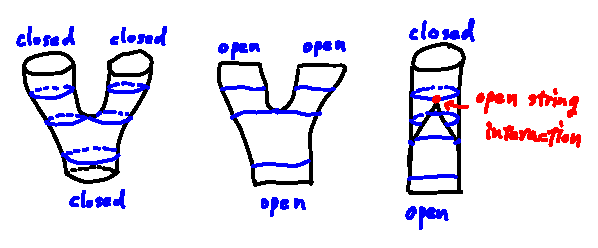
\includegraphics[width=350pt]{OpenClosed.eps}}
\caption{Open string interaction induces closed string}
\label{OpenClosed.eps}
\end{figure}

\subsubsection{Boundary conditions \& D-brane}

Let us consider an open string action.
\begin{align*}
 S_\mathrm{E} = \frac{1}{4\pi \alpha'} \int_{\sigma=0}^{\sigma=\pi} dtd\sigma
 \left( \partial_t X \cdot \partial_t X +\partial_\sigma X \cdot \partial_\sigma X  \right) \ ,
\end{align*}
where the subscript $E$ shows the world-sheet(WS) is Euclidean.
The variation principle leads
\begin{align*}
 0 &= \delta S
 = \frac{1}{2\pi \alpha'} \int_{\sigma=0}^{\sigma=\pi} dtd\sigma
 \left( \partial_t X \cdot \partial_t \delta X +\partial_\sigma X \cdot \partial_\sigma \delta X  \right)  \nonumber\\
 &= \frac{1}{2\pi \alpha'} \int_{\sigma=0}^{\sigma=\pi} dtd\sigma
 \left[ -\delta X \cdot \left( \partial_t \partial_t X +\partial_\sigma \partial_\sigma X \right)
 + \partial_t\left(\partial_t X \cdot \delta X \right) + \partial_\sigma \left( \partial_\sigma X \cdot\delta X \right)  \right]  \nonumber\\
 &= \frac{1}{2\pi \alpha'} \int dt \left[ \partial_\sigma X \cdot\delta X  \right]_{\sigma=0}^{\sigma=\pi} \ .
\end{align*}
At the last equality we used E.O.M and $\delta X (t=\pm \infty)=0$.
The equation compels us to impose one of either boundary conditions:
\begin{align*}
 \begin{array}{ll}
  \partial_\sigma X^\mu |_\mathrm{bdy} = 0 \qquad &\textrm{Neumann condition}  \\[4pt]
  \delta X^\mu |_\mathrm{bdy} = 0 \textrm{ or } X^\mu = c^\mu \ (\mathrm{const}) \qquad &\textrm{Dirichlet condition}
 \end{array}
\end{align*}


From the homework 1 we saw that the solution for Dirichlet boundary condition
express a momentum NON-conservation (see Fig.~\ref{BoundaryObj.eps}).
\begin{figure}[htb]
\centerline{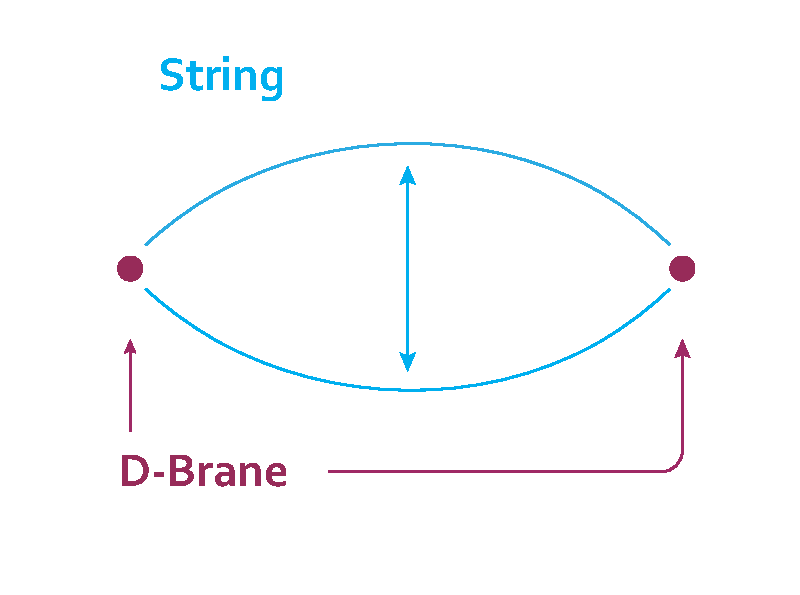
\includegraphics[width=100pt]{BoundaryObj.eps}}
\caption{D-brane must exist at the ends of open string so that momentum can escape from string.}
\label{BoundaryObj.eps}
\end{figure}
It implies that there must be something into which the momentum goes.
We call this object \textbf{D-brane}, where the D stands for Dirichlet and
brane comes from membrane.
D-brane is a dynamical object as it should receive the momentum,
hence, it has action and interactions with string.
On the other hand, in order to stay at a specific point $X^\mu = c^\mu$
D-brane must be infinitely heavy compared to string.


One can impose a certain number of Neumann condition and the rest is Dirichlet, let us set:
\begin{align*}
 &\textrm{Neumann condition on } X^a \quad (a=0,1,\ldots,p)  \\
 &\textrm{Dirichlet condition on } X^I \quad (I=p+1,\ldots,D-1)
\end{align*}
The corresponding D-brane is called D$p$-brane (e.g. D3-brane).
\textbf{D$p$-brane} is a spatially $p$-dim object and space-timely $(p+1)$-dim object.
Now we can visalize a configuration of D-brane and string as in Fig.~\ref{DpBrane.eps}.
\begin{figure}[htb]
\centerline{\includegraphics[width=150pt]{DpBrane.eps}}
\caption{Visalization of D$p$-brane and open string.}
\label{DpBrane.eps}
\end{figure}



\subsubsection{Chan-Paton factor}

We can consider not only a D-brane but many D-branes,
and a string now have an option on which D-brane a string ends.
Let us label this option $i$ ($i=1,\ldots,n$), which is called \textbf{Chan-Paton factor}.
As an open string has two end points a string state has two Chan-Paton degree:
\begin{align*}
 |N;k \rangle  \quad  \to \quad |N;k;ij \rangle \ .
\end{align*}
Now we have $n^2$ massless vector states in both bosonic- or super-string theory.
As usual we use $n \times n$ Hermite matrices $T^a$ normalized to
\begin{align*}
 \Tr (T^a T^b) = \delta^{ab} \ ,
\end{align*}
which is a complete set for the end points:
\begin{align*}
 |N;k;a \rangle = T^a_{ij} |N;k;ij \rangle \ .
\end{align*}
You will find this is $\U(n)$ gauge fields
if you compute a three point amplitude.



Note that in order to realize $\U(n)$ gauge group the D-branes must coincide at a point.
Otherwise, the gauge group is broken by Higgs mechanism (see Fig.~\ref{ManyD.eps}).
\begin{figure}[htb]
\centerline{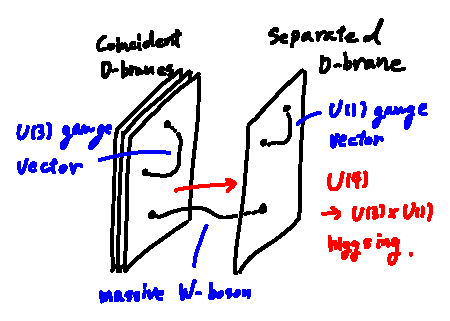
\includegraphics[width=250pt]{ManyD.eps}}
\caption{Many D-branes and Chan-Paton factors. $\U(n)$ gauge group and Higgs mechanism.}
\label{ManyD.eps}
\end{figure}


We will see, in next lectures, that other type of gauge groups ($SO$ or $Sp$) can be realized in string theory.



\subsubsection{D-brane in IIA/IIB superstring theory}


In the previous lecture note we saw that IIA/IIB superstring theory has RR fields,
which are anti-symmetric tensors and are analogy of gauge fields.
Furthermore, again from an analogy of electro-magnetic dynamics,
there are objects which electrically/magnetically coupled to the gauge fields
like an electron/monopole.
It is known that for RR fields such objects are D-branes.
In order to justify the statement we need more elaborated tools.
Here we simply see that which D$p$-branes couple to RR fields in IIA/IIB.


Let us start with an electron/monopole in 4-dim spacetime.
Electron is expressed by a source
$J^\mu = (\rho, \bfj) = (q \delta^3(\bfr-\bfr(t)), \partial_t \bfr(t) \rho )$
and its coupling to gauge field is written by
\begin{align*}
 S_J = q \int A_\mu J^\mu d^4x = q \int_C A_\mu dx^\mu = q \int_C A \ ,
\end{align*}
where $q$ is an electric charge, $C$ is a worldline of the electron, and $A$ is understood as 1-form.
Similarly, D$p$-brane ($p\le 3$) couples to $(p+1)$-tensor RR field as follows.
\begin{align*}
 S_{Dp} = \int_{M_{p+1}} C_{p+1} \ ,
\end{align*}
where $C_{p+1}$ is a $(p+1)$-form RR gauge potential
and $M_{p+1}$ is a world-membrane of D$p$-brane.
Note that an exteriror deribative of the potential
gives its field strength $G_{p+1} = d C_p$.
For example of D$3$-brane is:
\begin{align*}
 S_{D3} &= \int_{M_{4}} C_{4} = \frac{1}{4!} \int_{M_{4}} C_{\mu\nu\rho\sigma}
 dX^\mu \wedge dX^\nu \wedge dX^\rho \wedge dX^\sigma  \nonumber\\
 &= \frac{1}{4!} \int_{M_{4}} C_{\mu\nu\rho\sigma} \epsilon^{abcd}
 \frac{\partial X^\mu}{d\sigma^a} \frac{\partial X^\nu}{d\sigma^b}
 \frac{\partial X^\rho}{d\sigma^c} \frac{\partial X^\sigma}{d\sigma^d} d^4\sigma \ ,
\end{align*}
where $\sigma^a$ is a world-sheet coordinate of D$3$-brane and $X^\mu$
is an embeding of D$3$-brane into space-time.
The reason why it is limited up to $p=3$ is because
we only have up to $4$-tensor RR-field in IIA/IIB superstring theory.


% Monopole cannot be expressed by fundamental particle,
% rather it is a solitonic object, which is expressed by a field configuration.
Monopole is characterized by maginetic flux measured at surface surrounding the monopole
(see Fig.~\ref{mono.eps})
\begin{figure}[htb]
\centerline{\includegraphics[width=150pt]{mono.eps}}
\caption{Monopole is measured by magnetic flux configuration.}
\label{mono.eps}
\end{figure}
\begin{align*}
 q_m &= \int_S B \cdot n dS = \int_{B_3} \nabla \cdot B dV \ , \\
 &= \int_{\partial B} F_2 = \int_{B} dF_2 \ ,
\end{align*}
where $q_m$ is a magnetic charge, $B$ is magnetic flux, $S$ is a surface surrounding
the monopole, $B_3$ is a 3-dim ball, whose boundary is $S$,
$B$ in the second line is $B_3$, and $\partial B$ is a surface of $B$, which is $S$.
Note that $F_2$ cannot be expressed by an exterior derivative $dA$ globally,
hence, $dF_2 \neq 0$, rather $dF_2 = \nabla \cdot B = q_m \delta^3(r)$.
If we extend this idea to D$p$-brane ($p \ge 3$)
\begin{align*}
 q_m &= \int_{\partial B_{D-(p+1)}} G_{D-(p+2)} = \int_{B_{D-(p+1)}} dG_{D-(p+2)} \ .
\end{align*}
See Fig.~\ref{MagD.eps} to understand the direction of the flux $G_{D-(p+2)}$,
which leads potential $C_{D-(p+3)}$.
The reason why $p \ge 3$ is because $D=10$ and the highest tensor is $[4]$.
\begin{figure}[htb]
\centerline{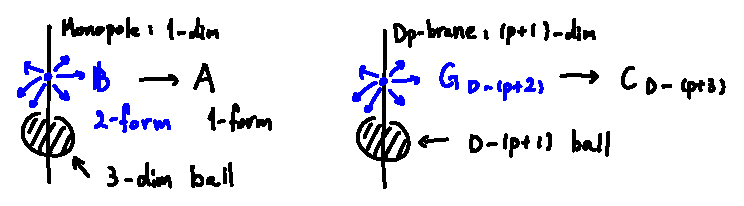
\includegraphics[width=350pt]{MagD.eps}}
\caption{Higher dimensional analog of monopole: magnetically coupled D$p$-brane.}
\label{MagD.eps}
\end{figure}

If you allow to use electro-magnetic duality it is more easily understood (see Fig.~\ref{EleMagD.eps}).
\begin{figure}[htb]
\centerline{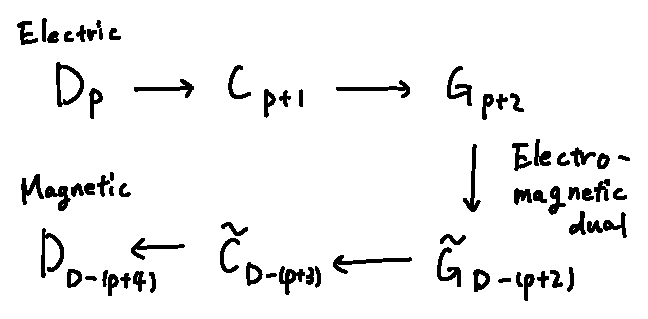
\includegraphics[width=250pt]{EleMagD.eps}}
\caption{Electro-magnetic duality and D-brane.}
\label{EleMagD.eps}
\end{figure}

String or fundamental string, denoted as F$1$, is electrically coupled to B-field.
On the other hand, there is an object that is magnetically coupled to B-field,
which is called \textbf{NS$5$-brane}.


Now you should notice that in IIA/IIB string theory the number $p$ of D$p$-brane
is limited to a certain number.
This is because the rank of RR-field (tensor) is limited.
Let us summarize which D-brane can exist in which superstring theory (see Table~\ref{table:001}).
\begin{table}[htbp]
 \centering{
  \caption{Possible D-branes in IIA/IIB superstring, fundamental string, and NS$5$-brane.}
  \vspace{4pt}
  \label{table:001}
\begin{tabular}{l|ccc}
  IIA & $B_2$ & $C_1$ & $C_3$ \\
\hline
  Electric & F$1$ & D$0$ & D$2$ \\
  Magnetic & NS$5$ & D$6$ & D$4$ \\
\end{tabular} \hspace{12pt}
\begin{tabular}{l|cccc}
  IIB & $B_2$ & $C_0$ & $C_2$ & $C_4^+$ \\
\hline
  Electric & F$1$ & D$(-1)$ & D$1$ & D$3$ \\
  Magnetic & NS$5$ & D$7$ & D$5$ & D$3$ \\
\end{tabular}
}
\end{table}
\vspace{2pt}
\noindent
\textbf{Comments:}\vspace{-2pt}
\begin{itemize}
 \item Only D$p$-brane for even $p$ exist in IIA and for odd $p$ in IIB.
 \item D$(-1)$-brane is timely localized object (like instanton).
 \item D$8$-brane can exist in IIA, which is a non-dynamical object
       and there is no corresponding anti-symmetric tensor.
\end{itemize}






\section{T-duality}


We have seen that the critical dimensions $D$ of bosonic and supersymmetric string theory are $D=26$ and $D=10$, respectively. To obtain an effective theory in lower dimensions, we can make use of \textbf{Kaluza-Klein compactifications} where  the 
true spacetime takes the form of a direct product $M_{d} \times K_{D-d}$, where 
$M_d$ is the $d$-dimensional Minkowski spacetime, and $K_{D-d}$ is a very tiny compact manifold. As we will see, an effective theory in $M_d$ still sees interesting ``stringy'' effects in this Kaluza-Klein scheme. 




First we concentrate on the simple compactifications, $K=T^{D-d}$
called \textrm{toroidal compactifications}.  Since a torus is simply a  product of $S^1$ and are flat,  the nonlinear sigma model can be described by the free two-dimensional CFT. Remarkably, this simple compactification leads to the notion of \textbf{T-duality} and \textbf{Heterotic string theories} have been constructed based on toroidal compactifications. To understand the basic properties,  let us first see study the toroidal compactifications of bosonic string theory. Toroidal compactifications of superstring theories are also very interesting so that we will learn them relating to string dualities later more in detail.


The concept of D-branes was introduced in the last lecture as boundary conditions of open strings. T-duality gets particularly rich when we include D-branes so that we will study their properties more in detail. 



\subsection{$S^1$ compactification in closed bosonic string}

To begin with, let us first study the simplest case of the spacetime $\bR^{1,24}\times S^1$ where we compactify 25-th direction on a circle $S^1$ of radius $R$.  For closed strings, we have the 
familiar mode expansion 
$X^\mu(z,\bz)=X^\mu(z)+\overline X^\mu(\bz)$ with
\begin{align}
X^\mu(z)&=x^\mu+i\sqrt{\ap\over2}
\left(-\alpha_0^\mu
\ln z+\sum_{m\neq0}{\alpha^\mu_m\over mz^m}\right), \nonumber\\
\overline X^\mu(\bz)&={\wt x}^\mu+i\sqrt{\frac{\ap}{2}}\left(-{\wt\alpha}_0^\mu
\ln \bz+\sum_{m\neq0}{{\wt\alpha}^\mu_m\over m\bz^m}\right).\nonumber
\end{align}
Now let us take a close look at the zero modes which can be written as
\be\nonumber
X^\mu(z,\bar{z}) = x^\mu + \wt x^\mu -i\sqrt{\a'\over2}
(\alpha^\mu_0+{\wt\alpha}^\mu_0)t + \sqrt{\a'\over2}
({\wt\alpha}^\mu_0-{\alpha}^\mu_0)\sigma
+ {\rm oscillators}.
\ee
where the spacetime momentum of the string is
\be\nonumber
p^\mu =
{1\over{\sqrt{2\a'}}}(\alpha^\mu_0 + {\wt\alpha}^\mu_0)~.
\ee

Under $\sigma \to \sigma+2\pi$,
the oscillator term are periodic and $X^\mu(z,\bar{z})$
changes by $2\pi\sqrt{(\a'/2)}(\wt\alpha^\mu_0-{\alpha}^\mu_0).$
For a non-compact spatial direction $\bR^{1,24}$, $X^\mu$ is single-valued $X^\mu(t,\s)= X^\mu(t,\s+2\pi)$,
which requires
\be\nonumber
\alpha^\mu_0={\wt\alpha}^\mu_0=\sqrt{\a'\over2}p^\mu~,\qquad \mu=0,1,\ldots,24~.
\ee

\begin{figure}[h]\centering
\includegraphics{winding}
\end{figure}


On the other hand, since the 25-th direction is put on the circle $S^1$ of radius $R$, it has period
 $X^{25}\sim X^{25}+2\pi R$. Hence, the momentum $p^{25}$ can take the values $n/R$ for $n\in\bZ$ where $n$ is called \textbf{Kaluza-Klein momentum}.
Also, under $\sigma\sim\sigma+2\pi$, $X^{25}(z,\bar{z})$
can change by $2\pi wR$ where $w$  is called 
 the \textbf{winding number}.  Thus, we have
\begin{align}\nonumber
\alpha^{25}_0+{\wt\alpha}^{25}_0 =
{2n\over R}\sqrt{\a'\over2} ~, \qquad
\wt\alpha^{25}_0-{\alpha}^{25}_0 = 
\sqrt{2 \over \a'}wR~,
\end{align}
implying
\begin{align}\label{25a}
\alpha^{25}_0 = \left({n\over R}-{wR\over\a'}\right)
\sqrt{\a'\over2} ~, \qquad
{\wt\alpha}^{25}_0 =
\left({n\over R}+{wR\over\a'}\right)\sqrt{\a'\over2}~.
\end{align}

Now let us study their mass spectrum. The mass formula for the string with one dimension compactified on a circle can be interpreted from a 25-dimensional viewpoint in which one regards each of the Kaluza-Klein momenta, which are given by $n$, as distinct particles. Thus, the mass formula is given by
$$M^2 = -\sum_{\mu=0}^{24}p^\mu p_\mu $$
where $\mu$ runs only over the non-compact dimensions.
Hence, we can write the mass formula as
$$
M^2 =
{2\over\a'}(\alpha_0^{25})^2+{4\over\a'}
({ N}-1) = {2\over\a'}({\wt\alpha}_0^{25})^2+{4\over\a'}
( {\wt N}-1).
$$
where $N$ and $\wt N$ are the right and left numbering operator (See lecture note 1). Using \eqref{25a}, we can express the difference of the two expression
\be\label{level-matching}
N-\wt N=nw~,
\ee
so that the level matching condition is modified due to the $S^1$ compactification. In a similar fashion, the mass can be expressed in terms of the Kaluza-Klein momentum and the winding number 
\be\label{mass}
M^2=\frac{n^2}{R^2}+\frac{w^2R^2}{\a'^2}+\frac2{\a'}(N+\wt N-2)
\ee




%As $R \to \infty$, all states with
%$w\neq 0$ become infinitely massive, while the $w=0$ states with all
%values of $n$ go over to a continuum.  As $R\to 0$, all states with $n
%\neq 0$ become infinitely massive.  In field theory this is all that would
%happen---the surviving fields would be independent of the compact
%coordinate, so the effective dimension is reduced.  In closed string theory
%things work quite differently: the $n=0$ states with all $w$ values form a
%continuum as $R\to 0$, because it is very cheap to wind around the small
%circle.  In the $R\to 0$ limit, the compactified dimension reappears!


The mass spectra \eqref{mass} of the theories at radius $R$ and $\a'/ R$ are identical
when the winding and Kaluza-Klein modes are interchanged
$n \leftrightarrow w$. This symmetry of the bosonic string theory is called \textbf{T-duality}.  This is the first and still most striking indication that strings see
spacetime geometry differently from the way we are used to.  Indeed, many
other examples of `stringy geometry' or `quantum geometry' are closely
related to this.



It is easy to see from \eqref{25a} that this interchange amounts to
\be\nonumber
\alpha^{25}_0 \rightarrow-\alpha^{25}_0, \quad
{\wt\alpha}_0^{25} \rightarrow {\wt\alpha}_0^{25} 
\label{tzemo}.
\ee
In fact, it is not just the zero mode, but the entire right-moving part of the compact coordinate that flips sign under the T-duality transformation
\be
X^{\prime25}(z,\bar{z})=-X^{25}(z)+\overline X^{25}(\bar{z})\ . \label{onesidep}
\ee
Remarkably, the energy-momentum tensor, OPEs and therefore all of the correlation
functions are invariant under this rewriting. In other words, T-duality, relating the two theories with radius $R$ and $\a'/R$, is an exact
symmetry of perturbative closed string theory.  

Because of the T-duality, a theory with compactification radius $R$ is equivalent to the theory with compactification radius $\a'/R$. Thus, this implies that there is a ``minimal radius'' $R=\sqrt{\a'}$ in string theory which is called \textbf{self-dual radius}. At self-dual radius, the duality
$R \to \a'/R$ maps $R$ back to its original value where we can expect 
something interesting to occur.  In the next section, we will study the physics at the self-dual radius.





\subsubsection{Self-dual radius: $R = \protect \sqrt {\a'}$}

As we know, the massless spectra of bosonic string theory includes graviton. Hence, let us see the effect of the $S^1$ compactification on the graviton. In the Kaluza-Klein mechanism  $M^{25}\times S^1$, the metric is decomposed into compact and non-compact spacetime direction
\be\label{KK-metric}
ds^2 = G_{MN} dx^M dx^N = G_{\mu\nu} dx^\mu dx^\nu + G_{25,25}(dx^{25}+ A_\mu dx^\mu)^2 ~.
\ee
where the fields $G_{\mu\nu}$, $G_{25,25}$, and $A_\mu$ are allowed to depend only on the non-compact coordinates $x^\mu$ ($\mu=0,1,\ldots24$). Under a coordinate transformation
$$x'^{25} = x^{25} + \lambda (x^\mu)  $$
the part $G_{\mu,25}=G_{25,\mu}$ of the metric transforms as
$$A'_\mu = A_\mu - \partial_\mu \lambda~ . $$
Thus, it behaves as $\U(1)$ gauge field, and gauge transformations arise as part of the higher-dimensional coordinate transformation. On the other hand, the part $G_{25,25}$ of the metric behaves as a scalar field. Indeed, writing $G_{25,25}=e^\s$, the Ricci scalar for the metric  \eqref{KK-metric} can be written as
$$
R_{26} = R_{25} - 2e^{-\s}\nabla^2 e^\s - \frac14e^{2\s}F_{\m\n}F^{\m\n}~ .
$$
Actually, it is straightforward to see the corresponding vertex operators at generic radius $R$:
\begin{align}	
\partial X^\mu \bar \partial X^\nu e^{i k\cdot X}	&\quad \longleftrightarrow \quad G_{\mu\nu}, B_{\mu\nu}, \phi \cr
\partial X^\mu \bar{\partial} X^{25} e^{i k\cdot X}, \ \partial X^{25} \bar{\partial} X^\mu e^{i k\cdot X}& \quad \longleftrightarrow \quad A^\mu\,,B_{\mu,25}\cr
\partial X^{25} \bar{\partial} X^{25} e^{i k\cdot X}&\quad \longleftrightarrow \quad  \sigma
\end{align}
where $\nu = 0, \ldots, 24$  runs the coordinate indices for $M_{25}$.  In fact, the middle line indicates that the theory has $\U(1)_\ell \times \U(1)_r$ gauge symmetry at generic radius $R$.

However, at the self-dual radius $R=\sqrt{\a'}$, the mass formula \eqref{mass} becomes
$$
M^2=\frac{1}{\a'}(n^2+w^2+2(N+\wt N-2))~,
$$
so that the massless spectra actually gets enlarged. In addition to the generic solution $n=w=0$, $N=\wt N =1$, there are now
also
\begin{table}[h]\centering
\begin{tabular}{ccccc}
&$n$&$w$&$\wt  N$&$N$\\\hline
A&$\pm1$&$\pm1$&$0$&$1$\\
B&$\pm1$&$\mp1$&$1$&$0$\\
C&$\pm2$&$0$&$0$&$0$\\
D&$0$&$\pm2$&$0$&$0$
\end{tabular}\end{table}

\noindent Hence, the states corresponding to A and B contain four new gauge bosons (A,B,C,D contain new massless scalars too that will appear in Homework 8), with vertex operators
$$
\bar{\partial} X^\mu e^{\pm 2iX^{25}(z)/\sqrt{\a'}} e^{i k\cdot X} ~,  \qquad\qquad  {\partial} X^\mu e^{\pm 2i\overline X^{25}(\bar z)/\sqrt{\a'}} e^{i k\cdot X}~.
$$
It is expected that the new gauge bosons must combine with the
old into a non-Abelian theory. In fact, if one can define the current 
$$
j^\pm(z)=j^1(z)\pm i \, j^2(z):=e^{\pm 2iX^{25}(z)/\sqrt{\a'}} \qquad j^3(z):=i\, \partial X^{25}(z)/\sqrt{\a'}~,
$$
they satisfy the OPEs (Exercise)
$$
j^a(z) j^b (0) \sim \frac { k\delta^{ab} } {2z^2}  
		+ \frac {i {\epsilon^{abc}} j^c(0)} {z}~.
$$
with $k=1$. Here $\epsilon^{abc}$ is the structure constant 
of $\SU(2)$.  This is precisely the definition of $\SU(2)$ affine Lie 
algebra with level $k=1$.  The same story is repeated for the left movers.  Hence we see that we have 
an enhancement of gauge symmetry from $\U(1)_\ell \times \U(1)_r$
to $\SU(2)_\ell \times \SU(2)_r$ at $R = \sqrt{\a'}$.


In fact, when the theory moves away from the self-dual radius $R=\sqrt{\a'}$, the $\SU(2)_\ell \times \SU(2)_r$  gauge symmetry is Higgsed. 
The world sheet action is deformed by turning on the marginal operator 
$$
V_{a\wt a}:=j_a \bar j_{\wt a} e^{ik\cdot X}~,
$$
which is equivalent to giving the VEV of the $(3,3)$-component of Higgs filed. As a result, when the theory is away from the self-dual 
radius, the $\SU(2)_\ell \times \SU(2)_r$ 
gauge symmetry is spontaneously 
broken down to a $\U(1)_\ell \times \U(1)_r$.



\subsection{T-duality of Open Strings}


Now let us consider the open string spectrum in the $S^1$ compactification.  Open strings with Neumann boundary conditions have no   wind number around the periodic dimension; they have no quantum
number comparable to $w$.  So when $R \to 0$ the states with nonzero
momentum go to infinite mass, but there is no new continuum of states.
This looks contrary to the case of closed strings.

Indeed, the remedy follows from the duality
transformation~(\ref{onesidep}) under which the Neumann condition is exchanged the Dirichlet
condition:
$$
\partial_\sigma X^{25} \Big|_{\sigma=0,\pi}=0 \quad \to\quad \partial_t X'^{25} \Big|_{\sigma=0,\pi}=0~.
$$
Consequently, 
the $X^{25}$ coordinate of the open string endpoints is fixed after T-duality, so the endpoint is constrained
to lie on a D-brane. Hence, T-dualities with open strings always involve D-branes. To see this, integrate 
\begin{align}
X'^{25}(\pi) - X'^{25}(0) &= \int_0^\pi d\sigma \partial_\sigma X'^{25}
\ =\ i \int_0^\pi d\sigma \partial_t X^{25} \nonumber\\
&= 2\pi \a' p^{25}\ =\ \frac{2\pi \a' n}{R}\ =\ 2\pi n R'. \label{deltax}
\end{align}
Here the KK momentum $n$ is transformed to winding number $n$  as in figure.
\begin{figure}[h]\centering
\includegraphics[width=13cm]{open-T-duality}
\end{figure}
For two different open strings, consider the connected world-sheet that
results from graviton exchange between them.  One can carry out the same
argument~(\ref{deltax}) on a path connecting any two endpoints, so all
endpoints lie on the same D-brane.  The ends are still free to move in
the other $D-2 = 24$ spatial dimensions.

In the previous lecture, we learnt that D-branes are associated to 
Chan-Paton factors. Now let us see how the Chan-Paton factors arise in this setting.
Open strings give rise to gauge fields and we now consider $\U(N)$ spacetime gauge fields. If  the
$X^{25}$ direction is compactified on the circle $S^1$, we can include a Wilson line $A_{25}={\rm
diag}\{\theta_1,\theta_2,\ldots,\theta_N\}/2\pi R$ on  $S^1$. The presence of the Wilson line 
generically breaking $\U(N) \to \U(1)^N$, which can be locally written in pure gauge:
\be\nonumber
A_{25} = -i\Lambda^{-1}\partial_{25}\Lambda,\qquad
\Lambda={\rm diag}\{e^{ i X^{25}\theta_1/2\pi R},e^{ i X^{25}\theta_2/2\pi
R}, \ldots , e^{ i X^{25}\theta_N/2\pi R} \}\ .
\ee
Then, the open string momenta is now shifted by
\be
{\rm diag}\left\{ e^{-i\theta_1}, e^{-i\theta_2}, \ldots, e^{-i\theta_N}
\right\} \nonumber
\ee
  Since the momentum is dual to the winding number, we
expect the fields in the dual description to have fractional winding
number, meaning that their endpoints are no longer on the same D-brane.  Indeed,
a string whose endpoints are in the state $|ij\rangle$ picks up a phase
$e^{i(\theta_j - \theta_i)}$, so the momentum is $(2\pi n + \theta_j -
\theta_i)/2\pi R$.  The calculation~(\ref{deltax}) then gives
\be\nonumber
X'^{25}(\pi) - X'^{25}(0) = (2\pi n + \theta_j - \theta_i) R'.
\ee
In other words, up to an arbitrary additive normalization, the endpoint in
state $i$ is at 
\be
X'^{25}\ =\ \theta_i R' \ =\ 2\pi\a' A_{25,ii}. \nonumber
\ee  
There are in general $N$
D-branes at different positions as schematically depicted in the following figure.
\begin{figure}[h]\centering
\includegraphics[width=7cm]{open-Higgs}
\end{figure}

\noindent Then, the $D-1$ dimensional mass of this open string is
\begin{align}
M^2 &= (p^{25})^2+{1\over\a'}({N}-1) \nonumber\\
&= \left( {[2\pi n+(\theta_j-\theta_i)]R^\prime\over2\pi\a'}
\right)^2 +{1\over\a'}(N-1).\nonumber
\end{align}
Note that $[2\pi
n+(\theta_i-\theta_j)]R^\prime$ is the minimum length of a string winding
between D-branes $i$ and $j$.  Massless states arise
generically only for non-winding open strings whose end points are on the
same D-branes, as the string tension contributes an energy to a stretched
string. 
We have therefore the massless states and the corresponding vertex operators
\begin{align}\nonumber
\alpha^{\mu}_{-1}|{ k};ii\rangle, &\quad\longleftrightarrow\quad  \partial_t X^\mu e^{ik\cdot X}, \cr
\alpha^{25}_{-1}|{ k};ii\rangle, &\quad\longleftrightarrow\quad \partial_t X^{25}e^{ik\cdot X} = \partial_\sigma
X'^{25}e^{ik\cdot X}~.
\end{align}

The first of these is a gauge field
living on the D-brane, with $24+1$ components tangent to the D-brane. 
The second was the gauge field in the compact direction in the original
theory.  In the dual theory it becomes the transverse position of the
D-brane.  

More generally, boundary condition of open strings can be of arbitrary dimensions. Since T-duality interchanges N and D boundary conditions, a
further T-duality in a direction tangent to a D$p$-brane reduces it to a
D$(p-1)$-brane, while a T-duality in a direction orthogonal turns it into a
D$(p+1)$-brane.  



In addition, let us make an important remark. So far, we have treat D-branes just as rigid boundary conditions. However, 
 D-branes are dynamical so that they can fluctuate in shape and position. As we will see in the subsequent lectures (hopefully!), the gravitational and gauge dynamics on a stack of D-branes makes string theory very intriguing. 




\subsection{T-duality of Type II Superstrings}
To end this lecture, let us briefly discuss how the 
T-duality 
 acts on Type II superstring compactified on $M^9 \times S^1$. We have seen that the T-duality acts as the parity transformation on the right-moving sector
 $$
  {X}^9 ( z)\quad\longleftrightarrow\quad -  {{X}'^9}( z)
 $$
The superconformal invariance requires 
$$\psi^9 \leftrightarrow - {\psi}^{'9}~.$$
 However, this implies that the chirality of the right-moving R sector ground state is reversed: the raising and lowering operators ${\psi}^{'8}±\pm i{\psi}^{'9}$ are interchanged. In other words, T-duality is a spacetime parity operation on just one side of the world-sheet, and so reverses the relative chiralities of the right- and left-moving ground states. As a result, Type IIA theory with compactification radius $R$ is T-dualized to Type IIB theory with radius $\a'/R$.
 

Since the IIA and IIB theories have different R-R fields, T-duality in the 9th direction
must transform one set into the other.  The action of duality on the spin
fields is of the form
\be\nonumber
\psi^R_{\alpha} (z) \to  \beta_9 \psi^R_{\alpha} (z),\qquad
\overline\psi^L_{\alpha} (\bar{z}) \to\overline\psi^L_{\alpha} (\bar{z}) 
\ee
for $\beta_9 =\Gamma^9\Gamma^{11}$, the parity transformation (9-reflection) on the
spinors.  Since the RR vertex
operators are written as
$$
\overline\psi^L\G^{\mu_1\cdots \mu_p}{\psi^R}
~,
$$
Hence, the RR fields are transformed as
\begin{align}\nonumber
C_9 &\quad \to\quad C \cr
C_{\mu},C_{\mu \nu 9}&\quad \to\quad C_{\mu 9}, C_{\mu\nu}\cr
C_{\mu \nu \lambda}&\quad \to\quad C_{\mu \nu \lambda 9}~.
\end{align}




\section{Type I superstring theory}

What we will learn:
\vspace{-4pt}
\begin{itemize}
 \setlength{\itemsep}{0pt}
 \item Type I superstring theory.
 \item In Type I theory, we only have D$1$-, D$5$-, and D$9$-, branes.
 \item O$9^-$-plane is needed for Type I to be consistent theory.
 \item T-duality of Type I theory.
\end{itemize}
\vspace{-4pt}


So far, we have learnt two kinds of superstring theory, which are Type IIA and IIB.
Both of them are closed superstring theory.
Note that we also learnt about D-branes in Type II theories, which leads open string.
However, note that we are considering a situation in which there exist D-branes,
so it is not a theory.


Actually, an open string cannot exist in Type II theories (without D-branes),
due to supersymmetry as follows.
After GSO projection an open string can have one of the following massless states:
\begin{align*}
 &P_\mathrm{GSO}: \quad \mathrm{NS+}, \ \mathrm{R+} = \textbf{8}_v +\textbf{8}_s \ ,  \\
 &\wt P_\mathrm{GSO}: \quad \mathrm{NS+}, \ \mathrm{R-} = \textbf{8}_v +\textbf{8}_c \ ,
\end{align*}
where $\textbf{8}_v$ is a space-time vector field and $\textbf{8}_{s,c}$ are gauginos.
$\mathcal N=2$ supersymmetry requires for $\textbf{8}_v$ to have two superpartners
as like for a graviton to have two gravitinos.
However, as you see, the gauge field has only one superpertner,
and hence, cannot exist in Type II theories.


The existence of (parallel) D-branes, as you might notice,
breaks the half of supersymmetries,
and hence, an open string can exist in such a situation.



The world-sheets(WS) we have considered are oriented ones.
However, it is quite natural to consider processes in Fig.~\ref{unorientedWS.eps}.
\begin{figure}[htb]
 \centerline{\includegraphics[width=200pt]{unorientedWS.eps}}
\caption{Unoriented processes. The left is open string one, and the right is closed string one.}
\label{unorientedWS.eps}
\end{figure}
Therefore, we will consider so called \textbf{unoriented string} in this lecture,
which leads Type I superstring theory.
%, which necessarily have an open string in the spectrum.
Argument below is almost in bosonic string, for simplicity, but it is straightfoward to apply for superstring.



\subsubsection{Orientation flip operation}

As the name indicates the orientation flip is nothing but an exchange of
left-/right-mover for closed string and a reversal of the direction for open string.


\noindent
\textbf{Closed string}

Let us define an orientation flip operator $\Omega$ for bosonic string, which flips the orientation of an closed string:
\begin{align*}
 \Omega :
 \begin{cases}
  X(t,\sigma) &\leftrightarrow \quad X(t,-\sigma) \\
  b(t,\sigma) &\leftrightarrow \quad \ol b(t,-\sigma)  \\
  c(t,\sigma) &\leftrightarrow \quad -\ol c(t,-\sigma)  \\
 \end{cases} \ ,
\end{align*}
where $t$ is the Eculideanized WS time, not $\tau$
(though there is no special meaning on it at this point).
Or, the operator acts on the modes as
\begin{align*}
 \Omega :
 \begin{cases}
  \alpha^\mu_n &\leftrightarrow \quad \wt \alpha^\mu_n \\
  b_n &\leftrightarrow \quad \ol b_n  \\
  c_n &\leftrightarrow \quad \ol c_n  \\
 \end{cases} \ ,
\end{align*}
where the modes are
\begin{align*}
 X(t,\sigma) &= x^\mu -i\alpha'p^\mu t +i\sqrt{\frac{\alpha'}{2}}
 \sum_{n \neq 0} \frac{1}{n} \left( \alpha^\mu_n e^{n(-t+i\sigma)} +
 \wt \alpha^\mu_n e^{n(-t-i\sigma)} \right) \ , \\
 b(t,\sigma) &= -\sum_{n \in \ZZ} b_n e^{n(-t+i\sigma)} \ , \quad
 \ol b(t,\sigma) = -\sum_{n \in \ZZ} \ol b_n e^{n(-t-i\sigma)} \ , \\
 c(t,\sigma) &= i\sum_{n \in \ZZ} c_n e^{n(-t+i\sigma)} \ , \quad
 \ol c(t,\sigma) = -i\sum_{n \in \ZZ} \ol c_n e^{n(-t-i\sigma)} \ ,
\end{align*}
where we can also use $w = -it -\sigma \leftarrow \tau -\sigma$ ($z = e^{iw}$).

We keep only $\Omega$ invariant states:\\[2pt]
\centerline{
\begin{tabular}{lll}
 OK & Tachyon & $|k\rangle$  \\[2pt]
 OK & Dilaton & $\alpha_{-1}\cdot \wt \alpha_{-1}|k\rangle$  \\[2pt]
 NG & B-field & $\alpha_{-1}^{[\mu} \wt \alpha_{-1}^{\nu]} |k\rangle$  \\[2pt]
 OK & Graviton & $\left(\alpha_{-1}^{(\mu} \wt \alpha_{-1}^{\nu)}
         -\frac{\delta^{\mu\nu}}{D}\alpha_{-1}\cdot \wt \alpha_{-1}\right) |k\rangle$  \\[2pt]
 & \hspace{12pt} $\vdots$ &
\end{tabular}
}\\
No B-field means that a closed string, which is electrically coupled to B-fields,
is not a stable object and should decay.
% With the remaining states we can consider an amplitude including unorientable world-sheet, such as a Klein bottle.




\noindent
\textbf{Open string}

Let us put a D$25$-brane and consider Neumann boundary conditions.
Then similarly, we define the orientation flip operator for open string:
\begin{align*}
 \Omega :
 \begin{cases}
  X(t,\sigma) &\leftrightarrow \quad X(t,\pi-\sigma) \\
  b(t,\sigma) &\leftrightarrow \quad \ol b(t,\pi-\sigma)  \\
  c(t,\sigma) &\leftrightarrow \quad -\ol c(t,\pi-\sigma)  \\
 \end{cases} \ ,
\end{align*}
or, for the modes expansion
\begin{align*}
 \Omega :
 \begin{cases}
  \alpha^\mu_n &\leftrightarrow \quad (-1)^n \alpha^\mu_n \\
  b_n &\leftrightarrow \quad (-1)^n b_n  \\
  c_n &\leftrightarrow \quad (-1)^n c_n  \\
 \end{cases} \ ,
\end{align*}
where the modes are
\begin{align*}
 X(t,\sigma) &= x^\mu -2i\alpha'p^\mu t +i\sqrt{\frac{\alpha'}{2}}
 \sum_{n \neq 0} \frac{\alpha^\mu_n}{n} \left( e^{n(-t+i\sigma)}
 +e^{n(-t-i\sigma)} \right) \ , \\
 b(t,\sigma) &= -\sum_{n \in \ZZ} b_n e^{n(-t+i\sigma)} \ , \quad
 \ol b(t,\sigma) = -\sum_{n \in \ZZ} b_n e^{n(-t-i\sigma)} \ , \\
 c(t,\sigma) &= i\sum_{n \in \ZZ} c_n e^{n(-t+i\sigma)} \ , \quad
 \ol c(t,\sigma) = -i\sum_{n \in \ZZ} c_n e^{n(-t-i\sigma)} \ .
\end{align*}


Naively, the massless vector field state is $\Omega$ variant.
However, we can keep the state by using Chan-Paton factor:
\begin{align*}
 |\Phi;\Lambda\rangle \equiv |\Phi;ij\rangle \Lambda_{ij} \ .
\end{align*}
When the orientation flips, the Chan-Paton indices are exchanged, so
\begin{align*}
 \Omega |\Phi;\Lambda\rangle = |\Omega\Phi;\Lambda^T\rangle \ .
\end{align*}
Therefore, $\Omega$ invariant states are\\[2pt]
\centerline{
\begin{tabular}{lll}
 Tachyon & $|k;\Lambda \rangle$ & $\Lambda^T = \Lambda$ \\[2pt]
 Vector & $\alpha_{-1}^\mu |k;\Lambda \rangle$ & $\Lambda^T = -\Lambda$ \\[2pt]
 \hspace{12pt} $\vdots$ &
\end{tabular}
}\\
The $n\times n$ hermitian, anti-symmetric matrix forms a $\SO(n)$ algebra.
Therefore, the vector field is identified with a $\SO(n)$ gauge field.


When we flip the orientation there could be a shuffle of the Chan-Paton
index because the D-branes are coincident.
Let us denote this as follows.
\begin{align*}
 &\Omega |\Phi;ij\rangle = |\Omega\Phi;kl\rangle P_{kj} P^{-1}_{il}
 \quad (P \in \U(n)) \ ,  \\
 &\Omega |\Phi;\Lambda\rangle = |\Omega\Phi;P\Lambda^T P^{-1}\rangle \ .
\end{align*}
There is a natural constraint $\Omega^2=1$,
and equivalence relation: $\Lambda \sim \wt\Lambda = U\Lambda U^{-1}$ $(U\in \U(n))$.
The constraint leads
\begin{align*}
 &\Omega^2 |\Phi;\Lambda\rangle = \Omega|\Omega\Phi;P\Lambda^T P^{-1}\rangle
 = |\Phi;P(P\Lambda^T P^{-1})^TP^{-1}\rangle \ ,  \\
 &\therefore \qquad \Lambda = PP^{-T} \Lambda (PP^{-T})^{-1} \ .
\end{align*}
For general $\Lambda$ to satisfy the relation above we need $PP^{-T} = 1$.
Since the order of the index is artificial, physics is invariant under the re-labelling,
$\Lambda \sim \wt\Lambda = U\Lambda U^{-1}$, and this leads the equivalence class for $P$ as well:
\begin{align*}
 P\Lambda^T P^{-1} = P(U^{-1}\wt \Lambda U)^T P^{-1} = P U^T \wt \Lambda^T U^{-T} P^{-1}
 = U^{-1} (U P U^T) \wt \Lambda^T (U P U^{T})^{-1} U \ .
\end{align*}
Thus, $\wt P \sim U P U^T$.
Subject to the constraint and the equivalence class,
we have two physically inequivalent choice for $P$:
\begin{itemize}
 \item $P = 1 \qquad \Lambda^T = -\Lambda \qquad \cdots$ $\SO(n)$ gauge symmetry.
 \item $P = i
       \begin{pmatrix}
        0 & -\textbf{1}_{k\times k}  \\
        \textbf{1}_{k\times k} & 0
       \end{pmatrix} 
       \qquad (n=2k)$ \\ $\qquad \Lambda^T = \begin{pmatrix}
        0 & -\textbf{1}_{k\times k}  \\
        \textbf{1}_{k\times k} & 0
       \end{pmatrix}\Lambda\begin{pmatrix}
        0 & -\textbf{1}_{k\times k}  \\
        \textbf{1}_{k\times k} & 0
       \end{pmatrix} \qquad \cdots$ $\Sp(n)$ gauge symmetry.
\end{itemize}



\noindent
\textbf{Unoriented superstring spectrum}

The orientation flip is a swap of left- and right-mover,
therefore, IIB theory has the world-sheet parity $\Omega$ because
it is a non-chiral theory.
The flip projection eliminates B-field $[2]$ in NS-NS sector,
as well as half of NS-R R-NS sector $\textbf{8}_c + \textbf{56}_s$ (only diagonal part survive).
Supersymmetry requires that the number of bosons and fermions are the same,
which implies that $[0]$ and $[4]_+$ are eliminated
and only the second rank anti-symmetric field $[2]$ survives in R-R sector.
The remaining states are
\begin{align*}
 [0] + [2] + (2) +\textbf{8}_c +\textbf{56} &= \textbf{1} +\textbf{28} +\textbf{35} +\textbf{8}_c +\textbf{56}_s  \cr
 &= \Phi +C_{\mu\nu} +G_{\mu\nu} +\lambda^- +\psi_\mu^+ \ .
\end{align*}
Absence of the $C$ and $C_{\mu\nu\rho\sigma}^+$ means that
there is no D$(-1)$-, D$3$-, D$7$-branes in Type I theory.
\textbf{Only D$1$-, D$5$-, D$9$-branes exist in Type I theory},
as the first two D-branes are electrically and magnetically coupled to
$C_{\mu\nu}$, respectively.
D$9$ is space-filling and non-dynamical, and is necessary to have an open string.
Actually, this Type I closed superstring theory is inconsistent as we will see,
and it necessarily includes open string $\textbf{8}_v +\textbf{8}_s$
(choice of the GSO projection follows from IIB).
Therefore, the spectrum of Type I theory (unoriented, open plus closed supersting)
is as follows.
\begin{align*}
  [0] + [2] + (2) +\textbf{8}_c +\textbf{56} +(\textbf{8}_v +\textbf{8}_s)_{SO(n) \textrm{ or } \Sp(n)} \ .
\end{align*}
Anomaly or tadpole cancellation argument, which we will see in the following subsection,
shows that \textbf{only $\SO(32)$ is consistent}.



% \begin{table}[htbp]
%  \begin{center}
%   \caption{}
%   \vspace{4pt}
%   \label{table:001}
% \begin{tabular}{|c|c|c|c|c|}
% \hline
% \hline
%   Category & Sector & $(h_A,h_B,h_T)$ & Mirror theory & ABJM model \\
% \hline
%  1 & & \parbox{40pt}{$(0,0,0)$ $(1,1,1)$} & $1.11906$ & $1.13290$ \\
% \hline
%  2 & & \parbox{40pt}{$(0,0,1)$ $(1,1,0)$} & $-0.10861$ & $-0.10861$ \\
% \hline
%  \multirow{2}{*}{\vspace{-15pt}3} & 3-1 & \parbox{40pt}{$(0,1,0)$ $(1,0,1)$} & $0.176777$ &
%  \multirow{2}{*}{\vspace{-15pt}$0.176577$} \\
% \cline{2-4}
%  & 3-2 & \parbox{40pt}{$(1,0,0)$ $(0,1,1)$} & $0.176777$ & \\
% \hline
% \hline
% \end{tabular}
% \end{center}
% \end{table}




\subsubsection{Amplitude of Type I theory}


As we saw in the previous subsection unoriented open string has
a $\SO(n)$ or $\Sp(n)$ massless gauge field.
However, all of them are anomalous, which means that the theories are inconsistent,
except $\SO(32)$ as we will see below.
There are a few ways to see the anomaly.
We utilize vacuum amplitudes.


First, let us consider ``oriented'' open string amplitude, whose WS is cylinder(=annulus), see Fig.~\ref{cylinder.eps}.
\begin{figure}[htb]
\centerline{\includegraphics[width=200pt]{cylinder.eps}}
\caption{Cylinder.}
\label{cylinder.eps}
\end{figure}
It is clear from the picture that
\vspace{-4pt}
\begin{itemize}
% \setlength{\parskip}{0cm}
 \setlength{\itemsep}{0pt}
 \item The range is $0 \le \Re w \le \pi$, the period is $w \sim w +2\pi il$.
 \item There is a real modulus $l$; the amplitude needs a $b$ zero mode insertion.
 \item There is a real isometry, shift of $\Im w$; the amplitude needs a $c$ zero mode insertion.
\end{itemize}
The cylinder partition function is
\begin{align*}
 A_{0,C} = \int \frac{dl}{2l} \langle b_0 c_0 \rangle_\mathrm{gh} \langle 1 \rangle_\mathrm{mat} \ ,
\end{align*}
where
\begin{align*}
 &b_0 = \frac{1}{2\pi} \int_0^{\pi} \left[ dw\ b(w) +d\ol w\ \ol b(\ol w)\right] \ , \\
 &c_0 = \frac{i}{2\pi} \int_0^{\pi} \left[ dw\ c(w) -d\ol w\ \ol c(\ol w)\right] \ .
\end{align*}
Assume that there are $n$ D$25$- (or D$9$- for superstring) branes so that all of the boundary condition is Neumann.
Using operator formalism we can derive each contributions as follows.
\begin{align*}
 \langle 1 \rangle_\mathrm{mat} &= n^2\ \Tr \left[ q^{L_0 -\frac{c}{24}} \right]
 \qquad (q=e^{-2\pi l}\ , \ L_0 = \alpha' p^2 +\sum_{n=1}^\infty \alpha_{-n}\cdot \alpha_{n})  \cr
 &= n^2 \cdot \frac{iV_{26}}{(2\pi)^{26}} (2l\alpha')^{-13} \cdot \eta(il)^{-26} \ .  \\
 \langle b_0 c_0 \rangle_\mathrm{gh} &= \Tr \left[ (-1)^F b_0 c_0 q^{L_0-\frac{c}{24}} \right] = \eta(il)^2
 \qquad (L_0 = \sum_{n \in \ZZ} n \nord{b_{-n}c_{n}}-1) \ .
\end{align*}
Therefore, the amplitude is
\begin{align*}
 A_{0,C} = n^2 \cdot \frac{iV_{26}}{(2\pi \ell_s)^{26}}\int_0^\infty \frac{dl}{2l} \frac{1}{(2l)^{13} \eta(il)^{24}} \ ,
\end{align*}
where $\ell_s = \sqrt{\alpha'}$ is the string length.
Let us look into the physical information that can be read off from the amplitude.
\vspace{-4pt}
\begin{itemize}
 \setlength{\itemsep}{0pt}
 \item UV divergence: there is a UV divergence from $l \to 0$, as opposed to the closed string case.
 \item Open string short 1-loop = closed string long propagation (see Fig.~\ref{openClosedAmp.eps}).\\
       \begin{figure}[htb]
        \centerline{\includegraphics[width=150pt]{openClosedAmp.eps}}
        \caption{Pictorical ``proof'' of the equivalence between open string 1-loop and closed string propagation.}
        \label{openClosedAmp.eps}
       \end{figure}
       This is justified by rewriting the amplitude. Using $\eta(il) = l^{-\frac{1}{2}} \eta(il^{-1})$
       we have
 \begin{align*}
  &A_{0,C} = \frac{n^2}{2^{14}} \cdot \frac{iV_{26}}{(2\pi \ell_s)^{26}} \int_0^\infty ds\ \eta(is)^{-24} \ ,  \\
  &\qquad \textrm{where} \quad \eta(is)^{-24} = q^{-1} +24 +\cdots \equiv \sum_{N=0}^\infty \mathcal N_N q^{N-1} \quad (q = e^{-2\pi s}) \ .
 \end{align*}
       Compare with the torus partition function (exercise).
 \item The UV divergence $l\to 0$ is replaced by IR divergence $s \to \infty$ of a closed string propagation,
       which can be understood particle propagations (sum of lines) as follows (see also Fig.~\ref{masslessProp.eps}).
       \begin{figure}[htb]
        \centerline{\includegraphics[width=150pt]{masslessProp.eps}}
        \caption{Intermediate propagation is replaced by particles(lines).}
        \label{masslessProp.eps}
       \end{figure}
 \begin{align*}
  \int_0^\infty ds \sum_{N=0}^\infty \mathcal N_N e^{-2\pi s(N-1)}
  \sim \left. \sum_{i} \int_0^\infty ds\ e^{-s(k^2+m^2_i)} \right|_{k=0} = \left. \sum_i \frac{1}{k^2+m^2_i} \right|_{k=0} \ .
 \end{align*}
       We can see that the IR divergence is from massless particle propagation (graviton etc.),
       which is absorbed or emitted from D$25$-branes.
 \item In conclusion, the divergence is due to the existence of the D$25$-branes,
       which has definite tension (this is why they emit graviton/dilaton).
       Can this not be eliminated ?? $\to$ unoriented string.
\end{itemize}



\noindent
\textbf{Klein bottle amplitude}

Next, let us consider a Klein bottle for WS and compute the amplitude on it.
As the Klein bottle can be realized by orientation flip operator as in Fig.~\ref{KleinBottle.eps}
\begin{figure}[htb]
\centerline{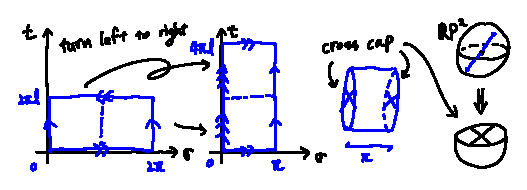
\includegraphics[width=350pt]{KleinBottle.eps}}
\caption{Klein bottle. It can be described by a cylinder with cross cap boundary on both ends.}
\label{KleinBottle.eps}
\end{figure}
it should be
\begin{align*}
 A_{0,K} = \frac{1}{2} \int \frac{dl}{2l}
 \Tr \left[ \Omega (-1)^F \frac{1}{2}(b_0+\ol b_0) \frac{1}{2}(c_0+\ol c_0) q^{L_0 +\ol L_0 -\frac{c}{12}} \right] \qquad (q=e^{-2\pi l}) \ ,
\end{align*}
where the factor of $\frac{1}{2}$ is from the projection operator $\frac{1+\Omega}{2}$,
or you can also regard it as an additional gauge redundancy $w \to \ol w$.



One can rewrite the amplitude as follows.
\begin{align*}
 A_{0,K} = \frac{1}{2} \int \frac{dl}{2l}
 \Tr \left[ (-1)^F b_0 c_0 q^{2L_0  -\frac{c}{12}} \right] \ ,
\end{align*}
where $c = c_\mathrm{mat} +c_\mathrm{gs} = 0$, and 
\begin{align*}
 L_0 = \frac{\alpha'}{4} p^2 +\sum_{n=1}^\infty \left( \alpha_{-n}\cdot \alpha_{n} +n b_{-n} c_n +n c_{-n} b_n \right) -1 \ .
\end{align*}
Thus, the result is
\begin{align*}
 A_{0,K} &= \frac{iV_{26}}{(2\pi \ell_s)^{26}} \int \frac{dl}{4l} \frac{1}{l^{13} \eta(2il)^{24}} \ , \\
 &= 2^{13} \frac{iV_{26}}{(2\pi \ell_s)^{26}} \int \frac{ds}{4} \eta(is)^{-24} \ .
\end{align*}




\noindent
\textbf{M\"obius strip amplitude}


Finally, let us consider a M\"obius strip for WS (see Fig.~\ref{MobiusStrip.eps}).
\begin{figure}[htb]
\centerline{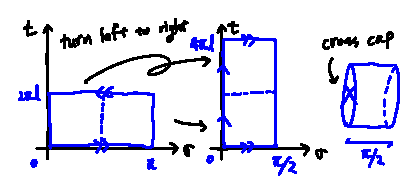
\includegraphics[width=300pt]{MobiusStrip.eps}}
\caption{M\"obius strip.}
\label{MobiusStrip.eps}
\end{figure}
It has
\vspace{-4pt}
\begin{itemize}
% \setlength{\parskip}{0cm}
 \setlength{\itemsep}{0pt}
 \item The range is $0 \le \sigma \le \pi$, the period is $2\pi l$, coming together with the orientation flip:
       $(t,\sigma) \sim (t+2\pi l,\pi -\sigma)$.
 \item There is a real modulus $l$; the amplitude needs a $b$ zero mode insertion.
 \item There is a real isometry, shift of $t$; the amplitude needs a $c$ zero mode insertion.
\end{itemize}

The M\"obius strip amplitude is
\begin{align*}
 A_{0,M} = \frac{1}{2} \int \frac{dl}{2l}
 \Tr \left[ \Omega (-1)^F b_0 c_0 q^{L_0 -\frac{c}{12}} \right] \qquad (q=e^{-2\pi l}) \ .
\end{align*}
The trace is over Hilbert space of the matter and ghost sectors on the strip
as well as the Chan-Paton index, which gives in total $n^2$ degeneracy for each state.
We can divide the effect of $\Omega$ into two parts as follows.
\begin{align*}
 \Omega |\Phi;\Lambda\rangle = |\Omega\Phi;P\Lambda^TP \rangle
 \equiv \Omega_\Phi \cdot \Omega_\Lambda |\Phi;\Lambda\rangle \ .
\end{align*}
Let us see the $\Omega_\Lambda$, which is defined as
\begin{align*}
 \Omega_\Lambda = \frac{P\Lambda^TP}{\Lambda} \ .
\end{align*}
In the case of $\SO(n)$, which means $P=1$,
\begin{align*}
 \Omega_{\Lambda,SO} = \frac{\Lambda^T}{\Lambda} =
 \begin{cases}
  +1 \qquad (\textrm{for symmetric $\Lambda$})  \\
  -1 \qquad (\textrm{for anti-symmetric $\Lambda$})
 \end{cases} \ ,
\end{align*}
Therefore,
\begin{align*}
 \Tr_{\Lambda,SO} \left[ \Omega \right] = \frac{n(n+1)}{2} -\frac{n(n-1)}{2} = n \ .
\end{align*}
In the case of $\Sp(n)$ (exercise)
\begin{align*}
 \Tr_{\Lambda,Sp} \left[ \Omega \right] = -n \ .
\end{align*}
The matter and ghost part is
\begin{align*}
 \Tr_\Phi \left[ \Omega (-1)^F b_0 c_0 q^{L_0 -\frac{c}{12}} \right]
 &= \frac{iV_{26}}{(2\pi \ell_s)^{26}} \frac{1}{(2l)^{13}}
 \cdot q^{-1} \prod_{n=1}^\infty \frac{(1-(-q)^n)^2}{(1-(-q)^n)^{26}}  \cr
 &= \frac{iV_{26}}{(2\pi \ell_s)^{26}} \frac{1}{(2l)^{13}} \cdot \frac{-1}{\eta(il+\frac{1}{2})^{24}} \ .
\end{align*}
Therefore, the M\"obius strim amplitude is
\begin{align*}
 A_{0,M} &= \pm n \cdot \frac{iV_{26}}{(2\pi \ell_s)^{26}} \int \frac{dl}{4l}
 \frac{1}{(2l)^{13}} \cdot \frac{-1}{\eta(il+\frac{1}{2})^{24}} \ ,  \\
 &= \mp n \cdot \frac{iV_{26}}{(2\pi \ell_s)^{26}} \int \frac{ds}{2}
 \eta(is+\frac{1}{2})^{-24} \ ,
\end{align*}
where we used $\sqrt{2l} \eta(il+\frac{1}{2}) = \eta(\frac{i}{4l}+\frac{1}{2})$.



To sum up, three amplitudes are
(introduced additional $\frac{1}{2}$ factor for Cylinder as an unoriented amplitude)
\begin{align*}
 A_{0,C} &= \frac{n^2}{2^{13}} \cdot \frac{iV_{26}}{(2\pi \ell_s)^{26}}
 \int_0^\infty \frac{ds}{4} \eta(is)^{-24} \ ,  \\
 A_{0,K}
 &= 2^{13} \cdot \frac{iV_{26}}{(2\pi \ell_s)^{26}} \int \frac{ds}{4} \eta(is)^{-24} \ ,  \\
 A_{0,M}
 &= \mp 2n \cdot \frac{iV_{26}}{(2\pi \ell_s)^{26}} \int \frac{ds}{4}
 \eta(is+\frac{1}{2})^{-24} \ ,
\end{align*}
where
\begin{align*}
 &\eta(is)^{-24} = q^{-1} +24 +\mathcal O(q) \qquad (q = e^{-2\pi s}) \ ,  \\
 &\eta(is+\frac{1}{2})^{-24} = -q^{-1} +24 +\mathcal O(q) \ .
\end{align*}
As we saw in oriented string case the massless states lead IR singularity.
On the other hand, in the unoriented open string case we have
\begin{align*}
 \frac{1}{2^{13}} \left[ n\mp 2^{13} \right]^2 \cdot \frac{iV_{26}}{(2\pi \ell_s)^{26}}
 \int_0^\infty \frac{ds}{4} \cdot 24 \ ,
\end{align*}
which vanish for $\SO(2^{13}=8192)$.
This cancellation can be illustrated as like Fig.~\ref{tadpoleCancel.eps}.
\begin{figure}[htb]
\centerline{\includegraphics[width=250pt]{tadpoleCancel.eps}}
\caption{Pictorical expression for the unoriented open string amplitude.}
\label{tadpoleCancel.eps}
\end{figure}
The cross cap shows another object (other than D-brane) that absorb and emit
gravitons etc., which is called O-plane.
In this situation it should be space-filling, hence, it is O$25^\pm$-plane
($+$ for $Sp$ and $-$ for $SO$).
O$25^\pm$-plane has $\pm 2^{13}$ times that of D$25$-brane,
and so single O$25^-$-plane cancel tension of $2^{13}$ D$25$-branes.



Although our discussion was in bosonic string,
parallel argument perfectly works for superstring and it leads that
\textbf{the IR divergence vanishes for $\SO(32)$}.
This means that
\begin{align*}
 \textrm{Type I} = \textrm{Type IIB} +32 \textrm{ D$9$-branes} +\textrm{O$9^-$-plane} \ .
\end{align*}
Note that in the superstring case D-branes and O-plane have RR-charge
in addition to tension, which has relations
\begin{align*}
 T_{\mathrm{O}9^\pm} = \pm 32 \cdot T_{\mathrm{D}9} \quad (\textrm{tension}) \ , \quad
 Q_{\mathrm{O}9^\pm} = \pm 32 \cdot Q_{\mathrm{D}9} \quad (\textrm{RR-charge}) \ .
\end{align*}






\subsubsection{T-duality of Type I theory}\label{sec:TypeI'}


Let us recall T-duality.
Consider $X^{i}$ is $S^1$ compactified and T-duality acts as follows:
\begin{align*}
 T_{i}:  \quad X^{i}(z,\ol z) = X^{i}(z) +\ol X^{i}(\ol z) \quad\to\quad
 X^{\prime i}(z,\ol z) = X^{i}(z) -\ol X^{i}(\ol z) \ .
\end{align*}
On the other hand, the orientation flip acts as follows:
\begin{align*}
 \Omega: \quad X^{i}(z,\ol z) = X^{i}(z) +\ol X^{i}(\ol z) \quad\to\quad
 X^{i}(\ol z,z) = \ol X^{i}(z) +X^{i}(\ol z) \ .
\end{align*}
Therefore, in the T-dual coordinate $X'$ the orientation flip acts as
\begin{align*}
 \Omega: \quad X^{\prime i}(z,\ol z) \quad\to\quad
 -X^{\prime i}(\ol z,z) \ .
\end{align*}
This is understood as space-time \textbf{oribfold}
as well as world-sheet orientation flip (see Fig.~\ref{s1orbifold.eps}),
which is called \textbf{orientifold}.
\begin{figure}[htb]
\centerline{\includegraphics[width=100pt]{s1Orbifold.eps}}
\caption{$\ZZ_2$ orbifold of $S^1$.}
\label{s1orbifold.eps}
\end{figure}
Therefore, the dual space is not $S^1$ but $S^1/\ZZ_2$
with radius $\wt R = \frac{\alpha'}{R}$.
Note that there are two fixed points, where O-planes sit and
causes the ST reversal and the orientation flip.

Let us consider Type I superstring theory with $X^9$ compactified on $S^1$
and take T-duality along the $S^1$.
With a proper Wilson line
\begin{align*}
 A_9 = i
 \begin{pmatrix}
  & -a_1 & & & \\
  a_1 & & & & \\
  & & & -a_2 & \\
  & & a_2 & & \\
  & & & & \ddots
 \end{pmatrix}
\end{align*}
D$8$-branes sit at different points in $\ZZ_2$ symmetric way (see Fig.~\ref{type1dual.eps}).
\begin{figure}[htb]
\centerline{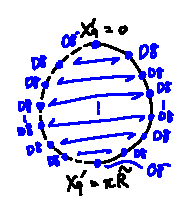
\includegraphics[width=100pt]{type1dual.eps}}
\caption{T-dual of Type I superstring theory.}
\label{type1dual.eps}
\end{figure}
Note that an O$9^-$-plane splits into two O$8^-$-plane.
Accordingly, tension and RR-charge reduce by $2$.


In the end, T-dual of Type I on $S^1$ is
\begin{align*}
 \textrm{Type IIA on } S^1/\ZZ_2 \quad \textrm{with} \quad  2 \textrm{ O$8^-$-plane }
 + 32 \textrm{ D$8$-branes }.
\end{align*}
Of course, one can consider further T-dualities along other directions.
Each T-duality doubles the number of O-planes, and hence,
reduces the tension and the RR-charges.
Namely, we have following relations:
\begin{align*}
 T_{\mathrm{O}p^\pm} = \pm 2^{p-4} \cdot T_{\mathrm{D}p} \quad (\textrm{tension}) \ , \quad
 Q_{\mathrm{O}p^\pm} = \pm 2^{p-4} \cdot Q_{\mathrm{D}p} \quad (\textrm{RR-charge}) \ .
\end{align*}

\section{Heterotic string theories}


We are ready to learn \textbf{Heterotic string theories} \cite{Gross:1984dd,Gross:1985fr,Gross:1985rr}. Heterotic string is a hybrid construction of the left-moving sector of the 26-dimensional bosonic string and the right-moving sector of 10-dimensional superstring. The 16 extra bosons of the left-movers are compactified on particular 16-dimensional tori, leading to $\SO(32)$ or $E_8\times E_8$. Since 16-dimensional tori have very special properties, we can also describe the left-movers in terms of 32 free fermions whose current algebra is associated to either  $\SO(32)$ or $E_8\times E_8$ with level $k=1$.  This hybridization of two different kinds of modes has been referred to as \textbf{heterosis}.


\subsection{Bosonic construction}

\subsubsection{Toroidal compactifications}
We have learnt the $S^1$ compactification so that we now generalize our analysis to the case of $D$-dimensions compactified on a torus $T^D$. The resulting theory is effectively $(26-D)$-dimensional. The torus is defined by identifying points in the D-dimensional internal space as follows (compact dimensions are labeled with capital letters):
\be \label {torusequiv}
	X^I \sim X^I + 2 \pi e^I_i n^i =X^I+2\pi W^I~, \qquad \textrm{for} \quad n^i \in \bZ~.
	\ee 
The $\mathbf{e}_i= \{e_i^I\}$  ($i= 1\cdots D$) are $D$ linear independent vectors called \textbf{vielbein} which generate a $D$-dimensional lattice $\Lambda$. In addition, the vielbein brings the metric into the standard Euclidean form:
\begin{align}	
	G_{ij} =\bfe_i\cdot\bfe_j= e^I_i e^J_j \delta_{IJ}, \qquad 	X^I \equiv e^I_i X^i\end{align}
The torus on which we compactify is obtained by dividing $\bR^D$ by $\Lambda$:
$$T^D = {{\bR}^D \over 2\pi \Lambda}~.$$
The momentum $p^I$ conjugate to the coordinates $X^I$ on the torus  
 is quantized as $\bfp \cdot \bfW \in\bZ$.	Therefore, the momentum $p$ takes its value on the dual lattice $\Lambda^*$ 
\[	\Lambda^* \equiv \{ e^{*Ii} m_i; \quad m_i \in \bZ \}, \qquad
		 G^{i j}=\bfe^{*i}\cdot\bfe^{*j}= e_I^{*i} e_J^{*j}\delta^{IJ}. \]

\begin{figure}[h]\centering
\includegraphics[width=10cm]{lattice}
\caption{Lattice and its dual lattice}
\end{figure}
The condition which a closed string in the compact directions has to satisfy is
$$
X ^I( \s+2\pi,\t)=X ^I( \s,\t)+2\pi W^I
$$
so that $W^I$ are analogues of winding number. We express the mode expansion for the compact direction as follows:
\begin{align}
X^I(z)&=x^I-i\sqrt{\ap\over2}p_R^I
\ln z+i\sqrt{\ap\over2}\sum_{m\neq0}{\alpha^I_m\over mz^m}, \nonumber\\
\overline X^I(\bz)&={\wt x}^I-i\sqrt{\ap\over2}{p^I_L}
\ln \bz+i\sqrt{\ap\over2}\sum_{m\neq0}{{\wt\alpha}^I_m\over m\bz^m}.\nonumber
\end{align}
where the zero modes are 
\begin{align}
\bfp_L := p^I_L &=\frac{1}{\sqrt{2}} \left[\sqrt{\a'}p^I + \frac {W^I}{\sqrt{\a'}}\right] =\frac{1}{\sqrt{2}}\left[ \sqrt{\ap}e^{* I i} m_i + \frac {e^I_i} {\sqrt{\ap}}  n^i\right]~,\cr
\bfp_R := p^I_R &=\frac{1}{\sqrt{2}} \left[\sqrt{\a'}p^I - \frac {W^I}{\sqrt{\a'}}\right] =\frac{1}{\sqrt{2}}\left[ \sqrt{\ap}e^{* I i} m_i - \frac{e^I_i} {\sqrt{\ap}}  n^i\right]~. 
\end{align}
The mass formula and the level matching condition are now
\begin{align}
\ap M^2&=2(N+\wt N-2) + (\ap p_Ip^I+\frac1{\ap} W_IW^I)\cr
&=2(N+\wt N-2) +(\ap m_im_jG^{ij}+\frac1{\ap} n^in^jG_{ij})\cr
N-\wt N&=p_I W^I=m_in^i
\end{align}
As we have seen before,  the expressions for $p_L$ and $p_R$ suggest \textbf{T-duality} between the 
winding number $W^I$ and the momentum $p^I$.  In fact, \textbf{T-duality} is equivalence between a pair of compactification lattices $\bfe_i$ and
$\bfe'_i$ that are related as $\sqrt{\ap'}\bfe'_i = \frac{\bfe^{*i}}{\sqrt{\ap'}}$.  These two
compactifications give the same spectrum since
their allowed values of the momenta are related as
\be \label {tdualp}
		\bfp_L \leftrightarrow \bfp_L';\qquad \bfp_R \leftrightarrow -\bfp_R'\ee 
by interchanging the labels $m_i$ and $n^i$. 


Now let us combine the zero modes into the $(D+D)$-dimensional vectors $\bfP=(\bfp_L,\bfp_R)$. 
This construction treats $\Lambda$ and $\Lambda^*$ on equal footing 
as 
$$ 
\bfP=\bfE^{* i} m_i + \bfE_j n^j,
$$
where 
$$
	\bfE_j = \frac1{\sqrt{\ap}}\left( \bfe_j,  - \bfe_j  \right)~, \quad
	\bfE^{* i} = \sqrt{\ap}\left(\bfe^{*i}, \bfe^{*i}  \right).
$$
Note that the length of the lattice is normalized by the string length $\sqrt{\ap}=\ell_s$.
Hence $\bfP$ takes value in a $(D+D)$-dimensional lattice $\G_{D,D}$ 
spanned by $\{\bfE^{* i}\}$ and $\{\bfE_j\}$  that satisfies the following properties:
\begin{itemize}\setlength{\parskip}{-0.1cm}
\item \textbf{Lorentzian} if the signature of the metric $G$ is $((+1)^D,(-1)^D)$,
\item \textbf{integral} if $v\cdot w \in \bZ$ for all $v,w\in \G_{D,D}$,
\item \textbf{even} if $\G_{D,D}$ is integral and $v^2$ is even for all $v\in\G_{D,D}$, 
\item \textbf{self-dual} if $\G_{D,D} =(\G_{D,D})^*$,
\item \textbf{unimodular} if $\textrm{Vol}(\G_{D,D}) =  | \det G| = 1$.
\end{itemize}
In fact, the metric of this lattice is defined by
$$
\bfP\cdot\bfP'=(\bfp_L\cdot\bfp_L-\bfp_R\cdot\bfp_R)=m_in'^{i}+m'_in^{i}
$$
so that it is Lorentzian. Because of ${\bf P\cdot P}\in2\bZ$, it is even. The self-dual property will be shown in Homework. The unimodular property $\textrm{Vol}(\G_{D,D})=\textrm{Vol}(\G_{D,D})=1$ immediately follows from  the self-dual property. 
The  lattice $\G_{D,D}$  in the torus compactification of the string is called \textbf{Narain lattice}. 

 
 The partition function of the bosonic string compactified on a torus $T^D$ is easy to write down:
\[	Z^{\textrm{bos}}_{\G_{D,D}} = \frac 1 {\t_2^{(24-D)/2}| {\eta (q)}|^{48}}
		\sum_{(\bfp_R, \bfp_L) \in \G_{D,D}} q^{\frac{1}{2} \bfp_R^2} 
								\bar q^{\frac{1}{2} \bfp_L^2}
\]
where $| {\eta (q)}|^{48}$ is the bosonic oscillator contribution and $\t_2^{(24-D)/2}$ comes from
the integral of non-compact momenta. 
This is easy to generalize to Type II string compactified on $T^D$
$$
Z^{\textrm{Type II}}_{\G_{D,D}} = \frac 1 {\t_2^{(8-D)/2}| {\eta (q)}|^{24}} \frac14\Big| -\vartheta_2^4(\tau) + \vartheta_3^4(\tau) - \vartheta_4^4(\tau)\Big|^2
		\sum_{(\bfp_R, \bfp_L) \in \G_{D,D}} q^{\frac{1}{2} \bfp_R^2} 
								\bar q^{\frac{1}{2} \bfp_L^2}								
$$
which vanishes by virtue of the Jacobi-Riemann identity.

\subsubsection{Heterotic strings}\label{sec:Heterotic-bosonic}

After our discussion of toroidal compactifications, we are now prepared to introduce the ten-dimensional Heterotic string. 
As mentioned in the beginning, Heterotic string is a combination of the left-moving sector of the 26-dimensional bosonic string combined with the right-moving sector of the 10-dimensional superstring. The left-moving bosonic string is compactified on a 16-dimensional torus so that the momenta of the additional chiral bosons $X^I(\bar z)$ takes value on 16-dimensional lattice  $\G_{16}$, \textit{i.e} $\bfp_L\in\G_{16}$.
Hence, the partition function of Heterotic string can be written as
\begin{equation}\label{het-pf}
	Z^{\textrm{het}}(\tau )  = \frac 1 {\t_2^{4}\eta (q)^{12}\eta (\bar q)^{24}} \Big( -\vartheta_2^4(\tau) + \vartheta_3^4(\tau) - \vartheta_4^4(\tau)\Big)
		\sum_{\bfp_L \in \G_{16}} 	\bar q^{\frac{1}{2} \bfp_L^2}
\end{equation}
Here $\eta (q)^{8}\eta (\bar q)^{24}$ is the bosonic oscillator contribution, the $\t_2^{4}$ factor arises from the zero modes of the uncompactified transverse coordinates and $\vartheta^4_i/\eta (q)^{4}$ comes from the world-sheet fermions. The most interesting part of this partition function is the lattice sum 
$$
P(\tau):=\sum_{\bfp_L \in \G_{16}} 	\bar q^{\frac{1}{2} \bfp_L^2}
$$
Since the partition function \eqref{het-pf} should be invariant under the modular transformation $\SL(2,\bZ)$, the modular transformation of $\eta$ and $\vartheta_i$ tell us that
$$
T:P(\t+1)=P(\t)~,\qquad S:P(-1/\t)=\t^8P(\t)~.
$$
The invariance under T-transformation clearly demands that $\bfp_L^2\in 2\bZ$ so that $\G_{16}$ must be \textbf{even}.
 For the $S$-transformation, we
make use of the Poisson resummation formula
\[	\sum_{\bfp\in\Lambda}e^{-\pi\a(\bfp+\bfx)^2+2\pi i \bfy\cdot (\bfp+\bfx)}=\frac{1}{\textrm{Vol}(\Lambda) \a^{\dim \Lambda /2}}\sum_{\bfq\in\Lambda^*}e^{-2\pi i \bfq\cdot \bfx-\frac{\pi}{\a}(\bfy+\bfq)^2}	\]
which amounts to
$$
P(-1/\t)=\frac{\t^8}{\textrm{Vol}(\Lambda)}\sum_{ \bfp_L\in(\G_{16})^*} 	\bar q^{\frac{1}{2} \bfp_L^2}~.
$$
This requires that the lattice $\G_{16}$ is \textbf{self-dual}, \textit{i.e.} $(\G_{16})^*=\G_{16}$ so that  $\textrm{Vol}(\Lambda)=1$.



It turns out that there are only two even self-dual Euclidean lattices in 16 dimensions
\begin{itemize}\setlength{\parskip}{-0.1cm}
\item the root lattice of $E_8\times E_8$
\item the weight lattice of $\Spin(32)/\bZ_2$ 
\end{itemize}
The metric $G_{ij}$ of the root lattice of $E_8$ is the Cartan matrix of $E_8$ \footnote{Unfortunately, we do not have time to talk about exceptional Lie algebra or a classification of semi-simple Lie algebras \cite{kirillov2008introduction}. In particular, if you want to get some intuition of weight and root lattices, see \cite[Fig 7.3, Fig 8.1, Fig 8.2]{kirillov2008introduction} for $A_2$. If you want to understand the structure $E_8$ related to string theory, we refer to \cite[\S 6]{GSW}.}:
\begin{equation}\nonumber
\left (
\begin{smallmatrix}
 2 & -1 &  0 &  0 &  0 &  0 &  0 & 0 \\
-1 &  2 & -1&  0 &  0 &  0 &  0 & 0 \\
 0 & -1 &  2 & -1 &  0 &  0 &  0 & 0 \\
 0 &  0 & -1 &  2 & -1 &  0 &  0 & 0 \\
 0 &  0 &  0 & -1 &  2 & -1 &  0 & -1 \\
 0 &  0 &  0 &  0 & -1 &  2 & -1 & 0 \\
 0 &  0 &  0 &  0 &  0 & -1 &  2 & 0 \\
 0 &  0 & 0 &  0 &  -1 &  0 &  0 & 2
\end{smallmatrix}\right ). 		\qquad\qquad	 \raisebox{-.5cm}{\includegraphics[width=5cm]{Dynkin_diagram_E8}}
\end{equation}


Let us investigate the on-shell spectrum of Heterotic string more carefully. 
As usual, there is the tachyonic vacuum of the bosonic string. At the massless level we have oscillator excitations $\wt \a_{-1}^\mu|0\rangle$, $\wt \a_{-1}^I|0\rangle$ in  left-moving sector. The former transform like space-time vectors whereas the internal oscillator excitations correspond to the left-moving part of the Abelian $\U(1)^{16}$ gauge boson. They build the \textbf{Cartan subalgebra} of $E_8 \times E_8$ or $\SO(32)$. Both the root lattice of $E_8\times E_8$ and the weight lattice of $\Spin(32)/\bZ_2$  contain 480 vectors of (length)$^2=2$ and generate the 496-dimensional non-Abelian gauge bosons of these groups. Remarkably, although Heterotic strings are closed strings, gauge fields show up thanks to the extra 16-dimensional tori! This can be also understood as novel \textbf{stringy effect} and gauge groups are restricted only to either $E_8 \times E_8$ or $\SO(32)$ in order for the theory to be consistent. Moreover, we have seen that $\SO(32)$ gauge group appears in Type I string theory. As we will see in the subsequent lecture, this is not coincident because Type I and Heterotic $\SO(32)$ are related by \textbf{S-duality}.



As a result, the massless spectra of Heterotic string are as follows

\vspace{.3cm}
\noindent $\bullet$ Gravitons, B-fields, dilaton in 10d
$$
\psi^\mu_{-\frac12}|0\rangle_{\textrm{NS}}\otimes\wt\a_{-1}^\nu|0\rangle
$$
$\bullet$  their supersymmetric partners, gravitino and dilatino
$$
|\mathbf{s}\rangle_{\textrm{R}}\otimes\wt\a_{-1}^\nu|0\rangle
$$
$\bullet$ 496 gauge bosons of  $E_8\times E_8$ or $\SO(32)$
$$
\psi^\mu_{-\frac12}|0\rangle_{\textrm{NS}}\otimes\wt\a_{-1}^I|0\rangle~,\qquad \psi^\mu_{-\frac12}|0\rangle_{\textrm{NS}}\otimes|\bfp_L^2=2\rangle
$$
$\bullet$  496 supersymmetric partners, gaugini
$$
|\mathbf{s}\rangle_{\textrm{R}}\otimes\wt\a_{-1}^I|0\rangle~,\qquad |\mathbf{s}\rangle_{\textrm{R}}\otimes|\bfp_L^2=2\rangle
$$
Indeed, Heterotic string theory is 10d $\cN=1$ supergravity coupled to 10d $\cN=1$  $E_8\times E_8$ or $\SO(32)$  super-Yang-Mills theory so that it has 16 real supersymmetric charges.


\subsection{Fermionic construction}

The 16 bosonic fields compactified on the self-dual lattice can be described by fermionic fields, which is called \textbf{fermionization}. Therefore, we will describe fermionic construction of Heterotic string theory next.

The world-sheet action of Heterotic string theory is given by
\begin{align}
 S^{\textrm{m}} &= \frac{1}{4\pi} \int d^2 z\ \Big( \frac{2}{\alpha'} \partial X^\mu  \overline\partial X_\mu+\psi^\mu\overline\partial\psi_\mu+\wt \lambda^A\partial\wt\lambda_A\Big)\cr
S^{\textrm{gh}}&=\frac{1}{2\pi}\int d^2z \ (b\overline \partial c+\bar b \partial \bar c+\beta\overline \partial \g)
\end{align}
where $\mu$ are 10-dimensional indices and the right-moving sector is supersymmetric. In order for the theory to be Weyl-anomaly free,  the central charge 
$$
c^{\textrm{tot}}=c^X+c^\psi+c^{bc}+c^{\beta\gamma}+c^{\lambda}=10+\frac52-26+\frac{11}{2}+c^{\lambda}=c^{\lambda}-8
$$
should vanish. Since each Majorana-Weyl anti-chiral fermion $\wt\lambda^A$ contributes $\frac14$ to the central charge, we need 32 left-moving fermions $\wt\lambda^A$ in the action.


It turns out that  there are two possible boundary conditions on the left-moving
fermions $\wt\lambda_A$ which give rise to fully consistent string theories. If we impose the same boundary condition to all, it leads to $\SO(32)$ gauge group. On the other hand, if we impose one boundary condition to a half and the other boundary condition to the other half, we obtain $E_8\times E_8$ gauge group. 

\subsubsection{Heterotic $\SO(32)$ (HO)}
For Heterotic $\SO(32)$, we impose the same boundary condition to all the left-moving fermions as
\begin{align}
\wt \lambda^A(t,\sigma+2\pi)=+\wt \lambda^A
  (t,\sigma) &\qquad\qquad\textrm{ R: periodic
on cylinder}\cr
\wt \lambda^A(t,\sigma+2\pi)=-\wt \lambda^A
  (t,\sigma) &\qquad\qquad\textrm{ NS:
anti-periodic on cylinder}
\end{align}
so that there is a global symmetry $\SO(32)$ that rotates  $\wt\lambda^A$ ($A=1,\ldots,32$). In order for the theory to be consistent, we have to impose GSO projection on the left-moving sector. In HO theory, we pick only states with odd fermionic number in NS sector and those with even fermionic number
$$
P_{\textrm{NS}}^{\textrm{HO}}:=\frac{1-(-1)^F}{2}
$$
whereas we keep only the states with even fermion number 
$$
P_{\textrm{R}}^{\textrm{HO}}:=\frac{1+(-1)^F}{2}~.
$$
In addition, we have to impose the level matching condition
\be\label{level-matching}
N-a=\wt  N-\wt a
\ee
where the normal ordering constants in the left-moving sector are
$$
{\wt a}_{\textrm{NS}}=\frac{8}{24}+\frac{32}{48}=1~,\qquad {\wt a}_{\textrm{R}}=\frac{8}{24}-\frac{32}{24}=-1~.
$$
Here the first term comes from the left-moving bosonic field $\overline X^i$ and the second term comes from $\wt \lambda^A$. Hence, the R sector contains only massive states. Contrary to the supersymmetric right-mover,  the Tachyon state $ |0\rangle_{\textrm{NS}}$ in the NS sector is preserved under the GSO projection. However, there is no corresponding state in the right-moving sector so that it does not obey the level matching condition \eqref{level-matching}.  As a result, the left-moving Tachyon is not included in the spectrum. Then, the first excited states after the GSO projection in the NS sector are
\begin{align}
\a^i_{-1} |0\rangle_{\textrm{NS}} \,&,\qquad (\mathbf{8_v},\mathbf{1}) \cr
\wt \lambda^A_{-1/2} \wt \lambda^B_{-1/2} |0\rangle_{\textrm{NS}}\,&, \qquad  (\mathbf{1},\textbf{adj}) \nonumber
\end{align}
where the bold letters are the representations of $\SO(8)\times \SO(32)$. The adjoint representation $\textbf{adj}$ of $\SO(32)$ is the antisymmetric tensor with dimension $32 \times 31/2 = \textbf{496}$. The following table shows the massless spectrum of HO where the first row represent the 10d $\cN=1$ supergravity multiplet whereas the second row shows  $\cN = 1$ gauge multiplet in the adjoint of $\SO(32)$ as we have seen in the bosonic construction.
\begin{table}[h] \centering
\begin{tabular}{ |c|c|c| } 
 \hline
Left$\backslash $Right & ${\bf 8_v}$ & ${\bf 8_c}$ \\ \hline
 $ (\mathbf{8_v},\mathbf{1})$ & ${\bf 1} \oplus {\bf 28}  \oplus {\bf 35}$ & ${\bf 8_s}\oplus{\bf 56_c}$ \\ 
  & $\phi \ \ B_{\mu\nu} \ \ G_{\mu\nu}$ & $\lambda^+ \ \ \psi^-_m$ \\ \hline
  $(\mathbf{1},\textbf{496})$ & $\SO(32)$ gauge boson &  $\SO(32)$ gaugini \\ 
    & $A^\mu_{[A,B]}$ & $\eta_{[A,B]}$ \\ 
 \hline
\end{tabular}
\end{table}

\subsubsection{Heterotic $E_8\times E_8$ (HE)}
The second Heterotic string theory is obtained by dividing the $\wt \lambda^A$ into two sets of 16 with independent boundary conditions,
$$
\wt\lambda^A(t,\sigma+2\pi)=\left\{ \begin{matrix}\e_1 \wt\lambda^A(t,\sigma) & \quad~ A=1,\ldots,16\\ \e_2 \wt\lambda^A(t,\sigma) & \qquad A=17,\ldots,32  \end{matrix}\right.
$$
where $\e_i=\pm1$. Therefore, in the left-moving sector,  we need to take the following boundary conditions into account 
$$
(\textrm{NS}_1,\textrm{NS}_2)~,\quad (\textrm{R}_1,\textrm{NS}_2)~,\quad (\textrm{NS}_1,\textrm{R}_2)~,\quad (\textrm{R}_1,\textrm{R}_2)~.
$$
Consequently, the global symmetry is broken to $\SO(16)_1\times\SO(16)_2$. The GSO projection is imposed to the two sets of left-movers independently:
$$
P_{\textrm{NS}_i}^{\textrm{HE}}:=\frac{1-(-1)^F}{2}
~\qquad
P_{\textrm{R}_i}^{\textrm{HE}}:=\frac{1+(-1)^F}{2}~.
$$
We also apply for the level-matching condition \eqref{level-matching}. The normal ordering constant in each boundary condition is
$$
{\wt a}_{\textrm{NS}_1,\textrm{NS}_2}=1~,\qquad {\wt a}_{\textrm{R}_1,\textrm{NS}_2}={\wt a}_{\textrm{NS}_1,\textrm{R}_2}=\frac{8}{24}+\frac{16}{48}-\frac{16}{24}=0~,\qquad {\wt a}_{\textrm{R}_1,\textrm{R}_2}=-1~.
$$
Again, $ (\textrm{R}_1,\textrm{R}_2)$ boundary condition has only massive states. Although the Tachyon state $ |0\rangle_{\textrm{NS}_1,\textrm{NS}_2}$ in the NS sector is preserved under the GSO projection, it does not obey the level-matching condition  \eqref{level-matching} so that it is not present in the spectrum. Then, the massless states are
\begin{align}
\a^i_{-1} |0\rangle_{\textrm{NS}_1,\textrm{NS}_2} \,&,\qquad (\mathbf{8_v},\mathbf{1}) \cr
\wt \lambda^A_{-1/2} \wt \lambda^B_{-1/2} |0\rangle_{\textrm{NS}_1,\textrm{NS}_2}\,&, \qquad  (\mathbf{1},\textbf{adj},\mathbf{1}) \ \textrm{or} \ (\mathbf{1},\mathbf{1},\textbf{adj})  \label{massless}
\end{align}
where the bold letters are the representations of $\SO(8)\times \SO(16)_1\times \SO(16)_2$. Note that the GSO projection requires either $1\le A,B\le16$ or $17\le A,B\le32$ in \eqref{massless}. The adjoint representation of $\SO(16)$ is of $16\times15/2=\textbf{120}$ dimension.

In $ (\textrm{R}_1,\textrm{NS}_2)$ and $(\textrm{NS}_1,\textrm{R}_2)$, the ground states are massless since the normal ordering constant is zero. Since the 16 $\wt \lambda_0^A$ zero modes form 8 raising and 8 lowering operators
$$
\wt \lambda_0^{K\pm} = 2^{-1/2}(\wt \lambda_0^{2K-1} \pm i\wt \lambda_0^{2K})~ , \qquad  K = 1,\ldots, 8 \ \textrm{or} \ K = 9,\ldots, 16~,
$$
the $2^{8}=\textbf{256}$-dimensional spinor representation of $\SO(16)$ becomes massless.
However, the GSO projection picks positive chirality $\textbf{128}$ out of $\textbf{256}=\textbf{128}+\textbf{128}'$ in the Ramond sector. Hence, the ground states are $(\mathbf{1},\textbf{128},\mathbf{1})$ and $(\mathbf{1},\mathbf{1},\textbf{128})$ under $\SO(8)\times \SO(16)_1\times \SO(16)_2$ in $ (\textrm{R}_1,\textrm{NS}_2)$ and $(\textrm{NS}_1,\textrm{R}_2)$, respectively .

All in all, the left-moving massless states form the representations of $\SO(8)\times \SO(16)_1\times \SO(16)_2$
$$
\bf (8_v,1,1) + (1,120,1) + (1,1,120) + (1,128,1) + (1,1,128)
$$
This spectrum strongly suggests that gauge symmetry is enhanced $\SO(16)\to E_8$ because $E_8$ has dimension $\bf 120+128=248$ which is also the dimension of the adjoint representation $E_8$. In fact, $E_8$ has an $\SO(16)$ subgroup under which the $E_8$ adjoint $\bf 248$ transforms as $\bf 120 + 128$. Hence, the massless spectrum is the  10d $\cN=1$ supergravity multiplet plus an  $\cN=1$ $E_8 \times E_8$ gauge multiplet. Even in fermionic construction, we have reproduce the 496-dimensional adjoint representations of both $\SO(32)$ and $E_8\times E_8$ gauge groups. 


\subsubsection{No D-branes in  Heterotic strings}
We have seen that D-branes are charged to RR fields in Type II theories. However, there is no RR field in Heterotic string theories because there is only world-sheet supersymmetry in the right-moving sector. In other words, although the RR $(p+1)$-form field strength $G$ in Type II theories can be expressed as
$$
G=\overline \psi^L \G^{\mu_1\cdots \mu_{p+1}}\psi^R~,
$$
there is no $\psi^L$ in Heterotic string theories. 
Hence, there is no D-brane in Heterotic string theories. Consequently, Heteroting string theories are the theories of closed strings\footnote{However Polchinski argues in \cite{Polchinski:2005bg} that there exist open Heterotic strings.}. However, apart from the fundamental strings, there are extended objects, \textbf{NS5-branes or Heterotic fivebranes}, in Heterotic string theories and they are magnetically charged under the $B$-field.




\section{Supergravity}

String theory includes massless states as well as massive states.
However, in a low-energy(IR) region, we do not see the stringy massive states 
because the mass $M^2 \sim \frac{1}{\alpha'} \sim \frac{1}{\ell_s^2}$ is assumed to be very heavy.
Therefore, in the IR limit, we can describe the theory by so called \textbf{effective theory}, 
which only contains the lightest particles(states).
The effective theory, of course, does not contain all the information of the original theory, 
however, it does give us some information of the original theory.


For the bosonic string theory the lightest particles are the massless states (except non-physical tachyon),
and we saw that the effective theory is (Lecture 4)
\begin{align*}
 S_\mathrm{eff} = \frac{1}{2\kappa_{26}^2} \int d^{26} X \sqrt{-G} e^{-2\Phi} \left[
 R -\frac{1}{12} H_{\mu\lambda\rho}H^{\mu\lambda\rho}
 +4 \nabla^\lambda\Phi \nabla_\lambda\Phi  \right] \ ,
\end{align*}
where $2\kappa_{26}^2$ is a gravitational coupling and it is related to
the Newton constant as $2\kappa_{26}^2 = 16 \pi G_N$.
What we will see below is supersymmetric versions of this,
that are effective theories of IIA/IIB superstring theory and
called type \textbf{IIA/IIB SUGRA} (SUpersymmetric GRAvity).


\subsection{Local SUSY}

Before going to the details of the IIA/IIB SUGRA
let us see general features of SUGRA.

First of all, in order to define spinors in a curved space
we need a vielbein $e_M^a(x^P)$, which transform a local coordinate $x^M$
into a tangent space coordinate (tangent vector) $x^a$ and vice versa (see also Fig.~\ref{tangent.eps}):
\begin{figure}[htb]
\centerline{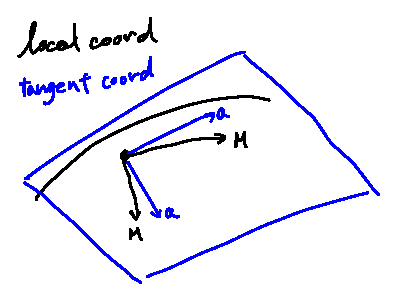
\includegraphics[width=200pt]{tangent.eps}}
\caption{Local coordinate and tangent coordinate.}
\label{tangent.eps}
\end{figure}
\begin{align*}
 x^a = e^a_M x^M \ , \quad x^M = e^M_a x^a \ ,
\end{align*}
which is defined through space-time metric $G_{MN}$ by
\begin{align*}
 G_{MN}(x^P) = \eta_{ab} e_M^a(x^P) e_N^b(x^P)  \ .
\end{align*}
Now we can use spinor representations and gamma matrices thanks to the vielbein:
\begin{align*}
 \{\Gamma^a,\Gamma^b\} = 2\eta^{ab} \ .
\end{align*}



In the case that a theory includes gravity
translation invariance is promoted to general coordinate transformation invariance (the symmetry is localized).
Similarly, global Lorentz symmetry is promoted to local Lorentz symmetry (this is done by the vielbein):
\begin{align*}
 \Lambda^a_{\ b} e_a^M(x^P) e_N^b(x^P) \equiv \Lambda^M_{\ N}(x^P) \ .
\end{align*}
Gravity is nothing but a gauge field for general coordinate transformation.
In general, gauge field has gauge degrees of freedom
\begin{align*}
 \delta A_M = D_M \lambda \ ,
\end{align*}
and for gravity it is
\begin{align*}
 \delta e_M^a = D_M \lambda^a \ ,
\end{align*}
where $\lambda^a$ is a vector gauge transformation parameter, and $D_M$ is a covariant derivative.


Since the translation is promoted to local one
supersymmetry, whose square is roughly translation, should also be promoted to
local supersymmetry.
Correspondingly, there must be a gauge field that transforms with a spinor gauge parameter $\xi^\alpha$ as follows.
\begin{align*}
 \delta \psi_M^\alpha = D_M \xi^\alpha \ ,
\end{align*}
where $\psi_M^\alpha$ is called Rarita-Schwinger field or \textbf{gravitino}.


SUGRA theory always includes the two gauge fields, $e^a_M$ and $\psi^\alpha_M$,
and their action is given by
\begin{align*}
 S = \frac{1}{2\kappa_D^2}\int d^D x\ e\ \left[ R -2i \psi_M \Gamma^{MNP} D_N \psi_P \right] \ ,
\end{align*}
where $e = \det e_M^a$, and we omitted the spinor index $\alpha$.
The SUSY transformations for the fields are
\begin{align*}
 \delta_\epsilon e^a_M = i\ol\epsilon \Gamma^a \psi_m \ , \qquad
 \delta_\epsilon \psi_M = D_M \epsilon \ .
\end{align*}



\subsection{11d SUGRA}

Supersymmetry puts a strong constraint on the dimension of the theory.
If we limit ourselves to consider fields up to spin-$2$,
then, it is known that the highest dimension is $11$.
This is roughly because the D.O.F of fermions grows exponentially: $2^{[D/2]}$,
on the other hand, that of bosons grows as a power of $D$: 
$\frac{(D-1)(D-2)}{2}-1$ (graviton).
Therefore, to balance fermions and bosons we cannot go arbitrary higher.


Although the existence of fermions is crucial,
what we need, to see the connections to string theories,
is the bosonic part.


Let us see the action of the 11d SUGRA.
\begin{align*}
 2\kappa_{11}^2 S_{11} = \int d^{11}x \sqrt{ -G} \left[R -\frac{1}{2} K_{(4)}^{2}\right]
 -\frac{1}{6}\int d^{11}x\ M_{(3)} \wedge K_{(4)} \wedge K_{(4)} \ ,
\end{align*}
where $K_4 = d M_3$ is a field strength of a rank 3 anti-symmetric tensor $M_3$,
and $K_{(4)}^{2} = K_{(4)} \wedge * K_{(4)}$.
The 11d SUGRA consists of three fields;
one is the graviton $G_{MN}$ (44 states), the other boson is 
rank 3 anti-symmetric tensor $M_{(3)}$ (84 states),
and the gravitino $\psi_M$ (128 states).
We can see that the numbers of fermions and bosons are balanced.
Note that there is only one parameter $\kappa_{11}$,
which can be written in terms of Planck length $\ell_p$: 
$\frac{1}{2\kappa_{11}^2} = \frac{2\pi}{(2\pi \ell_p)^9}$.


You may wonder why we looked into such a non-interesting theory
in a sense that what we want is $10$ dimension, rather than $11$ dimension.
One reason is that the interesting $10$d SUGRA can be derived by
dimensional reduction from the $11$ SUGRA.
Other reason, which is rather surprising, will be clear later.


\subsection{10d Type IIA SUGRA}


Let us first write down the action $S_\mathrm{A}$, which is a sum of following three terms.
\begin{align*}
 &S_\mathrm{A,NS} = \frac{1}{2\kappa_{10}^2} \int d^{10}x \sqrt{ -G} e^{-2\Phi} \left[
 R +4 \partial_\mu \Phi \partial^\mu \Phi -\frac{1}{2} H_{(3)}^{2} \right] \ ,  \\
 &S_\mathrm{A,R} = \frac{1}{2\kappa_{10}^2} \int d^{10}x \sqrt{ -G} \left[
 -\frac{1}{2} G_{(2)}^{2} -\frac{1}{2} \wt G_{(4)}^{2} \right] \ ,  \\
 &S_\mathrm{A,CS} = -\frac{1}{4\kappa_{10}^2} \int B_{(2)} \wedge G_{(4)} \wedge G_{(4)} \ ,
\end{align*}
where $H_{(3)} = dB_{(2)}$, $G_{(2)} = dC_{(1)}$, $\wt G_{(4)} = G_{(4)} -C_{(1)} \wedge H_{(3)}$, $G_{(4)} =dC_{(3)}$,
and $2\kappa_{10}^2 = (2\pi \ell_s)^8/2\pi$.

The IIA fields are coming from reduction of $11$d SUGRA fields
(the compactified direction is denoted as $\theta$):
\begin{align*}
 &G_{MN} \Rightarrow G_{\mu\nu} \ , \quad G_{\mu\theta} \Rightarrow C_1 \ , \quad
 G_{\theta\theta} \Rightarrow \Phi \ ,  \\
 &M_{\mu\nu\theta} \Rightarrow B_{\mu\nu} \ , \quad M_{\mu\nu\rho} \Rightarrow C_{(3)} \ .
\end{align*}

In order to see the concrete reduction let us substitute following expression:
\begin{align*}
 &ds_{11}^2 = G_{MN} dx^M dx^N = G_{\mu\nu} dx^\mu dx^\nu +l_p^2 e^{2\sigma} (d\theta+C_{(1)})^2 \ , \\
 &M_{(3)} = C_{(3)} +B_{(2)} \wedge d\theta \ , \quad K_{(4)} = \wt G_{(4)} +H_{(3)} \wedge (d\theta +C_{(1)}) \ ,
\end{align*}
into the action, and then, the action becomes
\begin{align}
 S_{11} &\Rightarrow \frac{2\pi \ell_p}{2\kappa_{11}^2}\int d^{10}x \sqrt{ -G} \left[
 e^\sigma R -\frac{1}{2} e^{3\sigma} G_{(2)}^{2} -\frac{1}{2} e^{-\sigma} H_{(3)}^{2}
 -\frac{1}{2} e^{\sigma} \wt G_{(4)}^{2}
 \right] \cr
 &\qquad-\frac{2\pi \ell_p}{4\kappa_{11}^2}\int d^{11}x\ B_{(2)} \wedge G_{(4)} \wedge G_{(4)} \ .
 \label{eq:1}
\end{align}
Furthermore, we rescale the metric $G_{\mu\nu} = e^{-\sigma} G_{s,\mu\nu}$:
\begin{align*}
 \Rightarrow \frac{2\pi \ell_p}{2\kappa_{11}^2}\int d^{10}x \sqrt{ -G_s} \left[
 e^{-3\sigma} \left(R +9\partial^\mu\sigma\partial_\mu\sigma
 -\frac{1}{2} H_{(3)}^{2} \right)
 -\frac{1}{2} G_{(2)}^{2} -\frac{1}{2} \wt G_{(4)}^{2}
 \right] +\cdots \ .
 % -\frac{2\pi \ell_p}{4\kappa_{11}^2}\int d^{11}x\ B_2 \wedge G_4 \wedge G_4 \ .
\end{align*}
Therefore, we can identify $3\sigma = 2\Phi$.


Let us define $R = \ell_p e^\sigma$, which is a radius of the compactified circle.
Then, we have following relation.
\begin{align*}
 e^{3\sigma} = e^{2\Phi} \quad\Rightarrow\quad \left(\frac{R}{\ell_p}\right)^3 = g_s^2 \ .
\end{align*}
Furthermore, we compare the coupling constant of 11d SUGRA with reduction (\ref{eq:1}) 
and IIA SUGRA:
\begin{align*}
 \frac{2\pi R}{2\kappa_{11}^2} = \frac{e^{-2\Phi}}{2\kappa_{10}^2} \quad\Rightarrow\quad
 \frac{2\pi(2\pi R)}{(2\pi \ell_p)^9} = \frac{2\pi}{g_s^2(2\pi \ell_p)^8}
 \quad\Rightarrow\quad \frac{R}{\ell_p^3} = \frac{1}{\ell_s^2} \ .
\end{align*}
Combining the two relation we have $R = g_s \ell_s$.


\subsection{10d Type IIB SUGRA}


Let us first write down the action $S_\mathrm{B}$, which is a sum of following three terms.
\begin{align*}
 &S_\mathrm{B,NS} = \frac{1}{2\kappa_{10}^2} \int d^{10}x \sqrt{ -G}  e^{-2\Phi} \left[
 R +4 \partial_\mu \Phi \partial^\mu \Phi -\frac{1}{2} H_{(3)}^{2} \right] \ ,  \\
 &S_\mathrm{B,R} = \frac{1}{2\kappa_{10}^2} \int d^{10}x \sqrt{ -G} \left[
 -\frac{1}{2} G_{(1)}^{2} -\frac{1}{2} \wt G_{(3)}^{2} -\frac{1}{4} \wt G_{(5)}^{2} \right] \ ,  \\
 &S_\mathrm{B,CS} = -\frac{1}{4\kappa_{10}^2} \int C_{(4)} \wedge H_{(3)} \wedge G_{(3)} \ ,
\end{align*}
where $H_{(3)} = dB_{(2)}$, $G_{(1)} = dC_{(0)}$, $G_{(3)} = dC_{(2)}$, $G_{(5)} = dC_{(4)}$, $\wt G_{(3)} = G_{(3)} -C_{(0)} H_{(3)}$, and $\wt G_{(5)} =G_{(5)} -\frac{1}{2}C_{(2)} \wedge H_{(3)} +\frac{1}{2} B_{(2)} \wedge G_{(3)}$.

As we saw in the string theory analysis the string spectrum includes
self-dual 4-form.
The self-dual condition, in the language here, is $* \wt G_{(5)} = \wt G_{(5)}$,
which is different from E.O.M $d*\wt G_{(5)} =0$ or Bianchi id $d \wt G_{(5)} = 0$.
Hence, the condition must be imposed by hand.
This is problematic when you quantize the theory,
however, it is not problem for our purpose.


% \subsection{Electro-magnetic duality}

% Since we have



\section{String dualities}


In the previous lectures we saw that there exist so called T-duality,
which relates IIA, IIB, and also Type I superstring theories.
Although it exchanges the space-time radius $R \leftrightarrow \wt R = \alpha'/R$
it does not affect coupling constant $g_s$.



Our argument is based on perturbation theory,
which means that the string coupling $g_s$ is small,
otherwise we cannot discuss ``1 string'' states.
Therefore, we do not know what happen in a strong coupling region $g_s \gg 1$.
Since the electro-magnetic duality inverse the coupling
we may wonder the same thing could happen in the string theory.



\subsection{S-duality of Type IIB SUGRA}

Let us write the action so that we can see the hidden symmetry of the action.
We use $G_{E,\mu\nu} = e^{-\Phi/2} G_{\mu\nu}$, $\tau = C_{(0)} +ie^{-\Phi}$,
\begin{align*}
 \mathbb M = \frac{1}{\Im \tau}
 \begin{pmatrix}
  |\tau|^2 & -\Re \tau \\ -\Re \tau & 1
 \end{pmatrix} \ , \qquad
 \mathbb F_{(3)} =
 \begin{pmatrix}
  H_{(3)} \\ G_{(3)}
 \end{pmatrix} \ ,
\end{align*}
and the action becomes
\begin{align*}
 S_\mathrm{B} = \frac{1}{2\kappa_{10}^2} \int d^{10}x \sqrt{ -G_E} \left[
 R_E - \frac{\partial_\mu \tau \partial^\mu \ol\tau}{2(\Im \tau)^2}
 -\frac{1}{2} \mathbb F_{(3)} \cdot \mathbb M \cdot \mathbb F_{(3)}
 -\frac{1}{4} \wt G_{(5)}^2
 \right]
 -\frac{1}{4\kappa_{10}^2} \int C_{(4)} \wedge \mathbb F_{(3)}^T \wedge \epsilon \mathbb F_{(3)} \ ,
\end{align*}
where $\epsilon = \begin{pmatrix} 0 & 1 \\ -1 & 0 \end{pmatrix}$.
This action is invariant under the $SL(2,\mathbb R)$ transformation:
\begin{align*}
 \tau' = \frac{a\tau +b}{c\tau +d} \ , \quad
 \mathbb M' = (\Lambda^{-1})^T \mathbb M \Lambda^{-1} \ , \quad
 \mathbb F_{(3)}' = \Lambda \mathbb F_{(3)} \ , \quad
 \Lambda =
 \begin{pmatrix}
  d & c \\ b & a
 \end{pmatrix} \ .
\end{align*}
$G_E$ and $C_{(4)}$ are invariant under the transformation.


Let us consider consider D-branes coupled to the RR-fields.
D$3$-brane is invariant because $C_{(4)}$ is invariant.
$5$-branes (NS$5$ and D$5$) are magnetically coupled to 2-form fields ($B_{(2)}$ and $C_{(2)}$),
therefore,
\begin{align*}
 \mathbb F_{(3)}' = \Lambda \mathbb F_{(3)} \quad\Rightarrow\quad
 d\mathbb F_{(3)}' =
 \begin{pmatrix}
  J_\mathrm{NS5}' \\ J_\mathrm{D5}'
 \end{pmatrix} =
 \Lambda 
 \begin{pmatrix}
  J_\mathrm{NS5} \\ J_\mathrm{D5}
 \end{pmatrix} \quad\Rightarrow\quad
 \begin{pmatrix}
  \mathrm{NS5}' \\ \mathrm{D5}'
 \end{pmatrix} = \Lambda
 \begin{pmatrix}
  \mathrm{NS5} \\ \mathrm{D5}
 \end{pmatrix} \ .
\end{align*}
Strings (F$1$ and D$1$) are electrically coupled to 2-form fields,
hence, have a following action
\begin{align*}
 S= \int_\mathrm{F1} B_{(2)} + \int_\mathrm{D1} C_{(2)} +\cdots \ .
\end{align*}
this should be invariant, therefore,
\begin{align*}
 \begin{pmatrix}
  \mathrm{F1} & \mathrm{D1}
 \end{pmatrix}
 \begin{pmatrix}
  B_{(2)} \\ C_{(2)}
 \end{pmatrix} \quad\Rightarrow\quad
 \begin{pmatrix}
  \mathrm{F1}' & \mathrm{D1}'
 \end{pmatrix} =
 \begin{pmatrix}
  \mathrm{F1} & \mathrm{D1}
 \end{pmatrix} \Lambda^{-1} \quad\Leftarrow\quad
  \begin{pmatrix}
  B_{(2)}' \\ C_{(2)}'
  \end{pmatrix} = \Lambda
  \begin{pmatrix}
  B_{(2)} \\ C_{(2)}
 \end{pmatrix} \ .
\end{align*}

Due to the Dirac quantization condition, the electric and the magnetic charges
must be integers, and hence, the true symmetry is $SL(2,\ZZ)$.

In the case of $\Lambda = S =
\begin{pmatrix}
 0 & 1 \\ -1 & 0
\end{pmatrix}$ fields transform
$\tau \leftrightarrow -1/\tau$, $\mathrm{F1} \leftrightarrow \mathrm{D1}$, and $\mathrm{NS5} \leftrightarrow \mathrm{D5}$.
Especially, if $\langle C_0 \rangle = 0$ $g_s \leftrightarrow 1/g_s$.
Therefore, this is a strong-weak duality !
and typically called \textbf{S-duality}.


Other elements of $SL(2,\ZZ)$ lead
infinitely many bound states of F$1$ and D$1$: $(p,q)$-string,
and those of NS$5$ and D$5$: $(p,q)$ 5-branes.


The argument here implies that IIB superstring theory has also $SL(2,\ZZ)$ symmetry,
and there many evidences for it but there is no proof so far.



\subsection{M-theory}


Since the IIB theory has $SL(2,\ZZ)$ symmetry,
we may expect the similar thing happens in IIA as well.
However, we immediately notice, e.g. that there is no partner for $B_{(2)}$ field, etc.



For IIA superstring theory, rather surprising phenomenon happens
in strong coupling region.
As we saw in the dimensional reduction of 11d SUGRA
we have $R = g_s \ell_s$.
This means that when we consider strong coupling region another space-time direction
emerges (de-compactification) !!
So far, this deduction is purely from SUGRA analysis, however,
if we assume that the 11d SUGRA is an effective theory of something like ``string''
theory, then, further miraculous coincidence happens.

Witten proposed such a ``string''-like theory and put a name, \textbf{M-theory}.
According to him the M stands for Magic, Mysterious, or Membrane.
Some people also include Matrix, etc. so why not come up with your own M !


Since the 11d SUGRA has 3-form anti-symmetric fields
there must be corresponding objects that coupled to the field electrically and magnetically.
They are called \textbf{M2-brane} and \textbf{M5-brane},
which are $(1+2)$- and $(1+5)$-dimensional objects, respectively.
Let us assume that they have following tensions and charges
\begin{align*}
 T_{M2} = \mu_{M2} = \frac{2\pi}{(2\pi \ell_p)^3} \ , \qquad
 T_{M5} = \mu_{M5} = \frac{2\pi}{(2\pi \ell_p)^6} \ .
\end{align*}

When we put this M-theory on a circle $S^1$, then, it should reduce to
the IIA superstring theory.
Let us see this by comparing the branes and their tensions (see Table~\ref{table:001}).
\begin{table}[htbp]
 \begin{center}
  \caption{Wrapped or unwrapped M-branes and corresponding string and D-branes,
  with their tensions.}
  \vspace{4pt}
  \label{table:001}
\begin{tabular}{c|cccccc}
 Dimension & $0$ & $1$ & $2$ & $4$ & $5$ & $6$ \\
 \hline
 M on $S^1$ & KK-mom. & M2/$S^1$ & M2 & M5/$S^1$ & M5 & KK-mono. \\
 & $\frac{1}{R}$ & $\frac{2\pi\cdot2\pi R}{(2\pi \ell_p)^3}$ & $\frac{2\pi}{(2\pi \ell_p)^3}$ & $\frac{2\pi\cdot2\pi R}{(2\pi \ell_p)^6}$ & $\frac{2\pi}{(2\pi \ell_p)^6}$ & $\frac{2\pi(2\pi R)^2}{(2\pi \ell_p)^9}$ \\
 \hline
 IIA & D$0$ & F$1$ & D$2$ & D$4$ & NS$5$ & D$6$ \\
 & $\frac{2\pi}{g_s (2\pi \ell_s)}$ & $\frac{2\pi}{(2\pi \ell_s)^2}$ & $\frac{2\pi}{g_s (2\pi \ell_s)^3}$ & $\frac{2\pi}{g_s (2\pi \ell_s)^5}$ & $\frac{2\pi}{g_s^2 (2\pi \ell_s)^6}$ & $\frac{2\pi}{g_s (2\pi \ell_s)^7}$ \\
\end{tabular}
\end{center}
\end{table}
You should confirm that the tensions perfectly agree.


Note that M-theory is NOT even defined in a sense that we do not know how to quantize
the M-branes.
However, the existence of such a theory tells us a lot.
Especially, even though no effective theory of M$5$-branes in flat space is known,
M$5$-branes wrapped on Riemann manifolds leads amazing relation between
a $d$-dim topological theory and $6-d$ supersymmetric gauge theories
(typical one is M$5$ wrapped on Riemann surface and the relation is called AGT),
which is an ongoing, hot research topic.

%
%\subsection{D-brane dynamics}
%
%There is so called Dirac-Born-Infeld action, which is an effective action
%for D-branes.
%It describes motion of the D-branes as well as gauge field living on their world-volume.
%
%Let us consider a simple set up (see Fig.~\ref{D1D2.eps}).
%\begin{figure}[htb]
%\centerline{\includegraphics[width=250pt]{D1D2.eps}}
%\caption{D$1$-brane and its T-dual D$2$-brane.}
%\label{D1D2.eps}
%\end{figure}
%The space-time is $\RR_t \times \RR \times S^1$
%and the metric is $ds^2 = \eta_{\mu\nu} dx^\mu dx^\nu$.
%D$1$-brane locates at $X_2$ ($\sim X_2 +2\pi R$),
%and D$2$-brane has Wilson line $A_2$ ($\sim A_2 +\frac{1}{\wt R}$).
%Note that here $A_2$ is not a 2-form but $A_{\mu=2}$.
%T-duality relates these quantities (Lecture 9):
%\begin{align*}
% X_2 = 2\pi \alpha' A_2 \ .
%\end{align*}
%Now consider vibrating D$1$-brane $X^2 = X^2(x^1)$ (see Fig.~\ref{vibD1.eps}).
%\begin{figure}[htb]
%\centerline{\includegraphics[width=120pt]{vibD1.eps}}
%\caption{Vibrating D$1$-brane.}
%\label{vibD1.eps}
%\end{figure}
%It maps to a field strength $F_{12} = \partial_1 X_2(x^1) \neq 0$ on D2-brane.
%Suppose the vibrating D$1$-brane is described by Nambu-Goto action
%\begin{align*}
% S_\textrm{D1} &= -T_\textrm{D1} \int d^2x \sqrt{-\det \left( G_{\mu\nu} \frac{\partial X^\mu}{\partial x^a} \frac{\partial X^\nu}{\partial x^b} \right)} \quad\textrm{with}\quad
% X^0 = x^0 \ , \quad X^1 = x^1 \ , \cr
% &= -T_\textrm{D1} \int dx^0 dx^1 \sqrt{1 +\left(\frac{\partial X^2}{\partial x^1} \right)^2} \ .
%\end{align*}
%This expression seems to coincide with
%\begin{align*}
% S_\textrm{D2} &= -T_\textrm{D2} \int d^3x \sqrt{-\det \left( G_{\mu\nu} \frac{\partial X^\mu}{\partial x^a} \frac{\partial X^\nu}{\partial x^b} +2\pi \alpha' F_{ab} \right)}  \cr
% &= -T_\textrm{D2} \cdot 2\pi \wt R\cdot \int dx^0 dx^1 \sqrt{1 +\left(2\pi\alpha'F_{12} \right)^2} \ .
%\end{align*}
%
%
%From the dimension analysis D-brane tension should be the following form.
%\begin{align*}
% T_{\mathrm Dp} \sim \frac{\mathrm{mass}}{p\textrm{-dim vol}} \quad\Rightarrow\quad
% T_{\mathrm Dp} \sim \frac{1}{\ell_s^{p+1}} \ .
%\end{align*}
%From the argument above in order for the two action to coincide
%we need $T_\textrm{D1} = 2\pi \wt R T_\textrm{D2}$.
%On the other hand, we do not want $T_{\textrm{D}p}$ to depend on $R$ because
%$T_{\textrm{D}p}$ should be independent of space-time geometry.
%Note that D-brane effective theory is supposed to reproduce open string amplitude,
%whose leading contribution is the disk amplitude $\sim e^{-\langle \Phi \rangle}$.
%Thus, we propose
%\begin{align*}
% S_{\textrm{D}p} &= -T_{\textrm{D}p} \int d^{p+1}x e^{-\Phi(X)} \sqrt{-\det \left( G_{\mu\nu}
% \partial_a X^\mu \partial_b X^\nu +2\pi \alpha' F_{ab} \right)} \ .
%\end{align*}
%Then, the ration of effective tension is
%\begin{align*}
% \frac{T_{\textrm{D}1}^\mathrm{eff}}{T_{\textrm{D}2}^\mathrm{eff}}
% = \frac{T_{\textrm{D}1} e^{-\Phi}}{T_{\textrm{D}2} e^{-\wt\Phi}}
% =  \frac{T_{\textrm{D}1}}{T_{\textrm{D}2}} \cdot \frac{\wt R}{\ell_s} = 2\pi \wt R
% \quad\Rightarrow\quad T_{\textrm{D}1} = 2\pi \ell_s \cdot T_{\textrm{D}2} \ .
%\end{align*}
%Note that the dilation field transforms under T-duality as $e^{-\wt\Phi} = e^{-\Phi} \frac{\wt R}{\ell_s}$.
%For D-branes in superstring theory the correct normalization is
%$T_{\textrm{D}p} = \frac{2\pi}{(2\pi \ell_s)^{p+1}}$.
%
%
%
%We heavily used the fact that D$p$-branes couples to $C_{p+1}$.
%Let us consider a concrete coupling.
%It should be the following form.
%\begin{align*}
% S_{\textrm{D}p} = \cdots + \mu_{\textrm{D}p} \cdot \int d^{p+1}x e^{-\Phi}
% C_{\mu_1\cdots\mu_{p+1}}(X) \frac{\partial X^{\mu_1}}{\partial x^1 } \cdots
% \frac{\partial X^{\mu_{p+1}}}{\partial x^{p+1} }
% = \cdots +\mu_{\textrm{D}p} \cdot \int_{\textrm{D}p} e^{-\Phi} C_{(p+1)} \ .
%\end{align*}
%By considering T-duality we can conclude that
%$\mu_{\textrm{D}p} = \frac{2\pi}{(2\pi \ell_s)^{p+1}} = T_{\textrm{D}p}$ (up to a constant).
%Note that we have to use proper normalization of the RR-fields,
%depending on the context, which either string analysis or SUGRA analysis.
%The convention above is for string analysis.
%For SUGRA analysis it is (called canonically normalized one)
%\begin{align*}
% S_{\textrm{D}p} =
% \cdots +\mu_{\textrm{D}p} \cdot \int_{\textrm{D}p} C_{(p+1)} \ .
%\end{align*}
%
%
%
%
%Let us again vibrating D$1$-brane with the RR-coupling.
%T-duality connects the following two expression.
%\begin{align*}
% &S_{\textrm{D}1} =
% \cdots +\mu_{\textrm{D}1} \cdot \int dx^0 dx^1 e^{-\Phi}
% \left( C_{01} +C_{02} \frac{\partial X^2}{x^1}\right) \ , \\
% &S_{\textrm{D}2} =
% \cdots +\mu_{\textrm{D}2} \cdot \int dx^0 dx^1 dx^2 e^{-\wt \Phi}
% \left( \wt C_{012} +\wt C_{0} \cdot s\pi\alpha' F_{12} \right) \ ,
%\end{align*}
%where $C_{01} \leftrightarrow \wt C_{012}$, $C_{02} \leftrightarrow \wt C_{0}$, and $X^2 \leftrightarrow 2\pi\alpha' A_2$.
%This can be understood as follows (see Fig.).
%\begin{figure}[htb]
%\centerline{\includegraphics[width=250pt]{D0D2.eps}}
%\caption{D$0$-D$0$ bound state.}
%\label{D0D2.eps}
%\end{figure}
%The vibrating D$1$-brane consists of straight D$1$-brane along $x^1$
%and local vibration along $x^2$.
%After T-duality along $x^2$ the vibration part becomes D$0$-brane and gives
%$F_{12}\neq 0$.
%Generalization of the RR-coupling is
%\begin{align*}
% S_{\textrm{D}p} =
% \cdots +\mu_{\textrm{D}p} \cdot \int C_{RR} \wedge \exp(2\pi\alpha' F_{(2)}) \ ,
%\end{align*}
%where $C_{RR} = \sum_{n} C_{(n)}$.
%
%
%Finally, full general form of D$p$-brane action is given as follows.
%\begin{align*}
% S_{\textrm{D}p} &= -T_{\textrm{D}p} \int d^{p+1}x e^{-\Phi(X)} \sqrt{-\det \left( G_{ab}
% +2\pi \alpha' F_{ab} -B_{ab} \right)} \cr
% &\qquad +\mu_{\textrm{D}p} \cdot \int C_{RR} \wedge \exp(2\pi\alpha' F_{(2)}-B_{(2)}) \ ,
%\end{align*}
%where $G_{ab} = G_{\mu\nu} \partial_a X^\mu \partial_b X^\nu$ and
%$B_{ab} = B_{\mu\nu} \partial_a X^\mu \partial_b X^\nu$.
%
%
%\vspace{12pt}
%\noindent
%\textbf{Dirac quantization condition}


% Let us consider D$p$-brane located at $\bm x_{\perp} = (x_{p+1},\ldots,x_9) = \bm 0$.
% Then, the RR-coupling becomes
% \begin{align*}
%  \mu_{\textrm{D}p} \cdot \int_{\bm x_{\perp} = \bm 0} C_{p+1}
%  = \mu_{\textrm{D}p} \cdot \int_{\bm x_{\perp} = \bm 0} C_{p+1} \wedge \delta(\bm x_{\perp})
%  dx^{p+1} \cdots dx^9 \ .
% \end{align*}
% With the kinetic term the action is
% \begin{align*}
%  S = -\frac{1}{4\kappa_{10}^2} \int F_{(p+2)} \wedge * F_{(p+2)}
%  +\mu_{\textrm{D}p} \int C_{p+1} \wedge \delta(\bm x_{\perp})
%  dx^{p+1} \cdots dx^9 \ ,
% \end{align*}
% and the E.O.M is
% \begin{align*}
%  d*F_{(p+2)} = 2\kappa_{10}^2 \mu_{\textrm{D}p} \delta(\bm x_{\perp})
%  dx^{p+1} \cdots dx^9 \ .
% \end{align*}
% Integration over ball that perpendicular to the world-line of the D$p$-brane leads
% \begin{align*}
%  2\kappa_{10}^2 \mu_{\textrm{D}p} = 
% \end{align*}

%
%Let us consider a $(p+1)$-form RR field.
%The electrically coupled object is D$p$-brane and the magnetic one is D$(6-p)$-brane.
%The magnetic charge of the D$(6-p)$-brane is
%\begin{align*}
% \mu_{6-p} = \frac{1}{2\kappa_{10}^2} \int_{B^{p+3}} d F_{(p+2)} =
% \frac{1}{2\kappa_{10}^2} \int_{\partial B^{p+3}} F_{(p+2)} \ .
%\end{align*}
%Now consider D$p$-brane moving around D$(6-p)$-brane.
%\begin{align*}
% S \sim \mu_{p} \int_M C_{(p+1)} = \mu_{p} \int_{\partial^{-1}M} F_{(p+2)} \ ,
%\end{align*}
%where $\partial^{-1}M$ is manifolds whose boundary is $M$.
%The choice of $\partial^{-1}M$ is arbitrary, and does not affect the result.
%Consider $\partial^{-1}M_N -\partial^{-1}M_S$ surround the D$(6-p)$-brane.
%\begin{align*}
% \mu_{p} \int_{\partial^{-1}M_N} F_{(p+2)} -\mu_{p} \int_{\partial^{-1}M_S} F_{(p+2)}
% = \mu_{p} \mu_{6-p} 2\kappa_{10}^2 \in 2\pi \ZZ \ .
%\end{align*}
%The values $\mu_{p} = \frac{2\pi}{(2\pi \ell_s)^{p+1}}$,
%$2\kappa_{10}^2 = \frac{(2\pi \ell_s)^{8}}{2\pi}$ satisfy the quantization condition.
%
%
%
%Assume the condition works also for F$1$-string and NS$5$-brane,
%\begin{align*}
% T_\mathrm{F1} \cdot T_\mathrm{NS5} \cdot 2\kappa_{10}^2 g_s^2 = 2\pi \ ,
%\end{align*}
%where we are in the string frame.
%Since $T_\mathrm{F1} = \frac{2\pi}{(2\pi \ell_s)^2}$,
%\begin{align*}
% T_\mathrm{NS5} = \frac{2\pi}{T_\mathrm{F1} \cdot 2\kappa_{10}^2 g_s^2}
% = \frac{2\pi}{(2\pi \ell_s)^6 g_s^2} \ .
%\end{align*}


\section{Lecture 13}
\SN{Merge sections}

We will continue to learn string dualities extensively studied in the second string revolution after the seminal paper \cite{Witten:1995ex}. So far, we have learned

\vspace{.3cm}
\noindent $\bullet$ Type IIA and IIB are T-dual to each other

\vspace{.3cm}
\noindent $\bullet$ Type I is the orientifold projection of Type IIB 

\vspace{.3cm}
\noindent $\bullet$  Type IIB has $\SL(2,\bZ)$ symmetry so that it is self-dual under S-duality  

\vspace{.3cm}
\noindent $\bullet$  The strong coupling regime of Type IIA is described by M-theory on $S^1$

\vspace{.3cm}
\noindent In this lecture, we will learn

\vspace{.3cm}
\noindent $\bullet$  Heterotic $\SO(32)$ and $E_8\times E_8$ are T-dual to each other

\vspace{.3cm}
\noindent $\bullet$  Heterotic $\SO(32)$ is S-dual to Type I 

\vspace{.3cm}
\noindent $\bullet$ The strong coupling regime of  Heterotic $E_8\times E_8$ is described by M-theory on $S^1/\bZ_2$

\vspace{.3cm}
\noindent $\bullet$  Heterotic string on $T^4$ is dual to Type IIA on K3

\begin{figure}[h]\centering
\includegraphics[width=\textwidth]{duality-web}
\end{figure}

Even for these dualities, we can cover only key points in this lecture. More details can be found in  \cite{Polchinski,BBS}. Moreover, we  just see a tip of iceberg, and there are much more string dualities. Thus, 
I refer to good reviews  \cite{Aspinwall:1996mn,Forste:1996yd,Ooguri:1996ik,Polchinski:1996nb,Polchinski:1996na,Townsend:1996xj,Schwarz:1996bh,Sen:1996yy,Dijkgraaf:1997ip,Vafa:1997pm,Sen:1998kr} written during the second string revolution for this rich subject. All in all, these dualities tells us that quantum strings somehow see geometry from drastically different viewpoints. I hope you will get some feeling of it in this lecture.

\subsection{Heterotic T-duality} \label{sec:HeteroticT}

Let us consider the T-duality in Heterotic strings on a circle $S^1$ in \cite{Narain:1985jj,Narain:1986am,Ginsparg:1986bx}. In the bosonic construction, the bosonic left-moving sector is compactified on an even self-dual Euclidean lattice of 16-dimensions. There are only two such lattices: the weight lattice $\G_{\SO(32)}$ of $\SO(32)$ and the root lattice $\G_{E_8}\oplus \G_{E_8}$ of $E_8\times E_8$ as we have seen in \S\ref{sec:Heterotic-bosonic}.


One may also describe the compactification on a circle $S^1$ in terms of lattices. As we have seen, the left-moving and right-moving momenta compactified boson takes the value on  the lattice $\Gamma^{1,1}$ of the Lorentzian signature. Hence, the circle compactification results in adding ($\oplus$) the lattice $\Gamma^{1,1}$ to the original lattice. 



It is a useful mathematical fact that for Lorentzian
lattices, there is 
only unique even unimodular Lorentzian lattice for each rank. Therefore, the theorem implies 
$$\G_{\SO(32)}\oplus \Gamma^{1,1} \cong\G^{1,17}
\cong  \G_{E_8}\oplus \G_{E_8}\oplus \Gamma^{1,1}~.$$
Together with the metric $G$ and the $B$-field, 
they parameterize the
moduli space 
\begin{equation}\label{eq:Mhettoroidal}
{\cal M}=\left. \frac{\mathrm{O}(1,17)}{\mathrm{O}(1)\times \mathrm{O}(17)}\right/ \mathrm{O}(1,17; \bZ) ,
\end{equation}
where $\mathrm{O}(1,17; \bZ)$ is the T-duality group. It is called \textbf{Narain moduli space}.
Different points in the moduli space correspond to physically distinct compactifications, e.g. the gauge groups can be different, although always of rank 18. At generic points it is $\U(1)^{18}$ that corresponds to the fact that Wilson loops generically breaks 10d gauge group to $\U(1)^{18}$.



However, there are special subspaces of the moduli space where it is enhanced.
This moduli space has exactly two asymptotic boundary points, one associated to the
decomposition $\G^{1,17}\cong \G_{E_8}\oplus \G_{E_8}\oplus\G^{1,1}$,
and the other to the decomposition $\G^{1,17}
\cong \G_{\SO(32)}\oplus\G^{1,1}$.  
We assign the boundary points the 
interpretations of types HE and HO strings, or large radius and small radius.
T-duality will relate these interpretations.  



In fact, starting from either Heterotic theory, there is a simple choice of
Wilson line which breaks the gauge group to 
$\SO(16)\times \SO(16) \times \U(1)\times  \U(1)$.   If we leave this
group unbroken, then the only remaining parameter is the radius. An analysis of the massive states shows
that if we map $R\to 1/R$ while exchanging KK momenta
and winding modes, then the two Heterotic theories are exchanged \cite[\S11.6]{Polchinski}.



More generally, upon a compactification of Heterotic strings  on a $D$-dimensional torus $T^D$, momenta take the values on  an even self-dual Lorentzian lattice $\G^{D,D+16}$. Therefore, the Narain moduli space becomes
\be\label{Narain}
{\cal M}=\left. \frac{\mathrm{O}(D,D+16)}{\mathrm{O}(D)\times \mathrm{O}(D+16)}\right/ \mathrm{O}\left(D,D+16; \bZ\right)~.
\ee
which is  $D(D+16)$-dimensional.





\subsection{S--duality between Type I and Heterotic $\SO(32)$}


Now let us see S-duality between Type I theory  and Heterotic  $\SO(32)$ theory  \cite{Witten:1995ex,Dabholkar:1995ep,Hull:1995nu,Polchinski:1995df} from low-energy effective actions.



One can obtain Type I supergravity action from Type IIB by setting to zero the IIB fields $C_0$, $B_2$, and $C_4$ that are removed by the $\O$ projection. In addition, we include $\SO(32)$ gauge fields with appropriate dilaton dependence 
\begin{align}\label{TypeI}
S_{\textrm{I}}&=S_{\textrm{grav}}+S_{\textrm{YM}}\cr
S_{\textrm{grav}}&= \frac{1}{2\kappa_{10}^2} \int d^{10}x \sqrt{ -G}   \,\left[
e^{-2\Phi}( R +4 \partial_\mu \Phi \partial^\mu \Phi )-\frac{1}{2}| \wt G_{3}|^{2} \right] \cr
S_{\textrm{YM}}&=- \frac{1}{2g_{10}^2} \int d^{10}x \sqrt{ -G}\,  e^{-\Phi} \Tr_{V} |F_2|^2
\end{align}
where $F_2$ is the $\SO(32)$ field strength and the trace is in the vector representation. Here $G_3$ is the field strength of the RR 2-form $C_2$
$$
\wt G_{3}=dC_2-\frac{\kappa_{10}^2}{g_{10}^2}\omega_3
$$
with  the Chern-Simons 3-form
$$
\omega_3=\Tr_{V}\Big(AdA-\frac{2i}3 A^3\Big)~.
$$
The gauge coupling constant $g_{10}$ and the gravitational constant $\kappa_{10}$ are related by $\kappa_{10}^2/g_{10}^2 = \a'/4$, which is determined by anomaly cancelation. Under the gauge transformation $\delta A=d\lambda-i[A,\lambda]$, the Chern-Simons term transforms as
$$
\delta \omega_3=d \Tr_V(\lambda A)
$$
Hence, it comes with 
$$
\d C_2 = \frac{\kappa_{10}^2}{g_{10}^2} \Tr_V(\lambda dA)~.
$$

Heterotic strings have the same supersymmetry as Type I string and so we expect the same action. However, in the absence of open strings or RR fields the dilaton dependence should be $e^{-2\Phi}$ throughout:
\begin{align}\label{Het}
S_{\textrm{Het}}&=S_{\textrm{grav}}+S_{\textrm{YM}}\cr
S_{\textrm{grav}}&= \frac{1}{2\kappa_{10}^2} \int d^{10}x \sqrt{ -G}   \,e^{-2\Phi}\left[
 R +4 \partial_\mu \Phi \partial^\mu \Phi -\frac{1}{2}| \wt H_{3}|^{2} \right] \cr
S_{\textrm{YM}}&=- \frac{1}{2g_{10}^2} \int d^{10}x \sqrt{ -G}\,  e^{-2\Phi} \Tr_{V} |F_2|^2
\end{align}
where the 3-form $\wt H_3$ is the field strength of the $B$-field equipped with Chern-Simons form
$$
\wt H_{3}=dB_2-\frac{\kappa_{10}^2}{g_{10}^2}\omega_3~.
$$

Indeed the low-energy effective actions of Type I \eqref{TypeI} and Heterotic $\SO(32)$ \eqref{Het} are related by the following the field definitions (Homework)
\begin{align}
G_{\m\n}^{I} = e^{-\Phi^{H}} G_{\m\n}^{H} ~,&\qquad  \Phi^I = -\Phi^{H} \cr
\wt G_{3}^I = \wt  H_{3}^{H}~ ,&\qquad  A^I = A^{H} ~.
\end{align}
 Recalling that the vacuum expectation value of the dilaton is the string coupling $g_{st}=e^{\Phi}$, we see that the strong coupling limit of one theory is related to the weak coupling limit of the other theory and vice versa.

In Type I theory there are D1-branes and 
D5-branes that are electrically and magnetically charged under $C_2$, respectively. In Heterotic $\SO(32)$ theory, there are fundamental strings and NS5-branes that are electrically and magnetically charged under $B_2$, respectively. The S-duality 
maps them as \cite{Polchinski:1995df}
\begin{table}[h]\centering
\begin{tabular}{ccc}
Type I&$\leftrightarrow$& Heterotic SO(32)\\ \hline
D1-branes&$\leftrightarrow$&F-strings\\
D5-branes&$\leftrightarrow$&NS5-branes
\end{tabular}\end{table}

One can provide another evidence of this duality by looking at massless spectrum. We have seen that Heterotic $\SO(32)$ has massless fields:
\begin{enumerate}\setlength{\parskip}{-0.1cm}
\item $\bf 8_v$ of SO(8): bosonic right-moving  $X^i(z)$  
\item $\bf 8_c$ of SO(8):   fermionic right-moving $\psi^i(z)$
\item $\bf 32$ of SO(32):   left-moving Majorana-Weyl fermion $\wt\lambda^a(\bar z)$ 
\end{enumerate}
Correspondingly, one can see the massless BPS excitations from D1-strings stretched in the $x_1$-direction in Type I theory (Homework):
\begin{enumerate}\setlength{\parskip}{-0.1cm}
\item $\bf 8_v$ of SO(8): normal bosonic excitations of D1-D1 strings  
\item $\bf 8_c$ of SO(8):  right-moving fermionic  excitations of D1-D1 strings 
\item $\bf 32$ of SO(32):   left-moving fermionic  excitations of D1-D9 strings
\end{enumerate}

Further evidence of
this duality has been assembled by comparing tensions, $F_2^4$ interactions, so on \cite[\S14.3]{Polchinski}.	


\subsection{Heterotic $E_8\times E_8$ string from M-theory}

Now we shall consider the strong-coupling behavior of Heterotic $E_8\times E_8$ theory. Taking T-duality and S-duality, Heterotic $E_8\times E_8$ theory is dual to Type I theory. The T-dual to Type I theory is Type IIA theory on a line segment $S^1/\bZ_2$ where O8${}^-$-plane sit at the two ends and 16+16 D8 branes are distributed on  $S^1/\bZ_2$ as described in \S\ref{sec:TypeI'}. We call this theory \textbf{Type I' theory}. In the strong coupling regime, the 11th circle will emerge and it is described M-theory on $S^1\times S^1/\bZ_2$. 


\begin{figure}[h]\centering
\includegraphics[width=15cm]{HE-duality}
\caption{Duality web for Heterotic M-theory}
\end{figure}


Interestingly enough, the relative position of O8${}^-$-planes and D8-branes in Type I' string theory may be adjusted. This freedom goes away in the M-theory limit; the D8-branes have to be stuck at the O8${}^-$-planes, and they become the domain walls of M-theory, which are called \textbf{Ho\v{r}ava-Witten domain wall} or \textbf{M9-branes} \cite{Horava:1995qa,Horava:1996ma}. 


Its low-energy effective description is given by 11d supergravity on $S^1/\bZ_2$ which  gives rise to gravitational anomaly \cite{AlvarezGaume:1983ig}. In order to cancel such 
anomaly, non-Abelian gauge fields have to be present at the boundaries
in order to employ a Green-Schwarz mechanism \cite{Green:1984sg}. (Homework) This mechanism that bulk anomaly cancels with boundary anomaly is called \textbf{anomaly inflow}. Indeed the low-energy effective theory at the Ho\v{r}ava-Witten domain wall is indeed described by 10d $\cN=1$ SYM with $E_8$ gauge group that cancel anomaly. 



As in Type IIA case, the distance between the two boundaries is related to Heterotic coupling $R = g_{\rm het}^{\frac{3}{2}}\ell_p$.  
Hence, the line segment $S^1/\bZ_2$ shrinks at the weak coupling regime, leading to Heterotic $E_8\times E_8$ string theory.
The reason to pick $E_8 \times E_8$ is that the anomalies must be canceled on both boundaries, and there is no way to distribute $\SO(32)$ between two boundaries (its a simple group with no factors). Using the previous terminology Heterotic $E_8\times E_8$
string theory can be viewed as M-theory compactified 
on $S_1/\bZ_2$. This setup is called \textbf{Ho\v{r}ava-Witten M-theory}  or \textbf{Heterotic M-theory}  \cite{Horava:1995qa,Horava:1996ma}.







\begin{figure}[h]\centering
\includegraphics[width=13cm]{Horava-Witten}
\caption{Low-energy effective description of Heterotic M-theory. Ho\v{r}ava-Witten domain walls at the two boundaries give rise to $\cN=1$ SYM with $E_8$ gauge group and they cancel bulk anomaly.}
\end{figure}


\subsection{Duality between Heterotic on $T^4$ and Type IIA on K3}
Let us now see one more non-trivial duality. Although we have studied only toroidal compactifications, we have seen rich web of dualities. In string theory, a theory is consistent if we compactify it on a Calabi-Yau manifold. Since there are wide varieties of Calabi-Yau manifolds, string dualities involving them are much richer. It has still been an active research area both in physics and mathematics. In this lecture, we deal with the next simplest Calabi-Yau manifold called \textbf{K3 surface}.

\subsubsection{K3 surface}

A K3 surface is a resolution of $T^4/\bZ_2$.  We write a 4-torus as
$$
T^4=\bR^4/\bZ^4=\{\bfx=(x_1,x_2,x_3,x_4)\in\bR^4| x_i\sim x_i+1\}
$$
and  the $\bZ_2$ action is a reflection $x_i\rightarrow -x_i$.
Note that this action has $2^4=16$ fixed points given by the choice
of midpoints or the origin in any of the four $x_i$.
Thus, the resulting space $T^4/\bZ_2$ is singular at any of these 16 fixed points. The neighborhood of a singular point is indeed a cone of $\bR P^3$. 
To make it smooth,  let us consider the set of vectors of length $\le 1$ in the tangent bundle of $TS^2$ 
$$
V=\{ (v_1,v_2)\in S^2\times T_{v_1}S^2| ~|v_2|\le 1\}~.
$$
Then the boundary of $V$  is $\partial V=\bR P^3$ so that you can replace the neighborhood of each singular point by $V$. Since $V$ is a smooth manifold, the resulting space is smooth and it is a K3 surface. This smoothing procedure is called \textbf{resolution} or \textbf{blow-up}. 

Although the construction of a K3 surface is rather simple, its geometry is surprisingly fertile. First of all, it is a Calabi-Yau manifold, namely a Ricci-flat K\"ahler manifold. 
In real four dimensions, there are only two topologically equivalent compact closed Calabi-Yau manifolds, $T^4$ and K3.  Moreover, it is a hyper-K\"ahler manifold. (Let's not go into detail about hyper-K\"ahler manifold.)

Let us now briefly look at topological property of K3 surfaces. The resolution of the 16 singular points provides 16 elements of $H^2(K3,\bZ)$ in addition to $6={}_4C_2$ tori in $T^4$. Therefore, we have $H^2(K3;\bZ)\cong \bZ^{22}$. Moreover, the Hodge diamond as a complex manifold turns out to be
$$
\begin{array}{ccccc}
            &              &  h^{0,0} &            &            \\
            & h^{1,0}\! &              &\! h^{0,1}\!&            \\
  h^{2,0}\! & \!             & h^{1,1} & \!            &\! h^{0,2}\\
            & h^{2,1} &              &h^{1,2}&             \\
             &              &h^{2,2}&              & 
\end{array} =
\begin{array}{cccccc}
\ &\ &\ 1\ &\ &\\
\ &\ 0\ &\ & \ 0\ &\\
\ 1\ &\ &\ 20\ &\ &\ 1\\
\ &\ 0\ &\ &\ 0\ &\\
\ &\ &\ 1\ &\ &
\end{array}\  .
$$
Since it is a real 4-dimensional manifold, one can consider the intersection matrix of rank 22
$$
Q(\a_i,\a_j) =\a_i \cap  \a_j \qquad \a_i\in H_2(K3;\bZ)
$$
In fact, in a certain nice basis,  the intersection  matrix can be written as follows 
$$
Q(\a_i,\a_j) \sim 2(-E_8)\oplus 3\begin{pmatrix} 0&1\\1&0\end{pmatrix}
$$
where $-E_8$ denotes the $8\times8$ matrix given by minus the Cartan
matrix of the Lie algebra $E_8$. Hence, we may decompose 
$$
  H^2(K3,\bR) = H^+\oplus H^-,
$$
where $H^\pm$ represents the cohomology of the space of
(anti-)self-dual 2-forms. We then see that 
$$
  \dim H^+=3,\quad\dim H^-=19~.
$$

The moduli 
space of non-trivial metric deformations on a K3 
is 58-dimensional and given by the coset space \cite{Aspinwall:1996mn}
$$
{\cal M}_{\textrm{K3}}\ =\  \bR^+\ \times\
\left.\frac{\mathrm{O}(3,19)}{\mathrm{O}(3)\times \mathrm{O}(19)}\right/ \mathrm{O}(3,19,\bZ)\ ,
$$
where the second factor is the Teichm\"uller space 
for Ricci-flat metrics of
volume one on a K3 surface and 
the first factor is associated with the
size of the K3.


This is not the end of the story if we consider string propagation
on $K3$. For each element of $H_2(K3,\bZ)$, we can turn
on the $B$-field. Because of $H_2(K3,\bZ)=\bZ^{22}$, we have 22 additional real parameters and that makes the total
dimension of moduli space $58+22=80$.  It turns out that this moduli
space is isomorphic to
\begin{equation}
{\cal M}_{\textrm{K3}}^{\textrm{stringy}} = 
\left. \frac{\mathrm{O}(4,20)}{\mathrm{O}(4)\times \mathrm{O}(20)}\right/ 
\mathrm{O}(4,20,\bZ)\ .
\end{equation}
Substituting $D=4$ into \eqref{Narain}, one can see that this is exactly the same as the Narain moduli space for Heterotic string on $T^4$!



\subsubsection{Heterotic on $T^4$/Type IIA on K3}
The relations between Heterotic on $T^4$ and Type IIA on K3 can be seen by comparing the effective actions in $D= 6$. On Heterotic side, for generic Wilson lines the $E_8 \times  E_8$ or $\SO(32)$ gauge symmetry is broken to $\U(1)^{16}$. Including the KK gauge bosons from $T^4$ compactification, the gauge group becomes $\U(1)^{24}$ and the effective 6d supergravity action of Heterotic string is
$$
S_{\textrm{Het}}= \frac{1}{2\kappa_{6}^2} \int d^{6}x \sqrt{ -G}   \,e^{-2\Phi}\left[
 R +4 \partial_\mu \Phi \partial^\mu \Phi -\frac{1}{2}| \wt H_{3}|^{2}- \frac{\kappa_{6}^2}{2g_{6}^2} \sum_{I=1}^{24} |F^I_2|^2 \right] ~.
$$

Type IIA superstring theory compactified on K3 breaks a half of supersymmetries so that there are 16 supercharges as in Heterotic string. It also gives rise to $\U(1)^{24}$ gauge fields which, via KK-reduction, all arise from the RR sector. One comes from the one-form with indices along the six non-compact directions, i.e. $C_1$ , and another one from the three-form with indices $C_3$ , which is Hodge-dual to a massless vector in $D=6$. Because of $H_2(K3,\bZ)=\bZ^{22}$, the three-form with index structure $C_3$ gives 22 vectors. As a result, the effective string frame Type IIA action compactified on K3 is
$$
S_{\textrm{IIA}}= \frac{1}{2\kappa_{6}^2} \int d^{6}x \sqrt{ -G}   \left[e^{-2\Phi}\Big(
 R +4 \partial_\mu \Phi \partial^\mu \Phi -\frac{1}{2}| \wt H_{3}|^{2} \Big)- \frac{\kappa_{6}^2}{2g_{6}^2} \sum_{I=1}^{24} |F^I_2|^2 \right] ~.
$$

 It is straightforward to show that the two actions are equivalent via the following field redefinition
 \begin{align}\nonumber
\Phi^{\textrm{H}}=-\Phi^{\textrm{IIA}}~,&\qquad G^{\textrm{H}}=e^{-2\Phi^{\textrm{IIA}}}G^{\textrm{IIA}}\cr
A^{\textrm{H}}=A^{\textrm{IIA}}~,&\qquad \wt H^{\textrm{H}}=e^{-2\Phi^{\textrm{IIA}}}\ast \wt H^{\textrm{IIA}}~.
\end{align}

 
 
 
 
\subsubsection{More dualities}



Of course, what we have glimpsed are merely a few  representative examples of string dualities.  Compactifying M-theory on various manifolds, one can find many duality relations.
These duality conjectures can be arrived at by using similar arguments. Some
examples of such conjectured dualities are given 
below \cite{Dasgupta:1995zm,Witten:1995em,Sen:1996zq}:
\begin{eqnarray}
\hbox{M-theory on} && \nonumber \\
\textrm{K3} \qquad  &\leftrightarrow& \qquad\hbox{Heterotic/Type I on $T^3$} \nonumber
\\
T^5/\bZ_2 \qquad
&\leftrightarrow&\qquad \hbox{IIB on K3} \nonumber \\
T^8/\bZ_2 \qquad &\leftrightarrow&\qquad \hbox{Type I/Heterotic on $T^7$}
\nonumber \\
T^9/\bZ_2 \qquad &\leftrightarrow&\qquad \hbox{Type IIB on
$T^8/\bZ_2$}\nonumber 
\end{eqnarray}
In each case $\bZ_2$ acts by reversing the sign of all the
coordinates of $T^n$.
Each of these duality conjectures satisfy the consistency condition
that the theory on the
right hand side, upon further compactification on a circle,
is dual to Type IIA string theory compactified
on the manifold on the left hand side.





\section{D-brane dynamics}


So far we treated D-branes as a static solid object that is associated to boundary conditions.
On the other hand, it actually has dynamics as like a fundamental string.
We will learn the dynamics mainly through their action.
Therefore, the first half is devoted to derive the action for D$p$-branes.
Later half is devoted for connection between D-branes, F1-string, and NS5-brane.


\subsection{D-brane action}

We assume D-branes action is something similar to Nambu-Goto action.
Note that when we quantize the string action we used a string sigma action instead of Nambu-Goto action,
so that we can evade complexity of the square root.
There, the dimension of the world-sheet to be $2$ was crucial for quantization.
Therefore, we cannot follow the quantization procedure for the fundamental string to quantize D$p$-brane, in general.
Namely, the action we will learn here is an effective action of D-branes.


What we expect for the action is that
\vspace{-4pt}
\begin{itemize}
 \setlength{\itemsep}{0pt}
 \item it contains scalars that is a map from the world-sheet to space-time,
 \item it also contains vectors living on the D-branes, which arised from an open string massless spectrum,
 \item it involves B-field because open stinrgs end on D-branes,
 \item it has supersymmetry (though we only talk about bosonic part in this lecture).
\end{itemize}
\vspace{-4pt}
The proposed effective action is called \textbf{Dirac-Born-Infeld(DBI) action}.
There are several approach to the action.
We assume Nambu-Goto action for D-branes and generalize it by utilizing T-duality.
Hence, \textit{the action is T-duality manifest}.

We will describe a world-sheet of D$p$-branes by $\sigma^a (a=0,1,\ldots,p)$.
$X^\mu(\sigma^a)$ are the scalars.
% Gauge field and its field strength are described by $A_\mu$ and $F_{\mu\nu}$, respectively.
Then, the Nambu-Goto action is
\begin{align*}
 S_\textrm{D$p$} &= -T_\textrm{D$p$} \int d^{p+1}\sigma
 \sqrt{-\det \left( G_{\mu\nu} \frac{\partial X^\mu}{\partial \sigma^a} \frac{\partial X^\nu}{\partial \sigma^b} \right)} \ ,
\end{align*}
where $T_\textrm{D$p$}$ is a D$p$-brane tension, which is discussed later.
$x^\mu$, which will appear later, are used for space-time coordinate.



Let us consider a simple set up (see Fig.~\ref{D1D2.eps}).
\begin{figure}[htb]
\centerline{\includegraphics[width=250pt]{D1D2.eps}}
\caption{D$1$-brane and its T-dual D$2$-brane on $\RR \times S^1$.}
\label{D1D2.eps}
\end{figure}
The space-time is $\RR_t \times \RR \times S^1$
and the metric is $ds^2 = \eta_{\mu\nu} dx^\mu dx^\nu$ (i.e. $G_{\mu\nu} = \eta_{\mu\nu}$).
D$1$-brane locates at $X_2$ ($\sim X_2 +2\pi R$),
and D$2$-brane has Wilson line $A_2$ ($\sim A_2 +\frac{1}{\wt R}$).
Note that here $A_2$ is not a 2-form but $A_{\mu=2}$.
T-duality relates these quantities (see Lecture note 9):
\begin{align*}
 X_2 = 2\pi \alpha' A_2 \ .
\end{align*}
Now consider vibrating D$1$-brane $X^2 = X^2(X^1)$ (see Fig.~\ref{vibD1.eps}).
\begin{figure}[htb]
\centerline{\includegraphics[width=120pt]{vibD1.eps}}
\caption{Vibrating D$1$-brane.}
\label{vibD1.eps}
\end{figure}
It maps to a field strength $F_{12} = \partial_1 X_2(X^1) \neq 0$ on D2-brane.
Suppose the vibrating D$1$-brane is described by the Nambu-Goto action
\begin{align*}
 S_\textrm{D1} &= -T_\textrm{D1} \int d^2\sigma \sqrt{-\det \left( G_{\mu\nu} \frac{\partial X^\mu}{\partial \sigma^a}
 \frac{\partial X^\nu}{\partial \sigma^b} \right)} \quad\textrm{with}\quad
 X^0 = \sigma^0 \ , \quad X^1 = \sigma^1 \ , \cr
 &= -T_\textrm{D1} \int d\sigma^0 d\sigma^1 \sqrt{1 +\left(\frac{\partial X^2}{\partial \sigma^1} \right)^2} \ .
\end{align*}
This expression seems to coincide with
\begin{align*}
 S_\textrm{D2} &= -T_\textrm{D2} \int d^3\sigma \sqrt{-\det \left( G_{\mu\nu} \frac{\partial X^\mu}{\partial \sigma^a}
 \frac{\partial X^\nu}{\partial \sigma^b} +2\pi \alpha' F_{ab} \right)}  \cr
 &= -T_\textrm{D2} \cdot 2\pi \wt R\cdot \int d\sigma^0 d\sigma^1 \sqrt{1 +\left(2\pi\alpha'F_{12} \right)^2} \ .
\end{align*}


\subsubsection*{D-brane tension}

From the dimension analysis D-brane tension should be the following form.
\begin{align*}
 T_{\mathrm Dp} \sim \frac{\mathrm{mass}}{p\textrm{-dim vol}} \quad\Rightarrow\quad
 T_{\mathrm Dp} \sim \frac{1}{l_s^{p+1}} \ .
\end{align*}
From the argument above in order for the two action to coincide
we need $T_\textrm{D1} = 2\pi \wt R T_\textrm{D2}$.
On the other hand, we do not want $T_{\textrm{D}p}$ to depend on $R$ because
$T_{\textrm{D}p}$ should be independent of space-time geometry.
Note that D-brane effective theory is supposed to reproduce open string amplitude,
whose leading contribution is the disk amplitude $\sim e^{-\langle \Phi \rangle}$. % \DY{homework ? see Lec. 4}
Thus, we reach the following form
\begin{align*}
 S_{\textrm{D}p} &= -T_{\textrm{D}p} \int d^{p+1}\sigma\, e^{-\Phi(X)} \sqrt{-\det \left( G_{\mu\nu}
 \partial_a X^\mu \partial_b X^\nu +2\pi \alpha' F_{ab} \right)} \ .
\end{align*}
The ratio of effective tensions of D1 and D2 branes is
\begin{align*}
 \frac{T_{\textrm{D}1}^\mathrm{eff}}{T_{\textrm{D}2}^\mathrm{eff}}
 = \frac{T_{\textrm{D}1} e^{-\Phi}}{T_{\textrm{D}2} e^{-\wt\Phi}}
 =  \frac{T_{\textrm{D}1}}{T_{\textrm{D}2}} \cdot \frac{\wt R}{l_s} = 2\pi \wt R
 \quad\Rightarrow\quad T_{\textrm{D}1} = 2\pi l_s \cdot T_{\textrm{D}2} \ .
\end{align*}
Note that the dilation field transforms under T-duality as $e^{-\wt\Phi} = e^{-\Phi} \frac{\wt R}{l_s}$ (see Homework 11 Prob. 4).
For D-branes in superstring theory the correct normalization is
$T_{\textrm{D}p} = \frac{2\pi}{(2\pi l_s)^{p+1}}$. % \DY{Homework ? heavy calculation}



\subsubsection*{RR charge and its normalization}

We heavily used the fact that D$p$-branes couples to $C_{p+1}$ in previous lectures.
Let us consider a concrete coupling.
It should be the following form.
\begin{align*}
 S_{\textrm{D}p} = \cdots + q_{\textrm{D}p} \cdot \int d^{p+1}\sigma\, e^{-\Phi}
 C_{\mu_1\cdots\mu_{p+1}}(X) \frac{\partial X^{\mu_1}}{\partial \sigma^1 } \cdots
 \frac{\partial X^{\mu_{p+1}}}{\partial \sigma^{p+1} }
 = \cdots +q_{\textrm{D}p} \cdot \int_{\textrm{D}p} e^{-\Phi} C_{(p+1)} \ .
\end{align*}
By considering T-duality we can conclude that
$q_{\textrm{D}p} = \frac{2\pi}{(2\pi l_s)^{p+1}} = T_{\textrm{D}p}$ (up to a constant). % \DY{Homework ?}
Note that the equality of the charge and the tension is crucial for multiple D$p$-branes to co-exist statically.
This is because the tension induce gravitational force (graviton \& dilaton) between D$p$-branes, which is attractive,
on the other hand, the RR charge induce repulsive force for positively(negatively) charged objects, which are D$p$-branes.


Note that we have to use proper normalization for RR-fields.
The convention used above is called \textbf{string normalization},
and the one used in SUGRA is called \textbf{canonical normalization}.
Let us recall the IIA SUGRA. Appropriate part is, for example,
\begin{align*}
 S_{A,R} = \frac{1}{2\kappa_{10}^2} \int d^{10}x \sqrt{-G} \left[ -\frac{1}{2} G_{(2)}^2 \right]
 +q_{\textrm{D}0} \cdot \int_{\textrm{D}0} C_{(1)} \ .
\end{align*}
The same expression in the string normalization is
\begin{align*}
 S_{A,R} = \frac{1}{2\kappa_{10}^2} \int d^{10}x \sqrt{-G} e^{-2\Phi} \left[ -\frac{1}{2} G_{(2)}^2 \right]
 +q_{\textrm{D}0} \cdot \int_{\textrm{D}0} e^{-\Phi} C_{(1)} \ .
\end{align*}
The Dirac quantization conditions(for the details see homework 11 Prob. 2.2) for these two expressions are the same:
\begin{align*}
 2\kappa_{10}^2 q_e q_m \in 2\pi \ZZ \ .
\end{align*}
($q_e = q_{\mathrm{D}0}$ and $q_m = q_{\mathrm{D}(6)}$ for the above case.)
However, we also define $q^\mathrm{eff} = q e^{-\Phi} = q g_s$ in the string normalization,
then, the quantization condition is
\begin{align*}
 2\kappa_{10}^2 q_e^\mathrm{eff} q_m^\mathrm{eff} g_s^2 \in 2\pi \ZZ \ .
\end{align*}
In this convention we always assume that $\Phi$ is non-dynamical.
Confirm that $q_{\textrm{D}p}^\mathrm{eff} = T_{\textrm{D}p}^\mathrm{eff} = \frac{2\pi}{(2\pi l_s)^{p+1}g_s}$
satisfies the quantization condition.
Note that some references define $q e^{-\Phi}$ as $q$ (similarly $T_{\textrm{D}p}e^{-\Phi}$ as $T_{\textrm{D}p}$).
The reason we used canonical normalization is simply that the expression is much simpler (especially kinetic terms).


For the B-field, the normalization is different and the quantization condition is
\begin{align*}
 T_\mathrm{F1} \cdot T_\mathrm{NS5} \cdot 2\kappa_{10}^2 g_s^2 \in 2\pi \ZZ \ .
\end{align*}
Since $T_\mathrm{F1} = \frac{2\pi}{(2\pi l_s)^2}$,
\begin{align*}
 T_\mathrm{NS5} = \frac{2\pi}{T_\mathrm{F1} \cdot 2\kappa_{10}^2 g_s^2}
 = \frac{2\pi}{(2\pi l_s)^6 g_s^2} \ .
\end{align*}



% \textbf{Dirac quantization condition}


% % Let us consider D$p$-brane located at $\bm x_{\perp} = (x_{p+1},\ldots,x_9) = \bm 0$.
% % Then, the RR-coupling becomes
% % \begin{align*}
% %  \mu_{\textrm{D}p} \cdot \int_{\bm x_{\perp} = \bm 0} C_{p+1}
% %  = \mu_{\textrm{D}p} \cdot \int_{\bm x_{\perp} = \bm 0} C_{p+1} \wedge \delta(\bm x_{\perp})
% %  dx^{p+1} \cdots dx^9 \ .
% % \end{align*}
% % With the kinetic term the action is
% % \begin{align*}
% %  S = -\frac{1}{4\kappa_{10}^2} \int F_{(p+2)} \wedge * F_{(p+2)}
% %  +\mu_{\textrm{D}p} \int C_{p+1} \wedge \delta(\bm x_{\perp})
% %  dx^{p+1} \cdots dx^9 \ ,
% % \end{align*}
% % and the E.O.M is
% % \begin{align*}
% %  d*F_{(p+2)} = 2\kappa_{10}^2 \mu_{\textrm{D}p} \delta(\bm x_{\perp})
% %  dx^{p+1} \cdots dx^9 \ .
% % \end{align*}
% % Integration over ball that perpendicular to the world-line of the D$p$-brane leads
% % \begin{align*}
% %  2\kappa_{10}^2 \mu_{\textrm{D}p} = 
% % \end{align*}


% Let us consider a $(p+1)$-form RR field.
% The electrically coupled object is D$p$-brane and the magnetic one is D$(6-p)$-brane.
% The magnetic charge of the D$(6-p)$-brane is
% \begin{align*}
%  \mu_{6-p} = \frac{1}{2\kappa_{10}^2} \int_{B^{p+3}} d F_{(p+2)} =
%  \frac{1}{2\kappa_{10}^2} \int_{\partial B^{p+3}} F_{(p+2)} \ .
% \end{align*}
% Now consider D$p$-brane moving around D$(6-p)$-brane.
% \begin{align*}
%  S \sim \mu_{p} \int_M C_{(p+1)} = \mu_{p} \int_{\partial^{-1}M} F_{(p+2)} \ ,
% \end{align*}
% where $\partial^{-1}M$ is manifolds whose boundary is $M$.
% The choice of $\partial^{-1}M$ is arbitrary, and does not affect the result.
% Consider $\partial^{-1}M_N -\partial^{-1}M_S$ surround the D$(6-p)$-brane.
% \begin{align*}
%  \mu_{p} \int_{\partial^{-1}M_N} F_{(p+2)} -\mu_{p} \int_{\partial^{-1}M_S} F_{(p+2)}
%  = \mu_{p} \mu_{6-p} 2\kappa_{10}^2 \in 2\pi \ZZ \ .
% \end{align*}
% The values $\mu_{p} = \frac{2\pi}{(2\pi l_s)^{p+1}}$,
% $2\kappa_{10}^2 = \frac{(2\pi l_s)^{8}}{2\pi}$ satisfy the quantization condition.



% Assume the condition works also for F$1$-string and NS$5$-brane,
% \begin{align*}
%  T_\mathrm{F1} \cdot T_\mathrm{NS5} \cdot 2\kappa_{10}^2 g_s^2 = 2\pi \ ,
% \end{align*}
% where we are in the string frame.
% Since $T_\mathrm{F1} = \frac{2\pi}{(2\pi l_s)^2}$,
% \begin{align*}
%  T_\mathrm{NS5} = \frac{2\pi}{T_\mathrm{F1} \cdot 2\kappa_{10}^2 g_s^2}
%  = \frac{2\pi}{(2\pi l_s)^6 g_s^2} \ .
% \end{align*}




\subsubsection*{Generalization of RR coupling and the DBI action}

Let us again consider vibrating D$1$-brane with the RR-coupling.
T-duality connects the following two expression.
\begin{align*}
 &S_{\textrm{D}1} =
 \cdots +q_{\textrm{D}1} \cdot \int dx^0 dx^1 e^{-\Phi}
 \left( C_{01} +C_{02} \frac{\partial X^2}{\partial \sigma^1}\right) \ , \\
 &S_{\textrm{D}2} =
 \cdots +q_{\textrm{D}2} \cdot \int dx^0 dx^1 dx^2 e^{-\wt \Phi}
 \left( \wt C_{012} +\wt C_{0} \cdot 2\pi\alpha' F_{12} \right) \ ,
\end{align*}
where $C_{01} \lra \wt C_{012}$, $C_{02} \lra \wt C_{0}$, and $X^2 \lra 2\pi\alpha' A_2$.
This can be understood as follows (see Fig.~\ref{D0D2.eps}).
\begin{figure}[htb]
\centerline{\includegraphics[width=250pt]{D0D2.eps}}
\caption{D$0$-D$2$ bound state.}
\label{D0D2.eps}
\end{figure}
The vibrating D$1$-brane consists of straight D$1$-brane along $x^1$
and local vibration along $x^2$.
After T-duality along $x^2$ the vibration part becomes D$0$-brane and gives
$F_{12}\neq 0$.
Generalization of the RR-coupling is
\begin{align*}
 S_{\textrm{D}p} =
 \cdots +q_{\textrm{D}p} \cdot \int C_\mathrm{RR} \wedge \exp(2\pi\alpha' F_{(2)}) \ ,
\end{align*}
where $C_{RR} = \sum_{n} C_{(n)}$.


Finally, full general form of D$p$-brane action is given as follows.
\begin{align*}
 S_{\textrm{D}p} &= -T_{\textrm{D}p} \int d^{p+1}\sigma\, e^{-\Phi(X)} \sqrt{-\det \left( G_{ab}
 +2\pi \alpha' F_{ab} -B_{ab} \right)} \cr
 &\qquad +q_{\textrm{D}p} \cdot \int C_{RR} \wedge \exp(2\pi\alpha' F_{(2)}-B_{(2)}) \ ,
\end{align*}
where $G_{ab} = G_{\mu\nu} \partial_a X^\mu \partial_b X^\nu$ and
$B_{ab} = B_{\mu\nu} \partial_a X^\mu \partial_b X^\nu$.
The first line is called \textbf{DBI action}.
Note that we used canonical normalization for RR-fields.
B-field should appear with $F_{(2)}$ due to the gauge invariance.


Let us consider a fundamental string action that is coupled to D$p$-branes.
\begin{align*}
 S &= -\frac{1}{4\pi \alpha'} \int d^2\sigma \sqrt{-h} h^{ab} \partial_a X^\mu \partial_b X^\nu G_{\mu\nu}
 +\epsilon^{ab} \partial_a X^\mu \partial_b X^\nu B_{\mu\nu} +\cdots \cr
 &\qquad +\int_{\partial\Sigma} d\sigma^0 \partial_0 X^\mu A_\mu  \cr
 &= \cdots -\frac{1}{2\pi\alpha'} \int_{\Sigma} B_{(2)} +\int_{\partial\Sigma} A_{(1)} \ .
\end{align*}
Important point here is that the gauge transformation of B-field $\delta_B B_{(2)} = d \lambda_{(1)}$ in the action is NOT invariant
if there are boundaries, which is exactly the situation we consider now:
\begin{align*}
 \delta_B \int_{\Sigma} B_{(2)} = \int_{\Sigma} d \lambda_{(1)} = \int_{\partial\Sigma} \lambda_{(1)} \neq 0 \ .
\end{align*}
This is compensated if $A_{(1)}$ transform as follows:
\begin{align*}
 \delta_B A_{(1)} = \frac{\lambda_{(1)}}{2\pi\alpha'} \ .
\end{align*}



Though we focused on the bosonic part so far, there is a fermionic part
so that they form space-time supersymmetry.
Here we only write down the leading fluctuation:
\begin{align*}
 -i\int d^{p+1}\sigma\, \Tr \left( \ol\psi \Gamma^a D_a \psi \right) \ .
\end{align*}
For the full nonlinear supersymmetric form one should consult with, for example \cite{Tseytlin:1999dj}.


\subsection{Branes, Strings ending on Branes}

We will look into the RR coupling further from a different view point.
Maxwell equation leads charge conservation law as follows.
\begin{align*}
 \begin{array}{l}
  d *\!F_{(2)} = J_e \\
  d F_{(2)} = J_m
 \end{array} \qquad\Rightarrow\qquad
 \begin{array}{l}
  d J_e = 0 \\
  d J_m = 0
 \end{array} \ .
\end{align*}
Charge conservation assure that a world-line of the charged particle does not end (closed path or infinitely long).
If we apply this logic to branes we may find the same result for branes.
However, charge conservation for SUGRA is quite non-trivial due to the non-linearity of the E.O.Ms.
We will see the case of generalized type IIA SUGRA.


\subsubsection*{Massive IIA SUGRA}

When we saw the IIA SUGRA action
you may wonder why there is no RR-field corresponding to D$8$-brane,
which is $9$-form and its field strength is $10$-form $G_{(10)}$.
Since it is non-dynamical ($d *\! G_{(10)} = 0$ leads $*G_{(10)} = G_{(0)} \equiv m$) it has constant contributions
to the action, called \textbf{massive IIA SUGRA}.
$m$ is called \textbf{Romans mass} because it is a constant and partly contributes as a mass term in the action.


Let us see the massive IIA SUGRA action (we omit wedge product $\wedge$ in this lecture):
\begin{align*}
 &S_\mathrm{A,NS} = \frac{1}{2\kappa_{10}^2} \int d^{10}x \sqrt{ -G} e^{-2\Phi} \left[
 R +4 \partial_\mu \Phi \partial^\mu \Phi -\frac{1}{2} H_{(3)}^{2} \right] \ ,  \\
 &S_\mathrm{A,R} = \frac{1}{2\kappa_{10}^2} \int d^{10}x \sqrt{ -G} \left[
 -\frac{1}{2} m^{2} -\frac{1}{2} G_{(2)}^{2} -\frac{1}{2} G_{(4)}^{2} \right] \ ,  \\
 &S_\mathrm{A,CS} = \frac{1}{2\kappa_{10}^2} \int \left[
 -\frac{1}{2} B_{(2)} G_{(4)} G_{(4)}
 +\frac{1}{2} B_{(2)}^2 G_{(2)} G_{(4)}
 -\frac{1}{6} B_{(2)}^3 G_{(2)}^2 \right. \cr
 &\hspace{100pt} \left.
 -\frac{m}{6} B_{(2)}^3 G_{(4)}
 +\frac{m}{8} B_{(2)}^4 G_{(2)}
 -\frac{m^2}{40} B_{(2)}^5
 \right] \ ,
\end{align*}
where
\begin{align}
 \begin{array}{l}
  H_{(3)} = dB_{(2)} \ , \\
  G_{(2)} = dC_{(1)} + m B_{(2)} \ , \\
  % &\wt G_{(4)} = G_{(4)} +C_{(1)} \wedge H_{(3)} \ , \\
  % &G_{(4)} =dC_{(3)} +\frac{1}{2} m B_{(2)} \wedge B_{(2)} \ .
  G_{(4)} =dC_{(3)} +dC_{(1)} B_{(2)} +\frac{1}{2} m B_{(2)}^2 \ .
 \end{array} \label{eq:fsGf}
\end{align}


% \subsubsection{Branes that have boundaries}

\subsubsection*{RR- field}

From the massive IIA action we have following equation of motion for $C_{(1)}$ and $C_{(3)}$:
E.O.M
\begin{align*}
 -d*\!G_{(2)} &= H_{(3)} *\!G_{(4)} \ , \\
 d*\!G_{(4)} &= H_{(3)} G_{(4)} \ .
\end{align*}
Since we know the relation between the field strengths and their gauge fields (\ref{eq:fsGf})
we have following Bianchi identities:
\begin{align*}
 d G_{(2)} &= m H_{(3)} \ , \\
 d G_{(4)} &= H_{(3)} G_{(2)} \ .
\end{align*}
Now we relabel $m$ by $G_{(0)}$ and define the dual field strengths:
\begin{align*}
 G_{(10)} = * G_{(0)} \ , \qquad
 G_{(8)} = -*\! G_{(2)} \ , \qquad
 G_{(6)} = * G_{(4)} \ .
\end{align*}
Then, the E.O.M and Bianchi ids are re-written as
\begin{align}
 d G_{(2n)} = G_{(2n-2)} H_{(3)} \ .
 \label{eq:eom1}
\end{align}
Let us define following formal sum of RR-fields
\begin{align*}
 G_\mathrm{even} = G_{(0)} +G_{(2)} +G_{(4)} +G_{(6)} +G_{(8)} +G_{(10)} \ .
\end{align*}
Using the formal sum we can express (\ref{eq:eom1}) by single expression
\begin{align*}
 d G_\mathrm{even} =  H_{(3)} G_\mathrm{even} \ .
\end{align*}
This equation can be solved as follows.
\begin{align*}
 &G_\mathrm{even} = e^{B_{(2)}} \left( m +dC_\mathrm{odd} \right) \ , \\
 &C_\mathrm{odd} = C_{(1)} +C_{(3)} +C_{(5)} +C_{(7)} +C_{(9)} \ .
\end{align*}



\subsubsection*{B-field}

Field strength of the B-field is defined by
\begin{align*}
 H_{(3)} = d  B_{(2)} \ ,
\end{align*}
hence, the Bianchi id is $d  H_{(3)} = 0$.
E.O.M is given as follows.
\begin{align*}
 d \left(e^{-2\Phi}*\!  H_{(3)} \right) = m *\!G_{(2)} +*G_{(4)}G_{(2)} -\frac{1}{2} G_{(4)}^2 \ .
\end{align*}
If we define the dual field strength $H_{(7)} = e^{-2\Phi}*\!  H_{(3)}$,
then, the E.O.M becomes
\begin{align*}
 dH_{(7)} = -\frac{1}{2} \left[ (\mathcal T G_\mathrm{even}) G_\mathrm{even} \right]_{(8)}
\end{align*}
where
\begin{align*}
 \mathcal T (dx^{i_1} \cdots dx^{i_n}) = (dx^{i_n} \cdots dx^{i_1}) \ ,
\end{align*}
which is a ``transpose'' of differential forms.


Note that those field strengths are invariant under the gauge transformations of B-field as well as RR-fields:
\begin{align*}
 &\delta_B B_{(2)} = d \lambda_{(1)} \ , \qquad \delta_B C_\mathrm{odd} = -\lambda_{(1)} \left(m+dC_\mathrm{odd}\right) \ , \\
 &\delta_C B_{(2)} = 0 \ , \qquad \delta_C C_\mathrm{odd} = d \lambda_\mathrm{even} \ ,
\end{align*}
where we introduced a formal sum of gauge parameters
\begin{align*}
 \lambda_\mathrm{even} = \lambda_{(0)} +\lambda_{(2)} +\lambda_{(4)} +\lambda_{(6)} +\lambda_{(8)} \ .
\end{align*}

\subsubsection*{Brane currents}

Let us introduce brane currents $J_{(8)}^\mathrm{F1}$, $J_{(4)}^\mathrm{NS5}$, and
\begin{align*}
 J_\mathrm{odd} = J_{(1)}^\mathrm{D8} +J_{(3)}^\mathrm{D6} +J_{(5)}^\mathrm{D4} +J_{(7)}^\mathrm{D2} +J_{(9)}^\mathrm{D0} \ ,
\end{align*}
and add to the E.O.Ms:
\begin{align*}
 d H_{(3)} &= J_{(4)}^\mathrm{NS5} \ , \\
 d H_{(7)} &= J_{(8)}^\mathrm{F1} -\frac{1}{2} \mathcal (T G_\mathrm{even}) G_\mathrm{even} \ , \\
 d G_\mathrm{even} &= J_\mathrm{odd} +H_{(3)} G_\mathrm{even} \ .
\end{align*}
From these equations we can derive following ``charge conservation'' law:
\begin{align*}
 d J_{(4)}^\mathrm{NS5} &= 0 \ , \\
 d J_{(8)}^\mathrm{F1} &= \left[ J_\mathrm{odd} (\mathcal T G_\mathrm{even}) \right]_{(9)} \ , \\
 d J_\mathrm{odd} &= -J_{(4)}^\mathrm{NS5} G_\mathrm{even} -J_\mathrm{odd} H_{(3)} \ .
\end{align*}
From the laws we can deduce several facts (see Table~\ref{table:001}):
\vspace{-4pt}
\begin{itemize}
 \setlength{\itemsep}{0pt}
 \item NS$5$-brane cannot have boundaries,
 \item F$1$ string can end on any D-branes,
 \item D$p$-brane can end on NS$5$-brane up to $p=6$ (D$8$ cannot),
 \item D$p$-brane can end on D$(p+2)$-brane.
\end{itemize}
\vspace{-4pt}
\begin{table}[htbp]
 \begin{center}
  \caption{Branes on which brane ends and branes that end on.}
  \vspace{4pt}
  \label{table:001}
\begin{tabular}{c|c}
 Brane & Branes end on \\\hline
 F1 & nothing \\
 NS5-brane & D0, D2, D4, D6 \\
 D0-brane & F1 \\
 D2-brane & F1, D0 \\
 D4-brane & F1, D2 \\
 D6-brane & F1, D4 \\
 D8-brane & F1, D6
\end{tabular}
\end{center}
\end{table}

The fact that D-brane is coupled to RR-field requires that
the brane action should include $S = \int C_\mathrm{odd}$.
However, it is invariant under the gauge transformations.
The invariant form is
\begin{align*}
 S = \int \left( e^{2\pi\alpha' F_{(2)} -B_{(2)}} C_\mathrm{odd} +m\omega\right) \ ,
\end{align*}
where
\begin{align*}
 \omega = \sum_{n} \frac{1}{(n+1)!} A_{(1)} F_{(2)}^n \ .
\end{align*}
This is consistent with the previous analysis.


\subsection{Bound states of D-branes}

As we saw D$p$-brane action has following term
\begin{align*}
 S \sim \int e^{2\pi\alpha' F_{(2)}} C_\mathrm{RR} = \int \delta_{D-p-1} (\mathrm Dp) e^{2\pi\alpha' F_{(2)}} C_\mathrm{RR} \ ,
\end{align*}
where we set $m=0=B_{(2)}$.
The fact that the action includes not only $C_{(p+1)}$ but also $C_{(p+1-2n)}$ means that
D$p$-brane can have D$(p-2n)$-brane charges for $n \in \ZZ_{+}$.

\subsubsection*{D0-D2 bound state}

Let us consider a concrete example of D$2$-brane case.
The action include following term
\begin{align*}
 S \sim \frac{1}{2\pi} \int_{\RR_t \times \Sigma} \left( C_{(3)} + F_{(2)} C_{(1)}\right) \ ,
\end{align*}
where $\Sigma$ is an image of world-sheet space (not time).
Note that the flux is quantized;
\begin{align*}
 \int_{\Sigma} F_{(2)} = 2\pi n \qquad n \in \ZZ \ .
\end{align*}


Now consider a process the $\Sigma$ shrinks to zero.
In this process $C_{(3)}$ part becomes zero as the volume becomes zero.
On the other hand, $C_{(1)}$ part remains finite because the flux $F_{(2)}$ is quantized and gives
\begin{align*}
 S \sim \frac{1}{2\pi} \int_{\RR_t \times \Sigma} \left( F_{(2)} C_{(1)}\right) \to n \int_{\RR_t} C_{(1)} \ .
\end{align*}
This is nothing but $n$ D$0$-branes.
Namely, when D$2$-brane with $n$ flux shrinks to a point, $n$ D$0$-branes remains.
The former state can be understood that it is a bound state of D$2$- and D$0$-branes (see Fig.~\ref{D0D2Bound.eps}).
\begin{figure}[htb]
\centerline{\includegraphics[width=300pt]{D0D2Bound.eps}}
\caption{Transition of D$0$-D$2$ bound state and D$0$ + D$2$.}
\label{D0D2Bound.eps}
\end{figure}


\subsubsection*{Myers effect}

Let us consider the opposite process of the previous argument.
When there are $n$ D$0$-branes they can become D$2$-brane.
This situation can be accelerated by inducing background $C_{(3)}$ flux.
If there is $C_{(3)}$ flux, then, being D$2$-brane is a lower energy state than being D$0$-branes (see Fig.~\ref{Myers.eps}).
\begin{figure}[htb]
\centerline{\includegraphics[width=200pt]{Myers.eps}}
\caption{Myers effect: transition from D$0$-branes to D$0$-D$2$ bound state.}
\label{Myers.eps}
\end{figure}
This is something similar to polarization phenomenon in electro-magnetism,
and in this case, it is called \textbf{Myers effect}.


\subsubsection*{Other bound states}

Left it for homework.



\subsubsection*{Hanany-Witten effect}

There is so called Hanany-Witten effect,
which is a brane creation/annihilation process when some branes cross each other.
Typical example is a cross of NS$5$ and D$5$ create/annihilate D$3$-brane (see Fig. \ref{HW.eps}).
\begin{figure}[htb]
\centerline{\includegraphics[width=250pt]{HW.eps}}
\caption{Hanany-Witten effect: crossing of D$5$- and NS$5$-branes.}
\label{HW.eps}
\end{figure}
Another example is that D$p$ and D$p'$ for $p+p'=8$ create/annihilate F$1$-string.
Crossing of two M$5$-branes create/annihilate M$2$-brane etc (look it up in the web if you are interested in).


\section{Black holes in string theory}


In the last lecture, we have seen that D-branes are dynamical objects and D-branes can end on others forming bound states. Moreover, they were ideally suited for studying black holes.


A large number of D-branes is heavy enough  to produce a black hole by wrapping a cycle in a compact manifold.  There is a large degeneracy due to open strings attaching to D-branes, which gives
a statistical interpretation of the thermodynamic entropy. This leads to a precise microscopic accounting for the Beckenstein-Hawking entropy of the supersymmetric black holes, as shown by Strominger-Vafa \cite{Strominger:1996sh}. 


The study of black holes in string theory by using D-branes has led to the celebrated AdS/CFT correspondence \cite{Maldacena:1997re}. (See Maldacena's Ph.D. thesis \cite{Maldacena:1996ky} for instance.) 


\subsection{Black hole thermodynamics}




First let us briefly summarize basics of black holes in general relativity and the laws of black hole thermodynamics studied in the early 70s \cite{Bekenstein:1973ur,Bardeen:1973gs,Hawking:1974sw}. For more detail, I refer to a wonderful lecture note \cite{Townsend:1997ku}.


\subsubsection{Black holes}

To begin with, we consider the Einstein-Maxwell action
\begin{equation}\label{action}
{1 \over 16 \pi} \int  d^4x  \sqrt{g} (\frac1G R-  F_{\mu\nu}F^{\mu\nu})~,
\end{equation}
where $G$ is Newton's constant. In this subsection, we shall review black hole solutions to the action \eqref{action} and see that they are characterized by mass $M$, charge $Q$ and angular momentum $J$.


\subsubsection*{Schwarzschild metric}
 
If there is no electromagnetic fields $F=0$ in the action \eqref{action}, the equation of motion is $R_{\mu\nu}-{1\over
2}g_{\mu\nu} = 0$, which has a spherically symmetric,
static solution
\[
ds^2 \equiv g_{\mu\nu} dx^\mu dx^\nu =  - (1 - {2GM \over r}) dt^2
+ (1 - {2GM \over r})^{-1} dr^2 + r^2 d \Omega^2,
\]
where $t$ is the time, $r$ is the radial coordinate, and $d\Omega$
is the canonical metric of a 2-sphere.
This metric describes the spacetime outside a gravitationally collapsed
non-rotating star with zero electric charge, called \textbf{Schwarzschild metric}.
It is well-known that the \textbf{event horizon} appears at
$$
g^{rr} = 0 \,,
$$ 
and  the sphere $r = 2GM$ is indeed the {event horizon} of the
Schwarzschild black hole with mass $M$. 

It turns out that much of the interesting physics having to
do with the quantum properties of black holes comes from the
region near the event horizon.
To examine the region \emph{near $r=2GM$}, we analytically continued to the Euclidean metric $t= -it_E$, and we set
$$
r-2GM=\frac{x^2}{8GM}~.
$$
Then, the metric near the event horizon $r=2GM$
$$
ds^2_{\textrm{E}} \approx  (\kappa x)^2dt_E^2+dx^2
+\frac{1}{4\kappa^2}d\Omega^2~,
$$
where $\kappa=\frac1{4GM}$ is called the \textbf{surface gravity} because it is indeed the acceleration of a static 
particle near the horizon as measured at spatial infinity. Note that the surface gravity is defined by using Killing vector at the horizon, precisely speaking \cite{Townsend:1997ku}.
The first part of the metric is just $\bR^2$ with polar coordinates if we make the 
{periodic identification}
$$
t_E \sim t_E +\frac{2\pi}{\kappa}~.
$$
Using the relation between Euclidean periodicity and temperature,
we can deduce \textbf{Hawking temperature} of the Schwarzschild black hole 
\begin{equation}\label{hawktemp}
T_H = {\hbar \kappa \over 2 \pi}={\hbar \over 8\pi GM}~.
\end{equation}
This is a very heuristic way to introduce the Hawking temperature which is not originally found in this way.



\subsubsection*{Reissner-Nordstr\"om  black hole}

The most general static, spherically symmetric, charged  solution
of the Einstein-Maxwell theory (\ref{action}) is 
\begin{equation}\label{rn}
ds^2 = -\left(1 - {2GM \over r} + {G Q^2 \over r^2}\right) dt^2 +
\left(1 - {2GM \over r} + {G Q^2 \over r^2}\right)^{-1} dr^2 + r^2 d
\Omega^2,
\end{equation}
with the electromagnetic field strength
\[
F_{tr} = \frac{Q}{r^2}~.
\]
This solution is called the \textbf{
Reissner-Nordstr\"om (RN) black hole} with mass $M$ and charge $Q$. 
{}From the metric \eqref{rn} we see that there are two event horizon for this solution where
$g^{rr} =0$ at
\[
r_\pm = GM \pm \sqrt{(GM)^2 - GQ^2}~.
\]
Thus, $r_+$ defines the outer horizon of the black hole and $r_-$
defines the inner horizon of the black hole. The area of the black
hole is  $4\pi r_+^2$. It turns out that the Hawking temperature of the RN black hole is
%
$$
T_H = {{\sqrt{(GM)^2-GQ^2}}\over{2\pi G
\left(GM+\sqrt{(GM)^2-GQ^2}\right)^2}} \,.
$$
%

For a physically sensible definition of temperature, the mass must satisfy the bound $GM^2 \geq Q^2$, and  the two horizons
coincide $r_+ = r_- = GM$ when  this bound is saturated. 
In this case, the temperature of the black hole is zero and it is called \textbf{extremal black hole}.


\subsubsection*{Kerr-Newman black hole}

If we relax the static condition, black holes can have angular momentum. Hence, general stationary solutions, called \textbf{Kerr-Newman black holes}, to the action \eqref{action} 
are described with three parameters. In \textbf{Boyer-Linquist
coordinates}, the KN metric is
\bea\nonumber
ds^2 & =  -\frac{ \left(\Delta -a^2\sin^2\theta\right)}{\Sigma}dt^2 - 2 a 
\sin^2\theta \frac{ \left(r^2+a^2-\Delta\right)}{\Sigma}dt\,d\phi \\
 &  +\left( \frac{ \left(r^2+a^2\right)^2-\Delta a^2\sin^2\theta}{\Sigma}
\right)\sin^2\theta d\phi^2 +\frac{\Sigma}{\Delta}dr^2+\Sigma d\theta^2 
\eea
where
\bea\nonumber
\Sigma & =  r^2+a^2\cos^2\theta \cr
\Delta & =  r^2-2Mr+a^2+e^2~. \eea
The three parameters are $M$, $a$, and $e$.  It can be shown that
$$
a=\frac{J}{M}
$$
where $J$ is the total angular momentum, while
$$
e = \sqrt{ Q^2+P^2}
$$
where $Q$ and $P$ are the electric and magnetic (monopole) charges, 
respectively.  The Maxwell 1-form of the KN solution is 
$$
A_\mu dx^\mu= \frac{ Qr\left(dt-a\sin^2\theta d\phi\right)-P\cos\theta
\left[a dt-\left(r^2+a^2\right)d\phi\right] }{\Sigma} ~.
$$




\subsubsection{Black hole thermodynamics}

 Bardeen,
Carter, and Hawking noticed that the laws of black hole mechanics with mass $M$,  angular momentum $J$,  and charge $Q$ bears  a striking resemblance with the
three laws of thermodynamics. This is quite
surprising because \emph{a priori} there is no reason to expect
that the spacetime geometry of black holes has anything to do with
thermal physics.

\begin{enumerate}
\item[{(0)}] Zeroth Law: In thermal physics, the zeroth law states
that the temperature $T$ of a body at thermal equilibrium is
constant throughout the body. Correspondingly for stationary black holes, one can
show that surface gravity $\kappa$ is constant on the event
horizon.

\item[{(1)}] First Law: Energy is conserved, $dE = TdS + \mu dQ +
\Omega dJ$,  where $E$ is the energy, $Q$ is the charge with chemical
potential $\mu$ and  $J$ is the angular momentum with chemical potential
$\Omega$. Correspondingly for black holes, one has $dM = {\kappa
\over 8\pi G} dA + \mu dQ + \Omega dJ$. Here $A$ is the area of the horizon,  and $\kappa$ is the surface gravity, $\mu$ is the chemical potential conjugate to $Q$, and $\Omega$ is the angular velocity conjugate to $J$. 

\item[{(2)}] Second Law: In a physical process the total entropy
$S$ never decreases, $\Delta S \geq 0$. Correspondingly for black
holes one can prove the area theorem that the net area in any process never
decreases,  $\Delta A \geq 0$. For example,  two Schwarzschild
black holes with masses $M_1$ and $M_2$  can coalesce to form a
bigger black hole of mass $M$. This is consistent with the area
theorem, since the area is proportional to the square of the mass,
and $(M_1 + M_2)^2 \geq M^2_1 + M^2_2$. The opposite process where
a bigger black hole fragments is however disallowed by this  law.
\end{enumerate}



\begin{table}[h]
\centering
\begin{tabular}{|c|c|}
  % after \\: \hline or \cline{col1-col2} \cline{col3-col4}...
\hline
\textbf{Laws of Thermodynamics} & \textbf{Laws of Black Hole Mechanics}\\
 \hline Temperature is constant
 & Surface gravity is constant
 \\
 throughout a body at equilibrium. &  on the event horizon.\\
 $T$=
constant. & $\kappa$ =constant.\\
 \hline
Energy is conserved.
& Energy is conserved. \\
$dE = T dS + \mu dQ + \Omega dJ. $& $dM = \frac{\kappa}{8\pi} dA + \mu dQ + \Omega dJ . $\\
 \hline
 Entropy never decrease.  & Area never decreases.\\
 $\Delta S \geq 0$. & $ \Delta A \geq 0 $. \\
 \hline
\end{tabular}
\caption{\small{Laws of Black Hole Thermodynamics}}
\label{blackholelaws}
\end{table}

This result can be understood as one of the highlights of general relativity. 
Moreover, Hawking has shown this is indeed more than an analogy \cite{Hawking:1974sw}. There is a deep connection
between black hole geometry, thermodynamics and quantum mechanics.
Quantum mechanically, a black hole is not quite black.







\subsubsection{Bekenstein-Hawking entropy}


Bekenstein asked a simple-minded but incisive question. If we throw a bucket of hot water
into a black hole, then the net entropy of the world outside would
seem to decrease, treating the black hole as a geometric object.  Do we have to give up  the second law of
thermodynamics in the presence of black holes?

Note that since the black hole carries mass, the total energy is conserved during the process so that it does not violate the first law of thermodynamics.
 This suggests that one can save
the second law of thermodynamics if somehow the black hole also
has entropy. Following this reasoning with the 
analogy between the area of the black hole and entropy, Bekenstein proposed that a black hole
must have entropy proportional to its area \cite{Bekenstein:1973ur}.

If a black hole
has energy $E$ and entropy $S$, then it must also have temperature
$T$ given by
\[
{1 \over T} = {\partial S \over \partial E}.
\]
For example, for  a Schwarzschild black hole, the area and the
entropy scales as $ S \sim M^2$. Therefore, one would expect
inverse temperature that scales as $M$
$$
{1 \over T} = {\partial S \over \partial M} \sim {\partial M^2
\over
\partial M} \sim M.
$$
Moreover, if the black hole has temperature like any hot body, it
must thermally radiate. The understanding of thermal properties of black holes requires the treatment beyond classical general relativity.  

Hawking has applied techniques of quantum field theories on a curved background to the near horizon region of a black hole and 
showed that a black hole indeed radiates \cite{Hawking:1974sw}. In a
quantum theory, particle-antiparticle are constantly being created
and annihilated even in vacuum. Near the horizon, an antiparticle
can fall  in once in a while and the particle can escapes to
infinity. Although this lecture does not deal with Hawking's calculation unfortunately (see \cite{Townsend:1997ku}), it actually revealed that the spectrum
emitted by the black hole is  precisely thermal with temperature
\eqref{hawktemp}. With this
precise relation between the temperature and surface gravity the
laws of black hole mechanics discussed before
become identical to the laws of thermodynamics. Using the formula
for the Hawking temperature and the first law of thermodynamics
\[
dM = TdS = {\kappa \hbar \over 8\pi G\hbar} dA,
\]
one can then deduce the precise relation between entropy and the
area of the black hole:
\[
 S = {A c^3 \over 4G\hbar} \, .
\]
This is a universal result for any black hole, and this remarkable relation between the thermodynamic properties
of a black hole  and its geometric properties is called the celebrated \textbf{Bekenstein-Hawking entropy formula}. 
This formula involves all three fundamental constants of
nature, and this is the first place where the Newton constant $G$ meets with the Planck constant $\hbar$.




For ordinary objects, Boltzmann has given statistical interpretation of the thermodynamic entropy of a system.
We fix the macroscopic parameters (e.g. total electric
charge, energy etc.) and count the number $\O$ of quantum
states Ð known as microstates Ð each of which has the
same values for the macroscopic parameters, and the entropy is expressed as
\[
S = k \log \O,
\]
where $k$ is Boltzmann constant. Since 
the Bekenstein-Hawking entropy behaves in every other respect like
the ordinary thermodynamic entropy, it is therefore natural to ask
whether the entropy of a black hole has a similar
statistical interpretation.



Furthermore, one of the most dramatic results of Hawking's work was the implication that black holes are associated with information loss. Physically speaking, we can associate information with pure states in quantum mechanics. 
If we throw in a pure quantum state in the s-wave to form a
black hole, and after the black hole evaporates completely,
it comes out as a thermal (mixed) state.  Thus the net result of this
process is the evolution of a pure quantum state into a
mixed state, which violates the law (unitarity) of quantum mechanics. This is called \textbf{information paradox}  \cite{Hawking:1976ra}. 
In fact, the information paradox stems from the absence of such a microscopic description in case of thermal radiation from a black hole.


In order to investigate the microscopic description of black hole
entropy we need a quantum theory of gravity. This is precisely what string theorists have attempted to do and have been partially successful. 










\subsection{Black holes in string theory}
In string theory on a $d$-dimensional compact manifold, branes can be wrapped in a cycle of the compact manifold and it looks like a point-like object in $10-d$-dimensional space time. In the regime that supergravity approximation is valid, configurations of this kind  gives rise black hole solutions of the corresponding low-energy supergravity theory. Moreover, if a brane configuration preserves supersymmetry, then the corresponding solution will be an extremal supersymmetric black hole. Extremal black holes  are interesting because they are stable against Hawking radiation and nevertheless have a large entropy.
On the other hand, configurations without supersymmetry yield non-extremal black holes.




In general, the regime of the parameter space in which supergravity is valid is different from the regime in which weakly coupled string theory is valid where the microstates counting can be performed. Thus, even if we know that a given brane configuration becomes a black hole when we go from a weak to a strong coupling, it is generally difficult to extract microscopic information of the black hole  from the brane configuration.


For supersymmetric black holes, however, one can count the number of states at weak coupling and extrapolate the result to the black hole phase due to the BPS property. We will see that in this way, one derives the Bekenstein-Hawking entropy formula (including the precise numerical coefficient) for a 5d supersymmetric black hole \cite{Strominger:1996sh}. (For more detail, I refer to \cite{David:2002wn}.)


\subsubsection{D1-D5-P brane system}

\begin{figure}[h]\centering
\includegraphics{D1D5}
\end{figure}



Let us consider Type IIB compactified on a five-torus $T^5=T^4\times S^1$, which spans the $(x_5 \cdots x_9)$ coordinates, with $Q_1$ D1-branes and $Q_5$ D5-branes in the following configuration.
\begin{table}[h]\centering\begin{tabular}{c|cccccccccc}
 & 0 & 1 & 2 & 3 & 4 & 5 & 6 & 7 & 8 & 9\tabularnewline
\hline
$Q_1$ D1 & $\times$ &  &  &  & &  &  &  &  & $\times$\tabularnewline
$Q_5$  D5& $\times$ &  &  &  &  & $\times$ & $\times$ & $\times$ & $\times$ & $\times$\tabularnewline
$Q_P$ mom &  &  &  &  & &  &  &  &  & $\rightsquigarrow$\tabularnewline
\end{tabular}\end{table}
We consider that  the volume o  $T^4$ is $(2\pi)^4V$ and the radius of $S^1$ is $R$.
Here we also assume that there is an excitation by open strings carrying momenta $Q_P/R$ in the $x_9$-direction.
This system preserves 4 real supercharges since each constituent breaks a half of supersymmetry.  




\subsubsection{Black hole in 5d supergravity}

If there are large enough D-brane charges $(Q_1,Q_5,Q_P)$ and the five-torus is sufficiently small, the configuration produces a 5d black hole. We would like to compute the Beckenstein-Hawking entropy of the black hole by evaluating the area of the event horizon.
In this regime, five-dimensional supergravity analysis can be used and it admits the corresponding $1/8$-BPS solution. Ignoring RR-field and $B$-field configuration, the 5d Einstein frame metric of this solution then becomes
\bea\nonumber
ds_5^2 = &\! 
-\lambda(r)^{-2/3} dt^2 + \lambda(r)^{1/3} 
\left[ dr^2 + r^2 d\Omega_3^2 \right] \,,
\eea
%
where the harmonic functions are
%
$$
\lambda(r)=H_1(r)H_5(r) K(r)  = \Big(1 + {{r_1^2}\over{r^2}} \Big)\Big( 1 + {{r_5^2}\over{r^2}}\Big)\Big(  1+{{r_m^2}\over{r^2}}\Big )\,,
$$
%
with
%
$$
r_1^2 = {\frac{g_{\rm{s}} Q_1\ell_{\rm{s}}^6}{V}} \,, \qquad 
r_5^2 = g_{\rm{s}} Q_5 \ell_{\rm{s}}^2 \, \qquad
r_m^2 = {\frac{g_{\rm{s}}^2 Q_P \ell_{\rm{s}}^8}{R^2 V}} \,.
$$
%
Let us briefly evaluate the validity of the  supergravity analysis. In order for the $\alpha^\prime$ corrections to geometry  to be small, the radius parameters have to be large
with respect to the string unit, $r_{1,5,m}\!\gg\!\ell_{\rm{s}}$. Since we assume $V,R$ are order of the string length, this 
$$
g_{\rm{s}} Q_1\gg1~, \qquad g_{\rm{s}} Q_5\gg1~, \qquad g_{\rm{s}}^2 Q_P\gg1~.
$$
To suppress string loop corrections, we need $g_{\rm{s}}$ to be small so that the D-brane charges must be sufficiently large for supergravity analysis. 


It turns out that the surface gravity and therefore the Hawking temperature of this black hole is zero, $T_{{H}}=0$, as expected.  The metric shows that the event horizon is located at $r=0$ and 
the Bekenstein-Hawking entropy is
%
\bea\label{sugra-result}
S_{\textrm{BH}} &= {\displaystyle{
 {\frac{A}{4 G_5}}  = {{1}\over{4G_5}}2
\pi^2\left[r^2\lambda(r)^{\frac13}\right]^{\frac32} }}
\ \ {\rm{at\ }} r=0 \,\cr
&= {\displaystyle{
 {2{\pi^2}\over{4\left[\pi g_{\rm{s}}^2\ell_{\rm{s}}^8/(4VR)\right]}}
  \left(r_1 r_5 r_m\right)^{\frac12} 
= {{2\pi{}VR}\over{g_{\rm{s}}^2\ell_{\rm{s}}^8}} 
\left(
{\frac{g_{\rm{s}}{}Q_1\ell_{\rm{s}}^6}{V}}\,g_{\rm{s}}{}Q_5\ell_{\rm{s}}^2\, 
{\frac{g_{\rm{s}}^2{}Q_P\ell_{\rm{s}}^8}{R^2V}} \right)^{\frac12} }} \cr
 &=  2\pi\sqrt{Q_1 Q_5 Q_P} \,,
\eea
where we use  $G_5=\frac{G_{10}}{(2\pi)^5VR}$ and $16\pi G_{10}=(2\pi)^7g_2^2\ell_s^8$.
%
Notice that it is also
independent of $R$ and of $V$ whereas  the ADM
mass depends on $R,V$ explicitly.
%
$$
M = {{Q_P}\over{R}} + {{Q_1R}\over{g_{\rm{s}}\ell_{\rm{s}}^2}}
+ {{Q_5RV}\over{g_{\rm{s}}\ell_{\rm{s}}^6}}\,.
$$
%



%--------------------------------------------------------------------+
\subsubsection{Counting microstates}


The next step is to identify the degeneracy of open string states of D1-D5-P system, which can be analyzed at weak coupling limit, i.e. $g_s Q_i \ll 1$. Further simplification can be made by taking the limit that the
volume of $T^4$ is small as compared to the radius of the circle $S^1$,
%
$$
V^{\frac14}\ll R \,.
$$
%
In this limit,  the theory on the D-branes is effectively $2d$ theory on $(x_1,x_9)$-direction. Moreover,  the smeared D1-branes plus D5-branes have a
symmetry group
$SO(1,1)\!\times\!\SO(4)_\parallel\!\times\!\SO(4)_\perp$ where $\SO(4)_\perp\cong \SU(2)\times\SU(2)$ becomes $R$-symmetry of the $2d$ theory which we call $\cN=(4,4)$ 2d CFT. In the supersymmetric configuration, the right-movers are in their ground states so that we count excited left-movers. 

Because the D1-branes are instantons in the D5-brane theory, the
low-energy theory of interest is in fact a $\sigma$-model on the
moduli space of instantons 
$${\cal{M}}=\textrm{Sym}^{Q_1Q_5}(T^4)=(T^{4})^{Q_1Q_5}/S_{Q_1Q_5}~.$$  
The central
charge of this 2d CFT is $$c=n_{\rm
bose}{+}{\frac12}n_{\rm fermi}=6Q_1Q_5~.$$  Roughly, this central
charge $c$ can be thought of as coming from having $Q_1Q_5$ 1-5
strings that can move in the 4 directions of $T^4$. Although this orbifold theory has many twisted sectors,  the special point of the moduli space corresponds to a single string wound $Q_1Q_5$ times. It turns out that counting the excitations of this \textbf{long string} is only relevant in the limit of large D-brane charges.  For this long string, the level-matching condition is 
$$N - \wt N =  \frac{Q_P}{R} W  ~, \quad W=Q_1Q_5~, \quad \to \quad N= \frac{Q_PQ_1Q_5}{R}$$
where the right-movers are in the ground states $\wt N=0$. 

If $N_m^i$ and $n^i_m$ denote occupation numbers of the four transverse compact bosonic and fermionic oscillators, respectively,  then evaluation of $N$ gives
\be\label{occupation}
nW=\sum_{i=1}^4\sum_{m=1}^\infty m(N_m^i+n^i_m)
\ee
The degeneracy $\O(Q_1, Q_5, Q_P)$ is then given by  the number of choices for $N_m^i$ and $n^i_m$ subject to \eqref{occupation}.

The partition function of this system is the partition function for
4 bosons and an equal number of fermions
%
$$
Z = \left[ \prod_{m=1}^\infty {\frac{1+q^{m}}{1-q^{m}}}
\right]^{4} \equiv \sum \Omega(Q_1, Q_5, Q_P) q^{N} \,,
$$
%
where $\Omega(Q_1,Q_5,Q_P)$ is the degeneracy of states at $d{=}1{+}1$
energy $N= \frac{Q_PQ_1Q_5}{R}$.   At large charges, we can use the Cardy formula
%
$$
\Omega(Q_1,Q_5,Q_P)\!\sim\!\exp\sqrt{{\pi\,c\,E\,(2\pi{}R)}\over{3}}
= \exp\left(2\pi\sqrt{{{c}\over{6}}\,ER}\right) \,.
$$
%
Therefore the microscopic D-brane statistical entropy is
%
$$
S_{\rm{micro}} = \log\left(\Omega(Q_1,Q_5,Q_P)\right) = 2\pi\sqrt{Q_1Q_5Q_P}
\,.
$$
%
This agrees exactly with the black hole result \eqref{sugra-result}! 




\begin{figure}[h]\centering
\includegraphics[width=11cm]{protected}
\end{figure}



\subsubsection{More results}

By coupling the low energy degrees of freedom in the D1-D5-p system to supergravity modes (therefore perturbing the extremal condition), one can also compute the rate of Hawking radiation from these black that agrees precisely with the Hawking calculation. Thus this provides a microscopic explanation of Hawking radiation. (See \cite[\S8]{David:2002wn}.)

In fact, vigorous research in the last decade has shown that one can show the exact match between macroscopic and microscopic calculations of black hole entropy even in finite D-brane charges. 

Moreover, a generalization of Bekenstein-Hawking entropy has been proposed in \cite{Ryu:2006bv} that connects quantum theory of gravity and quantum information theory.  Recent study has clearly suggested that quantum entanglement must have something to do with quantum physics of spacetime.









\section{Introduction to AdS/CFT correspondence}

The study of black holes in string theory by using D-branes has led to the celebrated AdS/CFT correspondence \cite{Maldacena:1997re}. The AdS/CFT correspondence is the equivalence between a string theory or M-theory on an anti-de Sitter background and a conformal field theory. It has shed a new light on quantum gravity as well as  strongly coupled quantum field theories. Although it was proposed in the framework of string theory, it has already been studied beyond string theory, influencing other physical theories. It has attracted large number of researchers, and it is connected to many branches of physics. For the basic of the AdS/CFT correspondence, I refer to the most famous review \cite{Aharony:1999ti}.

We shall first study basic properties of conformal field theories in general dimensions and geometry of anti-de Sitter space. Then, we will deal with the most famous example, Type IIB on AdS$_5\times S^5$/ 4d $\cN=4$ SYM.


\subsection{Conformal group}\label{sec:conformal}

A conformal field theory (CFT) is a quantum field theory that is invariant under conformal transformations.
We have studied the conformal transformation for $2$-dim (in Lec 2 \& 3), which is a special case.
Here, we study a conformal group for arbitrary dimensions (assume $d \ge 3$).


Conformal group is defined by transformations that preserve the metric up to a local scale factor:
\begin{align*}
 g_{\mu\nu}(x) \to g_{\mu\nu}'(x') = \Omega^2(x) g_{\mu \nu}(x) \ .
\end{align*}
In an infinitesimal form (${x'}^\mu = x^\mu +\epsilon^\mu$) it is (compare with lecture note 03)
\begin{align}
 \partial_\mu \epsilon_\nu +\partial_\nu \epsilon_\mu = \frac{2}{d} \eta_{\mu\nu} \partial \cdot \epsilon \ .
 \label{eq:def1}
\end{align}
Applying $\partial^\mu$ to Eq.~(\ref{eq:def1}) we have
\begin{align*}
 \left(1-\frac{2}{d}\right) \partial_\nu \partial\cdot\epsilon +\Box \epsilon_\nu = 0 \ ,
\end{align*}
where $\Box = \partial\cdot\partial$.
From this expression we can see that $d=2$ is quite special, and it leads
$\partial^2 \epsilon = \partial_- \partial_+ \epsilon$,
which gives infinitely many transformations.
We further apply $\partial^\nu$ and reach
\begin{align*}
 (d-1) \Box \partial\cdot\epsilon = 0 \ .
\end{align*}
This expression implies $\epsilon_\mu$ is up to quadratic order of $x$:
\begin{align*}
 \epsilon_\mu = a_\mu + b_{\mu\nu} x^\nu +c_{\mu\nu\rho} x^\nu x^\rho \ .
\end{align*}
Plugging these expressions back to the definition equations above (and its variant), we have following constraints
\begin{align*}
 &b_{\mu\nu} = \alpha \eta_{\mu\nu} +M_{\mu\nu} \qquad (M_{\mu\nu} = -M_{\nu\mu}) \ ,  \\
 &c_{\mu\nu\rho} = \eta_{\mu\nu} f_\rho +\eta_{\mu\rho} f_\nu -\eta_{\nu\rho} f_\mu \qquad (f_\mu = \frac{1}{d} c^\rho_{\;\rho\mu}) \ .
\end{align*}
Parameters above correspond to transformations you are familiar with except $f_\mu$,
which is called special conformal transformation (SCT). See Table~\ref{table:001} for the summary.
\begin{table}[htbp]
 \begin{center}
  \caption{Ingredients of the conformal group.}
  \label{table:001}
\begin{tabular}{lllr}
\hline
 Names & Finite transf. & Generators & Dim. \\
\hline
\hline
 Translation & $x'^\mu = x^\mu +a^\mu$ & $P_\mu=-i\partial_\mu$ & $+1$ \\
 Dilat(at)ion & $x'^\mu = \alpha x^\mu$ & $D = -ix\cdot\partial$ & $0$ \\
 Lorentz/Rotation & $x'^\mu = M^\mu_{\ \nu} x^\nu$ & $L_{\mu\nu} = i \left(x_\mu\partial_\nu -x_\nu\partial_\mu\right)$ & $0$ \\
 SCT & $x'^\mu = \frac{x^\mu -(x\cdot x) f^\mu}{1-2f\cdot x +(f\cdot f)(x\cdot x)}$
     & $K_\mu = -i \left(2x_\mu x\cdot \partial -(x\cdot x) \partial_\mu\right)$ & $-1$ \\ \hline
\end{tabular}
\end{center}
\end{table}
The generators summarized in the table form conformal group commutation relations
\begin{align*}
 &[J_{ab},J_{cd}]=i\left(\eta_{ad}J_{bc} +\eta_{bc}J_{ad} -\eta_{ac}J_{bd} -\eta_{bd}J_{ac}\right) \ , \\
 &\begin{array}{ll}
  J_{\mu\nu} = L_{\mu\nu} \ , \quad & J_{(d+1)d} = D \ , \\
  J_{\mu d} = \frac{1}{2}\left( K_\mu -P_\mu \right) \ , \quad & J_{\mu (d+1)} = \frac{1}{2}\left( K_\mu +P_\mu \right) \ ,
 \end{array}
\end{align*}
where note that $a,b,c,d=0,1,\ldots d+1$ and $\mu,\nu=0,1,\ldots,d-1$, and $\eta_{ab}$ is
$\mathrm{diag}(-,+,\ldots,+,-)$ for Lorentzian spacetime and $\mathrm{diag}(+,+,\ldots,+,-)$ for Euclidean space.
The algebras are isomorphic to those of $\SO(2,d)$ and $\SO(1,d+1)$, respectively.
Note that the SCT can be understood with inversion ($x^\mu \to \frac{x^\mu}{x \cdot x}$)
as follows $\frac{x'^\mu}{x' \cdot x'} = \frac{x^\mu}{x \cdot x} -f^\mu$.
However, the inversion is not included in the algebra (since the inversion is discrete transformation).
Among others we write down non-trivial commutation relations that involve $D$
\begin{align}
 [D,P_\mu] = -iP_\mu \ , \quad
 [D,K_\mu] = iK_\mu \ , \quad
 [P_\mu,K_\nu] = 2i \left( M_{\mu\nu} -\eta_{\mu\nu} D \right) \ ,
 \label{eq:commD}
\end{align}
which characterize representation of the conformal group.
By the way, the other non-trivial ones are
\begin{align*}
 &[M_{\mu\nu},P_\rho]=-i(\eta_{\mu\rho}P_\nu -\eta_{\nu\rho}P_\mu) \ , \qquad
 [M_{\mu\nu},K_\rho]=-i(\eta_{\mu\rho}K_\nu-\eta_{\nu\rho}K_\mu) \ , \nonumber\\
 &[M_{\mu\nu},M_{\rho\sigma}]=-i\eta_{\mu\rho}M_{\nu\sigma} \pm (\textrm{permutations}) \ .
\end{align*}



\subsubsection{Primary fields}


For $2$-dim we defined the primary field by using OPE with energy-momentum tensor (it leads a representation of the conformal group).
For general dimensions we define it by a formal representation of the conformal group.
It is known that the representation is characterized by an eigenvalue of the dilatation operator $-i\Delta$
($\Delta$ is called the \textbf{scaling dimension} of the field, rather than \textbf{weight}),
and representation of Lorentz group.
The former statement means that $\Phi(x) \to \Phi^\prime(\lambda x) = \lambda^{-\Delta} \Phi(x)$.
The commutation relations (\ref{eq:commD}) tell us that $P_\mu$ is raising operator, while $K_\mu$ is lowering operator.
Therefore, there are operators that annihilated by $K_\mu$ in each finite representation of the conformal group.
Such operator is called \textbf{primary operator/field} (we use operator and field interchangeably).
The action of the conformal group on the primary field is
\begin{align*}
 [P_\mu, \Phi(x)] &= i\partial_\mu \Phi(x) \ , \cr
 [M_{\mu\nu}, \Phi(x)] &= [i(x_\mu \partial_\nu - x_\nu \partial_\mu) +
 \Sigma_{\mu\nu}] \Phi(x) \ , \cr
 [D,\Phi(x)] &= i(-\Delta + x^\mu \partial_\mu) \Phi(x) \ , \cr
 [K_\mu, \Phi(x)] &= [i(x^2\partial_\mu - 2x_\mu x^\nu \partial_\nu + 2x_\mu
 \Delta) - 2x^\nu \Sigma_{\mu\nu}] \Phi(x) \ ,
\end{align*}
where $\Sigma_{\mu\nu}$ are the matrices of a finite dimensional
representation of the Lorentz group, acting on the indices of the
$\Phi$ field (e.g. it is $\frac{i}{2}\gamma_{\mu\nu}$ for a spinor).
There are some comments on primary fields and others:
\vspace{-4pt}
\begin{itemize}
 \setlength{\itemsep}{0pt}
 \item Fields created by acting $P_\mu$ on a primary field are called \textbf{descendant fields}.
 \item Fields are not, in general, by eigenfunctions of the Hamiltonian $P^0$, or the mass operator $-P\cdot P$,
       and hence, they have continuous spectrum.
 \item In unitary field theories the scale dimension is bounded from below (\textbf{unitary bound}).
       It is $\Delta \ge (d-2)/2$ for scalars, $\Delta \ge (d-1)/2$ for spinors, and $\Delta \ge d+s-2$ for spin-$s$ fields for $s\ge1$.
       (We refer the derivation of the bounds and other details to \cite[Sec. 2]{Qualls:2015qjb}.)
\end{itemize}
\vspace{-4pt}



\subsection{Anti-de Sitter space}


An anti-de Sitter(AdS) space is a maximally symmetric manifold with constant negative scalar curvature.
It is a solution of Einstein's equations for an empty universe with negative cosmological constant.
The easiest way to understand it is as follows.


A Lorentzian AdS$_{d+1}$ space can be illustrated by the hyperboloid in $(2,d)$ Minkowski space:
\begin{align}
 X_0^2 +X_{d+1}^2 -\sum_{i=1}^{d} X_i^2 &= R^2 \ .
 \label{embeding}
\end{align}
The metric can be naturally induced from the Minkowski space
\begin{align}\nonumber
 ds^2 &= -dX_0^2 -dX_{d+1}^2 +\sum_{i=1}^{d} dX_i^2 \ .
\end{align}
By construction it has $\SO(2,d)$ isometry, which is a first connection to
the conformal group in $d$-dim.


\subsubsection{Global coordinate}




Simple solution to (\ref{embeding}) is given as follows.
\begin{align}\nonumber
 &X_0^2 +X_{d+1}^2 = R^2 \cosh^2 \rho \ , \cr
 &\sum_{i=1}^{d} X_i^2 = R^2 \sinh^2 \rho \ .
\end{align}
Or, more concretely,
\begin{align}\nonumber
 X_{0} &= R \cosh \rho\ \cos \tau \ , \qquad
 X_{d+1} = R \cosh \rho\ \sin \tau \ ,  \nonumber \cr
 X_i &= R \sinh \rho\ \Omega_{i} \quad (i=1,\ldots,d,
 \text{ and } \sum_i \Omega_i^2 = 1).
\end{align}
These are $S^{1}$ and $S^{d-1}$ with radii $R\cosh\rho$ and $R\sinh\rho$, respectively.
The metric is
\begin{align}\nonumber
 ds^2 &= R^2 \left( -\cosh^2 \rho \ d\tau^2 +d\rho^2 +\sinh^2 \rho \ d\Omega_{(d-1)}^2 \right) \ .
\end{align}
Note that $\tau$ is a periodic variable and if we take $0 \le \tau <2\pi$
the coordinate wrap the hyperboloid precisely once.
This is why this coordinate is called \textbf{global coordinate}.
The manifest sub-isometries are $\SO(2)$ and $\SO(d)$ of $\SO(2,d)$.
To obtain a causal spacetime, we simply unwrap the circle $S^1$,
namely, we take the region $-\infty < \tau < \infty$ with no identification,
which is called \textbf{universal cover} of the hyperboloid.


In literatures another global coordinate is also used,
which can be derived by redefinitions
$r \equiv R \sinh \rho$ and $dt \equiv R d\tau$:
\begin{align}\nonumber
 ds^2 &= - f(r) dt^2 +\frac{1}{f(r)} dr^2 + r^2 d\Omega_{(d-1)}^2 \ , \qquad
 f(r) = 1+\frac{r^2}{R^2} \ .
\end{align}




\subsubsection{Poincar\'e coordinates}

There is yet another coordinates, called \textbf{Poincar\'e coordinates}.
As opposed to the global coordinate, this coordinate covers only the half of the hyperboloid.
It is most easily (but naively) seen in $d=1$ case:
\begin{align}\nonumber
 x^2 -y^2 = R^2 \ ,
\end{align}
which is the hyperbolic curve.
The curve consists of two isolated parts in regions $x>R$ and $x<-R$.
We simply use one of them to construct the coordinate.



Let us get back to general $d$-dim.
We define the coordinate as follows.
\begin{align}\nonumber
 X_{0} &= \frac{1}{2u} \left( 1+u^2 \left( R^2 +x_i^2-t^2 \right) \right) \ , \cr
 X_{i} &= R u x_i \qquad (i=1,\ldots,d-1) \ , \cr
 X_{d} &= \frac{1}{2u} \left( 1-u^2 \left( R^2 -x_i^2+t^2 \right) \right) \ , \cr
 X_{d+1} &= R u t \ ,
\end{align}
where $u > 0$.
As it is stated
the coordinate covers the half of the hyperboloid; in the region, $X_0 > X_{d}$.
The metric is
\begin{align}\label{ads-poincare}
 ds^2 &= R^2 \left( \frac{du^2}{u^2} +u^2 (-dt^2 +dx_i^2) \right)
 = R^2 \left( \frac{du^2}{u^2} +u^2 dx_\mu^2 \right) \ .
\end{align}
The coordinates $(u,t,x_i)$ is called \textbf{Poincar\'e coordinates}.
This metric has manifest $ISO(1,d-1)$ and $\SO(1,1)$ sub-isometries of $\SO(2,d)$;
the former is the Poincar\'e transformation and the latter corresponds to the dilatation
\begin{align}\nonumber
 (u,t,x_i) \to (\lambda^{-1}u,\lambda t,\lambda x_i) \ .
\end{align}


If we further define $z=1/u$ ($z>0$), then,
\begin{align}\label{ads-poincare2}
 ds^2 &= \frac{R^2}{z^2} \left( dz^2 +dx_\mu^2 \right) \ .
\end{align}
This is called \textbf{the upper(Poincar\'e) half-plane model}.
The hypersurface given by $z=0$ is called \textbf{(asymptotic) boundary} of the AdS space,
which corresponds to $u \sim r \sim \rho = \infty$.






\subsection{Introduction to AdS${}_5$/CFT${}_4$ correspondence}

Now let us study the most well-studied example of AdS/CFT correspondence, which is the equivalence between 4d $\U(N)$ $\cN=4$ super-Yang-Mills (SYM) and Type IIB string theory on AdS${}_5\times S^5$, which arises from the large number of D3-branes. 
Type IIB string theory with D3-branes contains two kinds of
perturbative excitations, closed strings and open strings. 
 If we consider the system at low energies, energies lower
than the string scale $1/\ell_s$, then only the massless string states
can be excited. The closed string massless states give a gravity
supermultiplet in 10d, and their low-energy effective
theory is Type IIB supergravity. The open string massless
states give an $\cN=4$ vector supermultiplet in 4d,
and their low-energy effective theory is $\cN=4$ $\U(N)$
SYM. Therefore, it can be also understood as \textbf{open/closed duality}.




\subsubsection{$\cN=4$ super-Yang-Mills theory}

The low-energy effective theory of $N$ D3-branes is 4d $\cN=4$ $\U(N)$ SYM theory so we describe the basic properties of the ${\cal N}=4$ SYM. The action can be obtained by the dimensional reduction from the 10d $\cN=1$ SCFT on $\bR^{1,3} \times T^6$ where the 10d Lorentz group $\SO(1,9)$ is decomposed to $ \SO(1,3)\times \SO(6)\subset \SO(1,9) $:
\bea
{S}&=-\frac{1}{g_{YM}^2}
\int d^{10} x{\rm Tr}\left[\frac{1}{4} F_{MN}^2+\frac i2\bar{\lambda}\Gamma^MD_M\lambda\right]\cr
&=-\frac{1}{g_{YM}^2}\int d^4x  \;  {\rm Tr}\Big[
\frac{1}{4} F_{\mu\nu}^2+\frac{1}{2}(D_{\mu}X_m)^2+  \frac{i}{2} \bar{\lambda}\Gamma^\mu D_\mu\lambda -\frac{g}{2}\bar{\lambda}\Gamma^m[X_m,\lambda]-\frac{g^2}{4}[X_m,X_n]^2\Big]
\label{action}
\eea
where the ten-dimensional gauge fields $A_M$, $M=0,\ldots,9$  split the 4d gauge field $A_\mu$, $\mu=0,\ldots,3$ and 6 scalars $X_m$, $m=1,\ldots,6$, and $\lambda$ is a 10d Majorana-Weyl spinor dimensionally reduced to 4d. We can also add the topological term
$$
S_{\textrm{top}}=\frac{i\theta}{32\pi^2}\int d^4x~ \e^{\m\n\rho\sigma} \Tr(F_{\mu\nu} F_{\rho\sigma})
$$
The action are invariant under the supersymmetry transformation
\bea
\delta X^m&=-\bar\e \G^m\lambda \cr
\delta A^\m&=-\bar\e \G^\m\lambda \cr
\d \lambda&=\Big(\frac12F_{\m\n}\G^{\m\n}+D_\mu X_m \G^{\m m}+\frac i2 [X_m,X_n]\Big)\e~.
\eea


It is easy to see that 4d $\cN=4$ SYM is classically \textbf{conformal invariant}. because the mass-dimensions of the fields 
\be
[A_\mu ]=[X^i] =1~, \qquad
[\lambda _a] = {3 \over 2} ~,
\ee
so that the coupling constant is dimensionless: $[g]=[\theta]=0$. However, one has to be careful quantum mechanically because quantum correction generally breaks the conformal invariance. To be conformal invariant at quantum level, the beta function of the coupling constant has to vanish $\b=0$. It turns out that 4d $\cN=4$ SYM is the case and hence it is quantum mechanically conformal. 
The $\cN=4$ supersymmetry combined with conformal symmetry forms the superconformal group $\SU(2,2|4)$ which consists of the following generators
\begin{itemize}

\item \textbf{Conformal Symmetry} is $\SO(2,4) \cong \SU(2,2)$, as we have seen in \S\ref{sec:conformal}, generated by translations $P^\mu$, Lorentz transformations $L_{\mu
\nu}$, dilations $D$ and special conformal transformations $K^\mu$;

\item \textbf{R-symmetry} is $\SO(6)_R \cong \SU(4)_R$ which is manifest from the 10d viewpoint, and R-symmetry rotates the 6 scalar $X^m$ ($m=1,\ldots ,6$);

\item \textbf{Poincar\' e supersymmetries} are generated  by the supercharges $Q^I_\alpha,\bar Q _{\dot \alpha }^I$,
$I=1,\ldots,4$ that  transform under
the {\bf 4} of $\SU(4)_R$. Type IIB string theory has 32 supercharges and D3-branes break half of supersymmetries. Consequently, the 16 preserved supercharges are indeed $Q^I_\alpha,\bar Q _{\dot \alpha }^I$, which form 
$\cN=4$ Poincar\' e supersymmetry;

\item \textbf{Conformal supersymmetries} are generated by the fermionic generators
$S_{\alpha }^I$ and  $\bar S ^I _{\dot \alpha}$ that are superconformal partners of $Q^I_\alpha,\bar Q _{\dot \alpha }^I$. The
presence of these symmetries results from the fact that the Poincar\' e
supersymmetries and the special conformal transformations $K_\mu$ do not
commute. Since both are symmetries, their commutator must also be a
symmetry, and these are the $S$ generators.

\end{itemize}

Therefore, there are 32 supercharges in total and they obey the anti-commutation relations 
\bea
&\{Q^{\alpha}_A, {\overline Q}^{\dot \alpha B} \} = P^{\alpha {\dot \alpha}} \delta_A^B, \cr
&\{ S_{\alpha }^A , {\overline S}_{\dot \alpha B}\} = K_{\alpha {\dot \alpha}} \delta^A_B,  \cr
& \{S_{\alpha }^A,Q^{\beta }_B \} = \delta^{A}_{B} M^{~\beta}_{\alpha} +\delta^{\beta}_{\alpha} R^{A}_{B}+ \delta^{A}_{B}\delta^{\beta}_{\alpha} {D \over 2}  , \cr
  &\{\overline S_{\dot\alpha A},\overline Q^{\dot\beta B} \} = \delta_{A}^{B} \overline M^{\dot\beta}_{~\dot\alpha} -\delta^{\dot\beta}_{\dot\alpha} R_{A}^{B} + \delta_{A}^{B}\delta^{\dot\beta}_{\dot\alpha} {D \over 2} ~.
\eea



The $\cN=4$ SYM enjoys \textbf{S-duality (Montonen-Olive duality)}  that is the SL(2,\bZ) action on the complexified coupling constant $\tau \equiv {\theta \over 2 \pi} + { 4 \pi i \over g^2}$ as
$$
\tau \to {a \tau + b \over c \tau + d}
\qquad \begin{pmatrix}a&b\\ c&d\end{pmatrix} \in \SL(2,\bZ)~.
$$
Namely, $\tau$ behaves as the complex structure of a torus. Indeed, the M5-branes wrapped on a torus with complex structure $\tau$ give rise $\cN=4$ SYM so that there is a geometric interpretation of complexified coupling constant. 
Note that when $\theta =0$, the S-duality transformation amounts to
$g\to 1/g$, thereby exchanging strong and weak coupling.

\subsubsection{Near-horizon geometry of D3-branes}

Now let us study the closed string side of the system.
A system of $N$ coincident D$3$-branes is a classical solution of the 
low-energy
string effective action:
\bea
\label{D3metric}
ds^2 = H(y) ^{-\frac12} \eta _{ij} dx^i
dx^j +H(y) ^{\frac12} (dy^2 +y^2 d\Omega _5
^2)
\eea
with RR field
$$
C_{4}=H(y) ^{-1}dx^0\wedge \cdots \wedge dx^3
$$
where 
\bea\label{acca}
H(y)=1 + {R^4 \over y^4}~,\qquad R^4 = 4 \pi g_s N (\alpha ')^2~.
\eea

\begin{figure}[htp]
\centering
\epsfxsize=4.5in
\epsfysize=2.5in
\epsffile{throat}
\caption{Minkowski region and throat region}
\label{fig:throat}
\end{figure}


To study this geometry more closely, we consider its limit in two regimes.
As $y \gg R$, we recover flat space-time $\bR^{1,9}$. When $y<
R$, the geometry is often referred to as the \textbf{throat} and would at first
appear to be singular as $y\ll R$. More precisely the near-horizon geometry becomes apparent 
in the region
\be
y \rightarrow 0 \hspace{2cm} \alpha ' \rightarrow 0 \hspace{2cm} u \equiv  R^2 /y
\label{lim}
\ee
in which also the Regge slope is taken to zero, while $u$ is kept fixed. In 
this limit we can neglect the factor $1$ in the function $H(y)$ in (\ref{acca}) and the metric in (\ref{D3metric}) becomes:
\bea\label{nmet}
ds^2 = R^2 \biggl [ {1 \over u^2} \eta _{ij} dx^i dx^j  + {du^2 \over
u^2}  + d\Omega _5 ^2  \biggr ]
\eea
As we have seen in \eqref{ads-poincare}, the first part of the metric is  AdS$_5$, and the other part is  $S^5$. In conclusion, the
geometry close to the brane ($y\sim 0$ or $u\sim \infty$) is regular and
highly symmetrical AdS$_5\times S^5$ with the same radii
$$
R_{AdS_5}^{2} = R_{S^5}^{2}= \alpha' \sqrt{4 \pi N g_{s}} ~.
$$


In the limit \eqref{lim},  only the AdS region of the
D3-brane geometry survives  while the dynamics in the asymptotically
flat region decouples from the theory. Furthermore, it turns out that the interaction between bulk and brane dynamics becomes negligible.  Therefore, it is called \textbf{decoupling limit}. 


\subsubsection{The AdS/CFT correspondence}


As mentioned, the world volume theory of $N$ coincident D3-branes is 4d ${\cal{N}} =4$
SYM with $\U(N)$ gauge group. On
the other hand, the classical solution in (\ref{nmet}) is a good 
approximation when the radii of AdS$_5$ and $S_5$ are very big:
$$
\frac{R^2}{\alpha'} \gg 1 \Longrightarrow Ng_{YM}^{2} \equiv \lambda \gg1
$$
The fact that those two descriptions are simultaneously consistent for 
large values of the coupling constant $\lambda$ brought Maldacena
to formulate the conjecture that the strongly interacting 
${\cal{N}}=4$ SYM with gauge group $\U(N)$ at large $N$ is actually equivalent
to the 10d classical supergravity compactified on 
AdS$_5 \times S_5$. 
But supergravity is not a consistent quantum theory
and therefore in order to extend the conjecture to any value of $\lambda$ one 
has to
find a substitute for classical supergravity. The natural way to extend the
 conjecture is therefore  that  ${\cal{N}}=4$ super Yang-Mills 
is equivalent to Type IIB string theory  on 
AdS$_5 \times S^5$~\cite{Maldacena:1997re}. 




The AdS/CFT conjecture states the \textbf{equivalence} (also
referred to as \textbf{duality}) between the following theories
%
\begin{itemize}
\item Type IIB superstring theory on AdS where both AdS$_5$ and $S^5$
have the same radius $R$, where the 5-form $G^+_5$ has integer flux
$N=\int _{S^5} G_5^+$ and where the string coupling is $g_s$;
\item $\cN=4$ super-Yang-Mills theory in 4-dimensions, with gauge group
$\U(N)$ and Yang-Mills coupling $g_{YM}$ in its (super)conformal phase;
\end{itemize}
%
with the following identifications between the parameters of both theories,
$$
g_s = g_{YM}^2 \qquad \qquad R^4 = 4 \pi g_s N (\alpha ') ^2~.
$$
One can find immediate correspondence as summarized in Table~\ref{table:dictionary}.

\begin{table}[h]
\begin{center}
\begin{tabular}{c|c} 
4d $\cN=4$ SYM & Type IIB on AdS$_{5}\times S^5$ \\ 
\hline 
32 supercharges & 32 supercharges \\
$\SO(2,4)$ conformal group& $\SO(2,4)$ isometry of AdS$_{5}$ \\
$\SU(4)_R$ symmetry & $\SO(6)$ isometry of $S^5$\\
SL(2,\bZ) symmetry of coupling constants & SL(2,\bZ) symmetry of axio-dialton
\end{tabular}
\end{center}
\caption{Simple dictionary}
\label{table:dictionary}
\end{table}



Precisely what is meant by \textbf{equivalence} or \textbf{duality}
will be briefly discussed later. Roughly speaking \textbf{equivalence} includes a precise map between the
states (and fields) on the superstring side and the local gauge invariant
operators on the $\cN=4$ SYM side, as well as a correspondence between the
correlators in both theories.


The above statement of the conjecture is referred to as the \textbf{strong
form}, as it is to hold for all values of $N$ and of $g_s = g_{YM}^2$.
String theory quantization on a general curved manifold (including
AdS), however, appears to be very difficult and is at present out of
reach. Therefore, it is natural to seek limits in which the Maldacena
conjecture becomes more tractable but still remains non-trivial.


\subsubsection*{The `t~Hooft Limit}


The `t~Hooft limit \cite{tHooft:1973alw} consists in keeping the \textbf{`t~Hooft coupling} $\lambda
\equiv g_{YM}^2 N = g_s N$ fixed and letting $N\to \infty$. In Yang-Mills
theory, planar diagrams become dominant in this limit. On the AdS side, since the string coupling may be re-expressed in terms of the `t~Hooft coupling
as $g_s = \lambda /N$, the `t~Hooft
limit corresponds to the regime where weak coupling string perturbation theory is valid.

\begin{figure}[h]\centering
\includegraphics[width=8cm]{genus}
\caption{Planar and non-planar diagram}
\end{figure}



\subsubsection*{Supergravity limit}
While we take $N\to\infty$, in the regime that 
't Hooft coupling is large $\lambda=g_s N \gg 1$, supergravity description becomes reliable.
In the gauge theory side, theory is strongly-coupled so that perturbation technique cannot be used. This is the reason that this correspondence is called a ÒdualityÓ. The two theories are conjectured to be exactly the same, but when one side is weakly coupled the other is strongly coupled and vice versa.




\subsection{GKPW relation}


Soon after Maldacena's proposal \cite{Maldacena:1997re}, more precise formulation was given in \cite{Gubser:1998bc,Witten:1998qj}. The gravitational partition function on asymptotically AdS space is equal to the generating function of correlation functions of the corresponding CFT:
\bea\label{GKPW}
Z_{\textrm{grav}}[\phi\to \phi_0]
=
\Bigg\langle \exp \biggl (\int _{\partial AdS} \bar \phi_0 \cO \biggr) 
\Bigg\rangle_{\textrm{CFT}}
\eea
that is called \textbf{GKPW} relation.
For any bulk field $\phi$ in gravity theory on AdS, there exists the corresponding an operator
$\cO$ in the CFT. The gravitational partition function can be schematically written as
$$
Z_{\textrm{grav}}[\phi\to \phi_0]=\int_{\phi\to \phi_0}\cD\phi ~e^{-S_{\textrm{string}}[\phi]}~.
$$
For instance, in the regime $\lambda\gg1$, we can use supergravity description
$$
Z_{\textrm{grav}}[\phi\to \phi_0]=\sum_{\textrm{saddle point}}~e^{-S_{\textrm{SUGRA}}[\phi\to \phi_0]}~.
$$


\subsubsection*{Bulk field/boundary operator}
Each field propagating on AdS space 
is in a one to one correspondence with 
an operator in the field theory. The spin of the
bulk field is equal to the spin of the CFT operator; the mass of the bulk field fixes the
scaling dimension of the CFT operator. Here are some examples:

\begin{itemize}
\item  Every theory of gravity has a massless spin-2 particle, the graviton $g_{\m\n}$. This
is dual the stress tensor $T_{\m\n}$ in CFT. This makes sense since every CFT has a stress
tensor. The fact that the graviton is massless corresponds to the fact that the CFT
stress tensor is conserved. 
\item  If our theory of gravity has a spin-1 vector field $A_\m$, then the dual CFT has a
spin-1 operator $J_\m$. If $A_\m$ is gauge field (massless), then $J_\m$
 is a conserved current so that gauge symmetries in the
bulk correspond to global symmetries in the CFT.
\item A bulk scalar field  is dual to a scalar operator in CFT. The boundary
value of
acts as a source in CFT. 
\end{itemize}


There is a relation between the mass  of the field $\phi$ and 
the scaling dimension of the operator in the conformal field theory. 
Let us describe this more generally in AdS$_{d+1}$ with metric \eqref{ads-poincare2}.
The wave 
equation in the AdS$_{d+1}$ space in euclidean signature for  a field of mass $m$ has 
two independent solutions, 
which behave like $z^{d - \Delta } $ (\textbf{non-normalizable}) and $z^{\Delta}$ (\textbf{normalizable})
for small $z$ (close to the boundary of $AdS$),
where 
\be\label{dimenmass}
\Delta = {d\over 2} + \sqrt{ {d^2 \over 4} + R^2 m^2 } .
\ee
Therefore, in order to get consistent behavior for a massive field, 
the boundary condition on the
field in the right hand side of \eqref{GKPW} should in general be changed to
\be\label{bcond}
\phi(\vec x , \epsilon) = \epsilon^{d - \Delta } \phi_0(\vec x),
\ee
and eventually we would take the limit where $\epsilon \to 0$. 
Since $\phi$ is dimensionless, we see that $\phi_0$ has dimensions
of $[{\rm length}]^{\Delta - d}$ which implies, through the 
left hand side of  \eqref{GKPW}, that the associated operator ${\cal  O}$
has dimension $\Delta$ (\ref{dimenmass}). 


\subsubsection*{Examples}


Let us now consider this correspondence in a massless scalar field in AdS$_5\times S^5$. The Klein-Gordon equation in ten dimensions is:
$$
\nabla^2 \phi\,=\,0\,\,.
$$
Since the metric factorizes into a  AdS$_5$ and $S^5$ part, the D'Alembertian is additive
$$
\nabla^2=\nabla^2_{AdS_5}+\nabla^2_{S^5}\,\,,
$$
where $\nabla^2_{S^5}$ is nothing but the quadratic Casimir operator in
$\SO(6)$. The eigenvalues of $\nabla^2_{S^5}$ acting on the spherical harmonics are:
$$
\nabla^2_{S^5}\,Y_l(\Omega)\,=\,-{C_l^{(5)}\over R^2}\,Y_l(\Omega)\,\,,
$$
where the  $C_l^{(5)}$ are given by:
$$
C_l^{(5)}=l(l+4)\,\,,
\qquad
l=0,1,2,\ldots\,\,.
$$
Thus, the reduced  AdS$_5$ fields $\phi_l$ satisfy the massive Klein-Gordon equation
\be
\nabla^2_{AdS_5}\,\phi_l\,=\,m_l^2\,\phi_l\,\,,
\qquad\qquad
m_l^2={l(l+4)\over R^2}\,\,.
\label{KK_masses}
\ee
Therefore, we have a tower of massive fields $\phi_l$, with a particular set of masses, which originate, after  dimensional Kaluza-Klein (KK) reduction on the five-sphere,  from a single massless scalar field $\phi$ in ten-dimensions.  These fields should have a field theory dual in the ${\cal N}=4$ theory and the mass spectrum (\ref{KK_masses}) should have a counterpart on the field theory side. 

We will now apply the formula (\ref{dimenmass}) to these five-dimensional scalar fields. First of all, the dimension/mass relation for the case  $d=4$  is:
\be
\Delta=2+\sqrt{4+(m\,R)^2}\,\,.
\label{Delta-mass-4d}
\ee
Let us first consider a massless scalar, which corresponds to the $s$-wave ($l=0$). In this case (\ref{Delta-mass-4d}) with $m=0$ gives $\Delta=4$. Then, the QFT dual operator should be  a scalar operator of dimension 4. Since this s-wave operator is singlet under the $\SO(6)$ symmetry of the $S^5$, it must not contain the $X_i$  scalars of the dual ${\cal N}=4$ QFT. The only candidate with these characteristics is the glueball operator:
$$
{\cal O}={\rm Tr}\big[ F_{\mu\nu}\,F^{\mu\nu}\big]\,\,.
$$
Notice that  dim$[\partial]$=dim$[A]=1$, so, indeed, dim(${\cal O}$)=4. For higher order KK  modes, the masses are $m^2 R^2=l(l+4)$ (see (\ref{KK_masses})). Then, the dimensions are:
$$
\Delta_l=2+\sqrt{4+l(l+4)}\,=\,4+l\,\,. 
$$
In this case, the dual operator should transform under the corresponding representation of $\SO(6)$ (a symmetric tensor with $l$ indices). One can construct such a tensor by multiplying ${\cal N}=4$ SYM scalar fields $X_i$ (they transform as vectors of $\SO(6)$). Then, the natural operator dual to the $l^{{\rm th}}$ KK mode is:
\be
{\cal O}_{i_1,\ldots, i_l}={\rm Tr}\big[X_{(i_1,\ldots, i_l)}
 F_{\mu\nu}\,F^{\mu\nu}\big]\,\,,
 \label{F_squared_adjoints}
 \ee
with $X_{(i_1,\ldots, i_l)}$ being the traceless symmetric product of $l$ scalar fields $X_i$  of  ${\cal N}=4$ SYM.  As dim$[X]=1$, one can check immediately that the dimension of the operator 
${\cal O}_{i_1,\ldots, i_l}$ in  (\ref{F_squared_adjoints})  is indeed $4+l$, in agreement with the AdS side. It has been checked that this agreement can be extended to all the KK modes of 10d supergravity on  AdS$_5\times S^5$ (including fermions, forms,...). 







\bibliography{string-lecture}
\bibliographystyle{halpha}



\end{document}
